%=====================================================================
%  主文件：中文精译 + 学术审校版
%  原文：P. Etingof, "Mathematical ideas and notions of quantum field theory",
%        arXiv:2409.03117v1, 206 pp.（MIT 研究生课程讲义）
%  编译：XeLaTeX 内核。在本目录执行：
%           tectonic -X compile main.tex
%        （或使用 编译工具/build.bat；也可用 xelatex main.tex 连跑两遍）
%  目录结构：
%        preamble.tex  导言区；macros.tex 原文宏定义（逐字照搬）
%        sections/     各章中译文（sec00-intro.tex 为引言）
%        figures/      自原文矢量图裁剪/重排得到的高分辨率图片
%=====================================================================
\documentclass[12pt]{article}

%=====================================================================
%  导言区（中文精译 + 学术审校版）
%  原文：P. Etingof, "Mathematical ideas and notions of quantum field theory",
%        arXiv:2409.03117v1（MIT 数学系研究生课程讲义，2002 年与 2023 年讲授）
%  编译：XeLaTeX 内核（本目录内用 tectonic -X compile main.tex）
%  说明：本文件只含导言区，由 main.tex 通过 %=====================================================================
%  导言区（中文精译 + 学术审校版）
%  原文：P. Etingof, "Mathematical ideas and notions of quantum field theory",
%        arXiv:2409.03117v1（MIT 数学系研究生课程讲义，2002 年与 2023 年讲授）
%  编译：XeLaTeX 内核（本目录内用 tectonic -X compile main.tex）
%  说明：本文件只含导言区，由 main.tex 通过 %=====================================================================
%  导言区（中文精译 + 学术审校版）
%  原文：P. Etingof, "Mathematical ideas and notions of quantum field theory",
%        arXiv:2409.03117v1（MIT 数学系研究生课程讲义，2002 年与 2023 年讲授）
%  编译：XeLaTeX 内核（本目录内用 tectonic -X compile main.tex）
%  说明：本文件只含导言区，由 main.tex 通过 \input{preamble} 读入。
%        宏定义 macros.tex 逐字取自原文导言区，保证记号与原文完全一致。
%=====================================================================

%---------------------------------------------------------------------
% 一、页面与版式（A4，便于打印与屏幕阅读）
%---------------------------------------------------------------------
\usepackage[a4paper,left=2.6cm,right=2.6cm,top=2.6cm,bottom=2.6cm]{geometry}
\linespread{1.12}
\setlength{\emergencystretch}{3em}
\tolerance=2000
\setlength{\parindent}{2em}
\setlength{\parskip}{0.2ex}

%---------------------------------------------------------------------
% 二、中文支持（必须使用 XeLaTeX 内核）
%---------------------------------------------------------------------
\usepackage[UTF8,fontset=fandol]{ctex}
% 章标题格式：第 N 章  <标题>（居中）；小节标题保持 article 默认样式
\usepackage{titlesec}
\titleformat{\section}{\Large\bfseries\centering}{第\,\thesection\,章}{1em}{}
\titlespacing*{\section}{0pt}{3.2ex plus 1ex minus .2ex}{1.8ex plus .2ex}
\titleformat{\subsection}{\large\bfseries}{\thesubsection}{0.8em}{}
\titlespacing*{\subsection}{0pt}{2.4ex plus .6ex minus .2ex}{1ex plus .2ex}

%---------------------------------------------------------------------
% 三、数学宏包
%---------------------------------------------------------------------
\usepackage{amsmath}
\usepackage{amsthm}
\usepackage{amssymb}
\usepackage{amsfonts}
\usepackage{latexsym}
\usepackage{mathtools}

%---------------------------------------------------------------------
% 四、图形、颜色、表格、链接
%---------------------------------------------------------------------
\usepackage{graphicx}
\usepackage{xcolor}
\usepackage{booktabs}
\usepackage{array}
\usepackage{enumitem}
\setlist{nosep,leftmargin=*}

%---------------------------------------------------------------------
% 五、定理类环境（名称汉化，编号方式与原文完全一致：共用定理计数器、按章编号）
%---------------------------------------------------------------------
\theoremstyle{plain}
\newtheorem{theorem}{定理}[section]
\newtheorem{lemma}[theorem]{引理}
\newtheorem{exercise}[theorem]{习题}
\newtheorem{proposition}[theorem]{命题}
\newtheorem{corollary}[theorem]{推论}

\theoremstyle{definition}
\newtheorem{definition}[theorem]{定义}
\newtheorem{example}[theorem]{例}
\newtheorem{conjecture}[theorem]{猜想}

\theoremstyle{remark}
\newtheorem{remark}[theorem]{注}
\newtheorem{note}[theorem]{说明}

% 证明环境
\renewcommand{\proofname}{证明}

% 公式按章编号：(1.1), (1.2), ...
\numberwithin{equation}{section}

%---------------------------------------------------------------------
% 六、原文自带的全部记号缩写（逐字照搬，切勿改动）
%---------------------------------------------------------------------
\input{macros}

%---------------------------------------------------------------------
% 七、图表位置标注：在中文图题后自动注明原文页码与图号
%     用法：\caption{中文图题\figorig{原文页码}{原文图号}}
%---------------------------------------------------------------------
\newcommand{\figorig}[2]{\\[1pt]{\footnotesize\color{gray}（原文：第 #1 页，Figure #2）}}

%---------------------------------------------------------------------
% 八、每章“本节重点”环境（译者为方便阅读所加，非原文内容）
%---------------------------------------------------------------------
\newenvironment{keytakeaways}
  {\par\medskip\noindent
   \begin{minipage}{0.96\textwidth}
   \color{blue!45!black}\rule{\linewidth}{0.8pt}\par\smallskip
   \noindent\textbf{本章要点（Key Takeaways）}\par\smallskip\small}
  {\par\smallskip\noindent\color{blue!45!black}\rule{\linewidth}{0.8pt}\end{minipage}\medskip}

%---------------------------------------------------------------------
% 九、审校批注宏（正文一律用 % [Tutor Note: ...] 注释，此宏仅为备用）
%---------------------------------------------------------------------
\newcommand{\TutorNote}[1]{}

%---------------------------------------------------------------------
% 十、超链接（必须最后加载）
%---------------------------------------------------------------------
\usepackage[unicode,colorlinks=true,
            linkcolor=blue!55!black,
            citecolor=green!45!black,
            urlcolor=blue!60!black,
            pdftitle={量子场论的数学思想与概念},
            pdfauthor={Pavel Etingof（中译者）},
            bookmarksnumbered=true]{hyperref}

 读入。
%        宏定义 macros.tex 逐字取自原文导言区，保证记号与原文完全一致。
%=====================================================================

%---------------------------------------------------------------------
% 一、页面与版式（A4，便于打印与屏幕阅读）
%---------------------------------------------------------------------
\usepackage[a4paper,left=2.6cm,right=2.6cm,top=2.6cm,bottom=2.6cm]{geometry}
\linespread{1.12}
\setlength{\emergencystretch}{3em}
\tolerance=2000
\setlength{\parindent}{2em}
\setlength{\parskip}{0.2ex}

%---------------------------------------------------------------------
% 二、中文支持（必须使用 XeLaTeX 内核）
%---------------------------------------------------------------------
\usepackage[UTF8,fontset=fandol]{ctex}
% 章标题格式：第 N 章  <标题>（居中）；小节标题保持 article 默认样式
\usepackage{titlesec}
\titleformat{\section}{\Large\bfseries\centering}{第\,\thesection\,章}{1em}{}
\titlespacing*{\section}{0pt}{3.2ex plus 1ex minus .2ex}{1.8ex plus .2ex}
\titleformat{\subsection}{\large\bfseries}{\thesubsection}{0.8em}{}
\titlespacing*{\subsection}{0pt}{2.4ex plus .6ex minus .2ex}{1ex plus .2ex}

%---------------------------------------------------------------------
% 三、数学宏包
%---------------------------------------------------------------------
\usepackage{amsmath}
\usepackage{amsthm}
\usepackage{amssymb}
\usepackage{amsfonts}
\usepackage{latexsym}
\usepackage{mathtools}

%---------------------------------------------------------------------
% 四、图形、颜色、表格、链接
%---------------------------------------------------------------------
\usepackage{graphicx}
\usepackage{xcolor}
\usepackage{booktabs}
\usepackage{array}
\usepackage{enumitem}
\setlist{nosep,leftmargin=*}

%---------------------------------------------------------------------
% 五、定理类环境（名称汉化，编号方式与原文完全一致：共用定理计数器、按章编号）
%---------------------------------------------------------------------
\theoremstyle{plain}
\newtheorem{theorem}{定理}[section]
\newtheorem{lemma}[theorem]{引理}
\newtheorem{exercise}[theorem]{习题}
\newtheorem{proposition}[theorem]{命题}
\newtheorem{corollary}[theorem]{推论}

\theoremstyle{definition}
\newtheorem{definition}[theorem]{定义}
\newtheorem{example}[theorem]{例}
\newtheorem{conjecture}[theorem]{猜想}

\theoremstyle{remark}
\newtheorem{remark}[theorem]{注}
\newtheorem{note}[theorem]{说明}

% 证明环境
\renewcommand{\proofname}{证明}

% 公式按章编号：(1.1), (1.2), ...
\numberwithin{equation}{section}

%---------------------------------------------------------------------
% 六、原文自带的全部记号缩写（逐字照搬，切勿改动）
%---------------------------------------------------------------------
% 本文件逐字取自原文导言区（qftlect.tex 第 23--133 行）中的宏定义，
% 保证所有记号、花体字、缩写与原文完全一致。

%%%%%%%%%%%%%%% symbols shorthand %%%%%%%%%%%  
%\renewcommand{\text}[1]{\mbox{{\rm #1}}}
\newcommand{\Tr}{\text{Tr}}%{\text{Tr}\,} 
\newcommand{\id}{\text{id}} 
\newcommand{\Image}{\text{Im}} 
\newcommand{\Ker}{\text{Ker\,}} 
\newcommand{\rank}{\text{rank\,}} 
\newcommand{\Index}{\text{Index}\,} 
\newcommand{\Map}{\text{Map}}
\newcommand{\End}{\text{End}} 
\newcommand{\PGL}{\text{PGL}}
\newcommand{\Hom}{\text{Hom}} 
\newcommand{\Ad}{\text{Ad}}
\newcommand{\Aut}{\text{Aut}}
\newcommand{\Sh}{\text{Sh}}
\newcommand{\Ind}{\text{Ind}}
\newcommand{\Rep}{\text{Rep}}
\newcommand{\supp}{\text{supp}\,} 
\renewcommand{\span}{\text{span}} 
\newcommand{\depth}{\text{depth}} 
\newcommand{\St}{\text{St}}
\newcommand{\diag}{\text{diag}}
\newcommand{\comp}{\text{comp}}
\newcommand{\op}{\text{op}}
\newcommand{\tr}{\text{tr}\,} 

   
\newcommand{\eps}{\varepsilon}
\newcommand{\mR}{{\mathcal R}} 
\newcommand{\bmR}{{\bar \mR}}
\newcommand{\bR}{{\bar R}}   
\newcommand{\bV}{{\bar V}}
\newcommand{\bF}{{\bar F}}
\newcommand{\I}{\mathcal{I}}
\renewcommand{\O}{\mathcal{O}}

\newcommand{\G}{\mathcal{G}}
\newcommand{\E}{\mathcal{E}}

\newcommand{\g}{\mathfrak{g}}
\newcommand{\h}{\mathfrak{h}}
\newcommand{\n}{\mathfrak{n}}
\renewcommand{\b}{\mathfrak{b}}
\newcommand{\wg}{\widehat{\mathfrak{g}}}
\newcommand{\wh}{\widehat{\mathfrak{h}}}
\newcommand{\wn}{\widehat{\mathfrak{n}}}
\newcommand{\wb}{\widehat{\mathfrak{b}}}
\newcommand{\ov}{\overline}

\newcommand{\actl}{\rightharpoonup}
\newcommand{\actr}{\leftharpoonup} 
\newcommand{\lact}{\triangleright} 
\newcommand{\ract}{\triangleleft} 
\newcommand{\la}{\langle\,} 
\newcommand{\ra}{\,\rangle} 
\newcommand{\flip}{\varsigma} 
\newcommand{\nv}{\vec{n}} 
\renewcommand{\star}{{\dag}} 
%\newcommand{\rtimes}{{>\!\!\!\triangleleft}} 
%\newcommand{\ltimes}{{\triangleright\!\!\!<}} 
\newcommand{\smrtimes}{>\!\!\triangleleft} 
\newcommand{\equivalent}{\Leftrightarrow} 
\newcommand{\half}{1/2}%%%%%{\frac{1}{2}}   
\newcommand{\own}{\ni}  
\newcommand{\1}{_{(1)}} 
\newcommand{\2}{_{(2)}} 
\newcommand{\3}{_{(3)}} 
\newcommand{\4}{_{(4)}}
\newcommand{\5}{_{(5)}} 
\newcommand{\6}{_{(6)}}
\renewcommand{\I}{^{(1)}} 
\newcommand{\II}{^{(2)}}   
\newcommand{\tDelta}{\Delta^{op}} 
\newcommand{\tS}{\widetilde{S}} 
\newcommand{\teps}{\widetilde\eps}  
\newcommand{\tI}{_{(\widetilde{1})}} 
\newcommand{\tII}{_{(\widetilde{2})}} 
\newcommand{\tIII}{_{(\widetilde{3})}}
\newcommand{\bTheta}{{\bar \Theta}}
\newcommand{\bs}{\backslash} 


\newcommand{\ot}{\otimes}
\newcommand{\qexp}{{\text{qexp}}}
\newcommand{\ben}{\begin{enumerate}}
\newcommand{\een}{\end{enumerate}}
\newcommand{\ad}{{\text{Ad}}}
\newcommand{\Rad}{{\text{Rad}}}
\newcommand{\Vect}{{\text{Vect}}}
\newcommand{\Lie}{{\text{Lie}}}
\newcommand{\Cl}{{\text{Cl}}}
\newcommand{\mC}{{\mathcal C}}
\newcommand{\trace}{{\rm tr}}
\newcommand{\CC}{{\mathbb{C}}}
\newcommand{\mM}{{\mathcal M}}

\hyphenation{se-mi-simple co-se-mi-simple}

%%%%%%% Bonnie added %%%%%%
\renewcommand{\Bbb}{\mathbb}
\renewcommand{\frak}{\mathfrak}
\renewcommand{\bold}{\mathbf}

%%%\newcommand\topfraction{.7}
\renewcommand\topfraction{.6}
%%%\newcommand\bottomfraction{.3}
\renewcommand\bottomfraction{.6}
\numberwithin{equation}{section}
\pagestyle{plain}

\makeindex


%---------------------------------------------------------------------
% 七、图表位置标注：在中文图题后自动注明原文页码与图号
%     用法：\caption{中文图题\figorig{原文页码}{原文图号}}
%---------------------------------------------------------------------
\newcommand{\figorig}[2]{\\[1pt]{\footnotesize\color{gray}（原文：第 #1 页，Figure #2）}}

%---------------------------------------------------------------------
% 八、每章“本节重点”环境（译者为方便阅读所加，非原文内容）
%---------------------------------------------------------------------
\newenvironment{keytakeaways}
  {\par\medskip\noindent
   \begin{minipage}{0.96\textwidth}
   \color{blue!45!black}\rule{\linewidth}{0.8pt}\par\smallskip
   \noindent\textbf{本章要点（Key Takeaways）}\par\smallskip\small}
  {\par\smallskip\noindent\color{blue!45!black}\rule{\linewidth}{0.8pt}\end{minipage}\medskip}

%---------------------------------------------------------------------
% 九、审校批注宏（正文一律用 % [Tutor Note: ...] 注释，此宏仅为备用）
%---------------------------------------------------------------------
\newcommand{\TutorNote}[1]{}

%---------------------------------------------------------------------
% 十、超链接（必须最后加载）
%---------------------------------------------------------------------
\usepackage[unicode,colorlinks=true,
            linkcolor=blue!55!black,
            citecolor=green!45!black,
            urlcolor=blue!60!black,
            pdftitle={量子场论的数学思想与概念},
            pdfauthor={Pavel Etingof（中译者）},
            bookmarksnumbered=true]{hyperref}

 读入。
%        宏定义 macros.tex 逐字取自原文导言区，保证记号与原文完全一致。
%=====================================================================

%---------------------------------------------------------------------
% 一、页面与版式（A4，便于打印与屏幕阅读）
%---------------------------------------------------------------------
\usepackage[a4paper,left=2.6cm,right=2.6cm,top=2.6cm,bottom=2.6cm]{geometry}
\linespread{1.12}
\setlength{\emergencystretch}{3em}
\tolerance=2000
\setlength{\parindent}{2em}
\setlength{\parskip}{0.2ex}

%---------------------------------------------------------------------
% 二、中文支持（必须使用 XeLaTeX 内核）
%---------------------------------------------------------------------
\usepackage[UTF8,fontset=fandol]{ctex}
% 章标题格式：第 N 章  <标题>（居中）；小节标题保持 article 默认样式
\usepackage{titlesec}
\titleformat{\section}{\Large\bfseries\centering}{第\,\thesection\,章}{1em}{}
\titlespacing*{\section}{0pt}{3.2ex plus 1ex minus .2ex}{1.8ex plus .2ex}
\titleformat{\subsection}{\large\bfseries}{\thesubsection}{0.8em}{}
\titlespacing*{\subsection}{0pt}{2.4ex plus .6ex minus .2ex}{1ex plus .2ex}

%---------------------------------------------------------------------
% 三、数学宏包
%---------------------------------------------------------------------
\usepackage{amsmath}
\usepackage{amsthm}
\usepackage{amssymb}
\usepackage{amsfonts}
\usepackage{latexsym}
\usepackage{mathtools}

%---------------------------------------------------------------------
% 四、图形、颜色、表格、链接
%---------------------------------------------------------------------
\usepackage{graphicx}
\usepackage{xcolor}
\usepackage{booktabs}
\usepackage{array}
\usepackage{enumitem}
\setlist{nosep,leftmargin=*}

%---------------------------------------------------------------------
% 五、定理类环境（名称汉化，编号方式与原文完全一致：共用定理计数器、按章编号）
%---------------------------------------------------------------------
\theoremstyle{plain}
\newtheorem{theorem}{定理}[section]
\newtheorem{lemma}[theorem]{引理}
\newtheorem{exercise}[theorem]{习题}
\newtheorem{proposition}[theorem]{命题}
\newtheorem{corollary}[theorem]{推论}

\theoremstyle{definition}
\newtheorem{definition}[theorem]{定义}
\newtheorem{example}[theorem]{例}
\newtheorem{conjecture}[theorem]{猜想}

\theoremstyle{remark}
\newtheorem{remark}[theorem]{注}
\newtheorem{note}[theorem]{说明}

% 证明环境
\renewcommand{\proofname}{证明}

% 公式按章编号：(1.1), (1.2), ...
\numberwithin{equation}{section}

%---------------------------------------------------------------------
% 六、原文自带的全部记号缩写（逐字照搬，切勿改动）
%---------------------------------------------------------------------
% 本文件逐字取自原文导言区（qftlect.tex 第 23--133 行）中的宏定义，
% 保证所有记号、花体字、缩写与原文完全一致。

%%%%%%%%%%%%%%% symbols shorthand %%%%%%%%%%%  
%\renewcommand{\text}[1]{\mbox{{\rm #1}}}
\newcommand{\Tr}{\text{Tr}}%{\text{Tr}\,} 
\newcommand{\id}{\text{id}} 
\newcommand{\Image}{\text{Im}} 
\newcommand{\Ker}{\text{Ker\,}} 
\newcommand{\rank}{\text{rank\,}} 
\newcommand{\Index}{\text{Index}\,} 
\newcommand{\Map}{\text{Map}}
\newcommand{\End}{\text{End}} 
\newcommand{\PGL}{\text{PGL}}
\newcommand{\Hom}{\text{Hom}} 
\newcommand{\Ad}{\text{Ad}}
\newcommand{\Aut}{\text{Aut}}
\newcommand{\Sh}{\text{Sh}}
\newcommand{\Ind}{\text{Ind}}
\newcommand{\Rep}{\text{Rep}}
\newcommand{\supp}{\text{supp}\,} 
\renewcommand{\span}{\text{span}} 
\newcommand{\depth}{\text{depth}} 
\newcommand{\St}{\text{St}}
\newcommand{\diag}{\text{diag}}
\newcommand{\comp}{\text{comp}}
\newcommand{\op}{\text{op}}
\newcommand{\tr}{\text{tr}\,} 

   
\newcommand{\eps}{\varepsilon}
\newcommand{\mR}{{\mathcal R}} 
\newcommand{\bmR}{{\bar \mR}}
\newcommand{\bR}{{\bar R}}   
\newcommand{\bV}{{\bar V}}
\newcommand{\bF}{{\bar F}}
\newcommand{\I}{\mathcal{I}}
\renewcommand{\O}{\mathcal{O}}

\newcommand{\G}{\mathcal{G}}
\newcommand{\E}{\mathcal{E}}

\newcommand{\g}{\mathfrak{g}}
\newcommand{\h}{\mathfrak{h}}
\newcommand{\n}{\mathfrak{n}}
\renewcommand{\b}{\mathfrak{b}}
\newcommand{\wg}{\widehat{\mathfrak{g}}}
\newcommand{\wh}{\widehat{\mathfrak{h}}}
\newcommand{\wn}{\widehat{\mathfrak{n}}}
\newcommand{\wb}{\widehat{\mathfrak{b}}}
\newcommand{\ov}{\overline}

\newcommand{\actl}{\rightharpoonup}
\newcommand{\actr}{\leftharpoonup} 
\newcommand{\lact}{\triangleright} 
\newcommand{\ract}{\triangleleft} 
\newcommand{\la}{\langle\,} 
\newcommand{\ra}{\,\rangle} 
\newcommand{\flip}{\varsigma} 
\newcommand{\nv}{\vec{n}} 
\renewcommand{\star}{{\dag}} 
%\newcommand{\rtimes}{{>\!\!\!\triangleleft}} 
%\newcommand{\ltimes}{{\triangleright\!\!\!<}} 
\newcommand{\smrtimes}{>\!\!\triangleleft} 
\newcommand{\equivalent}{\Leftrightarrow} 
\newcommand{\half}{1/2}%%%%%{\frac{1}{2}}   
\newcommand{\own}{\ni}  
\newcommand{\1}{_{(1)}} 
\newcommand{\2}{_{(2)}} 
\newcommand{\3}{_{(3)}} 
\newcommand{\4}{_{(4)}}
\newcommand{\5}{_{(5)}} 
\newcommand{\6}{_{(6)}}
\renewcommand{\I}{^{(1)}} 
\newcommand{\II}{^{(2)}}   
\newcommand{\tDelta}{\Delta^{op}} 
\newcommand{\tS}{\widetilde{S}} 
\newcommand{\teps}{\widetilde\eps}  
\newcommand{\tI}{_{(\widetilde{1})}} 
\newcommand{\tII}{_{(\widetilde{2})}} 
\newcommand{\tIII}{_{(\widetilde{3})}}
\newcommand{\bTheta}{{\bar \Theta}}
\newcommand{\bs}{\backslash} 


\newcommand{\ot}{\otimes}
\newcommand{\qexp}{{\text{qexp}}}
\newcommand{\ben}{\begin{enumerate}}
\newcommand{\een}{\end{enumerate}}
\newcommand{\ad}{{\text{Ad}}}
\newcommand{\Rad}{{\text{Rad}}}
\newcommand{\Vect}{{\text{Vect}}}
\newcommand{\Lie}{{\text{Lie}}}
\newcommand{\Cl}{{\text{Cl}}}
\newcommand{\mC}{{\mathcal C}}
\newcommand{\trace}{{\rm tr}}
\newcommand{\CC}{{\mathbb{C}}}
\newcommand{\mM}{{\mathcal M}}

\hyphenation{se-mi-simple co-se-mi-simple}

%%%%%%% Bonnie added %%%%%%
\renewcommand{\Bbb}{\mathbb}
\renewcommand{\frak}{\mathfrak}
\renewcommand{\bold}{\mathbf}

%%%\newcommand\topfraction{.7}
\renewcommand\topfraction{.6}
%%%\newcommand\bottomfraction{.3}
\renewcommand\bottomfraction{.6}
\numberwithin{equation}{section}
\pagestyle{plain}

\makeindex


%---------------------------------------------------------------------
% 七、图表位置标注：在中文图题后自动注明原文页码与图号
%     用法：\caption{中文图题\figorig{原文页码}{原文图号}}
%---------------------------------------------------------------------
\newcommand{\figorig}[2]{\\[1pt]{\footnotesize\color{gray}（原文：第 #1 页，Figure #2）}}

%---------------------------------------------------------------------
% 八、每章“本节重点”环境（译者为方便阅读所加，非原文内容）
%---------------------------------------------------------------------
\newenvironment{keytakeaways}
  {\par\medskip\noindent
   \begin{minipage}{0.96\textwidth}
   \color{blue!45!black}\rule{\linewidth}{0.8pt}\par\smallskip
   \noindent\textbf{本章要点（Key Takeaways）}\par\smallskip\small}
  {\par\smallskip\noindent\color{blue!45!black}\rule{\linewidth}{0.8pt}\end{minipage}\medskip}

%---------------------------------------------------------------------
% 九、审校批注宏（正文一律用 % [Tutor Note: ...] 注释，此宏仅为备用）
%---------------------------------------------------------------------
\newcommand{\TutorNote}[1]{}

%---------------------------------------------------------------------
% 十、超链接（必须最后加载）
%---------------------------------------------------------------------
\usepackage[unicode,colorlinks=true,
            linkcolor=blue!55!black,
            citecolor=green!45!black,
            urlcolor=blue!60!black,
            pdftitle={量子场论的数学思想与概念},
            pdfauthor={Pavel Etingof（中译者）},
            bookmarksnumbered=true]{hyperref}



\begin{document}

%---------------------------------------------------------------------
% 标题页
%---------------------------------------------------------------------
\begin{center}
  {\LARGE\bfseries 量子场论的数学思想与概念}\\[12pt]
  {\large\itshape Mathematical Ideas and Notions of Quantum Field Theory}\\[20pt]
  {\large Pavel Etingof}\\[6pt]
  {\small 麻省理工学院数学系，Cambridge, MA 02139, USA}\\[16pt]
  {\small arXiv:2409.03117v1\quad（2024 年 9 月 4 日）}\\[6pt]
  {\small 中文精译与学术审校版}\\[16pt]
  {\itshape 献给 Pierre Deligne 八十华诞，谨致敬意}
\end{center}

\vspace{1.5em}

%---------------------------------------------------------------------
% 译者说明
%---------------------------------------------------------------------
\noindent\rule{\textwidth}{0.6pt}

\begin{quote}
\small
\textbf{译者说明：}本译文以 arXiv:2409.03117v1 的 \LaTeX{} 源码（\texttt{qftlect.tex}）为底本逐段精译，
并以 PDF 版核对版式与图表。原文的全部数学公式、编号、\verb|\label|、\verb|\cite| 与定理环境结构均逐字保留，
未改动任何符号、指标与指数；原文笔误、跳步与约定易错处，均以 \verb|% [Tutor Note: ...]| 形式批注于源码中
（编译后不显示，阅读源码时可见）。每章开头附有“本章要点”，为译者所加，非原文内容。
原文共 24 幅图表，均据原文矢量绘图重排为高分辨率图片插入，中文图题后注明原文页码与图号；
图内标注文字保留原文（重排会破坏原图版式）。原文索引（Index）依赖 \texttt{makeindex}，
本译本未收录，改为保留 PDF 书签与目录。参考文献表保留原文英文条目，未作改动。
\end{quote}

\noindent\rule{\textwidth}{0.6pt}

\vspace{1em}

\tableofcontents

\newpage

%---------------------------------------------------------------------
% 正文
%---------------------------------------------------------------------
%=====================================================================
% 引言（Introduction）
% 原文：P. Etingof, arXiv:2409.03117v1, p.4–6
%=====================================================================
\section*{引言}
\phantomsection
\addcontentsline{toc}{section}{引言}

\begin{keytakeaways}
\begin{itemize}
  \item \textbf{物理图像：} 量子场论与弦论在近四十年的发展，把代数拓扑、范畴论、微分与代数几何、表示论、
        组合学乃至数论引入了物理学；本书试图以数学家能接受的方式，梳理量子场论的基本框架。
  \item \textbf{数学工具：} 泛函积分与概率测度（Wiener 积分）、最速下降与驻相分析、Feynman 演算与组合计数、
        矩阵积分与胖图、算子的自伴扩张与半群、超几何与 Berezin 积分、Wightman 公理、共形对称与 Virasoro 代数。
  \item \textbf{关键结论：} 全书以“维数递增”为线索：$0$ 维（矩阵积分与组合）$\to$ $0+1$ 维（量子力学）$\to$
        $d+1$ 维（自由场与微扰论）$\to$ $1+1$ 维（共形场论）；每一层都展示同一套形式计算（路径积分、Feynman 图）
        如何被翻译成严格的数学对象。
\end{itemize}
\end{keytakeaways}

\bigskip
\noindent\rule{\textwidth}{0.6pt}
\bigskip

物理学一直是数学若干核心领域（分析、微分方程、概率论等）的重要动机与应用来源。然而，过去四十年间
量子场论与弦论的发展，把这两个学科之间的互动推到了前所未有的高度：代数拓扑、范畴论、微分几何与代数几何、
表示论、组合学、乃至数论这些传统上“纯粹”的数学领域，都被纳入了物理学。
这种互动在两个方向上都极富成果，也使得物理学家有必要了解现代数学的基础，数学家有必要了解现代物理学的基础。
物理学家学得很快，如今优秀的物理学家对相关数学领域的理解，往往与职业数学家一样深刻。另一方面，许多数学家
却一直裹足不前，被物理文献缺乏严格性所阻，更被其不同的表述方式所阻。特别是，量子场论的基本框架——
哪怕只是为了理解其更高级（也更有数学趣味）的部分所必需的框架——对数学家来说已经相当陌生。
尽管如此，量子场论的许多基本思想实际上可以用严格且数学上自然的方式表述出来。这正是本书的主要目标。

本书是为量子场论基本数学结构的研究生课程所写的、略作扩充的讲义；该课程由作者于 2002 年在 MIT 数学系讲授，
2023 年又讲授了一次。读者不应指望从本书学会量子场论——这是不可能的：例如，我对这门学科的了解就少于一个
初学物理的研究生。更确切地说，正如上文所述，本书旨在以有数学动机的方式呈现量子场论的基本框架，突出它与
数学各领域的联系。因此，它可以为读者阅读这一类型的更高级著作（例如 \cite{QFS}）作准备，或者为读者从数学家的
视角阅读通常的量子场论教科书或讲义（例如 \cite{Co,W,IZ,PS}）作准备。请注意，许多重要的材料都包含在习题中，
我强烈建议读者在阅读时解答这些习题。

我们从经典力学、量子力学与场论的一般讨论开始（第 1 章）。接着证明经典渐近分析中的最速下降公式与驻相公式，
它们为路径积分的微扰计算提供了一个有限维模型（第 2 章）。然后，在第 3 章中我们发展 Feynman 演算——
微扰量子场论中主要的组合工具。为说明 Feynman 演算，我们给出它在计数组合学中的若干应用
（矩阵树定理及其特例）。

在第 4 章中，我们把 Feynman 演算推广到矩阵积分，并证明：对这类积分，Feynman 图被胖图（曲面）所取代，
从而 $1/N$ 渐近展开（$N$ 为矩阵大小）的系数是给定亏格的胖图之和。这使得我们能够在第 5 章证明
Harer–Zagier 关于曲线模空间欧拉示性数的定理，并在第 6 章得到平面图的非平凡计数。

然而，以上全部材料讨论的都是 $0$ 维时空（或者开玩笑地说，$-1$ 维空间）中的量子场论。要联系真实物理，
我们必须至少升高一维，即考虑 $0+1$ 维时空（或 $0$ 维空间）中的量子场论，这就是量子力学（第 7 章）。
我们先回顾经典力学的拉格朗日形式（拉格朗日量、最小作用量原理），然后对这一形式作量子化，发展量子力学的
路径积分方法。也就是说，我们用 Feynman 图描述量子力学路径积分的微扰展开，并给出若干例子。我们还说明：
通过时间的 Wick 转动 $t\mapsto it$，量子力学路径积分与随机过程理论中（严格定义的）Wiener 积分相联系。

在第 8 章中，我们在回顾经典力学的哈密顿形式之后，描述它的量子化；这为非微扰量子力学提供了严格基础。
我们还证明 Feynman–Kac 公式，它把拉格朗日途径与哈密顿途径得到的关联函数联系起来。

在第 9、10 章中，我们讨论前几章材料的超推广，即描述费米子的经典力学与量子力学。我们先回顾超几何与
超流形上的 Berezin 积分理论，进而把 Feynman 演算推广到超情形。然后讨论费米子的经典力学与量子力学。

在第 11 章中，我们终于进入真正的量子场论：$d+1$ 维时空，$d\ge 1$。我们先回顾拉格朗日经典场论，
然后过渡到它的量子化，特别是描述自由玻色子与自由费米子的理论。我们回顾旋量的经典理论
（特别是实旋量的 Bott 周期性，模 $8$），并用它来描述费米子拉格朗日量中可能的动能项与质量项。
接着转向经典场论与量子场论中的哈密顿形式，并讨论 Wightman 公理。最后从这一观点描述自由标量玻色子的量子理论。

在第 12 章中，我们描述微扰重整化理论的基础。特别地，我们讨论 Feynman 振幅的紫外发散，以及通过在
拉格朗日量中引入依赖动量空间截断 $\Lambda$ 的抵消项来正规化这类发散。我们定义超可重整、可重整与不可重整
理论，各种理论及拉格朗日量中各项的临界维数，并讨论关键的例子。

最后，在第 13 章中我们简要介绍二维共形场论。在回顾 $1+1$ 维无质量标量场的经典场论之后，我们将其量子化，
并由无穷维 Heisenberg 李代数的 Fock 表示构造其 Hilbert 空间。我们证明该理论的配分函数（用 $\zeta$ 函数
正规化归一化）是模不变的，这反映了它的共形对称性。然后我们证明该理论的 Hilbert 空间承载着
$\Bbb C^\times$ 上多项式向量场李代数 $W$ 的两个相互对易的射影作用，它表达了无穷小共形对称性。
我们说明这一作用确实是射影的，即 $W$ 的两个副本都被其非平凡的中心扩张——Virasoro 代数（共形反常）——
所取代。接着我们讨论该理论的圆值版本、顶点算子与 $T$ 对偶。我们还简要讨论 $1+1$ 维自由费米子的量子理论
以及 Wess–Zumino–Witten 模型。

{\bf 致谢。}我非常感谢 \cite{QFS} 的合作者；若不是我们近三十年前在这个项目上的合作，本书肯定不会问世。
特别感谢 David Kazhdan，是他促使我学习量子场论的基础；感谢 Edward Witten，我关于这门学科所知道的东西
几乎全部来自他；感谢 Dan Freed，没有他细致的笔记与解释，本书将不可能完成；感谢 Pierre Deligne，
他以深刻的数学洞见、清晰与优雅，极大地促进并深化了我们的学习。我也感谢 2002 年与 2023 年 MIT 课程的
参与者，正是这些课程催生了本书。本工作部分受 NSF 基金 DMS-2001318 支持。

% [Tutor Note: 原文此处作 "a number of ins applications"，其中 "ins" 当为 "nice" 之笔误（原文如此）；
%  译文按“若干应用”处理，特此说明，以免读者误以为漏译。]
% [Tutor Note: 作者自称“我对这门学科的了解少于一个初学物理的研究生”，是讲义的自我定位而非字面事实；
%  本书的价值不在物理直觉的训练，而在把路径积分/Feynman 图当作形式幂级数与组合对象来处理，
%  读者应始终注意“形式计算”与“真实物理时空”之间的落差。]
% [Tutor Note: 引言把全书线索概括为“维数递增”：$0$ 维矩阵积分 → $0+1$ 维量子力学 → $d+1$ 维自由场
%  与微扰论 → $1+1$ 维共形场论。阅读时建议对照目录抓住这条主线，否则容易把第 3–6 章误当作纯组合学。]
% [Tutor Note: 第 13 章所谓“两个相互对易的射影作用”应理解为 Witt 代数 $\mathrm{Vect}(S^1)$ 的中心扩张——
%  Virasoro 代数；中心荷的数值既依赖于所取的正规序约定，也依赖于是否计入零模。建议对照
%  Kac, "Infinite Dimensional Lie Algebras" 第 2 章，以及 Di Francesco–Mathieu–Sénéchal 第 5 章。]


%=====================================================================
% 1  量子场论的一般性讨论
% 原文：Section 1. Generalities on quantum field theory
%      （arXiv:2409.03117v1, p. 7--13）
%=====================================================================
\section{量子场论的一般性讨论}

\begin{keytakeaways}
\begin{itemize}
  \item \textbf{物理图像：}经典粒子沿作用量的临界轨道运动；量子粒子则不再严格服从经典运动方程，而是由对全部路径的加权求和描述：布朗运动用指数权重压制非最优路径，量子情形则靠振荡相位的相消（量子干涉）在普朗克常数趋于零时恢复经典轨道。
  \item \textbf{数学工具：}变分法与欧拉–拉格朗日方程把运动定律写成作用量泛函的驻定条件；布朗运动的严格版本是 Wiener 积分，即无穷维空间上的概率测度论；量子场论的路径积分一般只能形式地使用。
  \item \textbf{关键结论：}把布朗运动中的扩散系数换成虚参数并把时间作 Wick 转动，形式上便得到量子力学的路径积分表述；把粒子换成场，便得到量子场论关联函数的形式定义。
  \item \textbf{易错点：}布朗运动作用量中势能项的符号与经典力学相反，这是 Wick 转动的必然后果而非笔误；路径积分的“归一化”只是形式记号，不能当作真实的 Lebesgue 积分。
\end{itemize}
\end{keytakeaways}

\bigskip
\noindent\rule{\textwidth}{0.6pt}
\bigskip

\subsection{经典力学}

在经典力学中，我们研究一个粒子（例如质量为 $1$）在欧氏空间 $V$ 中的运动。该运动由单变量函数 $q=q(t)\in V$ 描述，它表示粒子在时刻 $t$ 的位置。此函数必须满足\emph{Newton 运动方程}
$$
\ddot{q}=-U'(q),
$$
其中 $U$ 为势能。

表述这一运动定律的另一种方式是：$q(t)$ 必须是某个变分问题的解。具体地说，引入\emph{拉格朗日量}
$$
{\mathcal L}(q):=\frac{{\dot{q}}^2}{2}-U(q)
$$
（即动能与势能之差），以及\emph{作用量}泛函
$$
S(q):=\int_{a}^{b}{\mathcal L}(q)dt
$$
（其中 $a<b$ 固定）。于是运动定律可表述为\emph{最小作用量原理}：$q(t)$ 必须是 $S$ 在所有满足给定 $q(a)$ 与 $q(b)$ 的函数构成的空间上的临界点；亦即，Newton 方程就是由 $S$ 定义的变分问题的解所满足的欧拉–拉格朗日方程。

事实上，利用分部积分，对满足 $\varepsilon(a)=\varepsilon(b)=0$ 的 $\varepsilon \in C^1[a,b]$，有
$$
\tfrac{d}{ds}|_{s=0}\int_a^b{\mathcal L}(q+s\varepsilon)dt=
\int_a^b(\tfrac{\partial \mathcal L}{\partial q}\varepsilon+
\tfrac{\partial \mathcal L}{\partial \dot{q}}\dot{\varepsilon})dt=
$$
$$
\int_a^b(-U'(q)\varepsilon+\dot{q}\dot{\varepsilon})dt=
-\int_a^b(U'(q)+\ddot{q})\varepsilon dt,
$$
而这对一切 $\varepsilon$ 都为零，当且仅当 $q$ 满足 Newton 方程 $\ddot{q}=-U'(q)$。

% [Tutor Note: 符号核对——原文作用量为 $S=\int_a^b(\tfrac{\dot q^2}{2}-U)dt$，其变分为 $\int_a^b(-U'\varepsilon+\dot q\dot\varepsilon)dt$；分部积分时边界项因 $\varepsilon(a)=\varepsilon(b)=0$ 而消失，得 $-\int_a^b(U'+\ddot q)\varepsilon dt$。要使变分对一切这样的 $\varepsilon$ 为零（变分法基本引理），须有 $U'+\ddot q=0$，即 $\ddot q=-U'$。注意 $\ddot q$ 项前的负号极易在抄写时丢掉，从而误写成 $\ddot q=U'$；可用 $U\equiv0$（自由粒子应为匀速直线运动）快速自检。]

\begin{remark} “最小作用量原理”这一名称来源于如下事实：在某些情形（例如 $U''\le 0$ 时），作用量在解 $q(t)$ 处不仅取极值，而且取到最小值。然而一般来说并非如此，粒子的轨迹可能不是（局部）极小点，而只是作用量的临界点。因此，运动定律更恰当的说法是“极值（驻定）作用量原理”；今后我们将按这种方式理解它。
\end{remark}

\begin{exercise}\label{unii} (i) 考虑粒子在欧氏空间 $V$ 中的运动。证明：若势是凹的（$U''(q)\le 0$），则对任意 $\bold a,\bold b\in V$ 及 $a<b\in\Bbb R$，满足 $q(a)=\bold a$ 与 $q(b)=\bold b$ 的 Newton 方程的解至多有一个；并且（若存在）它是具有这些边界条件的作用量的严格全局极小点。

(ii) 证明：若 $U''(q)<\frac{\pi^2}{(b-a)^2}$，则 (i) 的结论仍然成立（请证明并使用 Wirtinger 不等式：若 $\varepsilon\in C^1[a,b]$ 且 $\varepsilon(a)=\varepsilon(b)=0$，则 $\int_a^b \varepsilon'(t)^2dt\ge \frac{\pi^2}{(b-a)^2}\int_a^b \varepsilon(t)^2dt$）。

(iii) 若 $U(q)=-\frac{1}{2}B(q,q)$，其中 $B$ 是 $V$ 上的半正定对称双线性型，求 (i) 中的唯一解。

(iv) 证明：当 $\dim V=1$、$U(q)=\frac{1}{2}q^2$ 且 $b-a\ge \pi$ 时，(i) 的结论不成立。

(v) 设 $\dim V=1$，$U$ 是 $\Bbb R$ 上的光滑势。假设 $\limsup_{|x|\to \infty}\frac{U(x)}{x^2}\le 0$。证明：对任意 $a,b,\bold a,\bold b$，均存在 (i) 中的解（可能不唯一）。试给出一个光滑势 $U$ 的例子，使得 (i) 中的解并非总存在。\footnote{利用变分法可以证明：对任意 $\dim V$，若对一切 $q$ 有 $U(q)\le 0$，则上述解总是存在。}
\end{exercise}

% [Tutor Note: 跳步点拨——习题 (ii) 省略的是二阶变分的计算：把 $S(q+\varepsilon)$ 展开到二阶，得 $S(q+\varepsilon)=S(q)+\delta S+\frac12\int(\dot\varepsilon^2-U''(q)\varepsilon^2)dt$（注意二阶项中 $U''$ 带负号）。Wirtinger 不等式给出 $\int\dot\varepsilon^2\ge\frac{\pi^2}{(b-a)^2}\int\varepsilon^2$，故当 $U''<\pi^2/(b-a)^2$ 时二阶变分正定，作用量在临界点处严格凸，从而临界点唯一、且（若存在）为全局极小。该 Wirtinger 常数是最优的，等号由 $\sin(\pi(t-a)/(b-a))$ 取得——这正是 (iv) 中谐振子 $U=q^2/2$（$U''\equiv1$）在 $b-a\ge\pi$ 时出现共轭点、解的唯一性失效的临界机制。(v) 的存在性用变分法的直接方法：$\limsup$ 条件保证强制性（coercivity），在适当的 Sobolev 空间（端点条件固定的 $H^1$ 类空间）中取极小化序列，再用弱紧性、下半连续性与 Arzel\`a–Ascoli 定理取极限。]

\begin{remark}
物理学家常常考虑 Newton 方程在整个实轴上的解，而非固定区间 $[a,b]$ 上的解。此时极值的朴素定义没有意义，因为作用量积分 $S(q)=\int_{\Bbb R}{\mathcal L}(q)dt$ 是反常积分，且一般发散。取而代之的是如下“修正后”的定义：$\Bbb R$ 上的函数 $q(t)$ 称为 $S$ 的极值，是指表达式
$$
\tfrac{d}{ds}|_{s=0}\int_{\Bbb R}{\mathcal L}(q+s\varepsilon)dt:=
\int_{\Bbb R}(\tfrac{\partial \mathcal L}{\partial q}\varepsilon+
\tfrac{\partial \mathcal L}{\partial \dot{q}}\dot{\varepsilon})dt,
$$
（其中 $\varepsilon(t)$ 为任意具紧支集的扰动）恒为零。按此定义，极值恰好就是 Newton 方程的解（和前面一样，由分部积分容易看出）。
\end{remark}

\begin{remark} 注意，若把 $n$ 个粒子在欧氏空间 $V$ 中的位置向量合成为一个 $V^{n}$ 中的向量，则这套形式同样描述该系统的运动。更一般地，我们可以考虑在 Riemann 流形 $M$ 上运动的粒子。此时 $q(t)$ 是 $M$ 上的道路，运动由同一方程描述，其中 $\ddot{q}$ 表示 $\dot{q}$ 关于 Levi-Civita 联络的协变导数（covariant derivative） $\nabla_{\dot q}\dot q$。例如若 $U=0$，这就是\emph{测地流}（geodesic flow），其轨道为 $M$ 上的测地线。同样的论证适用于 $M$ 上的 $n$ 粒子系统，此时 $q(t)$ 是构型空间（configuration space）$M^n$ 上的道路。最后，类似的分析也适用于更一般的拉格朗日量，即关于 $q$ 的（有限多个）导数的任意光滑函数。
\end{remark}

\subsection{经典场论}

在经典场论中情形类似，但粒子的数目是无穷多。也就是说，此时我们不该设想单个粒子或有限个粒子组成的系统，而应设想“粒子的连续统”（例如弦、膜、流体射流）；于是在 $d+1$ 维经典场论中，运动由\emph{经典场}描述——它是同时依赖于空间与时间坐标（$x\in \Bbb R^d$，$t\in \Bbb R$）的（向量值）函数 $\phi(x,t)$。因而运动方程是偏微分方程。例如对弦或膜，运动方程是\emph{波动方程} $\square \phi=0$，其中 $\square$ 是\emph{D'Alembert 算子} $\partial_t^2-v^{2}\Delta$（这里 $\Delta$ 是关于空间坐标的 Laplacian，$v$ 是波的传播速度；例如对弦，$v^2$ 正比于弦的张力）。

与经典力学一样，经典场论中存在拉格朗日量 ${\mathcal L}(\phi)$（关于 $\phi$ 的有限多个偏导数的光滑函数），它在\emph{时空} $\Bbb R^{d+1}$ 中紧区域 $D$ 上的积分
$$
S(\phi)=\int_{D}{\mathcal L}(\phi)dxdt
$$
称为\emph{作用量}。运动定律可表述为：对任意这样的区域 $D$ 及固定边界条件，作用量都必须取极值；于是运动方程（也称\emph{场方程}）就是该变分问题的欧拉–拉格朗日方程。例如对弦或膜，拉格朗日量为
$$
{\mathcal L}(\phi)=\tfrac{1}{2}(\phi_t^2-v^{2}(\nabla \phi)^2). 
$$

\begin{remark} 与力学中一样，场论中整个时空上（而非紧区域 $D$ 上）的运动方程的解是作用量的极值，其含义是
$$
\tfrac{d}{ds}|_{s=0}\int_{\Bbb R^{d+1}}{\mathcal L}(u+s\varepsilon)dxdt=0,
$$
其中 $\varepsilon$ 为具紧支集的扰动。
\end{remark}

\subsection{布朗运动}

经典力学与量子力学的主要区别之一，粗略地说，在于量子粒子不必服从经典运动方程，而可以随机地偏离其经典轨道。因此，给定粒子在某一时刻的位置与速度，我们无法确定它在较晚时刻的位置，而只能确定该粒子在较晚时刻位于给定点的概率密度。在这个意义上，量子粒子类似于随机（布朗）粒子。布朗粒子在概念上稍易理解，因此我们先从它们谈起。

布朗粒子在 $\Bbb R^k$ 中势场
$$
U:\Bbb R^k\to \Bbb R
$$
中的运动由随机过程 $q=q(t)$、$q=(q_1, \ldots ,q_k)\in \Bbb R^k$ 描述。也就是说，对每个实数 $t$，$q(t)\in \Bbb R^k$ 是随机变量（粒子在时刻 $t$ 的位置），且其对 $t$ 的依赖在某种意义下是正则的。具体地说，对 $\bold a,\bold b\in \Bbb R^k$，在条件 $q(a)=\bold a$、$q(b)=\bold b$ 下粒子的随机动力学“定义”如下：\footnote{我们给“定义”一词加上引号，是因为此定义显然是启发式的、不严格的；详见下文。}若 $y:[a,b]\to \Bbb R^k$ 是满足 $y(a)=\bold a,y(b)=\bold b$ 的连续可微函数，则 $q(t)=y(t)$ 对 $t\in [a,b]$ 的概率密度正比于 $e^{-S(y)/\kappa}$，其中
$$
S(y):=\int_a^b
(\tfrac{1}{2}{y'}^2+U(y))dt
$$
为作用量，$\kappa>0$ 为扩散系数（diffusion coefficient）。于是，最可能的 $q(t)$ 是使 $S$ 取极小的那条路径（特别地，它解经典运动方程 $\ddot{q}=U'(q)$）；而其他路径的可能性随其作用量与最小可能值之偏差按指数衰减。

\begin{remark} 1. 因此，上述讨论假定了 $S$ 在 $q$ 处的极值实际上取到极小；我们知道这并非总成立，但当 $U$ 为凸，即对一切 $q$ 有 $U''(q)\ge 0$ 时确实成立（见习题 \ref{unii}）。

2. 读者必定注意到，与经典力学的讨论相比，势 $U$ 前面的符号已经反过来了。这不是笔误！它与下文要讨论的一个基本事实有关：统计力学通过\emph{Wick 转动} $t\mapsto it$ 与通常的（量子）力学相联系，其中 $i=\sqrt{-1}$。特别地，这意味着布朗运动在物理上重要的凸势情形中是良定义的，例如多维\emph{谐振子}势 $\frac{1}{2}B(q,q)$，其中 $B$ 是正定双线性型。
\end{remark}

% [Tutor Note: Wick 转动与符号——原文所说“统计力学经由 $t\mapsto it$ 与量子力学相联系”，反向写出即量子力学经 $t\mapsto -i\tau$（$\tau$ 为欧氏时间）到达统计力学：此时 $e^{iS/\hbar}$ 变为 $e^{-S_E/\hbar}$，欧氏作用量为 $S_E=\int(\tfrac12 q'^2+U)d\tau$。正是这一步把经典力学作用量中的 $-U$ 变成了布朗运动作用量中的 $+U$，所以原文的符号改动不是笔误。相应地，扩散系数 $\kappa$ 扮演普朗克常数的角色（质量取单位值时二者数值对应），但 Wick 转动只是形式操作：实时间量子力学的谱信息仍隐藏在向实时间解析延拓的过程中。]

我们能期望得到的关于随机过程 $q(t)$ 的全部信息，都包含在\emph{关联函数}
$$
\langle q_{j_1}(t_1) \ldots q_{j_n}(t_n)\rangle,
$$
之中；按定义，它们是随机变量 $q_{j_1}(t_1), \ldots, q_{j_n}(t_n)$ 的乘积的期望值（更确切地说，由 Kolmogorov 定理，随机过程 $q(t)$ 完全由这些函数决定）。因此，应把这些函数视为布朗粒子理论的输出或答案。

于是主要问题就是如何计算关联函数。物理学家受上述定义的启发，写下如下的“答案”：给定点 $t_1, \ldots ,t_n\in [a,b]$，
\begin{equation}\label{brmo}
\langle q_{j_1}(t_1) \ldots q_{j_n}(t_n)\rangle=
\int_{P_{\bold a,\bold b}} q_{j_1}(t_1) \ldots q_{j_n}(t_n)e^{-\frac{S(q)}{\kappa}}Dq, 
\end{equation}
其中积分沿道路空间 $P_{\bold a,\bold b}$ 进行；该空间由如下道路构成：
$$
q: [a,b]\to \Bbb R^n,\ q(a)=\bold a,\ q(b)=\bold b,
$$
而 $Dq$ 是该空间上的 Lebesgue 测度，满足
$$
\int_{P_{\bold a,\bold b}} e^{-\frac{S(q)}{\kappa}}Dq=1.
$$
或者，当他们不想对 Lebesgue 测度作归一化时，就写成
\begin{equation}\label{brmo1}
\langle q_{j_1}(t_1) \ldots q_{j_n}(t_n)\rangle=
\frac{1}{Z}\int_{P_{\bold a,\bold b}} q_{j_1}(t_1) \ldots q_{j_n}(t_n)e^{-\frac{S(q)}{\kappa}}Dq, 
\end{equation}
其中
$$
Z:=\int_{P_{\bold a,\bold b}} e^{-\frac{S(q)}{\kappa}}Dq
$$
称为\emph{配分函数}。这样的积分称为\emph{路径积分}，因为它是沿道路空间的积分。

不过很明显，从数学观点看，这样的定义与答案先验地不能令人满意，因为无穷维积分需要辩护。在布朗运动的情形，这样的辩护实际上可以在 Lebesgue 测度论的框架内给出，相应的积分理论称为\emph{Wiener 积分}理论。（更确切地说，人们无法定义测度 $Dq$，但对足够好的势 $U(q)$，可以定义测度 $e^{-\frac{S(q)}{\kappa}}Dq$。）

% [Tutor Note: 泛函积分与概率测度——关键区别在于：无穷维空间上不存在平移不变的 Lebesgue 测度，故 $Dq$ 绝不可当作真实测度；可严格定义的是“Wiener 测度乘密度”。$U\equiv0$ 时 $e^{-S/\kappa}Dq$ 就是布朗桥的 Wiener 测度（支撑在连续但处处不可微的路径上）；一般 $U$ 下用 Feynman–Kac 公式把它定义为 Wiener 测度关于权重 $e^{-\frac{1}{\kappa}\int U\,dt}$ 的正规化测度，需要 $U$ 有下界、局部可积等条件——原文所说“足够好的势”即指此。另：原文此处把道路空间写成 $\Bbb R^n$（见上式），而粒子所在空间前文明确为 $\Bbb R^k$（维数 $k$，点数 $n$）；疑为原文笔误，译文依原文逐字保留 $\Bbb R^n$，读者按 $\Bbb R^k$ 理解即可。]

\begin{remark}\label{classlim} 当 $\kappa\to 0$ 时，相对于最优路径，非最优路径变得越来越不可能，因此在极限下我们恢复确定性系统：
$$
\langle q_{j_1}(t_1) \ldots q_{j_n}(t_n)\rangle\to \bold q_{j_1}(t_1) \ldots \bold q_{j_n}(t_n), 
$$
其中 $\bold q(t)$ 是满足 $\bold q(a)=\bold a,\bold q(b)=\bold b$ 的经典轨道（注意：若 $U\ge 0$，则由习题 \ref{unii} 该轨道唯一）。
\end{remark}

\subsection{量子力学}

现在转向量子粒子。众所周知，量子力学极难直观想象，量子粒子行为的随机性比布朗粒子更不直观、更微妙；尽管如此，Feynman 指出：量子粒子在势场 $U(q)$ 中的行为可由同一模型正确描述，只需把实正参数 $\kappa$ 换成虚数 $-i\hbar$（其中 $\hbar>0$ 为\emph{普朗克常数}），并把时间 $t$ 换成 $it$。换言之，量子粒子的动力学可以通过\emph{关联函数}
\begin{equation}\label{quantmech}
\langle q_{j_1}(t_1) \dots q_{j_n}(t_n)\rangle=
\int_{P_{\bold a,\bold b}} q_{j_1}(t_1) \ldots q_{j_n}(t_n)e^{\frac{iS(q)}{\hbar}}Dq, 
\end{equation}
表出（具体方式我们稍后讨论），其中 $Dq$ 的归一化使得
\begin{equation}\label{nor}
\int_{P_{\bold a,\bold b}} e^{\frac{iS(q)}{\hbar}}Dq=1,
\end{equation}
而 $S(q)$ 现在由与经典力学相同的公式给出（与布朗运动相差一个符号）：
$$
S(q)=\int_a^b (\tfrac{{\dot{q}}^2}{2}-U(q))dt.
$$

和前面一样，我们必须赋予这个路径积分以意义；但此时 Wiener 积分理论不幸不再适用：例如 \eqref{nor} 中被积函数的绝对值并不随路径 $q(t)$ 偏离经典轨道而衰减（事实上它恒等于 $1$！）。因此我们只能部分地赋予 \eqref{quantmech} 意义；而量子力学在数学上真正严格的有效进路，实际上基于不同的技巧（哈密顿形式），这将在下文详细讨论。尽管如此，公式 \eqref{quantmech} 对启发理解极为有用，且在适当谨慎的前提下可用于计算。

% [Tutor Note: $e^{iS/\hbar}$ 的收敛性——与布朗情形的本质差别在于：被积函数的模长恒为 $1$，积分既非绝对收敛，也没有可按字面归一化的参考测度，故 $\int e^{iS/\hbar}Dq=1$ 只能当形式记号。数学上路径积分只能作为 $\hbar$ 的形式幂级数（微扰展开）来定义：先展开相互作用部分，逐项得到有限维 Gaussian 振荡积分（借助 $\pm i\epsilon$ 或解析延拓使其收敛），再按 $\hbar$ 的幂次形式求和；所得级数通常发散（渐近级数），需 Borel 求和等手段。原文脚注“把路径积分理解为 $\hbar$ 的幂级数”正是此意。]

\begin{remark} 与布朗运动类似（参见注 \ref{classlim}），当 $\hbar\to 0$ 时我们应当恢复经典系统：
$$
\langle q_{j_1}(t_1) \ldots q_{j_n}(t_n)\rangle\to \bold q_{j_1}(t_1) \ldots \bold q_{j_n}(t_n). 
$$
然而，现在这一点不是靠单个非最优路径变得更不可能来实现，而是靠振荡积分（oscillatory integral）\eqref{quantmech} 中的相消，它对应\emph{量子干涉}这一物理现象。下文讨论驻相公式时，我们将看到这种相消在有限维振荡积分中如何发生。
\end{remark}

\subsection{量子场论}

场论中的情形相同，只是粒子的数目无穷多。也就是说，若考虑关联函数
\begin{equation}\label{quanft}
\langle\phi_{j_1}(x_1,t_1) \ldots \phi_{j_n}(x_n,t_n)\rangle= 
\int \phi_{j_1}(x_1,t_1) \ldots \phi_{j_n}(x_n,t_n)e^{\frac{iS(\phi)}{\hbar}}D\phi, 
\end{equation}
其中 $D\phi$ 的归一化使得 $\int e^{\frac{iS(\phi)}{\hbar}}D\phi=1$，便得到一个有用的量子场论（用于研究基本粒子的相互作用）。

当然，从数学观点看，这个设定先验地比量子粒子的情形更不令人满意，因为它涉及关于 $\ge 2$ 个变量的函数的复值测度 $e^{\frac{iS(q)}{\hbar}}Dq$ 的积分，而没有人知道如何在一般情形下定义它（即便作了 Wick 转动之后也是如此）。尽管如此，物理学家设想这类积分中的某些确实存在，并由此得出正确而有趣的结论（既有物理的也有数学的）。因此，赋予这类积分以意义是数学家感兴趣的问题，也将是我们的主要工作之一。\footnote{更确切地说，我们将把路径积分理解为 $\hbar$ 的幂级数。}

\bigskip
\noindent\rule{\textwidth}{0.6pt}
% [Tutor Note: 本章小结——全章逻辑链为：经典力学（作用量驻定）→ 经典场论（场的作用量）→ 布朗运动（正的指数权重给出随机路径，可严格化为 Wiener 积分）→ 量子力学（把 $\kappa$ 换成 $-i\hbar$、把 $t$ 换成 $it$，权重变成振荡的 $e^{iS/\hbar}$）→ 量子场论（对无穷多自由度重复同一形式操作）。三处数学要点须牢记：(1) 布朗情形有真实概率测度（Wiener 测度），量子与场论情形没有；(2) $e^{iS/\hbar}$ 的模恒为 $1$，$\hbar\to0$ 的极限靠驻相相消而非概率集中；(3) 严格意义只能取 $\hbar$ 的渐近展开——这正是第 2 章最速下降法及后续微扰展开的出发点。]


%=====================================================================
% 2  最速下降法与驻相公式
% 原文：Section 2. The steepest descent and stationary phase formulas
%       （arXiv:2409.03117v1，第 14--27 页）
%=====================================================================
\section{最速下降法与驻相公式}

\begin{keytakeaways}
\begin{itemize}
  \item \textbf{物理图像：}当参数趋于零时，路径积分并非真的“变小”，而是“局部化”到作用量的
        极小值点（实时间下为驻相点）：经典运动方程就是主导鞍点所满足的条件，而量子涨落则以该参数的
        幂次逐阶展开，这正是 Feynman 图展开的几何来源。
  \item \textbf{数学工具：}高斯积分（以及带 insertions 的高斯积分）是全章基石；与之配套的 Laplace
        算子把“每插入一个因子”翻译成“每多出一个参数幂次”。一维与多维的最速下降公式、驻相公式把积分
        写成指数因子乘上临界点处的振幅，再乘一个在闭半轴上光滑的修正函数，其零阶值给出标准的归一化常数。
  \item \textbf{关键结论：}振幅中的 Hessian 行列式平方根倒数刻画涨落；最速下降（实指数）情形只给出
        实的领头系数，驻相（虚指数）情形则出现正负 45 度的相位因子（多维情形由 Hessian 的号差决定）。
        Morse 引理（变量分离定理）保证临界点附近可把函数化为二次标准形，从而把多维问题化归为一维。
  \item \textbf{易错点：}修正函数在零点光滑，其 Taylor 级数却通常发散，故该函数在零点非解析；四次型例子
        即为例证。Borel 求和提供了“典范”的重构方式，而渐近级数看不见的非微扰贡献（指数小项）恰好对应
        Borel 变换的奇点与 Stokes 现象。
\end{itemize}
\end{keytakeaways}

\bigskip
\noindent\rule{\textwidth}{0.6pt}
\bigskip

现在暂且撇开这一事实：积分（\ref{brmo}、\ref{quantmech}、\ref{quanft}）是无穷维的，因而在定义上颇成问题；
转而提出如下问题：当参数 $\kappa$ 或 $\hbar$ 趋于零时，我们凭什么期望还原出通常的经典力学或场论？
答案是，这一期望基于经典分析中的\emph{最速下降}（相应地，\emph{驻相}）原理：若 $f(x)$ 是 $\Bbb R^d$ 上的函数，
则积分 $\int g(x)e^{-\frac{f(x)}{\kappa}}dx$、$\int g(x)e^{\frac{if(x)}{\hbar}}dx$ 会“局部化”到函数 $f$
的极小值点（相应地，临界点）。由于这一经典事实对整个主题具有核心重要性，下面我们较为详细地加以讨论。

\subsection{高斯积分}

我们从线性代数与分析中的一些辅助事实开始。设 $V$ 是 $d$ 维实向量空间。用 $\bold M(V)$ 表示 $V$ 上
实部非负定的非退化复值对称双线性型之集。其中实部正定的型构成一个开稠密子集 $\bold M^\circ(V)\subset \bold M(V)$。
若 $B=P+iQ\in \bold M^\circ(V)$，其中 $P,Q$ 是 $B$ 的实部与虚部，则 $P^{-1}Q: V\to V$ 是关于 $P$ 的自伴算子，
因而具有实本征值，并在正交基下对角化。在该基下 $B(x,y)=\sum_{j=1}^d a_jx_jy_j$，其中 ${\rm Re}(a_j)=1$。
于是 $B^{-1}\in \bold M^\circ(V^*)$。由此可知，映射 $B\mapsto B^{-1}$ 是同胚 $\bold M(V)\cong \bold M(V^*)$，
并限制为同胚 $\bold M^\circ (V)\cong \bold M^\circ(V^*)$。

现在固定 $V$ 上一个平移不变体积元 $dx$。于是对 $V$ 上每个复值对称双线性型 $B$ 都可定义其行列式 $\det B$。
因此，利用在正定型上取正值的那个平方根分支，可以在 $\bold M(V)$ 上定义连续函数 $(\det B)^{-\frac{1}{2}}$
（该分支存在且唯一，因为 $\bold M(V)$ 关于 $\bold M^\circ(V)$ 中任一点是星形的，从而是单连通的）。注意：
若 $B=iQ$，其中 $Q$ 是实非退化型，则 $(\det B)^{-\frac{1}{2}}=e^{\frac{\pi i\sigma(Q)}{4}}|\det Q|^{-\frac{1}{2}}$，
其中 $\sigma$ 是 $Q$ 的号差。事实上，只需对对角型验证该断言，从而只需对 $d=1$ 验证，此时结论是直接的。

% [Tutor Note: 本节的两处约定最易混淆，务必分清。(i) Fourier 变换取酉归一化
% $(2\pi)^{-\frac{d}{2}}\int_V e^{-i(p,x)}dx$，故有 $\mathcal F^2g(x)=g(-x)$，且 Lemma \ref{gi}
% 的右端不带任何 $(2\pi)$ 因子；高斯的标准化常数被吸收进 $(\det B)^{-\frac{1}{2}}$。
% (ii) 式 \eqref{gaui} 左端的 $(2\pi)^{-\frac{d}{2}}$ 是把 $\mathcal F$ 在 $p=0$ 处取值的结果，
% 不要把它当成“额外约定”。若改用不含 $(2\pi)^{-\frac{d}{2}}$ 的 Fourier 约定，则 \eqref{gaui}
% 形式不变，而 Lemma \ref{gi} 右端须补 $(2\pi)^{d/2}$。
% (iii) 若把 $B$ 换成 $B/\hbar$（即恢复量纲），\eqref{gaui} 给出
% $\int_V e^{-\frac{B(x,x)}{2\hbar}}dx=(2\pi\hbar)^{\frac{d}{2}}(\det B)^{-\frac{1}{2}}$，
% 这正是路径积分中每个自由度贡献一个 $\sqrt{2\pi\hbar}$ 的来源；本章为记号简洁把 $\hbar$ 吸收进 $B$。]

设 $\mathcal S(V)$ 是 $V$ 的\emph{Schwartz 空间}，亦即 $V$ 上这样一些光滑函数构成的空间：其所有导数在 $\infty$
处快速衰减（快于 $|x|$ 的任意幂次）。换言之，$\mathcal S(V)$ 由 $V$ 上满足 $D(V)f\subset L^2(V)$ 的光滑函数 $f$
组成，其中 $D(V)$ 是 $V$ 上系数为多项式的微分算子代数。Schwartz 空间具有由半范数 $||Df||_{L^2}$（$D\in D(V)$）
定义的自然 Fr\'echet 拓扑。其拓扑对偶空间 $\mathcal S'(V)$ 是 $V$ 上的\emph{缓增分布}空间。
注意有自然包含 $\mathcal S(V)\subset L^2(V)\subset \mathcal S'(V)$。回忆 Fourier 变换是算子
$$
\mathcal F: \mathcal S(V)\to \mathcal S(V^*)
$$
由下式给出：
$$
\mathcal F(g)(p):=(2\pi)^{-\frac{d}{2}}\int_V g(x)e^{-i(p,x)}dx,
$$
它定义了等距同构 $L^2(V)\to L^2(V^*)$，使得 $(\mathcal F^2g)(x)=g(-x)$。由对偶性，它定义了算子
$$
\mathcal F: \mathcal S'(V)\to \mathcal S'(V^*) 
$$
该算子是 $\mathcal F$ 的延拓。对任意满足 ${\rm Re}B\ge 0$ 的复对称双线性型 $B$，函数 $e^{-\frac{1}{2}B(x,x)}$
属于 $\mathcal S'(V)$，并且当且仅当 $B\in \bold M^\circ(V)$ 时属于 $\mathcal S(V)$。此外，作为这些空间中的元素，
它连续依赖于 $B$。我们称其为\emph{复高斯分布}。

\begin{lemma}\label{gi}（高斯积分）对任意 $B\in \bold M(V)$ 有
$$
\mathcal F(e^{-\frac{1}{2}B(x,x)})=(\det B)^{-\frac{1}{2}} e^{-\frac{1}{2}B^{-1}(p,p)}.
$$
\end{lemma} 

\begin{proof} 由连续性，只需在 ${\rm Re}B>0$ 时证明。
此时 $B$ 可对角化，故断言化归为 $d=1$ 的情形。
此时需证明：对每个满足 ${\rm Re}a>0$ 的 $a\in \Bbb C$，
$$
\frac{1}{\sqrt{2\pi}}\int_{-\infty}^\infty e^{-ipx-\frac{1}{2}ax^2}dx=
\frac{1}{\sqrt{a}}e^{-\frac{1}{2a}p^2}.
$$
由于两端均关于 $a$ 全纯，只需在 $a$ 为实数时验证该断言。所讨论的积分可写成
$$
\frac{e^{-\frac{1}{2}a^{-1}p^2}}{\sqrt{2\pi}}\int_{-\infty}^\infty e^{-\frac{1}{2}a(x+ia^{-1}p)^2}dx.
$$
但由 Cauchy 定理，
$$
\frac{1}{\sqrt{2\pi}}\int_{-\infty}^\infty e^{-\frac{1}{2}a(x+ia^{-1}p)^2}dx=
\frac{1}{\sqrt{2\pi}}\int_{\Bbb R+ia^{-1}p} e^{-\frac{1}{2}ax^2}dx=
\frac{1}{\sqrt{2\pi}}\int_{\Bbb R} e^{-\frac{1}{2}ax^2}dx.
$$
于是结论由 Poisson 积分
$$
\int_{-\infty}^\infty e^{-x^2}dx=\sqrt{\pi}.
$$
经 $x$ 的缩放而得到。
\end{proof} 

在引理 \ref{gi} 的意义下，取 $p=0$，可以说
\begin{equation}\label{gaui}
(2\pi)^{-\frac{d}{2}}\int_V e^{-\frac{1}{2}B(x,x)}dx=(\det B)^{-\frac{1}{2}}.
\end{equation} 
注意，当 $B\in \bold M^\circ(V)$ 时该等式也在绝对收敛意义下成立，否则在条件收敛意义下成立
（请自行验证！）。

\subsection{带插入项的高斯积分（insertions）} \label{inse}

% [Tutor Note: “insertions”指在测度中插入待展开函数的做法：把 $g(\hbar^{\frac{1}{2}}x)$ 对 $\hbar$
% 展开，$x$ 的每个单项式都按高斯矩定理（Wick 定理）配对，次数为 $2k$ 的单项式给出 $\hbar^k$，
% 故所有矩都化为 $\hbar$ 的幂级数。定理 \ref{contt2} 中的因子 $\tfrac{1}{2}$ 来自指数上的
% $-\tfrac{1}{2}B(x,x)$：$\Delta_B$ 是以 $B^{-1}$ 为逆度量的 Laplace–Beltrami 算子，
% 而分部积分给出 $\ell(x)e^{-\frac{1}{2}B(x,x)}=-\partial_{B^{-1}\ell}e^{-\frac{1}{2}B(x,x)}$，
% 每分部积分一次就吃掉一个 $\hbar^{\frac{1}{2}}$，这正是 \eqref{diffo} 的来源。核对时请注意
% $\partial_{B^{-1}e_j^*}$ 的下标是逆变向量而非协变向量，这里最容易把 $B$ 与 $B^{-1}$ 弄反。]

现在设 $g\in \mathcal S(V)$。考虑积分
$$
I_g(\hbar):=\int_{V}g(\hbar^{\frac{1}{2}}x)e^{-\frac{1}{2}B(x,x)}dx,\ \hbar\ge 0,
$$
其中在 $\hbar=0$ 处我们使用 \eqref{gaui}，于是
\begin{equation}\label{valzer}
I_g(0)=(2\pi)^{\frac{d}{2}}(\det B)^{-\frac{1}{2}}g(0). 
\end{equation}

设 $\Delta_B: \mathcal S(V)\to \mathcal S(V)$ 为对应于 $B$ 的 Laplace 算子：
对 $V$ 的一组基 $\lbrace e_i\rbrace$，有 $\Delta_B=\sum_{j=1}^d \partial_{B^{-1}e_j^*}\partial_{e_j}$。

\begin{theorem} \label{contt2}
我们有
$$
I_g'(\hbar)=I_{\tfrac{1}{2}\Delta_B g}(\hbar),\ \hbar\ge 0.
$$
于是 $I_g\in C^\infty[0,\infty)$。特别地，若 $g$ 在原点处有 $2n+1$ 阶零点，则 $I_g(0)=...=I_g^{(n)}(0)=0$。
\end{theorem} 



本小节余下的篇幅用于证明定理 \ref{contt2}。

\begin{lemma}\label{contt} $I_g$ 是连续函数。
\end{lemma} 

\begin{proof} 只需证明在 $\hbar=0$ 处的连续性。由 Plancherel 定理与引理 \ref{gi}，
$$
I_g(\hbar)=(g(\hbar^{\frac{1}{2}} x),e^{-\frac{1}{2}B(x,x)})=
$$
$$
\hbar^{-\frac{d}{2}}(\det B)^{-\frac{1}{2}}(\widehat g(\hbar^{-\frac{1}{2}}p), e^{-\frac{1}{2}B^{-1}(p,p)})=(\det B)^{-\frac{1}{2}}(\widehat g(p), e^{-\frac{\hbar}{2}B^{-1}(p,p)}),
$$
其中 $\widehat g$ 是 $g$ 的 Fourier 变换。但当 $\hbar\to 0$ 时 $e^{-\frac{\hbar}{2}B^{-1}(p,p)}\to 1$ 在
$\mathcal S'(V^*)$ 中成立（因为复高斯分布连续依赖于双线性型）。于是
$$
\lim_{\hbar\to 0}I_g(\hbar)=(\det B)^{-\frac{1}{2}}(\widehat g(p),1)=
(2\pi)^{\frac{d}{2}}(\det B)^{-\frac{1}{2}}g(0)=I_g(0),
$$
此即所求。
\end{proof} 

\begin{lemma}\label{contt1} 若 $\ell\in V^*$ 且 $f\in \mathcal S(V)$，则
$$
I_{\ell f}(\hbar)=\hbar I_{\partial_{B^{-1}\ell}f}(\hbar).
$$
\end{lemma}

\begin{proof}  
我们有
$$
I_{\ell f}(\hbar)=
\hbar^{\frac{1}{2}}(\ell(x)f(\hbar^{\frac{1}{2}}x),e^{-\frac{1}{2}B(x,x)})=
\hbar^{\frac{1}{2}}(f(\hbar^{\frac{1}{2}}x),\ell(x)e^{-\frac{1}{2}B(x,x)})=
$$
$$
-\hbar^{\frac{1}{2}}(f(\hbar^{\frac{1}{2}}x),\partial_{B^{-1}\ell}e^{-\frac{1}{2}B(x,x)})=
\hbar^{\frac{1}{2}}(\partial_{B^{-1}\ell}f(\hbar^{\frac{1}{2}}x),e^{-\frac{1}{2}B(x,x)})=
$$
$$
\hbar ((\partial_{B^{-1}\ell}f)(\hbar^{\frac{1}{2}}x),e^{-\frac{1}{2}B(x,x)})=\hbar I_{\partial_{B^{-1}\ell}f}(\hbar).
$$
这就证明了引理。
\end{proof} 

现在证明定理 \ref{contt2}。
若 $\hbar>0$，则直接求导给出
$$
I_g'(\hbar)=\tfrac{1}{2}\hbar^{-1}I_{Eg}(\hbar),
$$
其中 $E:=\sum_{j=1}^d e_j^*\partial_{e_j}$ 是 $V$ 上的 欧拉向量场。
于是由引理 \ref{contt1} 可得
\begin{equation}\label{diffo}
I_g'(\hbar)=I_{\tfrac{1}{2}\Delta_B g}(\hbar),\ \hbar>0.
\end{equation} 
所以，利用引理 \ref{contt}，只需再证明 $I_g\in C^1[0,\infty)$（其后的光滑性可由 \eqref{diffo}
反复应用而得到）。
为此注意：若 $C$ 是 $V$ 上的正定型，则
$$
I_{e^{-\frac{1}{2}C(x,x)}}(\hbar)=\int_{V}e^{-\frac{1}{2}(B+\hbar C)(x,x)}dx=
(2\pi)^{\frac{d}{2}}\det (B+\hbar C)^{-\frac{1}{2}},
$$
它是解析的，因而在 $[0,\infty)$ 上连续可微。
于是从 $g$ 中减去这类函数的倍数后，只需在 $g(0)=0$ 时证明 $I_g\in C^1[0,\infty)$。
此时众所周知 $g$ 是形如 $\ell f$ 的函数的线性组合，其中 $f\in \mathcal S(V)$ 而 $\ell\in V^*$。
故只需对 $g=\ell f$ 验证 $I_g\in C^1[0,\infty)$。
但此时由引理 \ref{contt1} 有
$I_g'(0)=I_{\partial_{B^{-1}\ell}f}(0)=I_{\frac{1}{2}\Delta_Bg}(0)$，
因为
$$
\tfrac{1}{2}\Delta_Bg(0)=\tfrac{1}{2}\Delta_B(\ell f)(0)=\sum_j \ell(e_j)
\partial_{B^{-1}e_j^*}f(0)=\partial_{B^{-1}\ell}f(0).
$$
证毕。

\begin{exercise}\label{gencontt2} 设 $\mathcal S_m(V)\subset C^m(V)$ 为这样的子空间：其中函数的
$\le m$ 阶导数都快速衰减。证明：对 $g\in \mathcal S_2(V)$，定理 \ref{contt2} 的求导公式仍然成立。
并推出：若 $g\in \mathcal S_{2n}(V)$，则 $I\in C^n[0,\infty)$；此外若 $g$ 在 $0$ 处有 $2n+1$ 阶零点，
则 $I_g(0)=...=I_g^{(n)}(0)=0$。
\end{exercise} 

\subsection{最速下降公式}
设 $a<b$ 为实数，$f,g: [a,b]\to \Bbb R$ 为连续函数，且在 $(a,b)$ 上光滑。

\begin{theorem}\label{statphase1}（最速下降公式）
设 $f$ 在唯一一点 $c\in [a,b]$ 处达到全局极小值，且 $a<c<b$、$f''(c)>0$。
则
\begin{equation}\label{inte}
\int_a^bg(x)e^{-\frac{f(x)}{\hbar}}dx=\hbar^{\frac{1}{2}}e^{-\frac{f(c)}{\hbar}}I(\hbar),
\end{equation}
其中 $I(\hbar)$ 可延拓为 $[0,\infty)$ 上的光滑函数，且 $$I(0)=\sqrt{2\pi}\frac{g(c)}{\sqrt{f''(c)}}.$$ 
\end{theorem} 

\begin{proof} 不失一般性，可设 $c=0,f(c)=0$。
令 $f''(c)=M$。作变量替换，可化归为如下情形：当 $x$ 位于 $0$ 的某个邻域 $U$ 内时，$f(x)=\frac{M}{2}x^2$。
取 $h$ 为一个“鼓包”函数（bump function）——支撑在 $U$ 中、在更小的邻域 $0\in U'\subset U$ 上等于 $1$ 的光滑函数。写
$g=g_1+g_2$，其中 $g_1=hg$、$g_2=(1-h)g$。
设 $I$ 由方程 (\ref{inte}) 定义，而 $I_1,I_2$ 由同一方程把 $g$ 换成 $g_1,g_2$ 定义，于是 $I=I_1+I_2$。
由于 $f$ 有唯一的全局极小值，直接求导可见：对所有 $n$，当 $\hbar\to 0$ 时 $I_2^{(n)}(\hbar)$ 快速衰减。
因此对 $g=g_2$ 结论显然，我们只需对 $g=g_1$ 证明它。换言之，不失一般性可设 $g=g_1$ 而 $g_2=0$。
我们把 $g$ 零延拓到整个实轴。

作变量替换 $y:=\hbar^{-\frac{1}{2}}x$，得到
\begin{equation}\label{inte1}
I(\hbar)=\int_{-\infty}^{\infty}g(\hbar^{\frac{1}{2}} y)e^{-\frac{M}{2}y^2}dy.
\end{equation} 
于是结论由 \eqref{valzer} 与定理 \ref{contt2} 得到。
\end{proof} 

\begin{remark}\label{exform} 事实上，定理 \ref{statphase1} 给出了 $I(\hbar)$ 的 Taylor 系数的显式公式。
具体地说，如定理 \ref{statphase1} 的证明中那样，设 $c=0$，且在 $0$ 附近 $f(x)=\frac{1}{2}p(x)^2$，其中
$$
p'(0)=\sqrt{f''(0)}>0.
$$ 
忽略积分限（如前所见，它们对 $I(\hbar)$ 的渐近展开没有影响），我们有\footnote{回忆：
对 $I\in C^\infty[0,\varepsilon)$，若对每个 $N\ge 0$，当 $\hbar\to 0$ 时都有
$I(\hbar)=\sum_{n=0}^{N-1} a_n\hbar^n+O(\hbar^N)$，则记 $I(\hbar)\sim \sum_{n=0}^\infty a_n\hbar^n$。} 
$$
I(\hbar)=\hbar^{-\frac{1}{2}}\int g(x)e^{-\frac{p(x)^2}{2\hbar}}dx\sim \int_{-\infty}^\infty \widetilde g(\hbar^{\frac{1}{2}}y)e^{-\frac{y^2}{2}}dy
$$
其中
$$
\widetilde g(z):=g(p^{-1}(z))(p^{-1})'(z)=\frac{g(p^{-1}(z))}{p'(p^{-1}(z))}.
$$ 
由定理 \ref{contt2}，该积分 Taylor 展开的前 $n+1$ 项由积分
$$
I_N(\hbar):=\int_{-\infty}^\infty \widetilde g_N(\hbar^{\frac{1}{2}}y)e^{-\frac{y^2}{2}}dy
$$
给出，其中 $\widetilde g_N$ 是 $\widetilde g$ 在 $0$ 处的 $2N$ 阶 Taylor 多项式。
于是若 $\widetilde g(z)\sim \sum_{n=0}^\infty b_nz^n$，则
$$
I(\hbar)\sim \sum_{n=0}^\infty b_{2n}\hbar^n\int_{-\infty}^\infty y^{2n}e^{-\frac{y^2}{2}}dy.
$$
但令 $u=\frac{y^2}{2}$，就有
\begin{equation}\label{gammaint}
\int_{-\infty}^\infty y^{2n}e^{-\frac{y^2}{2}}dy=
2^{n+\frac{1}{2}}\int_0^\infty u^{n-\frac{1}{2}} e^{-u}du=
2^{n+\frac{1}{2}}\Gamma(n+\tfrac{1}{2})=(2\pi)^{\frac{1}{2}}(2n-1)!!,
\end{equation}
其中 $(2n-1)!!:=\prod_{1\le j\le n}(2j-1)$。
因此
$$
I(\hbar)\sim \sum_{n=0}^\infty b_{2n}
2^{n+\frac{1}{2}}\Gamma(n+\tfrac{1}{2})\hbar^n. 
$$
\end{remark} 

\subsection{驻相公式}
定理 \ref{statphase1} 有如下“虚”的类比，称为\emph{驻相公式}。
\begin{theorem}\label{statphase2}（驻相公式）
设 $f,g: [a,b]\to \Bbb R$ 为光滑函数。
设 $f$ 有唯一临界点 $c\in [a,b]$，且 $a<c<b$、$f''(c)\ne 0$，而 $g$ 在 $a$ 与 $b$ 处的各阶导数全为零。则
$$
\int_a^bg(x)e^{\frac{if(x)}{\hbar}}dx=\hbar^{\frac{1}{2}}e^{\frac{if(c)}{\hbar}}I(\hbar),
$$
其中 $I(\hbar)$ 可延拓为 $[0,\infty)$ 上的光滑函数，且
$$
I(0)=\sqrt{2\pi}e^{\pm\frac{\pi i}{4}}\frac{g(c)}{\sqrt{|f''(c)|}},
$$
此处 $\pm$ 是 $f''(c)$ 的符号。\footnote{它之所以称为驻相公式，是因为主要贡献来自相位
$\frac{f(x)}{\hbar}$ 为驻定的那一点。}     
\end{theorem}

\begin{remark} 必须假定 $g$ 在 $a$ 与 $b$ 处的各阶导数全为零。否则会多出边界贡献。
\end{remark} 

\begin{proof} 证明与最速下降公式的证明类似，但稍为精细，因为必须控制相消。
首先需要下面这个非常简单却重要的引理，它使这种控制成为可能。

\begin{lemma}\label{riem}（Riemann 引理）(i) 设 $f: [a,b]\to \Bbb R$ 为光滑函数，
且对一切 $x\in [a,b]$ 有 $f'(x)>0$；又设 $g: [a,b]\to \Bbb R$ 是 $C^n$ 函数，满足
$$
g(a)=...=g^{(n-1)}(a)=g(b)=...=g^{(n-1)}(b)=0.
$$
令
$$
I(\hbar):=\int_a^b g(x)e^{\frac{if(x)}{\hbar}}dx.
$$
则 $I(\hbar)=O(\hbar^{n}),\ \hbar\to 0$。

(ii) 设 $g$ 在 $[a,b]$ 上光滑，且 $g$ 在 $a$ 与 $b$ 处的所有导数均为零。则（令 $I(0):=0$）$I$
可延拓为 $[0,\infty)$ 上的光滑函数，且其所有导数当 $\hbar\to 0$ 时快速衰减。
\end{lemma} 

\begin{proof} (i) 作变量替换，不失一般性可设 $f(x)=x$。然后对 $n$ 作归纳。基础情形 $n=0$ 显然。
对 $n>0$，注意
 $$
\int_a^b g(x)e^{\frac{ix}{\hbar}}dx=i\hbar \int_a^b g'(x)e^{\frac{ix}{\hbar}}dx
$$
（分部积分），这就给出了归纳步骤。

(ii) 由 (i) 经反复求导即得。
\end{proof} 

现在来证明定理。如最速下降公式的证明那样，可设 $c=0$，且在 $0$ 附近 $f=\frac{M}{2}x^2$，其中 $M\ne 0$，
并把 $I$ 写成和 $I_1+I_2$。
此外，由引理 \ref{riem}(ii)，
$$
I_2(\hbar)=\int_a^bg_2(x)e^{\frac{if(x)}{\hbar}}dx
$$
及其各阶导数都快速衰减，故只需对 $g=g_1$ 证明定理。

再次仿照最速下降公式的证明，我们有
\begin{equation}\label{inte12}
I(\hbar)=\int_{-\infty}^\infty
g(\hbar^{\frac{1}{2}} y)e^{\frac{iM}{2}y^2}dy,
\end{equation}
于是如前，结论由 \eqref{valzer} 与定理 \ref{contt2} 得到。
\end{proof} 

\begin{remark}\label{exform1} 由于 $I(\hbar)$ 的渐近展开的计算是纯代数过程，虚情形下该展开的显式公式
与实情形（注 \ref{exform}）相同，只需把 $\hbar$ 换成 $i\hbar$：
$$
I(\hbar)\sim \sum_{n=0}^\infty b_{2n}2^{n+\frac{1}{2}}\Gamma(n+\tfrac{1}{2})(i\hbar)^n. 
$$
\end{remark}

% [Tutor Note: 驻相公式中的相位 $e^{\pm\frac{\pi i}{4}}$ 是本章最易出错之处，建议用围道法核对：
% 对 $\int e^{\frac{iM}{2}y^2}dy$，当 $M>0$ 时应把围道转到 $\arg y=\frac{\pi}{4}$ 方向（此时
% $e^{\frac{iM}{2}y^2}$ 沿该方向衰减），得 $\int e^{\frac{iM}{2}y^2}dy=\sqrt{2\pi}\,e^{\frac{\pi i}{4}}/\sqrt{M}$；
% 当 $M<0$ 时转到 $\arg y=-\frac{\pi}{4}$，得 $\sqrt{2\pi}\,e^{-\frac{\pi i}{4}}/\sqrt{|M|}$，故 $\pm$ 恰为
% $f''(c)$ 的符号。注意围道在无穷远处的闭合要靠 Jordan 引理，而定理要求 $g$ 的端点各阶导数为零，
% 正是为了在旋转围道时不产生边界项；若 $g$ 不满足该条件，边界贡献不可忽略（见紧随其后的注）。
% 另注意这里的相位与 Lemma \ref{gi} 中 $(\det B)^{-\frac{1}{2}}$ 的相位约定一致。]

\subsection{$I(\hbar)$ 的非解析性与 Borel 求和}
尽管 $I(\hbar)$ 在 $\hbar=0$ 处光滑，其 Taylor 级数通常只是一个渐近展开，对任何 $\hbar\ne 0$ 都发散，
因此该函数在 $0$ 处并不解析。为说明这一点，考虑积分
$$
\int_{-\infty}^\infty e^{-\frac{x^2+x^4}{2\hbar}}dx=
\hbar^{\frac{1}{2}}I(\hbar),
$$
其中
\begin{equation}\label{quartic} 
I(\hbar)=
\int_{-\infty}^\infty e^{-\frac{y^2+\hbar y^4}{2}}dy.
\end{equation} 
由于该积分对任何 $\hbar<0$ 都发散，我们无法由此断定它在 $\hbar=0$ 处解析，而事实上它确实不解析。
具体地说，如注 \ref{exform} 那样，积分 \eqref{quartic} 的渐近展开可由把指数 $e^{-\frac{1}{2}\hbar y^4}$
展成 Taylor 级数、再用 \eqref{gammaint} 逐项积分而得到：
$$
I(\hbar)\sim \sum_{n=0}^\infty a_n\hbar^n,
$$
其中
$$
a_n=(-1)^n\int_{-\infty}^\infty 
e^{-\frac{y^2}{2}}\frac{y^{4n}}{2^n n!}dy=
$$
$$
(-1)^n\frac{2^{n+\frac{1}{2}}\Gamma(2n+\frac{1}{2})}{n!}=(-1)^n\sqrt{2\pi}\frac{(4n-1)!!}{2^nn!}.
$$
显然该序列具有超指数增长，故级数的收敛半径为零。

现在讨论如下问题：函数 $I(\hbar)$ 的渐近展开（如下文所述，可用 Feynman 图求出）究竟在多大程度上
决定了这个函数？

设
$$
\widetilde I(\hbar)=\sum_{n\ge 0}a_n\hbar^n
$$ 
是收敛半径为零的级数。一般而言，我们无法唯一确定 $[0,\varepsilon)$ 上以该级数为（渐近）展开的函数 $I$：
这样的函数总是存在（请自行验证！），但一般没有典范的选取。然而，设 $a_n$ 的指数生成函数
$$
g(\hbar)=\sum_{n\ge 0}a_n\frac{\hbar^n}{n!}
$$ 
在 $0$ 的某邻域内收敛，可解析延拓到 $[0,\infty)$，且当 $\hbar\to \infty$ 时至多呈指数增长。
此时存在一种“典范”的方式，构造出 $[0,\varepsilon)$ 上以 $\widetilde I$ 为（渐近）Taylor 展开的光滑函数 $I$，
称为 $\widetilde I$ 的\emph{Borel 求和}。具体地说，函数 $I$ 由公式
$$
I(\hbar)=\int_0^\infty g(\hbar u)e^{-u}du=\hbar^{-1}\int_0^\infty g(u)e^{-\frac{u}{\hbar}}du,
$$
定义，亦即 $I(\hbar)=\hbar^{-1}(\mathcal Lg)(\hbar^{-1})$，其中 $\mathcal L$ 是 Laplace 变换
（注意：由于 $g$ 在无穷远处至多指数增长，该式对充分小的 $\hbar>0$ 有定义）。注意
$$
I(\hbar)=\int_{-\infty}^\infty |v|g(\hbar v^2)e^{-v^2}dv=\hbar^{-\frac{1}{2}}\int_{-\infty}^\infty g_*(\hbar^{\frac{1}{2}}v)e^{-v^2}dv,
$$
其中 $g_*(v)=|v|g(v^2)$。于是习题 \ref{gencontt2} 表明，为计算 $I$ 的渐近展开，可以把 $g$
换成它在 $0$ 处的 Taylor 多项式。因此，恒等式 $\int_0^\infty x^ne^{-x}dx=n!$ 说明
$I$ 具有 Taylor 展开 $\widetilde I$。

例如，考虑发散级数
$$
\widetilde I:=\sum_{n\ge  0}(-1)^nn!\hbar^n.
$$ 
此时
$$
g(\hbar)=
\sum_{n\ge
  0}(-1)^n\hbar^n=\frac{1}{1+\hbar}.
$$ 
于是 Borel 求和给出
$$
I(\hbar)=\int_0^\infty\frac{e^{-u}}{1+\hbar u}du=\hbar^{-1} e^{\hbar^{-1}}E_1(\hbar^{-1})
$$
其中 $E_1(x):=\int_{x}^\infty \frac{e^{-u}}{u}du$ 是指数积分。

物理学家预期，在物理上有意义的情形中，量子场论的微扰展开是 Borel 可求和的，真正的答案由这些展开
经 Borel 求和得到。微扰级数的 Borel 可求和性，实际上已在少数非平凡的 QFT 例子中得到确立。

% [Tutor Note: Borel 求和的要害在于 Borel 变换 $g(u)=\sum_n a_nu^n/n!$ 的解析延拓在 Borel 平面
% （坐标 $u$）上的奇点。以 $\widetilde I=\sum(-1)^nn!\hbar^n$ 为例，$g(u)=\frac{1}{1+u}$ 在 $u=-1$
% 处有单极点：把积分路径沿 $u<0$ 变形时极点会与路径相遇，使 $I(\hbar)$ 在 $\hbar$ 的负实轴上出现
% 割线，跨割跳跃为 $-\frac{2\pi i}{\hbar}e^{\hbar^{-1}}$，其大小正是 $e^{-1/\hbar}$ 型，即非微扰项；
% 绕奇点一周求和发生 Stokes 跳跃，跳跃幅度由该奇点的留数给出。一般地，Borel 平面中距原点
% $|u|=c$ 的奇点对应物理上 $e^{-c/\hbar}$ 型的贡献（瞬子效应），而渐近级数本身完全看不到它——
% 这正是微扰级数需要 Borel 求和（或其推广：旁路处方、resurgence）才能还原真实函数的根源。
% 另请注意本节末尾习题中的四次型例子：其 $g$ 是超几何函数 ${}_2F_1$ 的特例，可用超几何方程把
% Borel 求和与 $I$ 的微分方程对应起来核对。]

\begin{exercise} 证明由 \eqref{quartic} 给出的函数等于其渐近展开的 Borel 和。

\textbf{提示}。本例中的函数 $g(z)$ 是超几何函数 ${}_2F_{1}$ 的特例，不能用初等函数表示。
但它满足一个超几何微分方程。写出该方程，并证明 Laplace 变换把它变成另一个二阶线性微分方程，
且由 \eqref{quartic} 给出的函数 $I(\hbar)$ 满足该方程。
\end{exercise} 

\subsection{最速下降的应用}
我们给出定理 \ref{statphase1} 的一个应用。考虑积分
$$
\Gamma(s+1)=\int_0^\infty t^se^{-t}dt,\ s>0.
$$
作变量替换 $t=sx$，得到
$$
\frac{\Gamma(s+1)}{s^{s+1}}=\int_0^\infty x^se^{-sx}dx=
\int_0^\infty e^{-s(x-\log x)}dx.
$$
于是可以对 $\hbar=\frac{1}{s}$、$f(x)=x-\log x$、$g(x)=1$ 应用定理 \ref{statphase1}
（当然，此时区间 $[a,b]$ 是无限的，且函数 $f$ 在边界处爆破，但容易看出该定理仍然适用，
证明完全相同）。函数 $f(x)=x-\log x$ 在 $[0,\infty)$ 上有唯一临界点 $c=1$，且 $f''(c)=1$。
于是得到
\begin{equation}\label{stir}
\Gamma(s+1)\sim s^se^{-s}\sqrt{2\pi s}(1+\tfrac{a_1}{s}+\tfrac{a_2}{s^2}+ \cdots).
\end{equation} 
这就是著名的\emph{Stirling 公式}。

此外，还可用注 \ref{exform} 计算系数 $a_1,a_2,...$。具体地说，
$$
p(x)=\sqrt{2(x-\log(1+x))}=x\sqrt{1-\tfrac{2x}{3}+\tfrac{x^2}{2}-\dots}=x-\tfrac{x^2}{3}+\tfrac{7x^3}{36}+...
$$ 
于是
$$
p^{-1}(z)=z+\tfrac{z^2}{3}+\tfrac{z^3}{36}+...,
$$
从而
$$
(p^{-1})'(z)=1+\tfrac{2z}{3}+\tfrac{z^2}{12}+...,
$$
因此由注 \ref{exform} 即得 $a_1=b_2=\frac{1}{12}$。

\begin{remark} 计算该渐近展开的另一种方法是利用 Gamma 函数的 欧拉乘积公式。
把该公式取对数后求导两次，得到（对 $z>0$）：
$$
(\log \Gamma)''(z)=\sum_{n=0}^\infty\frac{1}{(z+n)^2}=\sum_{n=0}^\infty \int_0^\infty te^{-(z+n)t}dt=
\int_0^\infty \frac{te^{-zt}}{1-e^{-t}}dt. 
$$
回忆\emph{Bernoulli 数}由如下生成函数定义：
$$
\sum_{n\ge 0}\frac{B_nt^n}{n!}=\frac{t}{1-e^{-t}},
$$
例如 $B_0=1,B_1=\frac{1}{2}$，且对 $n\ge 1$ 有 $B_{2n+1}=0$。
因此当 $z\to \infty$ 时
$$
(\log \Gamma)''(z)\sim \sum_{n\ge 0}B_nz^{-n-1}.
$$
积分一次，得到
$$
(\log \Gamma)'(z)\sim \log z+C_1 -\sum_{n\ge 1}\frac{B_n}{n}z^{-n},
$$
再积分一次并加上 $\log z$，得到
$$
\log \Gamma(z+1)\sim z\log z-z +C_1z+\frac{1}{2}\log z+C_2+\sum_{n\ge 2}\frac{B_n}{n(n-1)}z^{-n+1}.
$$
由 Stirling 公式有 $C_1=0,C_2=\frac{1}{2}\log(2\pi)$，故最终得到
\begin{equation}\label{loggapri}
(\log \Gamma)'(z)\sim \log z -\sum_{n\ge 1}\frac{B_n}{n}z^{-n},
\end{equation} 
\begin{equation}\label{loggapri1}
\log \Gamma(z+1)\sim z\log z +\frac{1}{2}\log z +\frac{1}{2}\log(2\pi)+\sum_{n\ge 2}\frac{B_n}{n(n-1)}z^{-n+1}.
\end{equation} 
于是
$$
1+\tfrac{a_1}{s}+\tfrac{a_2}{s^2}+ \cdots=\exp(\sum_{n\ge 2}\tfrac{B_n}{n(n-1)}s^{-n+1}). 
$$
特别地，由 $B_2=\frac{1}{6}$ 得到 $a_1=\frac{1}{12}$。
\end{remark} 

\begin{exercise} 用分部积分计算非负整数 $n$ 情形的 $\int_0^\pi \sin^nxdx$。
然后对该积分应用最速下降法，并由此发现 $\pi$ 的一个公式（即所谓\emph{Wallis 公式}）。
\end{exercise} 

\begin{exercise} Bessel 函数 $I_0(a)$ 由公式
$$
I_0(a)=\frac{1}{2\pi}\int_0^{2\pi} e^{a\cos \theta} d\theta.
$$
定义。它是偶的整函数，Taylor 展开为
$$
I_0(a)=\sum_{n=0}^\infty \frac{a^{2n}}{2^{2n}n!^2}.
$$
利用最速下降、驻相公式求 $I_0(a)$ 当 $a\to +\infty$ 与 $a\to i\infty$ 时的渐近展开，
并计算展开的前两项（参见注 \ref{severa}）。
\end{exercise} 

\subsection{最速下降与驻相公式的多维版本}
定理 \ref{statphase1}、\ref{statphase2} 有多维的类比。为陈述它们，设 $V$ 是 $d$ 维实向量空间，
固定了体积元 $dx$，并设 $D\subset V$ 是带光滑边界的紧区域。\footnote{引入光滑边界这一条件只是为了
叙述简便，并非本质所需。同样的结果与证明经平凡修改后适用于更一般的区域，例如边界只在适当意义下
分段光滑的区域。}

\begin{theorem}\label{statphase3}（多维最速下降公式） \linebreak
设 $f,g: D\to \Bbb R$ 为连续函数，且在 $D$ 的内部光滑。设 $f$ 在 $D$ 上于唯一一点 $c$ 处达到
全局极小值，且 $c$ 是内点、$f''(c)>0$。则
\begin{equation}\label{intemult}
\int_{D} g(x)e^{-\frac{f(x)}{\hbar}}dx=\hbar^{\frac{d}{2}}e^{-\frac{f(c)}{\hbar}}I(\hbar),
\end{equation}
其中 $I(\hbar)$ 可延拓为 $[0,\infty)$ 上的光滑函数，且
$$
I(0)=
(2\pi)^{\frac{d}{2}}\frac{g(c)}{\sqrt{\det f''(c)}}.
$$ 
\end{theorem} 

\begin{theorem}\label{statphase4}（多维驻相公式）
设 $f,g: D\to \Bbb R$ 为光滑函数。设 $f$ 在 $D$ 中有唯一临界点 $c$，且 $c$ 是内点、
$\det f''(c)\ne 0$，而 $g$ 在 $\partial D$ 上的各阶导数全为零。则
\begin{equation}\label{intemult1}
\int_{D} g(x)e^{\frac{if(x)}{\hbar}}dx=\hbar^{\frac{d}{2}}e^{\frac{if(c)}{\hbar}}I(\hbar),
\end{equation}
其中 $I(\hbar)$ 可延拓为 $[0,\infty)$ 上的光滑函数，且
$$
I(0)=
(2\pi)^{\frac{d}{2}}e^{\frac{\pi i\sigma}{4}}\frac{g(c)}{\sqrt{|\det f''(c)|}},
$$ 
其中 $\sigma$ 是对称双线性型 $f''(c)$ 的号差。
\end{theorem} 

\subsection{Morse 引理}
为证明这两个定理，方便起见使用多变量微积分中的一项基本结果，即\emph{Morse 引理}。
该引理容易由下面的定理对维数作归纳而得到。

% [Tutor Note: 请核对三处笔误。定理 \ref{sepvar} 的公式写作
% $f(x_1,...,x_n)=f(x_1,...,x_{d-1})\pm x_d^2$，左端应为 $f(x_1,...,x_d)$（$x_n$ 与 $x_d$ 混用）；
% 其证明中 $f_*(y,v):=f(y,u)=f(y,g(y,u))$ 的最后一个表达式应为 $f(y,g(y,v))$，且末尾
% $f(u,y)=f(0,y)\pm u^2$ 的变量次序与右端均应为 $f(y,u)=f(y,0)\pm u^2$。这些是原文排版笔误，
% 按规范保留原样未改。另注意多重驻相公式的相位 $e^{\frac{\pi i\sigma}{4}}$ 中的 $\sigma$ 是
% $f''(c)$ 的号差（$p-q$），而非惯性指数中的某一个；当 $\sigma=0$ 时该因子为 $1$，与
% Lemma \ref{gi} 中 $B=iQ$ 情形的 $(\det B)^{-\frac{1}{2}}$ 相位完全一致。]

\begin{theorem}\label{sepvar}（变量分离）
设 $f$ 是开球 $0\in B\subset \Bbb R^d$ 上的光滑函数，在 $0$ 处有非退化临界点，且 $f(0)=0$。
则在 $0$ 附近（可能需在更小的球内定义）存在局部坐标系，使得
$$
f(x_1,...,x_n)=f(x_1,...,x_{d-1})\pm x_d^2. 
$$
\end{theorem} 

\begin{proof} 作线性变量替换，可设 $f$ 的二次部分具有形式 $Q(y)\pm u^2$，其中
$y:=(x_1,...,x_{d-1})$、$u:=x_d$。考虑由方程
$$
\partial_uf(y,u)=0.
$$ 
定义超曲面 $S$。$\partial_uf(y,u)$ 的线性部分是 $\pm 2u$，故由隐函数定理，在 $0$ 附近存在坐标变换 $F$
（满足 $dF(0)=1$），把 $u$ 换成 $v:=\pm\frac{1}{2}\partial_uf(y,u)$ 而保持 $y$ 不变；于是
$u=g(y,v)$，其中 $g$ 满足 $(\partial_vg)(0,0)\ne 0$。令
$$
f_*(y,v):=f(y,u)=f(y,g(y,u)).
$$ 
则由链式法则
$$
\partial_v f_*(y,v)=\partial_u f_*(y,v)\tfrac{\partial u}{\partial v}=\partial_uf(y,u)\tfrac{\partial u}{\partial v}=\pm 2v\partial_{v}g(y,v).
$$
因此在新坐标下超曲面 $S$ 由方程 $v=0$ 定义。于是不妨一开始就设 $S$ 由方程 $u=0$ 给出。
这时 $(\partial_uf)(y,0)=0$，故
$$
f(y,u)-f(y,0)=h(y,u)u^2,
$$
其中 $h$ 是 $B$ 上的光滑函数，且 $h(0,0)=\pm 1$。
把 $u$ 换成 $\widetilde u:=\sqrt{|h(y,u)|}u$ 并保持 $y$ 不变，可设 $h=\pm 1$。于是
$$
f(u,y)=f(0,y)\pm u^2,
$$
此即所断言者。
\end{proof} 

\begin{corollary}\label{morsele}（Morse 引理）
设 $f$ 是开球 $0\in B\subset \Bbb R^d$ 上的光滑函数，在 $0$ 处有非退化临界点，且 $f(0)=0$。
则在 $0$ 附近（可能需在更小的球内定义）存在局部坐标系 $(x_1,...,x_d)$，使得
$$f=x_1^2+...+x_m^2-x_{m+1}^2-...-x_d^2.$$ 换言之，在非退化临界点附近，光滑函数经坐标变换
等价于其二次部分。
\end{corollary} 

\begin{proof} 如上所述，这容易由定理 \ref{sepvar} 对维数作归纳而得到。
\end{proof}

\begin{exercise} 设 $f$ 是 $\Bbb R^2$ 上的光滑函数，且关于 $x$ 是三次多项式：
$$
f(x,y)=a(y)+b(y)x+c(y)x^2+d(y)x^3.
$$
设 $a(0)=a'(0)=0$、$b(0)=b'(0)=0$、$a''(0)=c(0)=2$。
在 $0$ 附近显式求出局部坐标 $u=u(x,y),v=v(x,y)$，使得 $f(x,y)=u^2+v^2$。
\end{exercise} 

\subsection{多维最速下降与驻相公式的证明}
多维最速下降公式与驻相公式的证明，与它们一维版本的证明平行，只是要用到 Morse 引理。
也就是说，Morse 引理允许我们不失一般性地假设 $f$ 在临界点附近是二次的。在此之后，
最速下降公式的证明与一维情形完全相同。对驻相公式也同样，只需利用下面这个 Riemann 引理的多变量类比。

\begin{lemma}\label{mrl} 设 $f,g: D\to \Bbb R$ 为光滑函数，使得 $g$ 的所有导数在 $\partial D$ 上为零，
且 $df$ 在 $g$ 的支撑集的任何一点都不为零。则函数
$$
I(\hbar):=\int_{D} g(x)e^{\frac{if(x)}{\hbar}}dx
$$
可延拓为 $[0,\infty)$ 上的光滑函数，且当 $\hbar\to 0$ 时其各阶导数都快速衰减。
\end{lemma} 
 
\begin{proof} 由于 $df$ 在 ${\rm supp}g$ 上不为零，可用局部坐标卡 $U_i$ 覆盖 ${\rm supp}g$，
使得在每个坐标卡中 $f(x)$ 就是最后一个坐标 $x_d$。由紧性可选取有限的覆盖。利用从属于该覆盖的、
${\rm supp}g$ 上的单位分解 $\lbrace h_i\rbrace$，并把 $g$ 换成 $h_ig$，
可不妨设 $g$ 的支撑集含于单个坐标卡内。再作变量替换，还可设 $f(x)=x_d$。
然后对变量 $x_1,...,x_{d-1}$ 积分消去，即化归为引理 \ref{riem} 所处理的一维情形。
\end{proof} 

\begin{remark}\label{severa} 由驻相公式的证明可以看出，当 $f$ 有若干个临界点、而它们都是内点且非退化时，
该公式仍然成立。此时来自不同临界点的渐近展开直接相加即可。对最速下降公式亦同样，只要全局极小值
在若干个内点且非退化的点处同时达到。
\end{remark} 

\bigskip
\noindent\rule{\textwidth}{0.6pt}

% [Tutor Note: 本章小结与两处跳步。(i) Lemma \ref{mrl} 的证明用了单位分解与紧性把问题局域化，
% 这是“显然”却常被略过的一步：$df\ne 0$ 只保证局部可把 $f$ 取作末坐标（隐函数定理），而
% “$g$ 的各阶导数在边界上为零”保证了分部积分不产生边界项。(ii) 注 \ref{severa} 的“相加”
% 在实积分中看似平凡，但它正是复围道形变与 Stokes 现象的入口：把围道变形到复鞍点后，不同鞍点的
% 贡献按指数大小分层（$e^{-\frac{f(c)}{\hbar}}$ 的大小），当参数穿越某条 Stokes 线时，某个
% 指数小的鞍点贡献会突然“开启”，使渐近展开发生跳跃——这就是本章 Borel 求和讨论的几何根源。
% (iii) 使用本章公式时的核对清单：指数因子前的 $\hbar^{\frac{d}{2}}$、Hessian 平方根倒数、
% 实情形无相位／虚情形 $e^{\pm\frac{\pi i}{4}}$（多维 $e^{\frac{\pi i\sigma}{4}}$）、以及
% 端点导数条件是否满足，四项逐一检查即可避免绝大多数符号与 $2\pi$ 因子错误。]



%=====================================================================
% 3  Feynman 演算
% 原文：Section 3. Feynman calculus（arXiv:2409.03117v1, p. 28--38）
%=====================================================================
\section{Feynman 演算}

\begin{keytakeaways}
\begin{itemize}
  \item \textbf{物理图像：} 高斯测度下多项式期望值完全由两两缩并决定（Wick 定理）；含相互作用时，关联函数按 Feynman 图逐图求和，每条边携带传播子，每个顶点携带相互作用张量。
  \item \textbf{数学工具：} 配对计数（双阶乘）、图的自同构群与对称因子、生成函数取对数（连通图求和）、按普朗克常数的幂次作圈展开。
  \item \textbf{关键结论：} Feynman 定理把关联函数写成对全部图的求和，每项权重为普朗克常数的幂除以自同构群阶；对配分函数取对数后只剩连通图，且幂次等于圈数减一，最低阶即经典（树）近似。
  \item \textbf{易错点：} 对称因子不只来自顶点置换，交换多重边与翻转自环同样计入自同构；连通图取对数时，同构图不可区分的副本正是产生阶乘因子的来源。
\end{itemize}
\end{keytakeaways}

\bigskip
\noindent\rule{\textwidth}{0.6pt}
\bigskip

\subsection{Wick 定理}
设 $V$ 是 $d$ 维实向量空间，其体积元为 $dx$。
设 $S(x)$ 是紧区域 $D\subset V$ 上的光滑函数，边界光滑，且该函数在 $D$ 的内部唯一一点 $c\in D$ 处取得最小值；又设 $g$ 是 $D$ 上任一光滑函数。
上一节我们证明了最速下降公式，它表明函数
$$
I(\hbar)=\hbar^{-\frac{d}{2}}e^{\frac{S(c)}{\hbar}}\int_{D}g(x)e^{-\frac{S(x)}{\hbar}}dx
$$
在 $\hbar$ 中具有渐近幂级数展开：
\begin{equation}\label{A012}
I(\hbar)=a_0+a_1\hbar+ \cdots +a_m\hbar^m+ \cdots
\end{equation}
现在的主要问题是：如何计算系数 $a_i$？

我们关于最速下降公式的证明表明：尽管计算 $I(\hbar)$ 的问题具有超越性，计算系数 $a_i$ 的问题实际上纯属代数，只涉及函数 $S$ 与 $g$ 在点 $c$ 处的求导。事实上，回顾方程 \eqref{A012} 的证明可知，$a_i$ 的计算归结为如下形式积分的计算：
$$
\int_{V}P(x)e^{-\frac{B(x,x)}{2}}dx,
$$
其中 $P$ 是多项式，$B$ 是正定双线性型（事实上，$B(v,u)=(\partial_v\partial_uS)(c)$）。
但这类积分可以精确求出。具体地说，只需考虑 $P$ 为线性函数之积的情形，此时答案由下述初等公式给出，物理学家称之为\emph{Wick 定理}。

对正整数 $k$，考虑集合 $\lbrace{1, \ldots ,2k\rbrace}$。该集合上的一个\emph{配对}（matching）$\sigma$ 是指把它分成 $k$ 个互不相交的二元子集（对）。配对可以这样可视化：画出 $2k$ 个点，若两点属于同一对，就用一条边把它们连接起来（见图~\ref{fig:1}）。这样就得到 $k$ 条互不相连的边。

\begin{figure}[htbp]
  \centering
  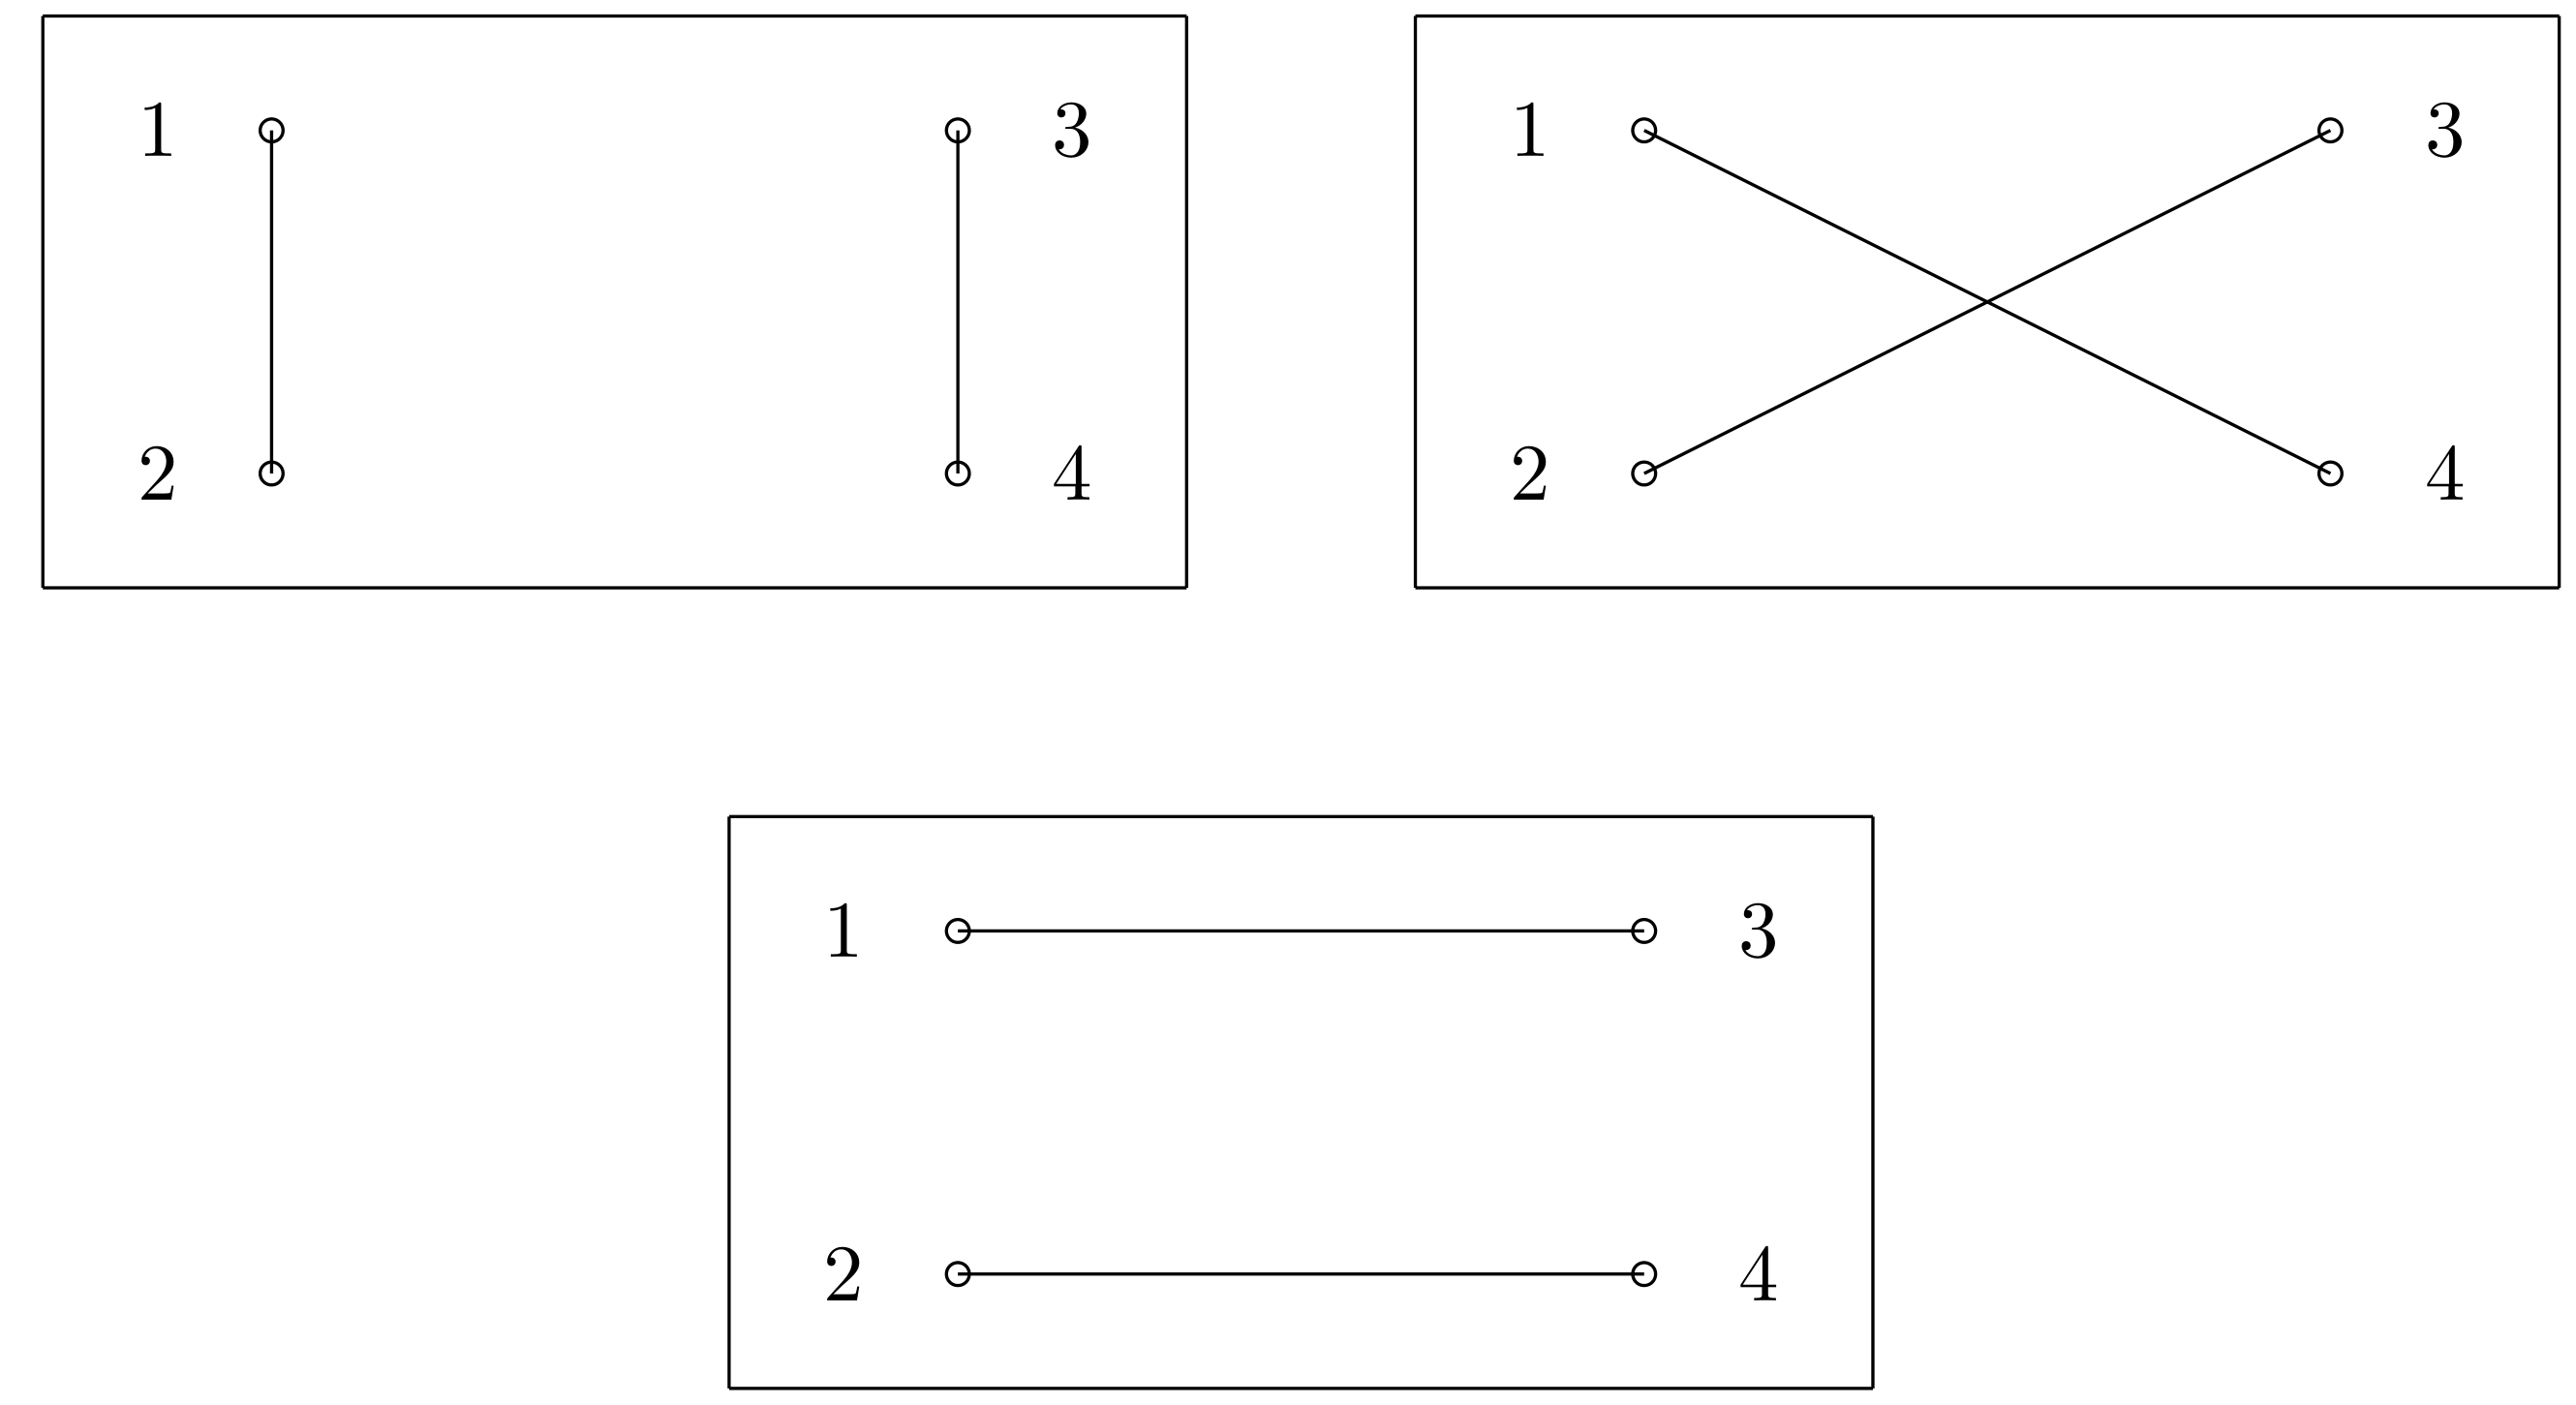
\includegraphics[width=11.26cm]{figures/fig-01.png}
  \caption{集合 $\{1, 2, 3, 4 \}$ 的配对\figorig{29}{1}}
  \label{fig:1}
\end{figure}


我们用 $\Pi(T)$ 表示集合 $T$ 上所有配对构成的集合，并把 $\Pi(\lbrace{1, \ldots ,2k\rbrace})$ 记作 $\Pi_k$。显然 $|\Pi_k|=\frac{(2k)!}{2^k\cdot k!}=(2k-1)!!$。对任意 $\sigma\in \Pi_k$，可把 $\sigma$ 看作 $\lbrace{1, \ldots ,2k\rbrace}$ 的一个置换，满足 $\sigma^2=1$ 且 $\sigma$ 没有不动点。也就是说，$\sigma$ 把任一元素 $i$ 映到含 $i$ 的那一对中的另一个元素 $\sigma(i)$。

\begin{theorem}\label{wick}（Wick 定理）设 $B^{-1}$ 表示 $B$ 在 $V^*$ 上的逆形式，$\ell_1, \ldots ,\ell_N\in V^*$。
则当 $N$ 为偶数时，有
$$
\int_{V}\ell_1(x) \ldots \ell_N(x)e^{-\frac{B(x,x)}{2}}dx=
\frac{(2\pi)^{\frac{d}{2}}}{\sqrt{\det B}}
\sum_{\sigma\in \Pi_{N/2}}\prod_{i\in \lbrace{1, \ldots ,N\rbrace}/\sigma}
B^{-1}(\ell_i,\ell_{\sigma(i)})
$$
当 $N$ 为奇数时，该积分为零。
\end{theorem}

\begin{proof} 若 $N$ 为奇数，结论显然，因为被积函数是奇函数。故考虑偶数情形 $N=2k$。
由于等式两边都是 $\ell_1, \ldots ,\ell_N$ 的对称多重线性型，
只需在 $\ell_1= \cdots =\ell_N=\ell$ 时证明结论。
此外，显然所讨论的公式在线性变量替换下不变，
因此可以选取坐标系使 $B(x,x)=x_1^2+ \cdots +x_d^2$、$\ell(x)=x_1$。
于是只需假设 $d=1$ 且 $\ell(x)=x$。
此时定理断言
$$
\int_{-\infty}^{\infty}x^{2k}e^{-\frac{x^2}{2}}dx=(2\pi)^{\frac{1}{2}}(2k-1)!!,
$$
这正是公式 \eqref{gammaint}。
\end{proof}

\begin{example} 我们有
$$
\int_{V}\ell_1(x)\ell_2(x)e^{-\frac{B(x,x)}{2}}dx=
\frac{(2\pi)^{\frac{d}{2}}}{\sqrt{\det B}}
B^{-1}(\ell_1,\ell_2),
$$
\scriptsize
$$
\int_{V}\ell_1(x)\ell_2(x)\ell_3(x)\ell_4(x)e^{-\frac{B(x,x)}{2}}dx=
$$
$$
\frac{(2\pi)^{\frac{d}{2}}}{\sqrt{\det B}}
(B^{-1}(\ell_1,\ell_2)B^{-1}(\ell_3,\ell_4)+
B^{-1}(\ell_1,\ell_3)B^{-1}(\ell_2,\ell_4)+
B^{-1}(\ell_1,\ell_4)B^{-1}(\ell_2,\ell_3)).
$$
\normalsize
\end{example}

Wick 定理表明，$a_i$ 的计算问题具有组合本性。事实上，在这一计算中起核心作用的是某些有限图，称为\emph{Feynman 图}。它们是本节余下部分的主要研究对象。

% [Tutor Note: 计数要点——$2k$ 个标记点的配对数满足 $|\Pi_k|=\frac{(2k)!}{2^k k!}=(2k-1)!!$：先对 $2k$ 个点排序（$2k!$ 种），再除以每对的顺序 $2^k$ 与各对之间的顺序 $k!$。这与高斯矩 $\int x^{2k}e^{-x^2/2}dx=(2k-1)!!\sqrt{2\pi}$ 的系数完全一致；定理证明中“令 $\ell_1=\cdots=\ell_N=\ell$ 再作正交变换把 $B$ 化为标准形”是化归到 $d=1$ 的关键，但这一步只对多重线性型成立，$g$ 为一般多项式时不能这样化归。自由理论的归一化因子 $(2\pi)^{d/2}/\sqrt{\det B}$ 恰是“无边图的真空振幅”，可用作核对后续 Feynman 规则中每个连通分量的整体系数。]

\subsection{Feynman 图与 Feynman 定理} \label{fdft}
我们回到系数 $a_i$ 的计算问题。
由于每个具体的 $a_i$ 只依赖于 $g$ 在 $c$ 处的有限阶导数，故不妨假设 $g$ 是多项式，或更具体地说，是线性函数之积：
$g=\ell_1 \ldots \ell_N$，$\ell_i\in V^*$。因此，只需能够计算积分
\begin{equation}\label{expaa}
\langle\ell_1 \ldots \ell_N\rangle:= \hbar^{-\frac{d}{2}}e^{\frac{S(c)}{\hbar}}\int_{D}
\ell_1(x) \ldots\ell_N(x)e^{-\frac{S(x)}{\hbar}}dx.
\end{equation}
的级数展开。

不失一般性，可设 $c=0$ 且 $S(c)=0$。
于是 $S$ 在 $c$ 处的（渐近）Taylor 展开为
$$
S(x)=\frac{B(x,x)}{2}-\sum_{i\ge 3}\frac{B_i(x,\ldots,x)}{i!},
$$
其中 $B_i:=d^if(0)$。因此，把 \eqref{expaa} 的左端视为 $\hbar$ 的幂级数，并作变量替换 $x\mapsto \hbar^{\frac{1}{2}}x$（与上一节相同），得到
$$
\langle\ell_1 \ldots \ell_N\rangle=
\hbar^{\frac{N}{2}}\int_V \ell_1(x) \ldots \ell_N(x)e^{-\frac{B(x,x)}{2}+
\sum_{i\ge 3}\hbar^{\frac{i}{2}-1}\frac{B_i(x, \ldots ,x)}{i!}}dx.
$$
注意，这只是在 $\hbar$ 的渐近展开意义下的等式，因为我们忽略了用全空间代替区域 $D$ 所产生的快速衰减误差。但它特别蕴涵：当 $\hbar\to 0$ 时 $\langle\ell_1 \ldots \ell_N\rangle=O(\hbar^{\lceil\frac{N}{2}\rceil})$（因为展开式中只含 $\hbar$ 的整数幂）。

下面的定理归功于 Feynman，它以 Feynman 图的形式给出该积分的值。
该定理容易证明，却是量子场论的核心，并将成为我们的主要定理之一。在陈述 Feynman 定理之前，先引入一些记号。

设 $G_{\ge 3}(N)$ 表示满足下述条件的图的同构类之集：有 $N$ 个 1 价“外”顶点，标记为 $1, \ldots ,N$；还有有限个无标记的“内”顶点，其价数任意且 $\ge 3$。注意这里及以下均允许图在两个顶点之间有多重边，也允许顶点到自身的自环（见图~\ref{fig:2}）。

\begin{figure}[htbp]
  \centering
  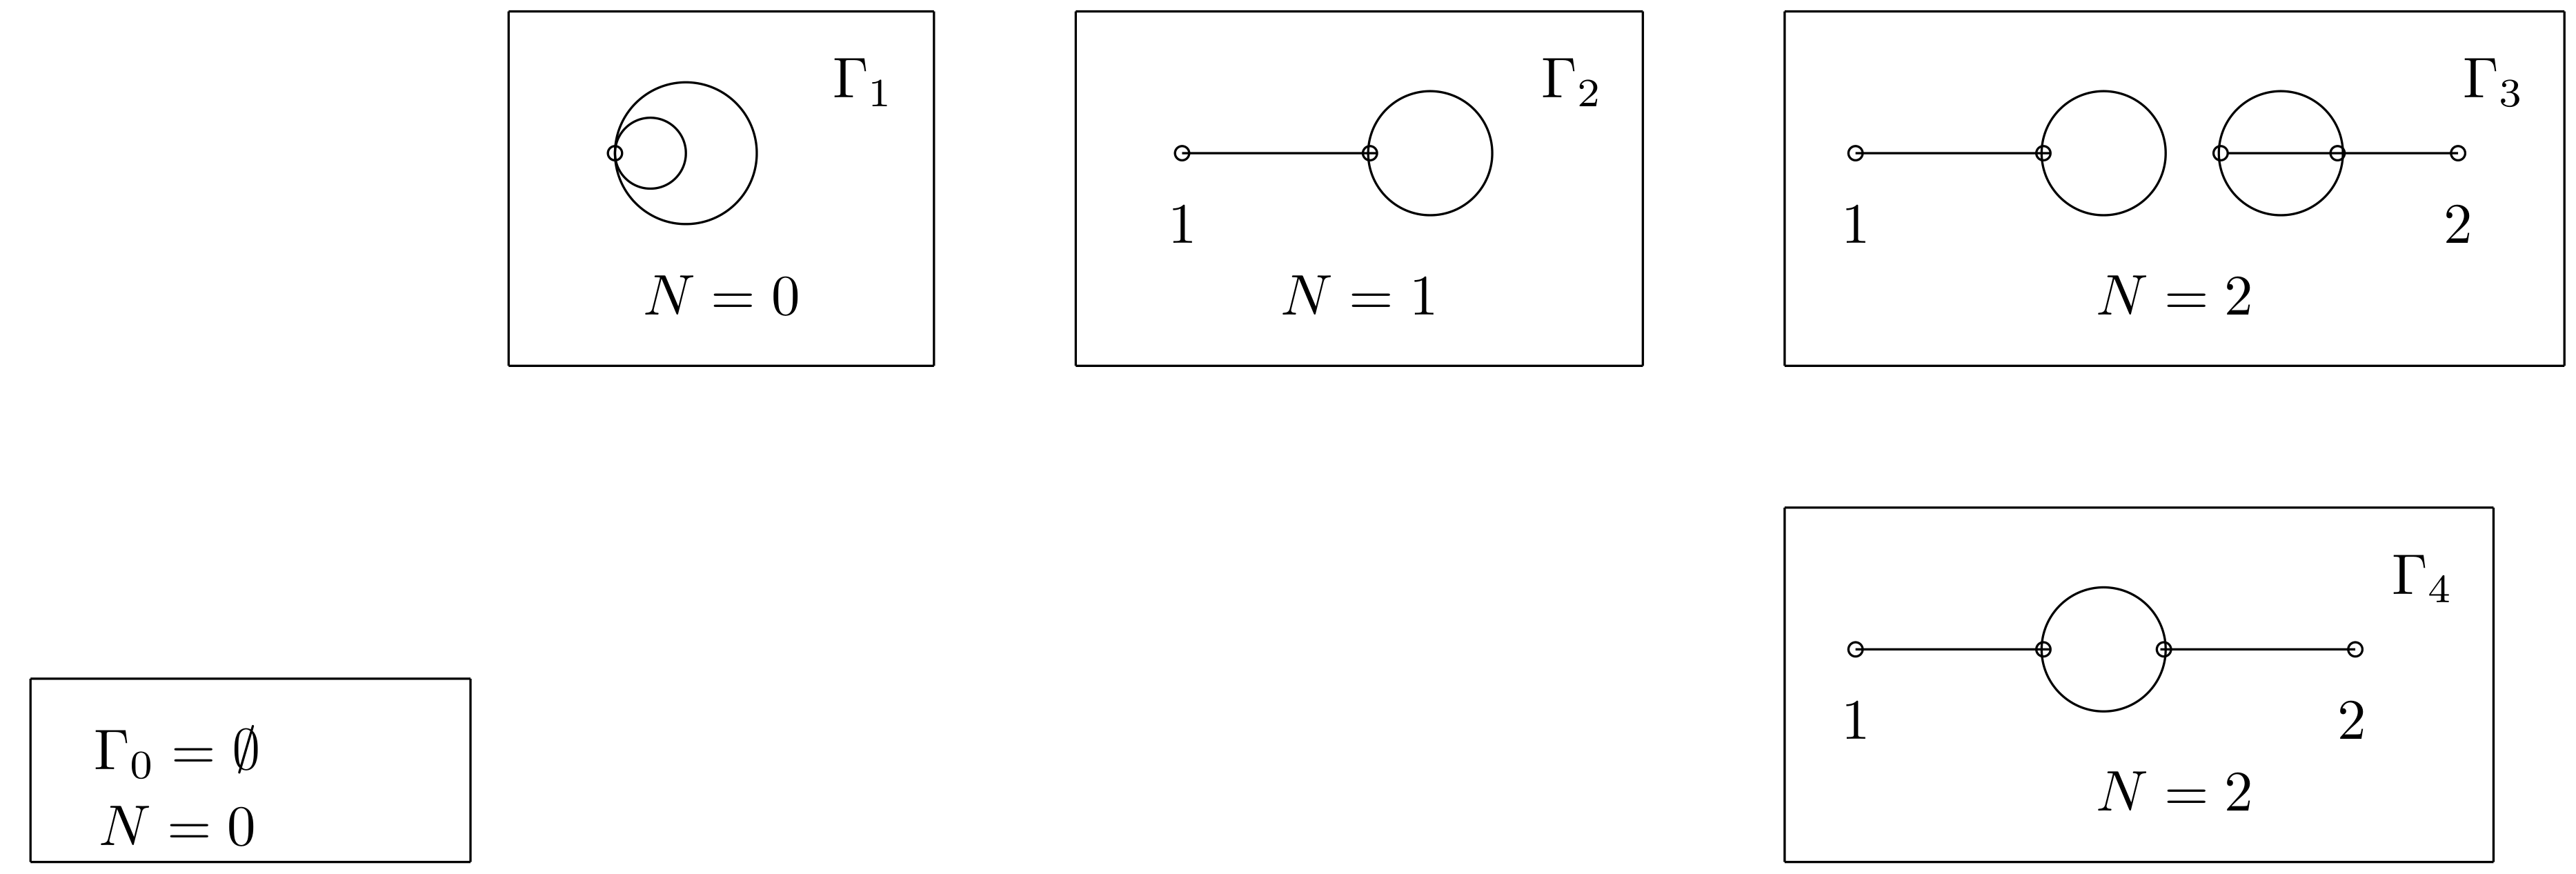
\includegraphics[width=15.6cm]{figures/fig-02.png}
  \caption{$G_{\ge 3} (N)$ 的元素示例。\figorig{31}{2}}
  \label{fig:2}
\end{figure}

对每个图 $\Gamma\in G_{\ge 3}(N)$，如下定义 $\Gamma$ 的\emph{Feynman 振幅}。

1. 把余向量 $\ell_j$ 放在第 $j$ 个外顶点上。

2. 在每个 $i$ 价内顶点上放张量 $B_i$。

3. 用双线性型 $B^{-1}$ 沿 $\Gamma$ 的边对这些张量作缩并。
由此得到一个数，称为 $\Gamma$ 的\emph{（Feynman）振幅}，记作 $F_\Gamma(\ell_1, \ldots ,\ell_N)$。

\begin{remark} 若 $\Gamma$ 不连通，则 $F_\Gamma$ 定义为各连通分量所得数之积。此外，空图的振幅定义为 $1$。
\end{remark}

\begin{example} 设
$$
B_3:=\sum_i b_i^{13}\otimes b_i^{23}\otimes b_i^{33},\ 
B_4:=\sum_j b_j^{14}\otimes b_j^{24}\otimes b_j^{34}\otimes b_j^{44},
$$
其中 $b_i^{jk}\in V^*$。则对图~\ref{fig:2} 中的图 $\Gamma_3$，其振幅等于
\scriptsize
$$
F_{\Gamma_3}(\ell_1,\ell_2)=
$$
$$
\sum_i B^{-1}(\ell_1,b_i^{13})B^{-1}(b_i^{23},b_i^{33})\cdot \sum_{i,j} B^{-1}(b_i^{13},b_j^{14})B^{-1}(b_i^{23},b_j^{24})B^{-1}(b_i^{33},b_j^{34})B^{-1}(b_j^{44},\ell_2).
$$
\normalsize
\end{example}

\begin{theorem}\label{Feyn}（Feynman）
有
\begin{equation}\label{Feynsum}
\langle\ell_1 \ldots \ell_N\rangle=
\frac{(2\pi)^{\frac{d}{2}}}{\sqrt{\det B}}
\sum_{\Gamma\in G_{\ge 3}(N)}\frac{\hbar^{b(\Gamma)}}{|{\rm Aut}(\Gamma)|}
F_\Gamma(\ell_1, \ldots ,\ell_N),
\end{equation}
其中 $b(\Gamma)$
是 $\Gamma$ 的边数减去内顶点数。
\end{theorem}
这里 ${\rm Aut}(\Gamma)$ 表示 $\Gamma$ 的自同构群；所谓 $\Gamma$ 的自同构，是指对顶点\textbf{与}边的一个置换（可以翻转自环），它固定每个外顶点并保持图的结构，见图~\ref{fig:3}。因此可能存在非平凡的自同构：有的在顶点集上作用平凡，有的甚至在边集上也作用平凡。例如，存在 $\Gamma_4$ 的一个自同构翻转上下两条弧，以及 $\Gamma_2$ 的一个自同构翻转自环。

\begin{figure}[htbp]
  \centering
  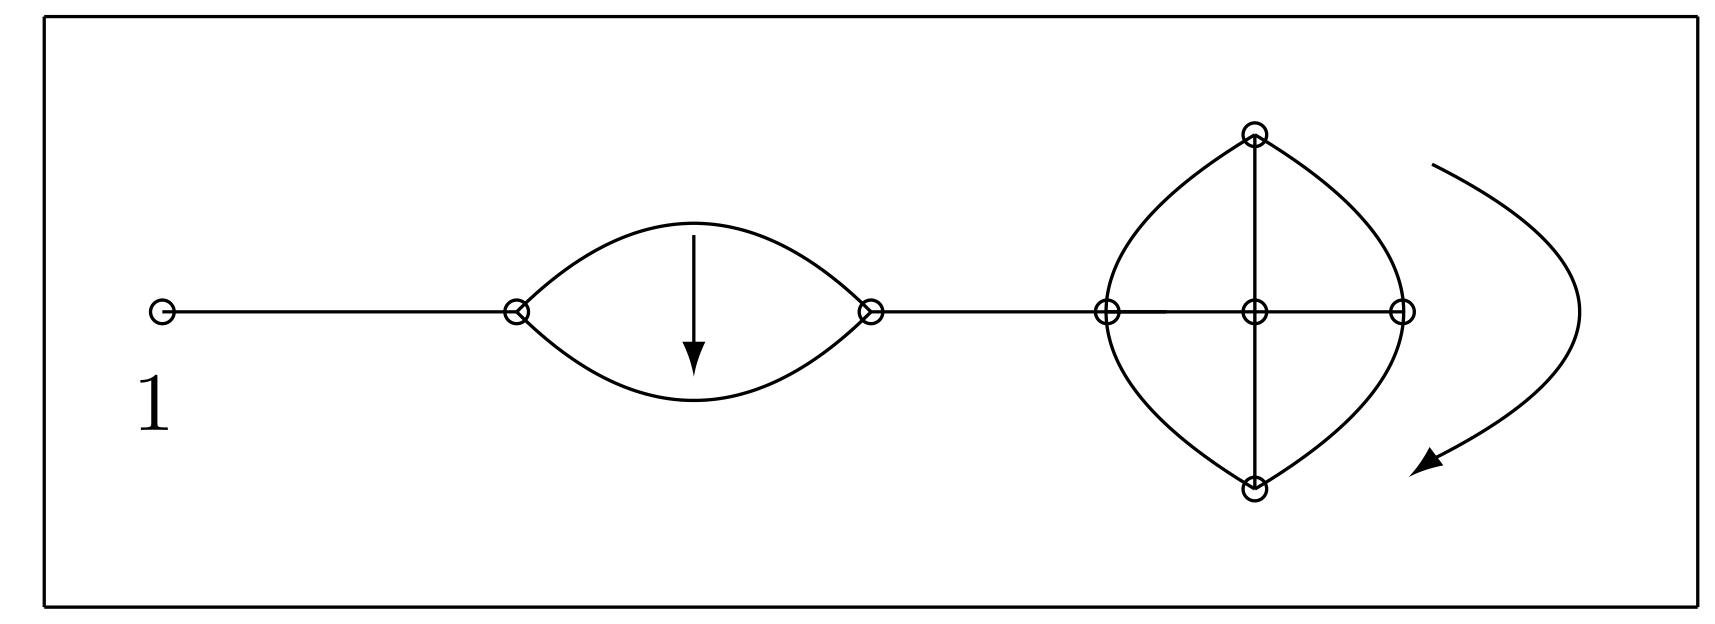
\includegraphics[width=7.26cm]{figures/fig-03.png}
  \caption{图的一个自同构\figorig{32}{3}}
  \label{fig:3}
\end{figure}


\begin{remark} 1. 注意这个和是无穷和，但按 $\hbar$ 的幂次形式收敛（形式幂级数意义下收敛）。

2. 定理 \ref{Feyn} 是 Wick 定理的推广：取 $S(x)=\frac{B(x,x)}{2}$ 即得后者。事实上，此时给出非零振幅的图没有内顶点，故归结为对应于配对 $\sigma$ 的图。
\end{remark}

现在对术语作一些说明。在量子场论中，函数 $\langle\ell_1 \ldots \ell_N\rangle$ 称为\emph{N 点关联函数}，图 $\Gamma$ 称为\emph{Feynman 图}。置于边上的型 $B^{-1}$ 称为\emph{传播子}。函数 $S$ 的展开中的三次及更高次项 $\frac{B_i}{i!}$ 称为\emph{相互作用项}，因为这类项（在作用量泛函中）描述粒子间的相互作用。$S$ 为二次型（即无相互作用）的情形称为\emph{自由理论}；也就是说，对自由理论，关联函数由 Wick 公式确定。

\begin{remark}\label{G3*} 有时考虑归一化关联函数是方便的：
$$
\langle\ell_1\ldots\ell_N\rangle_{\rm norm}:=\frac{\langle\ell_1\ldots\ell_N\rangle}{\langle\emptyset\rangle}
$$
其中 $\langle\emptyset\rangle$ 表示无插入时的积分。
Feynman 定理蕴涵它们由下述公式给出：
$$
\langle\ell_1 \ldots \ell_N\rangle_{\rm norm}=
\sum_{\Gamma\in G_{\ge 3}^*(N)}\frac{\hbar^{b(\Gamma)}}{|{\rm Aut}(\Gamma)|}
F_\Gamma(\ell_1, \ldots ,\ell_N),
$$
其中 $G^*_{\ge 3}(N)$ 是 $G_{\ge 3}(N)$ 中所有不含没有外顶点的连通分量的那些图构成的子集。
\end{remark}

% [Tutor Note: 对称因子——定理中的 $|{\rm Aut}(\Gamma)|$ 必须连同边一起计算：除顶点置换外，交换两条平行边、以及翻转自环（如原文中 $\Gamma_2$ 的自环、$\Gamma_4$ 的上下弧）都算非平凡自同构。检验办法：把图的所有半边（half-edge）视为可区分对象，$\prod_i i!^{n_i}n_i!$ 是“半边标记方式数”，除以 $|{\rm Aut}(\Gamma)|$ 才是同一图的相异标记数（轨道—稳定子定理）；对 $N$ 点函数，外顶点标记固定，故 $(2N-1)!!$ 只出现在无内顶点的 Wick 情形，一般图没有简单的双阶乘公式。]

% [Tutor Note: 原文疑误——第 2 小节中 $B_i:=d^if(0)$ 的 $f$ 应为 $S$，即 $B_i:=d^iS(0)$；由上下文 $S(x)=\frac{B(x,x)}{2}-\sum_{i\ge3}B_i(x,\ldots,x)/i!$ 亦可判定。另外术语一段 “propagator” 后原文多写了一个句点（“propagator}..”），译文按单句点处理。]

\subsection{Feynman 定理的加权版本}
在证明定理 \ref{Feyn} 之前，我们先对它略作修改与推广。即在量子场论中，常把相互作用理论视为自由理论的形变。
这意味着 $S(x)=\frac{B(x,x)}{2}+\widetilde S(x)$，其中 $\widetilde S(x)$ 是微扰
$$
\widetilde S(x):=-\sum_{i\ge 0}g_i\frac{B_i(x, \ldots ,x)}{i!}
$$
而 $g_r, r\ge 0$ 是（形式）参数。这些参数的一个好处是：它们使我们能按各价数顶点的数目，对和式 \eqref{Feynsum} 中 Feynman 图的振幅进行归并。
具体地说，把\emph{配分函数}
$$
Z=\hbar^{-\frac{d}{2}}\int_V e^{-\frac{S(x)}{\hbar}}dx
$$
视为 $g_i$ 的级数。
设 $\bold n=(n_0,n_1,n_2, \ldots )$ 是非负整数序列，其中几乎所有的项都为零。
设 $G(\bold n)$ 表示具有 $n_0$ 个 0 价顶点、$n_1$ 个 1 价顶点、$n_2$ 个 2 价顶点等的图的同构类之集
（因此，现在考虑的是无外顶点的图）。对 $\Gamma\in G(\bold n)$，以 $F_\Gamma$ 记如前定义的 $\Gamma$ 的振幅。于是
$$
F_\Gamma=\prod_i{g_i^{n_i}}\cdot \Bbb F_\Gamma, 
$$
其中 $\Bbb F_\Gamma$ 是不含因子 $g_j$ 时算得的 Feynman 振幅。

\begin{theorem}\label{Feyn1}
有
$$
Z=
\frac{(2\pi)^{\frac{d}{2}}}{\sqrt{\det B}}
\sum_{\bold n}
\sum_{\Gamma\in G(\bold n)}\frac{\hbar^{b(\Gamma)}}{|{\rm Aut}(\Gamma)|}
F_\Gamma=
$$
$$
\frac{(2\pi)^{\frac{d}{2}}}{\sqrt{\det B}}
\sum_{\bold n}\prod_i({g_i\hbar^{\frac{i}{2}-1})^{n_i}}
\sum_{\Gamma\in G(\bold n)}\frac{\Bbb F_\Gamma}{|{\rm Aut}(\Gamma)|},
$$
其中 $b(\Gamma)=\sum_i n_i(\frac{i}{2}-1)$
是 $\Gamma$ 的边数减去顶点数。
\end{theorem}

注意，可以把 $Z$ 视为代数
$$
\Bbb C[g_0\hbar^{-\frac{3}{2}},g_1\hbar^{-1},g_2\hbar^{-\frac{1}{2}}; g_j,j\ge 3][[\hbar^{\frac{1}{2}}]],
$$
的元素，亦即它可以特殊化为
$$
g_0\hbar^{-\frac{3}{2}},g_1\hbar^{-1},g_2\hbar^{-\frac{1}{2}},g_3,g_4,...,
$$
的数值，从而给出 $\Bbb C[[\hbar^{\frac{1}{2}}]]$ 中的一个元素。
此外，$Z$ 也可特殊化到 $\hbar=1$，得到 $\Bbb C[[g_j, j\ge 0]]$ 中的一个元素；而该定理实际上等价于这一特殊化。我们仍然选择保留 $\hbar$，是为了能够取经典极限 $\hbar\to 0$。

我们将在下一小节证明定理 \ref{Feyn1}。
这里先说明定理 \ref{Feyn} 实际上是定理 \ref{Feyn1} 的特例。
事实上，由于关联函数关于 $\ell_1, \ldots ,\ell_N$ 对称，只需考虑 $\ell_1= \cdots =\ell_N=\ell$ 的情形。
此时记关联函数 $\langle\ell^N\rangle$（即 $\ell^N$ 的期望值）。显然，为对所有 $N$ 计算 $\langle\ell^N\rangle$，只需计算生成函数
$$
\langle e^{\ell}\rangle=\hbar^{-\frac{d}{2}}\int_Ve^{\ell(x)-\frac{S(x)}{\hbar}}dx:=\sum_{N=0}^\infty \frac{\langle\ell^N\rangle}{N!},
$$
它在相差一个缩放因子以及把 $\ell$ 乘以 $i$ 的意义下，就是 Feynman 密度 $e^{-\frac{S(x)}{\hbar}}dx$ 的 Fourier 变换。但这个期望值恰好就是定理 \ref{Feyn1} 在 $g_i=1$（$i\ge 3$）、$g_0=g_2=0$、$g_1=\hbar $、$B_1=\ell$、$B_0=0$、$B_2=0$ 时给出的期望值。因此，定理 \ref{Feyn1} 蕴涵定理 \ref{Feyn}（分母中的因子 $N!$ 可由下述事实解释：定理 \ref{Feyn1} 中考虑的是无标记的 1 价顶点，而不是有标记的）。

\subsection{Feynman 定理的证明}
现在证明定理 \ref{Feyn1}。
作变量替换 $y=\hbar^{-\frac{1}{2}}x$。
把指数函数展开为 Taylor 级数，得
$$
Z=\sum_{\bold n}Z_\bold n, 
$$
其中
$$
Z_\bold n=\int_V e^{-\frac{B(y,y)}{2}}
\prod_i \frac{g_i^{n_i}}{i!^{n_i}n_i!}
(\hbar^{\frac{i}{2}-1}B_i(y, \ldots ,y))^{n_i}dy.
$$
把 $B_i$ 写成线性函数之积的和，并利用 Wick 定理可知，对每个 $\bold n$，该积分的值可以如下组合地表达。

1. 对每个因子 $B_i$ 配一朵“花”——一个带 $i$ 条出边的顶点（见图~\ref{fig:4}）。

\begin{figure}[htbp]
  \centering
  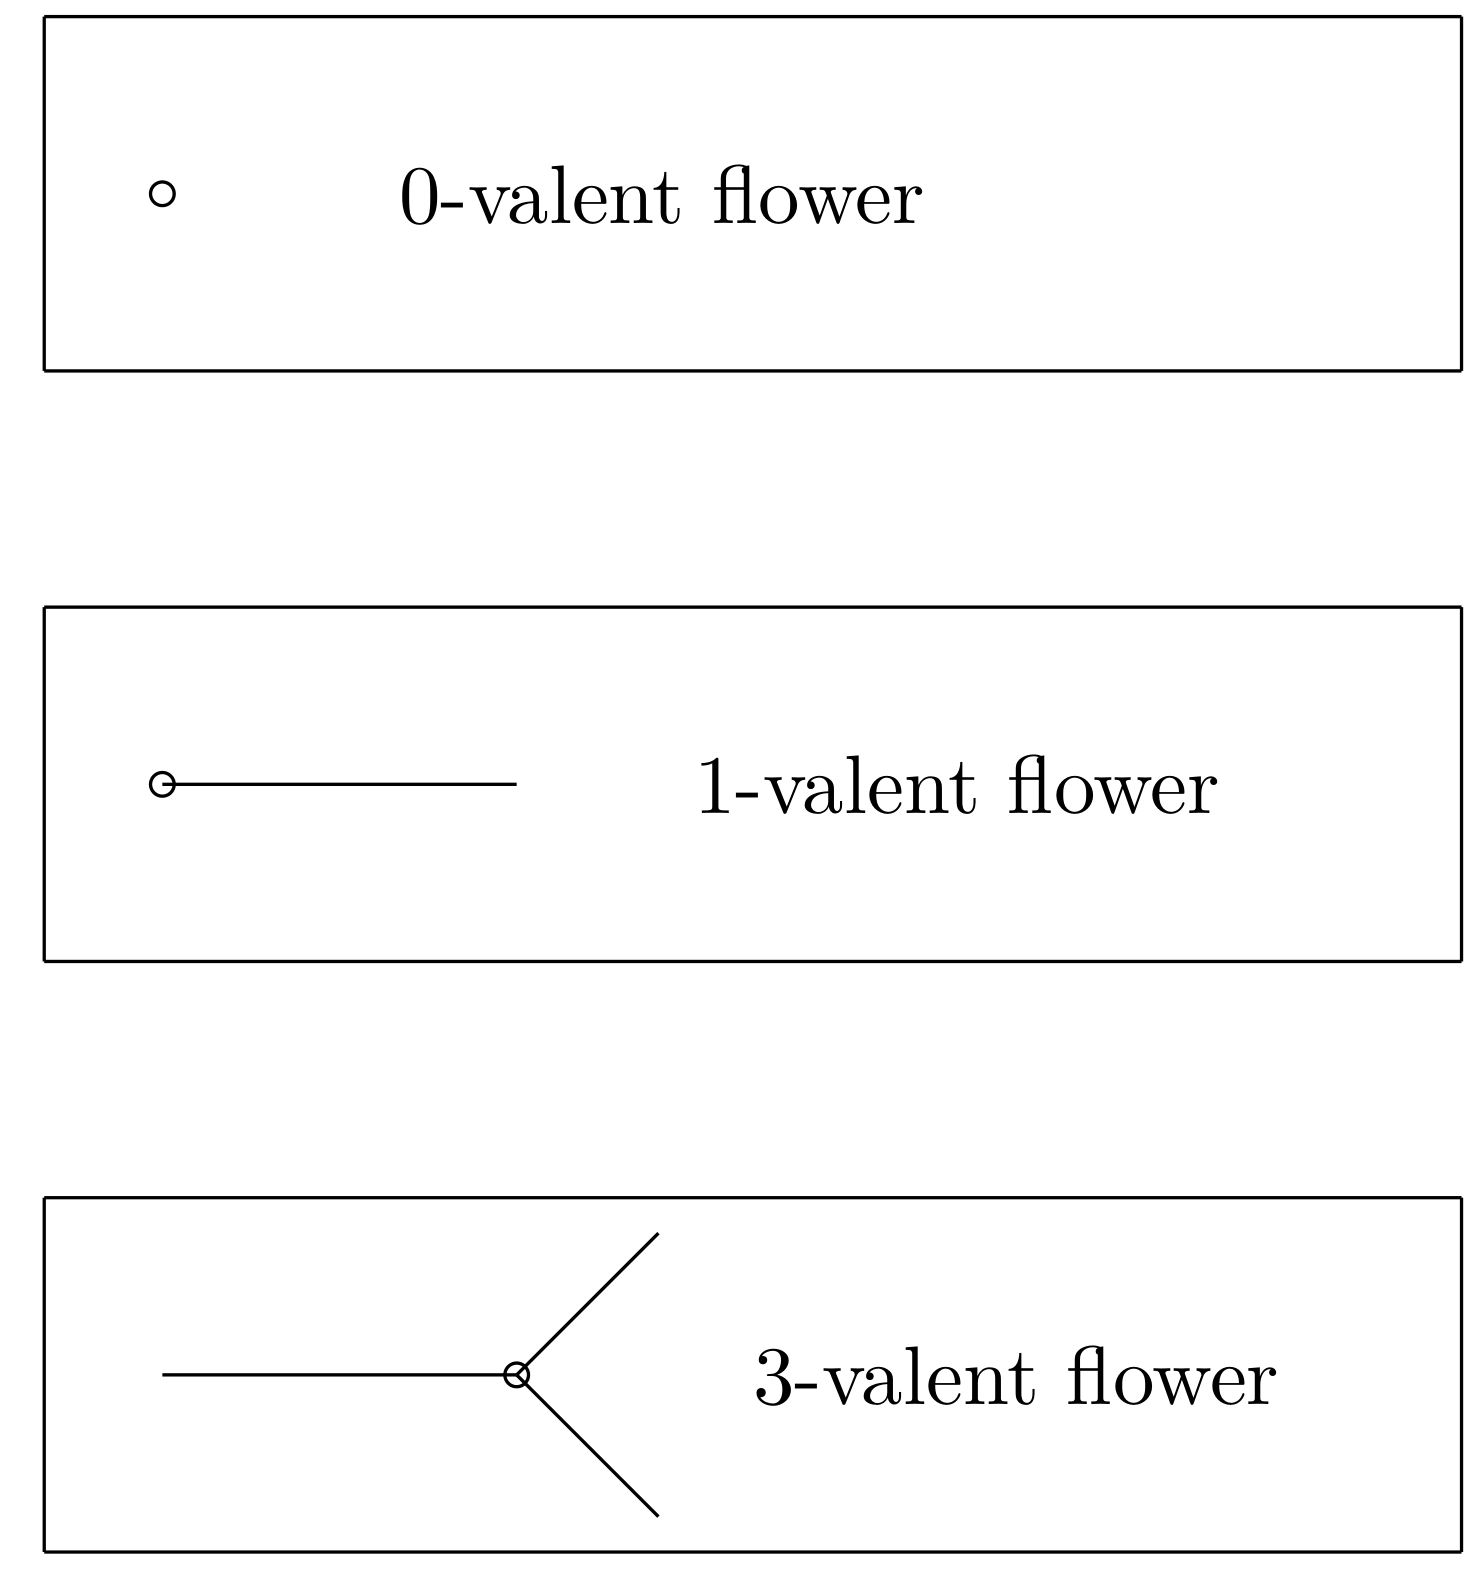
\includegraphics[width=6.26cm]{figures/fig-04.png}
  \caption{（原文无图题）\figorig{35}{4}}
  \label{fig:4}
\end{figure}


2. 考虑这些出边的端点构成的集合 $T_{\bold n}$（见图~\ref{fig:5}），并对该集合的任一配对 $\sigma$，考虑用型 $B^{-1}$ 对张量 $B_i$ 所作的相应缩并。由此得到标量 $\Bbb F(\sigma)$。

\begin{figure}[htbp]
  \centering
  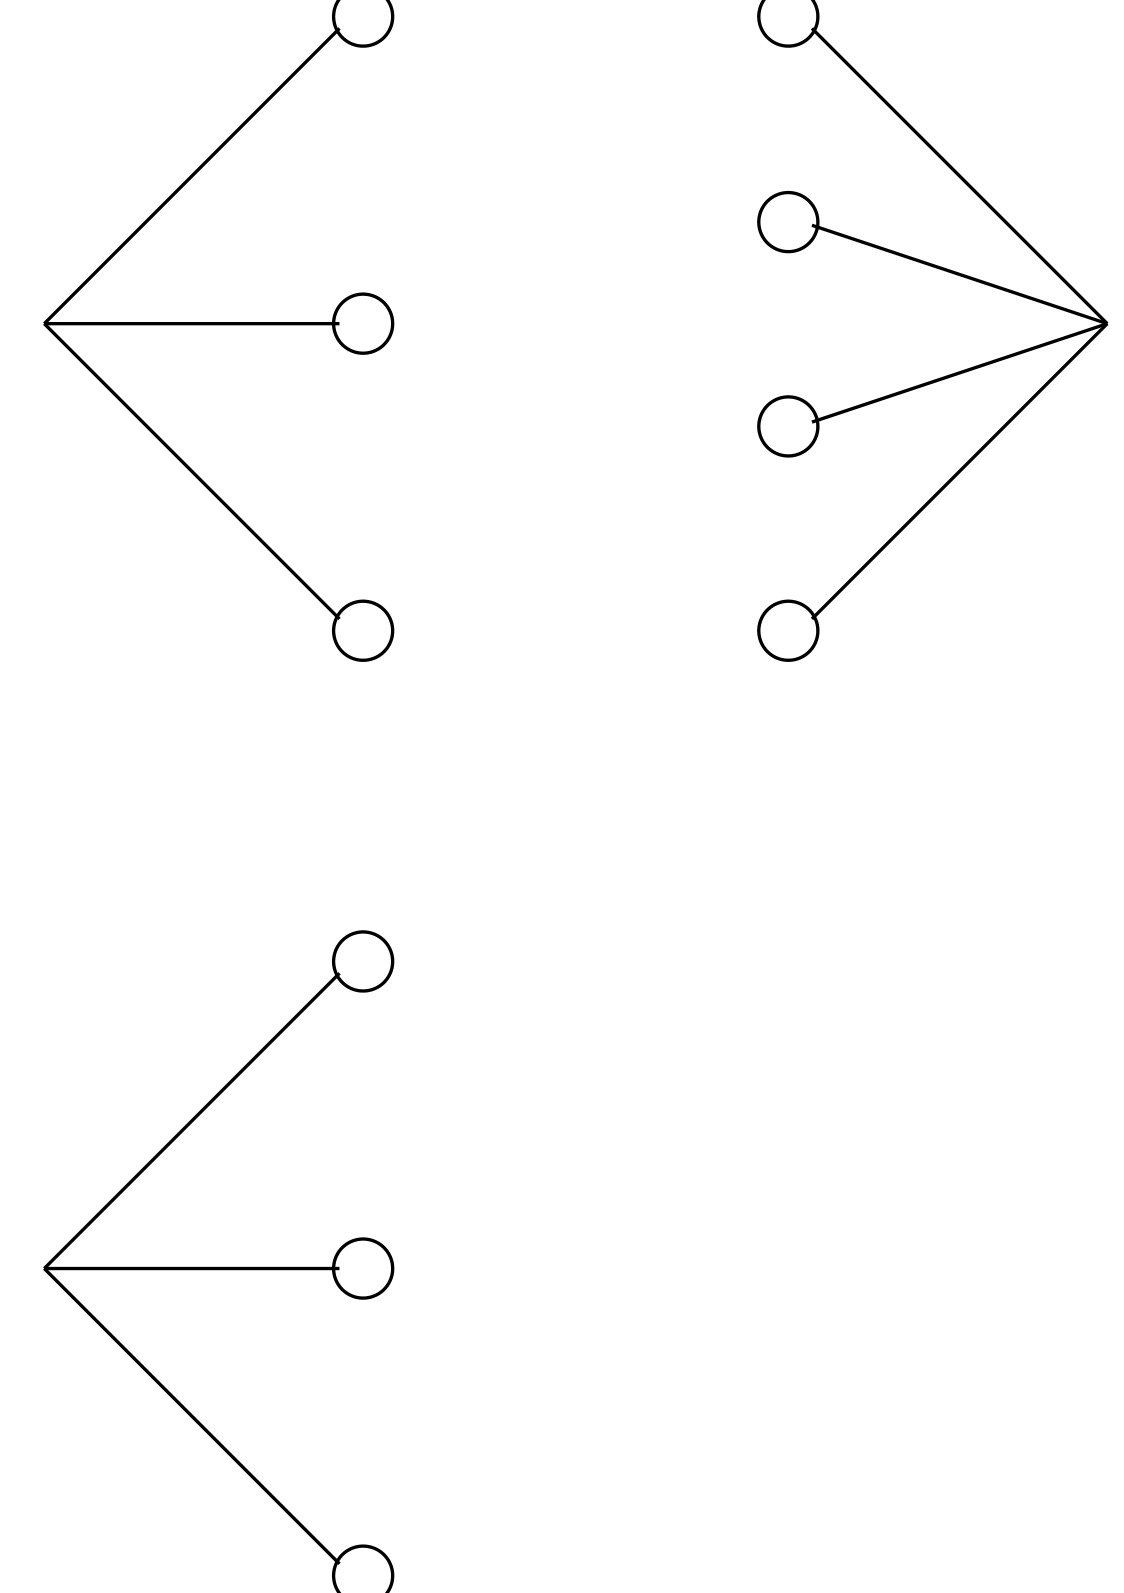
\includegraphics[width=4.76cm]{figures/fig-05.png}
  \caption{$\bold n = (0, 0, 0, 2, 1, 0, 0,       \ldots)$ 时的集合 $T_\bold n$（白色圆圈构成的集合）\figorig{35}{5}}
  \label{fig:5}
\end{figure}


3. 积分 $Z_{\bold n}$ 由下式给出：
\begin{equation}\label{sumpair}
Z_{\bold n}=\frac{(2\pi)^{\frac{d}{2}}}{\sqrt{\det B}}\prod_i
\frac{g_i^{n_i}}{i!^{n_i}n_i!}\hbar^{n_i(\frac{i}{2}-1)} \sum_{\sigma\in \Pi(T_{\bold n}) }\Bbb F(\sigma).
\end{equation}

现在回忆，集合上的配对可以这样可视化：把集合的元素画成点，并用边把它们连接起来。若对集合 $T_{\bold n}$ 这样做，则所有出边的端点都将以某种方式彼此连接，亦即得到一个（无向）图 $\Gamma=\Gamma_\sigma$（见图~\ref{fig:6}）。此外，容易看出标量 $\Bbb  F(\sigma)$ 正是振幅 $\Bbb F_\Gamma$。

\begin{figure}[htbp]
  \centering
  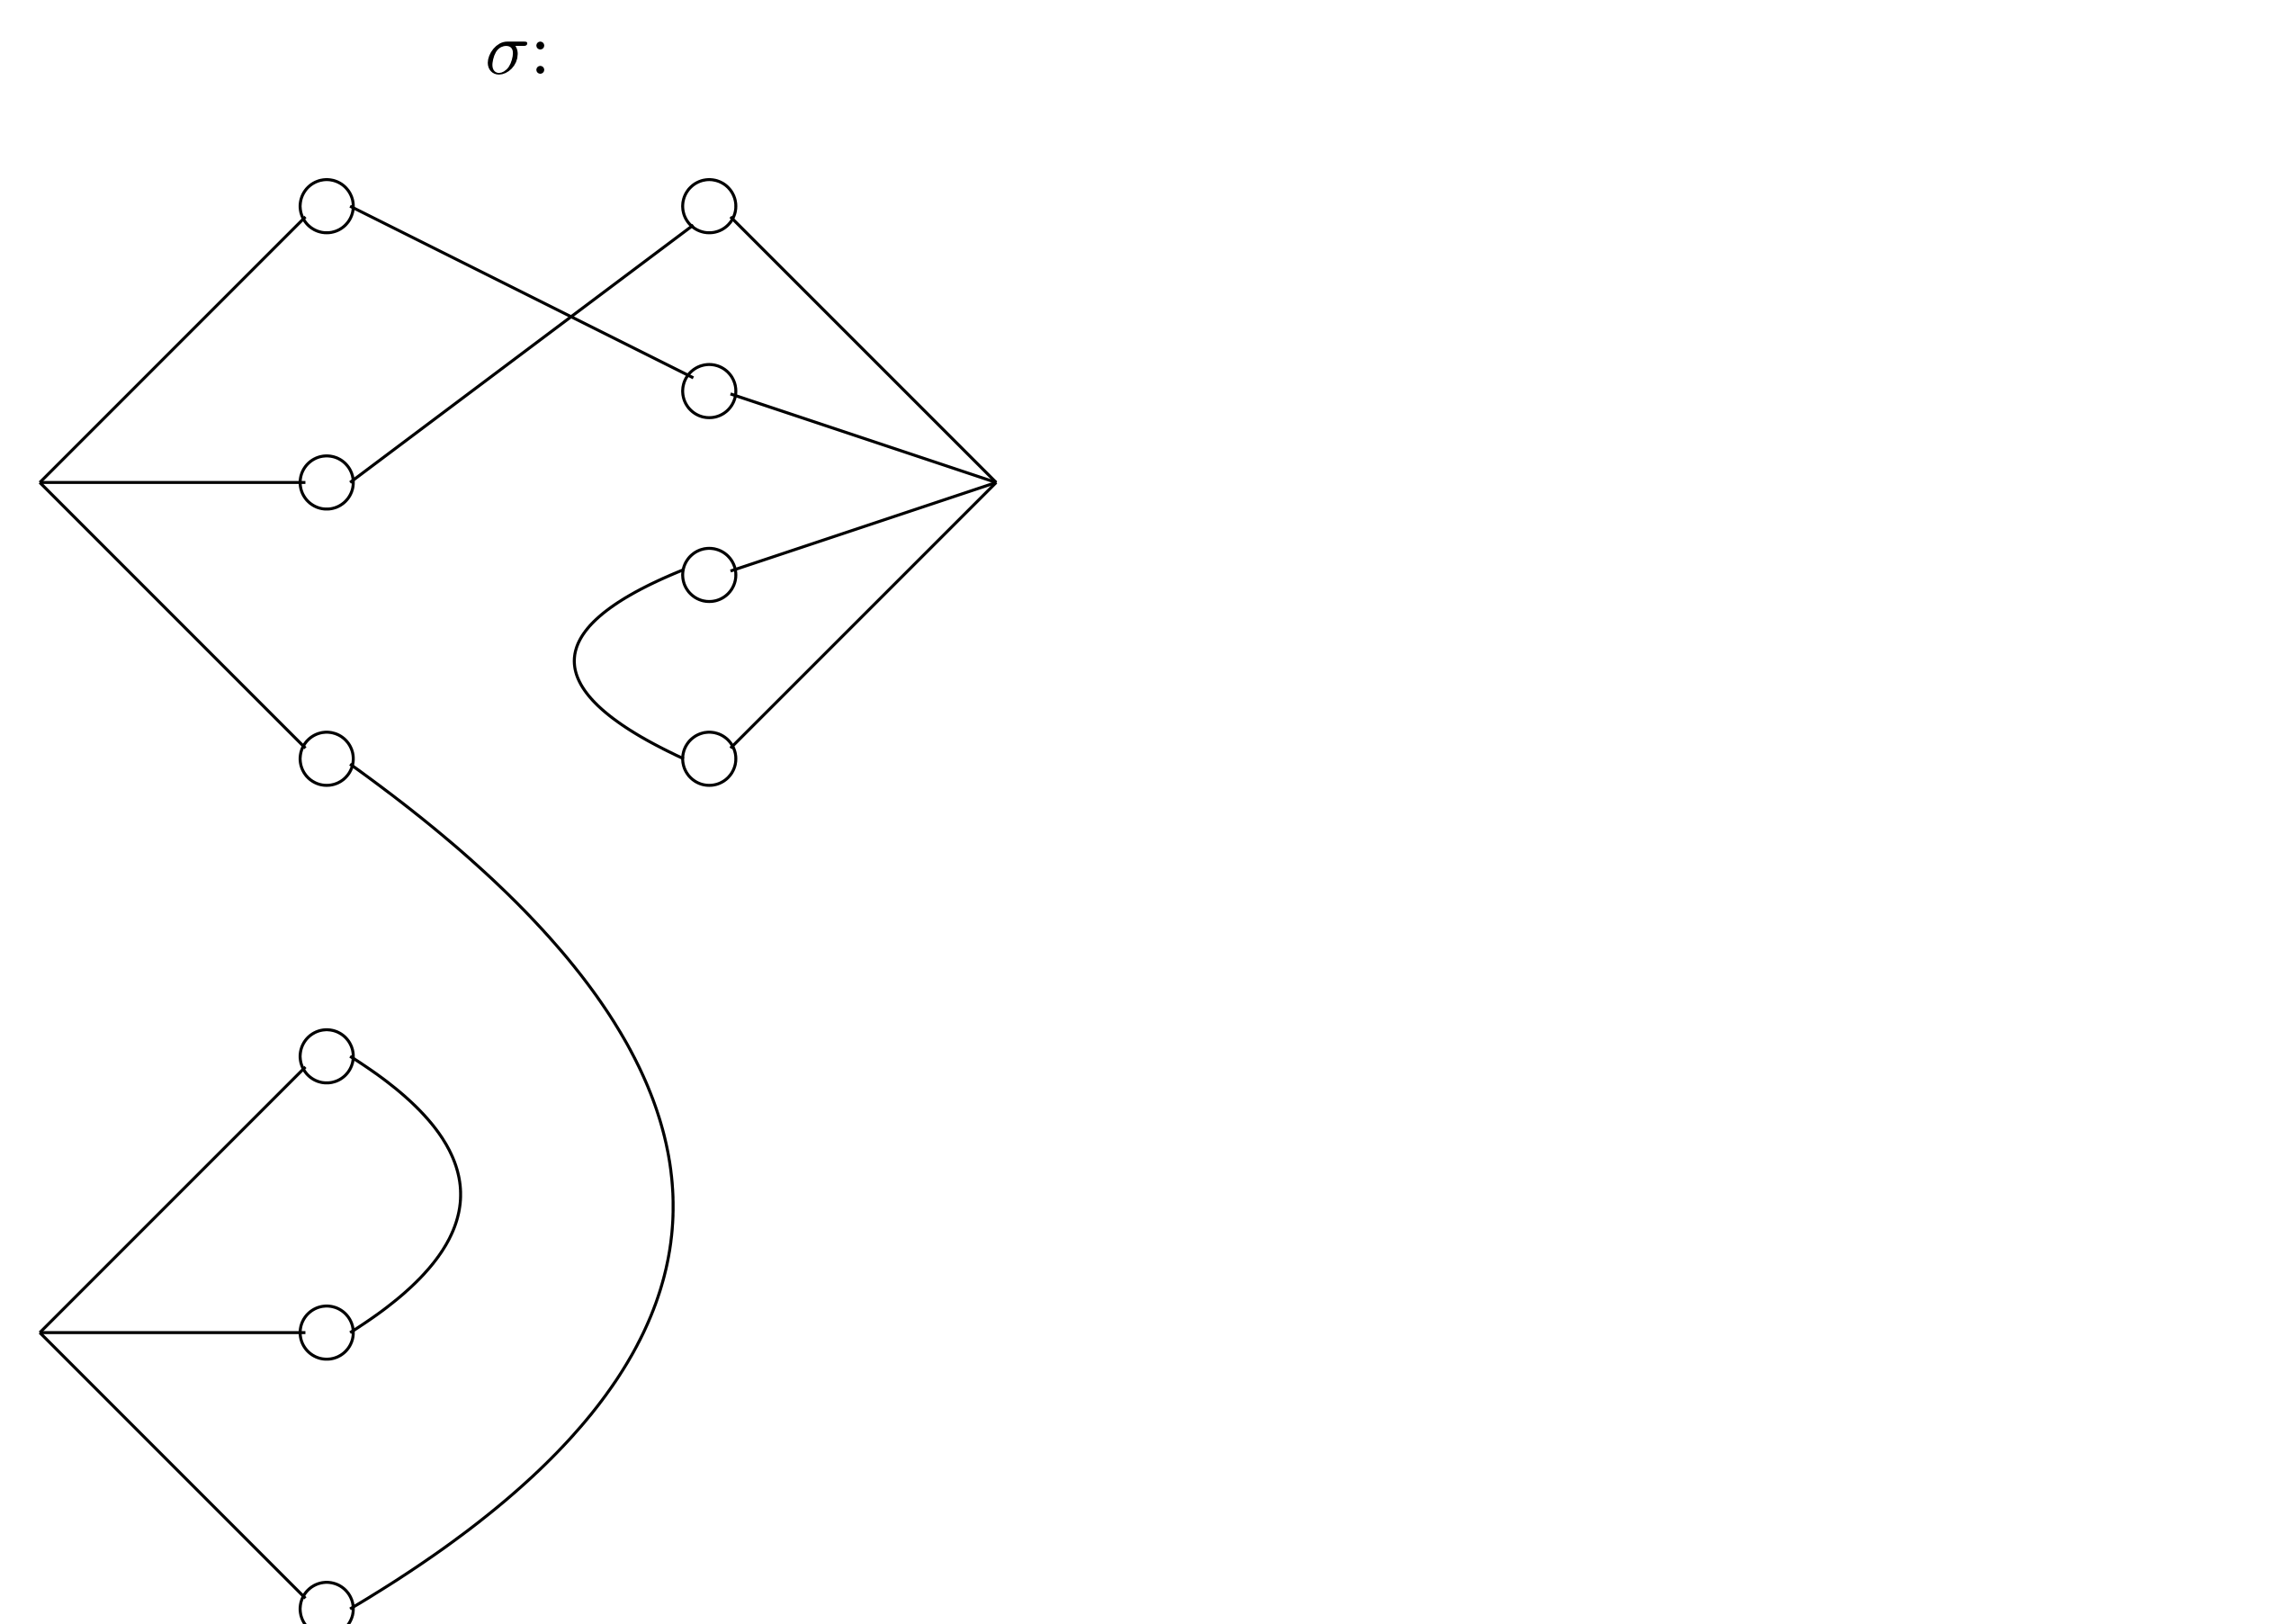
\includegraphics[width=10.76cm]{figures/fig-06.png}
  \caption{$T_{\bold n}$ 的一个配对 $\sigma$ 及相应的图 $\Gamma$。\figorig{36}{6}}
  \label{fig:6}
\end{figure}


显然，任一满足对每个 $i$ 有 $n_i$ 个 $i$ 价顶点的图 $\Gamma$ 都可由这种方式得到。然而同一个图可以以许多不同方式得到；因此，若想把对 $\sigma$ 求和中的相同项归并起来，并把它变成对 $\Gamma$ 的求和，就必须求出给出给定 $\Gamma$ 的 $\sigma$ 的数目。

为此，考虑 $T_{\bold n}$ 的保持“花”的置换群 $\Bbb G_{\bold n}$（即：从同一朵花出发的任意两条边的端点，经置换后仍落在同一朵花中）。该群包含：

1) 具有给定价数的各“花”之间的置换；

2) 每朵 $i$ 价“花”内部 $i$ 条边的置换。

更确切地说，群 $\Bbb G_{\bold n}$ 是对称群的半直积
$$
\Bbb G_{\bold n}=\prod_i (S_{n_i}\ltimes S_i^{n_i}).
$$
注意 $|\Bbb G_{\bold n}|=\prod_i i!^{n_i}n_i!$，它正是公式 (\ref{sumpair}) 分母中各数之积。

群 $\Bbb G_{\bold n}$ 作用在 $T_{\bold n}$ 的全部配对 $\sigma$ 构成的集合 $\Pi(T_{\bold n})$ 上。此外，它在给出给定图 $\Gamma$ 的 $T_{\bold n}$ 的配对构成的集合 $\Pi_\Gamma(T_{\bold n})$ 上传递地作用。进而容易看出，给定配对的稳定子就是 ${\rm Aut}(\Gamma)$。因此，给出 $\Gamma$ 的配对数等于
$$
N_\Gamma=\frac{\prod_i i!^{n_i}n_i!}{|{\rm Aut}(\Gamma)|}.
$$
于是
$$
\sum_{\sigma\in \Pi(T_{\bold n})} \Bbb F(\sigma)=\sum_\Gamma \frac{\prod_i i!^{n_i}n_i!}{|{\rm Aut}(\Gamma)|}
\Bbb F_\Gamma.
$$
最后注意，方程 (\ref{sumpair}) 中 $\hbar$ 的指数为 $\sum_in_i(\frac{i}{2}-1)$，它等于 $\Gamma$ 的边数减去顶点数，亦即 $b(\Gamma)$。
把它代入 (\ref{sumpair})，即得结论。

\begin{example}\label{treeexa} 取 $d=1$、$V=\Bbb R$、$g_i=g$、对所有 $i\ge 0$ 有 $B_i=z^i$（其中 $z$ 是形式变量）、$\hbar=1$。
于是得到渐近展开
$$
\frac{1}{\sqrt{2\pi}}\int_{-\infty}^\infty e^{-\frac{x^2}{2}+ge^{zx}}=
\sum_{n\ge 0}g^n\sum_{\Gamma\in G(n,k)}\frac{z^{2k}}{|{\rm Aut}(\Gamma)|},
$$
其中 $G(n,k)$ 是 $n$ 个顶点、$k$ 条边的图的同构类之集。\footnote{该积分在 $g<0$、$z\in \Bbb R$ 时收敛，但这在这里并不重要，因为我们只是形式地考虑该积分。}
展开左端，得
$$
\sum_k\sum_{\Gamma\in G(n,k)}\frac{z^{2k}}{|{\rm Aut}(\Gamma)|}=\frac{e^{\frac{z^2n^2}{2}}}{n!},
$$
从而
$$
\sum_{\Gamma\in G(n,k)}\frac{1}{|{\rm Aut}(\Gamma)|}=\frac{n^{2k}}{2^kk!n!}.
$$
\end{example}

\begin{exercise} 用直接组合计数验证之。
\end{exercise}

% [Tutor Note: 连通性取对数（指数公式）——定理 \ref{Feyn2} 的证明本质上是说：设 $Z/Z_0=\sum_\Gamma w_\Gamma$，其中 $w_\Gamma=\hbar^{b(\Gamma)}\Bbb F_\Gamma/|{\rm Aut}(\Gamma)|$ 按连通分量乘性分解。任一图可唯一写成连通图的 $k_j$ 重不交并 $\Gamma_1^{k_1}\ldots\Gamma_l^{k_l}$，故 $\sum_\Gamma w_\Gamma=\prod_j\sum_{k_j\ge0}w_{\Gamma_j}^{k_j}/k_j!=\exp\bigl(\sum_{\Gamma\ \text{连通}}w_\Gamma\bigr)$；其中 $1/k_j!$ 来自 $k_j$ 个同构副本之间的置换对称性，恰与自同构群阶中的 $k_j!$ 因子相消。这正是配分函数的连通图（团簇）展开，物理上即“自由能/连通关联取对数”。注意归一化 $Z/Z_0$ 已把空图振幅 $1$ 除掉，故 $\log$ 展开中没有整体常数项。]

\subsection{连通图求和}
下面将说明，配分函数 $Z$ 的对数同样由对图的求和给出，但只计入连通图。这大大简化了微扰论最初几阶中对 $Z$ 的分析，因为在给定顶点数与边数时，连通图的数目远小于全部图的数目。
\begin{theorem}\label{Feyn2} 设 $Z_0=\frac{(2\pi)^{\frac{d}{2}}}{\sqrt{\det B}}$。则有
$$
\log\frac{Z}{Z_0}=\sum_{\bold n}
\prod_i(g_i\hbar^{\frac{i}{2}-1})^{n_i}
\sum_{\Gamma\in G_c(\bold n)}\frac{\Bbb F_\Gamma}{|{\rm Aut}(\Gamma)|}
$$
其中 $G_c(\bold n)$ 是 $G(\bold n)$ 中连通图之集。\footnote{我们把连通图定义为恰有一个连通分量的图。因此，空图（连通分量数为零）不视为连通图。}
\end{theorem}

\begin{proof}
  对任意图 $\Gamma_1$、$\Gamma_2$，用 $\Gamma_1\Gamma_2$ 表示 $\Gamma_1$ 与 $\Gamma_2$ 的不交并；
  对任意图 $\Gamma$，用 $\Gamma^n$ 表示 $n$ 个 $\Gamma$ 的不交并。于是每个图都可唯一地
  写成 $\Gamma_1^{k_1} \ldots \Gamma_l^{k_l}$，其中 $\Gamma_j$
  是互不同构的连通图。此外，显然有
  $\Bbb F_{\Gamma_1\Gamma_2}=\Bbb F_{\Gamma_1}\Bbb F_{\Gamma_2}$、
  $b(\Gamma_1\Gamma_2)=b(\Gamma_1)+b(\Gamma_2)$，且
  $$
  |{\rm
    Aut}(\Gamma_1^{k_1} \ldots \Gamma_l^{k_l})|= \prod_j|{\rm
    Aut}(\Gamma_j)|^{k_j}k_j!.
    $$
    因此，把定理 \ref{Feyn2} 的等式取指数，并利用上述事实与函数 $e^x$ 的 Taylor 级数，
  即得定理 \ref{Feyn1}。既然定理 \ref{Feyn1} 已经证明，定理 \ref{Feyn2} 也就得证。
\end{proof}

\subsection{圈展开}
注意，由于定理 \ref{Feyn2} 中的求和是对连通 Feynman 图进行的，数 $b(\Gamma)$ 等于 $\Gamma$ 中的圈数减 1。特别地，$\hbar$ 的最低次项是 $\hbar^{-1}$ 项，它是对所有树的求和；次一项是 $\hbar^0$ 项，它是对所有含一个圈（回路）的图的求和；再下一项是 $\hbar$ 项，它是对双圈图的求和，依此类推。因此，物理学家把定理 \ref{Feyn2} 的展开称为\emph{圈展开}。

我们来研究这个展开中（关于 $\hbar$）最奇异的两项，即由树与单圈图求和给出的项。

设 $x_0$ 是函数 $S$ 的临界点。由于 $g_i$ 被假定为形式参数，它存在且唯一。
设 $G^{(j)}(\bold n)$ 表示 $G_c(\bold n)$ 中具有 $j$ 个圈的图的类之集。
令
$$
\left(\log\frac{Z}{Z_0}\right)_j:=
\sum_{\bold n}\prod_ig_i^{n_i}
\sum_{\Gamma\in G^{(j)}(\bold n)}\frac{\Bbb F_\Gamma}{|{\rm Aut}(\Gamma)|},
$$
于是
$$
\log\frac{Z}{Z_0}=\sum_{j=0}^\infty \left(\log\frac{Z}{Z_0}\right)_j \hbar^{j-1}.
$$

\begin{theorem}\label{trees1l}
\begin{equation}\label{treeeq}
\left(\log\frac{Z}{Z_0}\right)_0=-S(x_0),
\end{equation}
以及
\begin{equation}\label{1loopeq}
\left(\log\frac{Z}{Z_0}\right)_1=\frac{1}{2}\log \frac{\det B}{\det S''(x_0)}.
\end{equation}
\end{theorem}

\begin{proof}
首先注意，该命题纯属组合。
特别地，这意味着只需验证：当 $S$ 是实系数多项式、形如 $\frac{B(x,x)}{2}-\sum_{i=0}^Ng_i\frac{B_i(x, \ldots,x)}{i!}$ 且 $\hbar>0$ 时，命题给出的正是方程 (\ref{treeeq})、(\ref{1loopeq}) 右端的正确渐近展开。为此，令 $Z:=\hbar^{-\frac{d}{2}}\int_{\bold B}e^{-\frac{S(x)}{\hbar}}dx$，
其中 $\bold B$ 是以 $0$ 为心的球。
对充分小的 $g_i$，函数 $S$ 在 $\bold B$ 中有唯一的全局极小点 $x_0$，且该极小点非退化。
于是由最速下降公式，有
$$
\frac{Z}{Z_0}=e^{-\frac{S(x_0)}{\hbar}}I(\hbar), 
$$
其中 $I(\hbar)\sim\sqrt{\frac{\det B}{\det
    S''(x_0)}}(1+a_1\hbar+a_2\hbar^2+ \cdots )$（渐近地）。因此，
$$
\log\frac{Z}{Z_0}=-S(x_0)\hbar^{-1}+\frac{1}{2}\log
\frac{\det B}{\det S''(x_0)}+O(\hbar).
$$
这就蕴涵了结论。
\end{proof}

% [Tutor Note: 圈展开的幂次核对——对连通图，$V-E=1-L$（$L$ 为独立圈数），故 $b(\Gamma)=E-V=L-1$。逐顶点清点亦得同一结果：每个 $i$ 价顶点贡献 $\hbar^{i/2-1}$（来自 $x\mapsto\hbar^{1/2}y$ 的 $\hbar^{i/2}$ 乘以作用量中的 $\hbar^{-1}$），每条边（传播子 $B^{-1}$）贡献 $\hbar^0$，故总和为 $\sum_i n_i(\frac{i}{2}-1)=E-V$。树图 $L=0$ 给出 $\hbar^{-1}$ 的经典项 $-S(x_0)$，单圈给出 $\hbar^0$ 的 $\frac12\log\frac{\det B}{\det S''(x_0)}$，恰与第 2 章最速下降公式的指数前因子 $I(\hbar)\sim\sqrt{\det B/\det S''(x_0)}\,(1+O(\hbar))$ 逐项吻合，可作为检验译文与公式的独立手段。]

物理学家把表达式 $(\log\frac{Z}{Z_0})_0$ 称为对量子力学量 $\hbar\log\frac{Z}{Z_0}$ 的\emph{经典（或树）近似}，而把和 $(\log\frac{Z}{Z_0})_0+\hbar(\log\frac{Z}{Z_0})_1$ 称为\emph{单圈近似}。更高阶的圈近似可类似定义。注意，经典近似是通过求出经典作用量 $S(x)$ 的临界点与临界值而得到的；在经典力学与场论的情形，这对应于求解经典运动方程。

\bigskip
\noindent\rule{\textwidth}{0.6pt}
% [Tutor Note: 本章小结——Wick 定理是自由理论的全部内容：所有关联函数由 $(2k-1)!!$ 种两两缩并给出，$d=1$ 化归把一般正定二次型的情形归结为一维高斯矩。相互作用由 $\hbar^{i/2-1}$ 的顶点引入，Feynman 定理把关联函数写成对图的求和并配有对称因子 $1/|{\rm Aut}(\Gamma)|$；取对数后只剩连通图，$\hbar$ 的幂次直接数圈数。另注原文疑误：例 \ref{treeexa} 第一个渐近展开式右端为 $\sum_{n\ge0}g^n\sum_{\Gamma\in G(n,k)}z^{2k}/|{\rm Aut}(\Gamma)|$，其中 $k$ 未被求和（应由 $\sum_k$ 或 $G(n)$ 说明）；第二个式子按 $k$ 分组，可反推原意应为双层求和，译文照录原文。]


%=====================================================================
% 3  Feynman 演算（后半：3.7--3.14  非线性方程、树的计数与有效作用量）
% 原文：Section 3.7--3.14. Nonlinear equations and trees / The case d=1 /
%       Counting trees and Cayley's theorem / Counting trees with conditions /
%       Counting oriented trees / The matrix-tree theorem /
%       1-particle irreducible diagrams and the effective action /
%       1-particle irreducible diagrams and the Legendre transform
%       （arXiv:2409.03117v1, p. 40--50）
% 说明：本文件为第 3 章后半，接 sec03a-feynman.tex，故不另起 \section。
%=====================================================================

\begin{keytakeaways}
\begin{itemize}
  \item \textbf{物理图像：} 临界点处的作用量取值（即树的贡献之和）可以完全按树来组织：把临界点方程改写成压缩映射的不动点方程并反复代入，展开的每一项对应一棵树，且因树的顶点数比边数恰好多一，两项贡献之差使每棵树恰好被计入一次。这就是“树定理”的组合内容，也是全章 Feynman 演算的组合骨架。
  \item \textbf{数学工具：} 环路围道积分加变量代换与留数（等价于 Lagrange--B\"urmann 反演）提取 Taylor 系数；Kirchhoff 多项式与图的 Laplace 算子；以及“删去全部桥”把连通图唯一地收缩为以 1PI 子图为顶点的骨架树。
  \item \textbf{关键结论：} Cayley 定理（带标号树共 $n^{n-2}$ 棵）、带颜色与带条件（三价、有向）的树计数、加权矩阵树定理；有效作用量按单粒子不可约（1PI）图展开，其经典（树）部分等于原作用量临界值取负，并与生成函数的对数由 Legendre 变换互相确定。
  \item \textbf{易错点：} 三价树推论中的顶点数指标、矩阵树定理里邻接矩阵与 Laplace 算子的符号约定及前置因子、有效作用量展开中每圈对应的 $\hbar$ 幂次，以及 Legendre 变换的符号与变量选择，都须回原文逐项核对。
\end{itemize}
\end{keytakeaways}

\bigskip
\noindent\rule{\textwidth}{0.6pt}
\bigskip

\subsection{非线性方程与树}\label{treepar}

正如我们已经注意到的，定理 \ref{trees1l} 不涉及积分，是纯组合性的。因此，该定理应当存在一个纯组合的证明。这样的证明确实存在。这里我们将对定理的第一个论断（公式 (\ref{treeeq})）给出一个组合证明。

考虑用来定义临界点 $x_0$ 的方程 $S'(x)=0$。该方程可以写成 $x=\beta(x)$，其中
$$
\beta(x):=\sum_{i\ge 1}g_i\frac{B^{-1}B_i(x, \ldots ,x,-)}{(i-1)!},
$$
这里 $B^{-1}: V^*\to V$ 是相应于形式 $B^{-1}$ 的算子。

在幂级数范数的意义下，$\beta$ 是压缩映射。于是对任意初始向量（例如 $0\in V$），有 $x_0=\lim_{N\to \infty}\beta^N(x)$。换句话说，只要不断把级数 $\beta(x)$ 代入其自身，就能得到 $x_0$。这导致对树的求和（试解释其缘由！）。更确切地说，我们得到 $x_0$ 的如下表达式：
$$
x_0=\sum_{\bold n}\prod_i g_i^{n_i}\sum_{\Gamma\in G^{(0)}(\bold n,1)}
\frac{\Bbb F_\Gamma}{|{\rm Aut}(\Gamma)|},
$$
其中 $G^{(0)}(\bold n,1)$ 是带一个外顶点、且有 $n_i$ 个 $i$ 价内顶点的树的集合。

现在，由于 $S(x)=\frac{B(x,x)}{2}-\sum_i g_i\frac{B_i(x, \ldots ,x)}{i!}$，表达式 $-S(x_0)$ 等于诸表达式 $\prod_i g_i^{n_i}\frac{\Bbb F_\Gamma}{|{\rm Aut}(\Gamma)|}$ 对一切（不含外顶点的）树的求和。确实，项 $\frac{B(x_0,x_0)}{2}$ 对应于把两棵带外顶点的树粘合起来（将两个外顶点等同，使它们消失）；因此它对应于对带标记边的树求和，亦即每棵树被计入的次数等于其边数。另一方面，项 $g_i\frac{B_i(x_0, \ldots ,x_0)}{i!}$ 对应于把 $i$ 棵带外顶点的树在这些顶点处粘合在一起（得到带标记顶点的树）。因此 $\sum_i g_i\frac{B_i(x_0, \ldots ,x_0)}{i!}$ 对应于对带标记顶点的树求和，亦即每棵树被计入的次数等于其顶点数。但树的顶点数比边数多 $1$。于是，上述两个贡献之差 $-S(x_0)$ 对应于对树的求和，且每棵树恰好被计入一次。这就蕴含公式 (\ref{treeeq})。

% [Tutor Note: 这段双重计数是全节的枢纽，原文用一句“explain why!”把它留作练习。补足如下：代入迭代之所以给出树，是因为 β 以 $g_i$ 为形式小参数（按 $g$ 的幂次）是压缩映射：每次代入都在原有结构的某个“外顶点”处长出一个新的内顶点，于是逐次迭代给出按顶点数递增的树展开，并在形式幂级数意义下收敛；而因子 1/|Aut(Γ)| 来自把外顶点标记为可区别后除以自同构群。符号的来历则是 |V|-|E|=1（连接图的欧拉示性数），这正是“顶点标记计数减边标记计数等于每棵树计一次”的来源。]

\subsection{$d=1$ 的情形}

在 $d=1$ 的情形，树和 $-S(x_0)$ 可以更显式地算出。即设
$$
S(x):=\frac{x^2}{2}-gh(x)
$$
其中 $h(x)=\sum_{n\ge 0}c_nx^n$，$c_1\ne 0$。则 $x_0$ 是方程 $x=gh'(x)$ 的解，亦即 $x_0=f(g)$，其中 $x=f(y)$ 是 $y=\frac{x}{h'(x)}$ 的反函数。于是树近似取如下形式：$-S(x_0)=F(g)$，其中
$$
F(g)=-\frac{f(g)^2}{2}+gh(f(g)). 
$$
因此
$$
F'(g)=-f(g)f'(g)+h(f(g))+gh'(f(g))f'(g).
$$
但 $h'(f(g))=\frac{f(g)}{g}$，故第一项与第三项相消，得到
$$
F'(g)=h(f(g)), 
$$
从而
\begin{equation}\label{deq1}
-S(x_0)=\int_0^g h(f(a))da.
\end{equation}

\subsection{树的计数与 Cayley 定理}

本节我们将把定理 \ref{trees1l} 应用于树的计数问题，特别地证明 Cayley 的一个经典定理：带 $n$ 个顶点的带标号树的数目为 $n^{n-2}$。

我们考虑的情形与上文例 \ref{treeexa} 中所考虑的基本相同：$d=1$，$B_i=1$，$g_i=g$。于是 $S(x)=\frac{x^2}{2}-ge^x$。由定理 \ref{trees1l}，有
$$
\sum_{n\ge 0}g^n\sum_{\Gamma \in T(n)}\frac{1}{|{\rm Aut}(\Gamma)|}=
-S(x_0),
$$
其中 $T(n)$ 是带 $n$ 个顶点的树的同构类的集合，而 $x_0$ 是方程 $S'(x)=0$ 的根，即 $x=ge^x$。

换句话说，设 $x=f(y)$ 是 $y=xe^{-x}$ 在 $x=0$ 附近的反函数，则 $x_0=f(g)$。函数 $f(y)$ 与（主支的）\emph{Lambert 函数} $W(y)$ 由公式 $f(y)=-W(-y)$ 相联系。由 \eqref{deq1} 得
$$
-S(x_0)=\int_0^g e^{f(a)}da=\int_0^g\frac{f(a)}{a}da.
$$
因此只需再求 $f$ 的 Taylor 展开。该展开由下述经典结果给出。

\begin{proposition}
有
$$
f(g)=\sum_{n\ge 1}\frac{n^{n-2}}{(n-1)!}g^n.
$$
\end{proposition}

\begin{proof}
令 $f(g)=\sum_{n\ge 1}a_ng^n$。则
$$
a_n=\frac{1}{2\pi i}\oint\frac{f(g)}{g^{n+1}}dg=
\frac{1}{2\pi i}\oint\frac{x}{(xe^{-x})^{n+1}}d(xe^{-x})=
$$
$$
\frac{1}{2\pi i}\oint e^{nx}\frac{1-x}{x^n}dx=
\frac{n^{n-1}}{(n-1)!}-\frac{n^{n-2}}{(n-2)!}=
\frac{n^{n-2}}{(n-1)!}.
$$
\end{proof}

% [Tutor Note: 证明中的围道积分只绕 g=0（或等价地 x=0）取留数。代换 g=xe^{-x} 给出 dg=(1-x)e^{-x}dx，于是被积式化为 e^{nx}(1-x)/x^n dx，两个留数分别是 e^{nx}/x^n 与 e^{nx}/x^{n-1} 在 x=0 处的系数，即 n^{n-1}/(n-1)! 与 n^{n-2}/(n-2)!。这实际上是 Lagrange--Bürmann 反演公式的特例：若 g=x/φ(x)，则 [g^n]f(g)=n^{-1}[x^{n-1}]φ(x)^n，此处 φ=e^{x}。另需注意 f 只在 g=0 附近取主支（即 Lambert W 的主支），g 增大到 1/e 处两支相交，级数收敛半径正是 1/e。]

于是得到
$$
-S(x_0)=\int_0^g\frac{f(a)}{a}da=\sum_{n\ge 1}\frac{n^{n-2}}{n!}g^n.
$$
这表明
$$
\sum_{\Gamma\in T(n)}\frac{1}{|{\rm Aut}(\Gamma)|}=\frac{n^{n-2}}{n!}.
$$
但带 $n$ 个顶点的无标号树的每个同构类都有 $\frac{n!}{|{\rm Aut}(\Gamma)|}$ 个不同的标号方式。因此我们得到

\begin{corollary} (A. Cayley) 带 $n$ 个顶点的带标号树的数目为 $n^{n-2}$。
\end{corollary}

\subsection{带条件的树计数}

类似地，我们可以计数对顶点加了条件的带标号树。例如，我们计算带 $m$ 个顶点的带标号三价树的数目（即只含 1 价与 3 价顶点的树）。显然 $m=2k$，否则不存在这样的树。相应的作用量泛函为
$$
S(x)=\tfrac{x^2}{2}-g(x+\tfrac{x^3}{6}).
$$
于是临界点 $x_0$ 由方程
$$
x=g(1+\tfrac{x^2}{2}),
$$
给出，从而
$$
x_0=\frac{1-\sqrt{1-2g^2}}{g}.
$$
因此由 \eqref{deq1}，树和等于
$$
-S(x_0)=\int_0^g\left(\tfrac{1-\sqrt{1-2a^2}}{a}+\tfrac{(1-\sqrt{1-2a^2})^3}{6a^3}\right)da=
$$
$$
\frac{2}{3}\int_0^g\tfrac{1-(1+a^2)\sqrt{1-2a^2}}{a^3}da=
\frac{(1-2g^2)^{\frac{3}{2}}-(1-3g^2)}{3g^2}.
$$
将其展成 Taylor 级数，可得
$$
-S(x_0)=\sum_{n=1}^\infty \frac{1\cdot 3\cdot \, \cdots \,\cdot
  (2n-3)}{(n+1)!}g^{2n}.
$$
于是得到

\begin{corollary}
带 $2n$ 个顶点的三价带标号树的数目 $N_k$ 为 $(2k-3)!!\frac{(2k)!}{(k+1)!}$。
\end{corollary}

% [Tutor Note: 此处原文指标确有笔误：推论说“带 2n 个顶点”，但上下文（m=2k、$N_k$、以及括号内的 (2k-3)!! 与 (2k)!）都表明应为“带 2k 个顶点”，n 是前一节 Cayley 计数留下的指标。建议按 2k 读。可用小值核对：k=2 时 (1)!!·4!/3!=4，与正文“单个树、4! 个标号模 6 阶群”的 N_2=4 相符；k=3 时 3!!·6!/4!=3·30=90，与正文的 N_3=90 相符。]

例如，$N_1=1$（单条边），$N_2=4$（单棵树，$4!$ 个标号模去一个 $6$ 阶群），$N_3=90$（单棵树，$6!$ 个标号模去一个 $8$ 阶群），等等。

\begin{figure}[htbp]
  \centering
  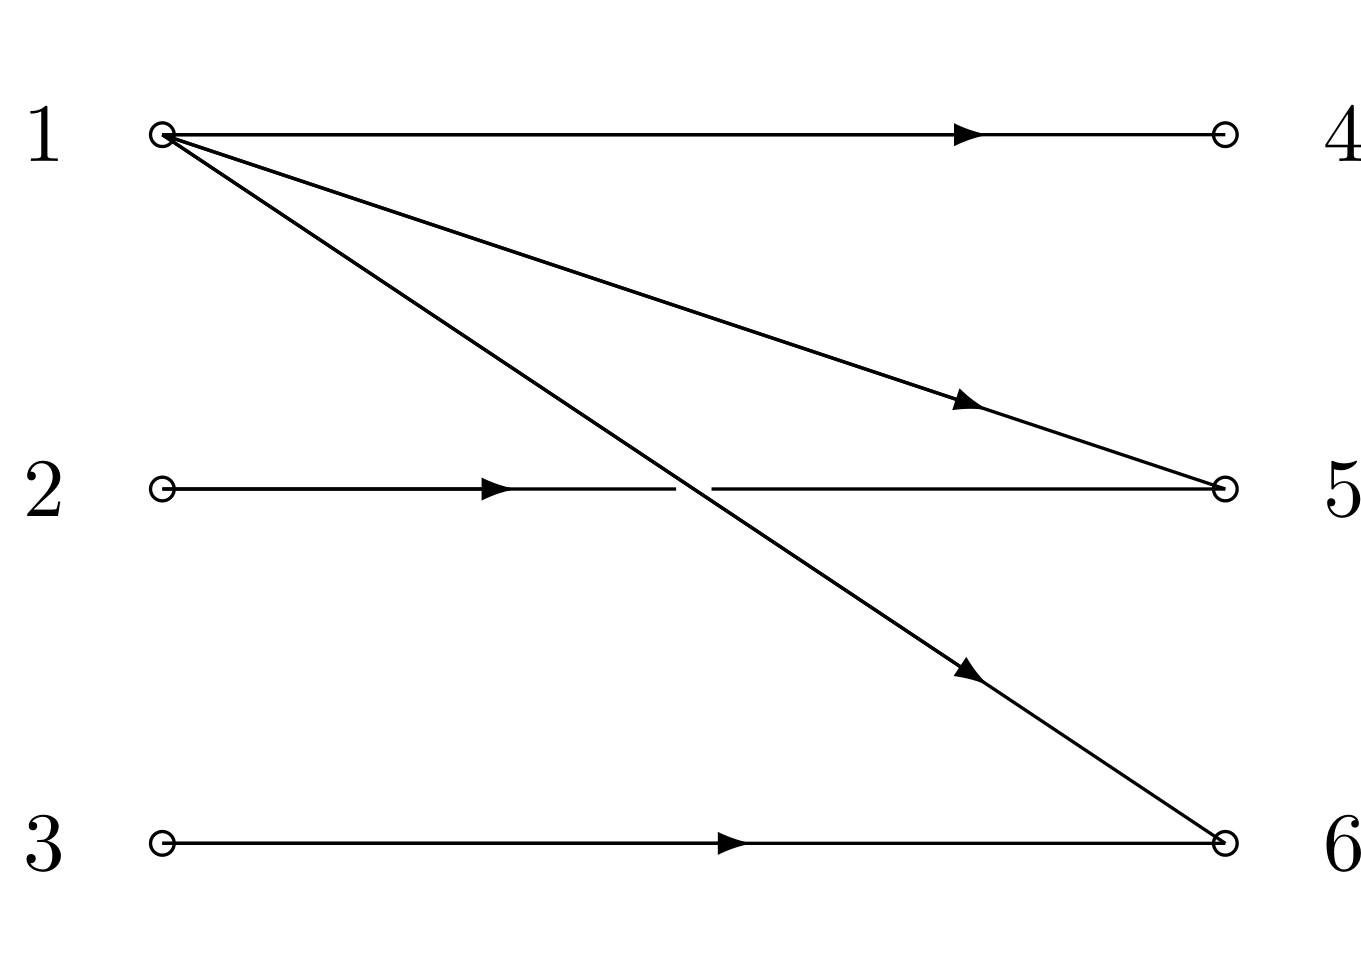
\includegraphics[width=5.76cm]{figures/fig-07.png}
  \caption{一个含 3 个源点与 3 个汇点的带标号有向树。\figorig{43}{7}}
  \label{fig:7}
\end{figure}

\subsection{有向树的计数}

Feynman 演算不仅可以用来计数无向图，也可以用来计数有向图。例如，假设我们要计数带标号的有向树，其顶点或为源点、或为汇点（见图 \ref{fig:7}）。此时容易看出（试检验之！），相应的积分问题是二维的，作用量为 $S=xy-be^x-ae^y$（形式 $xy$ 不是正定的，但这无关紧要，因为我们的计算是纯粹形式的）。于是临界点由方程
$$
xe^{-y}=a,\ ye^{-x}=b.
$$
求出。与前面一样，以下述形式寻找解 $(x,y)=(x_0,y_0)$：
$$
x=a+\sum_{p\ge 1,q\ge 1} c_{pq}a^pb^q,\ y=b+\sum_{p\ge 1,q\ge 1} d_{pq}a^pb^q.
$$
与无向树情形类似的计算（用留数）给出
$$
c_{pq}=\frac{1}{(2\pi i)^2}\oint\oint\frac{x}{a^{p+1}b^{q+1}}da\wedge db=
$$
$$
\frac{1}{(2\pi i)^2}\oint\oint \frac{e^{qx+py}}{x^py^{q+1}}(1-xy)dx\wedge dy=
\frac{q^{p-1}p^{q-1}}{(p-1)!q!}.
$$
类似地，$d_{pq}=\frac{q^{p-1}p^{q-1}}{p!(q-1)!}$。现在，与无向情形类似，可得 $-a\partial_aS(x,y)=x$，$-b\partial_bS(x,y)=y$，故
$$
-S(x,y)=b+\int_0^a\frac{x}{u}du=
a+b+\sum_{p,q\ge 1}\frac{p^{q-1}q^{p-1}}{p!q!}a^pb^q
$$
这表明带 $p$ 个源点与 $q$ 个汇点的带标号树的数目为 $p^{q-1}q^{p-1}\frac{(p+q)!}{p!q!}$。特别地，若指定哪些顶点为源点、哪些为汇点，则带标号树的数目为 $p^{q-1}q^{p-1}$。

\begin{exercise} 请详细完成这一计算。
\end{exercise}

\subsection{矩阵树定理}

这些计算可以推广，用以计算\emph{着色}带标号树的数目。为此，首先需要定义\emph{Kirchhoff 多项式} $K_m(\bold u)$。即：对一组变量 $\bold u:=(u_{ik})$，$1\le i\ne k\le m$，$u_{ik}=u_{ki}$，考虑二次型
$$
U(\bold y):=\sum_{1\le i<k\le m}u_{ik}(y_i-y_k)^2.
$$
一般地，它有由 $\bold 1=(1,...,1)$ 张成的一维核，因而在由方程 $\sum_i y_i=0$ 定义的子空间上非退化。该子空间带有一个体积形式 $\omega_0(v_1,...,v_{m-1}):=\omega(v_1,...,v_{m-1},\bold 1)$，其中 $\omega$ 是 $\Bbb R^m$ 上的标准体积形式；关于此形式有
$$
K_m(\bold u):=\det U=\det(\delta_{i\ell}\sum_{k\ne \ell} u_{k\ell }-u_{i\ell})_{(j)}
$$
对任意 $1\le j\le m$ 成立，其中下标 $(j)$ 表示删去第 $j$ 行与第 $j$ 列。多项式 $K_m$ 称为\emph{Kirchhoff 多项式}。例如 $K_2=u_{12}$，$K_3=u_{12}u_{13}+u_{13}u_{23}+u_{12}u_{23}$，等等。

现设 $\bold p=(p_1,...,p_m)$ 为正整数的 $m$ 元组，$\bold r=(r_{ij},1\le i\le j\le m)$ 为一组非负整数，满足 $|\bold r|=|\bold p|-1$，其中 $|\bold r|:=\sum_{i\le j}r_{ij}$，$|\bold p|:=\sum_k p_k$。设树的顶点被赋予颜色 $1,...,m$，而我们想计算带标号树的数目 $N(\bold p,\bold r)$：前 $p_1$ 个顶点染颜色 $1$，接下来的 $p_2$ 个染颜色 $2$，……，最后的 $p_m$ 个染颜色 $m$，且有 $r_{ij}$ 条边连接颜色 $i$ 的顶点与颜色 $j$ 的顶点。

只需计算多项式
$$
Q_{\bold p}(\bold z):=\sum_{\bold r: |\bold r|=|\bold p|-1} N(\bold p,\bold r)\prod_{i\le j}z_{ij}^{r_{ij}}. 
$$
\begin{theorem}\label{mt} 有
$$
Q_\bold p(\bold z)=
(p_1...p_m)^{-1}K(p_kz_{k\ell}p_\ell, k\ne \ell)\prod_\ell(\sum_k p_kz_{k\ell})^{p_\ell-1}.
$$
\end{theorem}

注意，当 $m=1$、$\bold z=1$ 时这恢复 Cayley 定理；而当 $m=2$、$\bold z=\begin{pmatrix} 0& 1\\ 1& 0\end{pmatrix}$ 时，它恢复我们对有向树的计数。

\begin{proof}
我们给每种颜色 $j$ 配一个实变量 $x_j$。则相应的作用量为
$$
S(x,y)=\frac{1}{2}x^TB x-\sum_{j=1}^m a_je^{x_j},
$$
其中 $B=(b_{ij})$ 是矩阵 $\bold z:=(z_{ij})$（$z_{ij}=z_{ji}$）的逆。于是由定理 \ref{trees1l}，$Q_{\bold p}(\bold z)$ 是 $-S(x)$ 中 $\prod_k a_k^{p_k}$ 的系数，其中 $x$ 是 $S$ 的临界点。

$S$ 的临界点方程为
$$
\sum_i x_ib_{ij}e^{-x_j}=a_j.
$$
令 $X_j:=\sum_i x_ib_{ij}$，则 $x_i=\sum_jz_{ij}X_j$，$a_i=X_ie^{-x_i}$，且对一切 $j$ 有
$$
-S(x)=\int X_j\frac{da_j}{a_j}
$$
换句话说，$-S(x)$ 中 $\prod_k a_k^{p_k}$ 的系数等于 $X_j(\bold z,\bold a)$ 中同一单项式的系数除以 $p_j$。因此，以 $D_T(\bold z)$ 记 $\bold z$ 对应于子集 $T\subset \lbrace 1,...,m\rbrace$ 的主子式，得到
$$
Q_{\bold p}(\bold z)=\tfrac{p_j^{-1}}{(2\pi i)^m}\oint X_j(\prod_k a_k^{-p_k-1})d\bold a=
$$
$$
\tfrac{p_j^{-1}}{(2\pi i)^m}\oint X_j(\prod_k (X_ke^{-x_k})^{-p_k-1})d(X_1e^{-x_1})\wedge...\wedge d(X_me^{-x_m})=
$$
$$
\tfrac{p_j^{-1}}{(2\pi i)^m}\oint \sum_{T\subset \lbrace 1,...,m\rbrace}(-1)^{|T|}D_T(\bold z)X_j(\prod_{\ell\notin T}X_\ell^{-1})(\prod_\ell X_\ell^{-p_\ell})e^{\sum_{k,\ell} p_kz_{k\ell}X_\ell}dX_1\wedge...\wedge dX_m
$$
$$
=p_j^{-1}\sum_{T\subset \lbrace 1,...,m\rbrace}(-1)^{|T|}\frac{p_j-1+\delta_{jT^c}}{\sum_k p_kz_{kj}}D_T(\bold z)\prod_\ell\frac{(\sum_k p_kz_{k\ell})^{p_\ell-\delta_{\ell T}}}{(p_\ell-\delta_{\ell T})!}=
$$
\scriptsize
$$
p_j^{-1}
\left(\frac{p_j-1}{\sum_k p_kz_{kj}}\det(\delta_{i\ell}\sum_k p_kz_{k\ell}-z_{i\ell}p_\ell)+
\det(\delta_{i\ell}\sum_k p_kz_{k\ell}-z_{i\ell}p_\ell)_{(j)}\right)\prod_\ell\frac{(\sum_k p_kz_{k\ell})^{p_\ell-1}}{p_\ell!},
$$
\normalsize
其中当 $\ell\in T$ 时 $\delta_{\ell T}=1$，否则为 $0$。第一个行列式为零，故得到
$$
Q_{\bold p}(\bold z)=(p_1...p_m)^{-1}\det(\delta_{i\ell}\sum_k p_kz_{k\ell}p_\ell-p_iz_{i\ell}p_\ell)_{(j)}\prod_\ell\frac{(\sum_k p_kz_{k\ell})^{p_\ell-1}}{p_\ell!}.
$$
这就蕴含定理。
\end{proof}

% [Tutor Note: “第一个行列式为零”这一步原文省略了理由：矩阵 M_{iℓ}=δ_{iℓ}·Σ_k p_k z_{kℓ} − z_{iℓ}p_ℓ 的第 i 行之和为 Σ_ℓ M_{iℓ}=Σ_k p_k z_{ki} − Σ_ℓ z_{iℓ}p_ℓ，而 z 对称（z_{iℓ}=z_{ℓi}）使两项相等，故每行之和为 0，det M=0。剩下的那个主子式正是加权矩阵树定理的“加权度−加权邻接”矩阵。另注意此处图论约定：z 是邻接矩阵的对称化（无自环，z_{ii} 不出现），Δ_Γ=D_Γ−A_Γ 取的是通常的（非负）Laplace 矩阵，故 U 半正定、核为一维常数向量；推论中的 1/m 因子正是来自“λ 中有一个零本征值”，即对 m−1 个非零本征值取积再除以 m。]

定理 \ref{mt} 是\emph{Kirchhoff 矩阵树定理}的加权版本，后者是 Cayley 定理的推广。更确切地说，取 $\bold z=A_\Gamma$ 为图 $\Gamma$（无自环）的邻接矩阵，$m$ 为 $\Gamma$ 的顶点数，并对一切 $i$ 取 $p_i=1$。则 $Q_{\bold p}(\bold z)=N_\Gamma$ 是 $\Gamma$ 的生成树的数目，而定理 \ref{mt} 断言
$$
N_\Gamma=\det U,
$$
其中 $U$ 是二次型
$$
U(\bold y)=\sum_{i<j}(A_\Gamma)_{ij}(y_i-y_j)^2=(\Delta_\Gamma \bold y,\bold y),
$$
其中 $\Delta_\Gamma=D_\Gamma-A_\Gamma$ 是 $\Gamma$ 的 Laplace 算子（$D_\Gamma$ 为顶点度数的对角矩阵）。于是得到

\begin{corollary} (矩阵树定理)
$$
N_\Gamma=\frac{1}{m}\lambda_1...\lambda_{m-1},
$$
其中 $\lambda_i$ 是 $\Delta_\Gamma$ 的非零本征值。
\end{corollary}

当 $\Gamma$ 是完全图时，由这一结果得到 Cayley 定理：此时对一切 $i$ 有 $\lambda_i=m$，故 $N_\Gamma=m^{m-2}$。

\subsection{单粒子不可约图与有效作用量}

设 $Z=Z_S$ 是对应于作用量 $S$ 的配分函数。在前几个小节中我们已经看到，量 $\hbar\log\frac{Z_S}{Z_0}$ 的“经典”（或“树”）部分 $(\log\frac{Z_S}{Z_0})_0$ 是相当初等的计算——它就是作用量 $S(x)$ 的临界值取负号。因此，若能找到一个新“有效”作用量 $S_{\rm eff}$（$S$ 的一个“形变”），使得
$$
\hbar^{-1}(\log\tfrac{Z_{\rm S_{\rm eff}}}{Z_0})_0=\log\tfrac{Z_S}{Z_0}
$$
（即有效作用量的经典答案就是原作用量的量子答案），则作用量 $S$ 的量子理论便可视为已解出。换句话说，求解附属于 $S$ 的量子理论（即求出相应的积分）的问题，本质上归结为计算有效作用量 $S_{\rm eff}$ 的问题。

下面我们给出用 Feynman 图振幅计算有效作用量的方法，并将看到它在计算上比求连通图之和更容易。

\begin{definition}
设 $e$ 是连通图 $\Gamma$ 的一条边。若图 $\Gamma\setminus\ e$ 不连通，则称该边为\emph{桥}。不含桥的连通图称为\emph{单粒子不可约}（1PI）的。\footnote{这是物理术语；数学术语为“2-连通”。}
\end{definition}

为计算有效作用量，我们需要考虑带外线的图（但至少含一个内顶点）。这样的图 $\Gamma$（带 $N$ 条外线）称为单粒子不可约的，如果相应的“截肢”图（即从 $\Gamma$ 中删去外线所得的图）是单粒子不可约的。特别地，含一个内顶点的图总是单粒子不可约的；而无内顶点的单边图则\emph{不}定义为单粒子不可约。桥与单粒子不可约图的概念见图 \ref{fig:8}。

\begin{figure}[htbp]
  \centering
  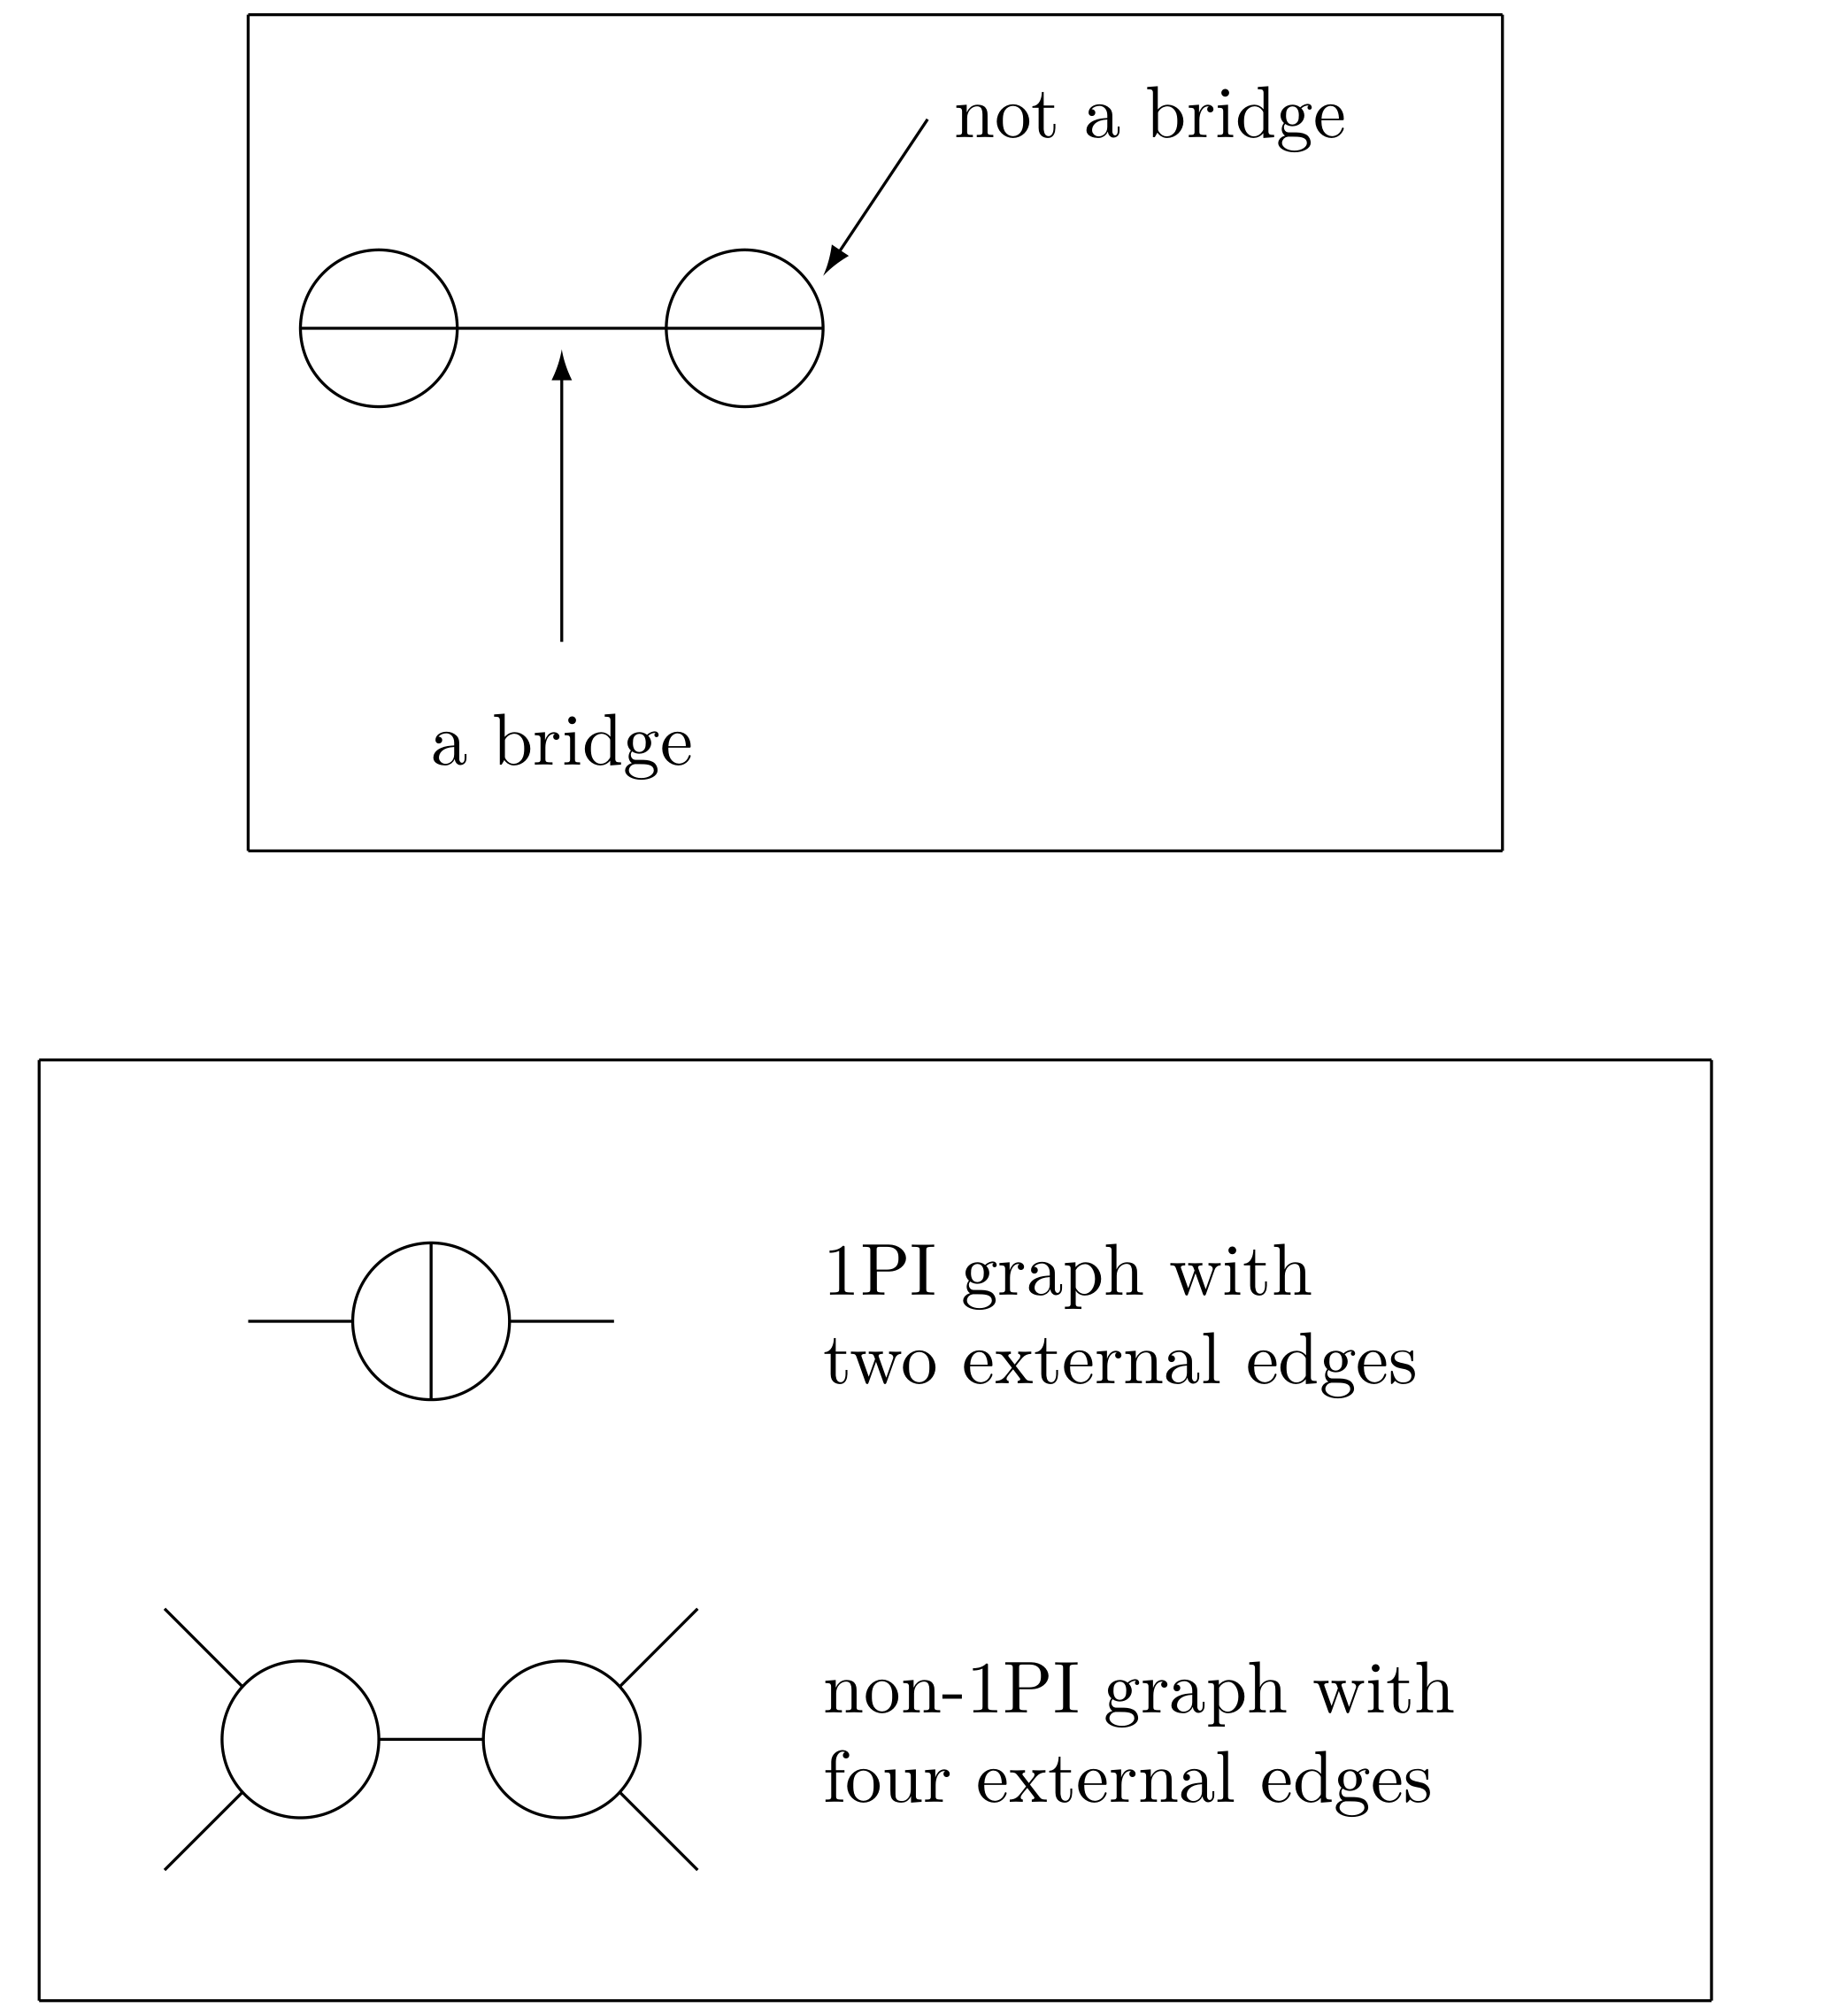
\includegraphics[width=8.76cm]{figures/fig-08.png}
  \caption{（原文无图题）\figorig{47}{8}}
  \label{fig:8}
\end{figure}

用 $G_{\rm 1PI}(\bold n,N)$ 表示如下单粒子不可约图的同构类的集合：它们有 $N$ 条外线，且对每个 $i$ 有 $n_i$ 个 $i$ 价内顶点（这里同构不允许移动外线）。

\begin{theorem} \label{effac}
有效作用量 $S_{\rm eff}$ 由公式
$$
S_{\rm eff}(x)=
 \frac{B(x,x)}{2}-
\sum_{i\ge 0}\frac{{\mathcal B}_i(x,...,x)}{i!},
$$
给出，其中
$$
{\mathcal B}_N(x, \ldots ,x)=\hbar\sum_{\bold n}\prod_i (g_i\hbar^{\frac{i}{2}-1})^{n_i}
\sum_{\Gamma\in G_{\rm 1PI}(\bold
  n,N)}\frac{\Bbb F_\Gamma(Bx, \ldots ,Bx)}{|{\rm Aut}(\Gamma)|}.
$$
\end{theorem}

% [Tutor Note: 这里的 ℏ 幂次是“圈数记账”，最易算错。对带 N 条外线、n_i 个 i 价内顶点的 1PI 图，由欧拉公式其圈数为 L=1−N/2+Σ_i n_i(i/2−1)；正文中每个内顶点配权 g_iℏ^{i/2−1}、每个外线顶点（对应 Bx）不配 ℏ，再把整个 B_N 乘一个 ℏ，正好给出 ℏ^{1+Σ n_i(i/2−1)}。由于外部 Bx 已吸收 B 的指标结构，这就是 Feynman 规则中“顶点权 g_i”在 ℏ 展开下的自然权重；据此 S_eff=S+ℏS_1+ℏ²S_2+… 中 ℏ^j S_j 即 j 圈修正。]

于是 $S_{\rm eff}=S+\hbar S_1+\hbar^2 S_2+..$。诸表达式 $\hbar^j S_j$ 称为有效作用量的\emph{$j$ 圈修正}。

该定理使物理学家只需处理单粒子不可约图，这也是读者很少在 QFT 教科书中见到其他图的原因。与前面一样，它在低阶计算中非常有用，因为给定圈数的单粒子不可约图的数目远小于同圈数的连通图的数目。

\begin{proof} 证明基于图论中下述引理。

\begin{lemma}\label{obv} 任意连通图 $\Gamma$ 都可唯一地表示为一棵树，其顶点是（带外线的）单粒子不可约子图，其边是 $\Gamma$ 的桥。
\end{lemma}

该引理是显然的。即，从 $\Gamma$ 中删去所有桥，则 $\Gamma$ 变成一些单粒子不可约图的不交并，这些图即取作上述树的顶点。

对应于图 $\Gamma$ 的这棵树称为 $\Gamma$ 的\emph{骨架}（见图 \ref{fig:9}）。

\begin{figure}[htbp]
  \centering
  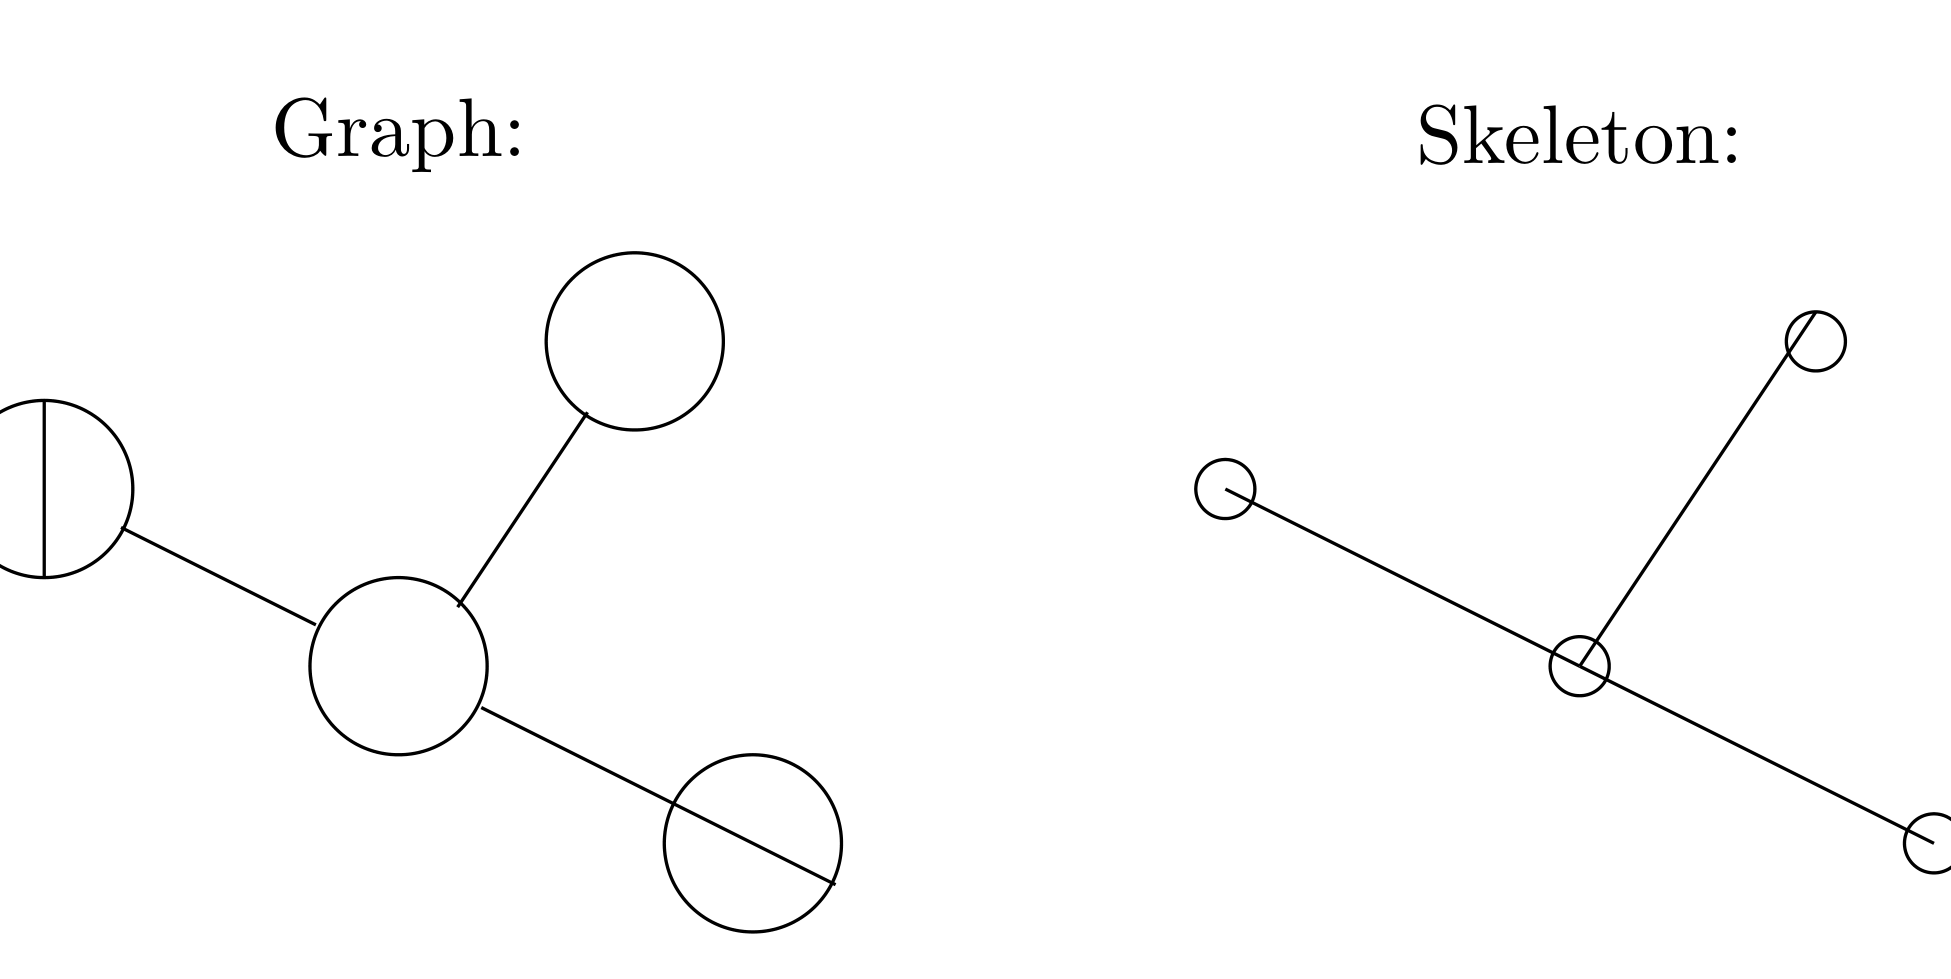
\includegraphics[width=8.26cm]{figures/fig-09.png}
  \caption{一个图的骨架。\figorig{49}{9}}
  \label{fig:9}
\end{figure}

容易看出引理 \ref{obv} 蕴含定理 \ref{effac}。事实上，它表明在 $\log\frac{Z_S}{Z_0}$ 的表达式中出现的所有连通图之和可以写成对骨架树的求和，于是每棵树的贡献（正比于）放在其顶点上的张量 ${\mathcal B}_i$ 的缩并，而 ${\mathcal B}_i$ 是所有带 $i$ 条外线的单粒子不可约图的振幅的（加权）和。
\end{proof}

\subsection{单粒子不可约图与 Legendre 变换}

回忆\emph{Legendre 变换}的概念。设 $f$ 是向量空间 $Y$ 上的光滑函数，使得由 $x\to df(x)$ 给出的映射 $Y\to Y^*$ 是微分同胚。则可如下定义 $f$ 的 Legendre 变换：对 $p\in Y^*$，设 $x_0=x_0(p)$ 是函数 $(p,x)-f(x)$ 的临界点（即方程 $df(x)=p$ 的唯一解），则 $f$ 的 Legendre 变换是由
$$
L(f)(p)=(p,x_0)-f(x_0).
$$
定义的 $Y^*$ 上的函数。容易看出 $L(f)$ 的微分也是微分同胚 $Y^*\to Y$（事实上是 $df(x)$ 的逆），且 $L^2(f)=f$。

\begin{example} 设 $f(x)=\frac{ax^2}{2}$，$a\ne 0$。则 $px-f=px-\frac{x^2}{2}$ 在 $p=\frac{x}{a}$ 处有临界点，临界值为 $\frac{p^2}{2a}$。于是 $L(\frac{ax^2}{2})=\frac{p^2}{2a}$。更一般地，若 $f(x)=\frac{B(x,x)}{2}$，其中 $B$ 是 $Y$ 上的非退化对称形式，则 $L(f)(p)=\frac{B^{-1}(p,p)}{2}$。例如，质量为 $m$ 的粒子其拉格朗日量 $\frac{mv^2}{2}-U(x)$ 关于速度 $v=\dot{x}$ 的 Legendre 变换就是它的哈密顿量（能量）$\frac{p^2}{2m}+U(x)$，反之亦然。事实上，这一点在完全一般的情形下都成立，这正是 Legendre 变换在经典力学与场论中起重要作用的原因。
\end{example}

注意，驻相公式表明 Legendre 变换是 Fourier 变换的经典类比。事实上，Feynman 密度 $e^{\frac{iS(x)}{\hbar}}dx$ 的（适当归一化的）Fourier 变换 $\hbar^{-\frac{d}{2}}\int_V e^{\frac{i(-(p,x)+S(x))}{\hbar}}dx$（其中积分按分布的意义理解）取对数后，当 $\hbar\to 0$ 时的渐近展开的首项为 $-\frac{iL(S)(p)}{\hbar}$。

现在我们在定理 \ref{Feyn} 的情形下考察定理 \ref{effac}。于是 $S(x)=\frac{B(x,x)}{2}+O(x^3)$，我们考察
$$
Z(p)=\hbar^{-\frac{d}{2}}\int_Ve^{\frac{(p,x)-S(x)}{\hbar}}dx.
$$
由定理 \ref{effac}，有
$$
\log\frac{Z(p)}{Z_0}=-\hbar^{-1}S_{\rm eff}(x_0,p),
$$
其中有效作用量 $S_{\rm eff}(x,p)$ 是对单粒子不可约图的求和，而 $x_0=x_0(p)$ 是它的临界点。

现在必须有 $S_{\rm eff}(x,p)=-p\cdot x+S_{\rm eff}(x)$，因为唯一含 1 价内顶点（对应于 $p$）的 1PI 图就是只有一条边的图：它把一个内顶点与一个外顶点相连（故给出项 $-p\cdot x$，而其他图不含 $p$ 顶点）。这表明 $\hbar\log\frac{Z(p)}{Z_0}$ 是 $p\cdot x-S_{\rm eff}(x)$ 的临界值。于是我们证明了以下结论。

\begin{proposition} 有
$$
S_{\rm eff}(x)=L(\hbar\log\tfrac{Z(p)}{Z_0}),\ \hbar\log\tfrac{Z(p)}{Z_0}=L(S_{\rm eff}(x)).
$$
\end{proposition}

物理学家将该结果表述如下：有效作用量是 $\hbar$ 乘以量子关联函数生成函数之对数的 Legendre 变换（反之亦然）。

\begin{exercise} 计算
$$
S(x)=\tfrac{x^2}{2}-g(x+\tfrac{x^3}{6}).
$$
的 $\log\frac{Z}{Z_0}$ 的一圈贡献。利用此结果，计算只含 1 价与 3 价顶点的、带 n 个顶点的带标号一圈图的数目（注意重边与自环！）。通过直接枚举顶点数较少的这类图来检验你的答案。
\end{exercise}

\begin{exercise}
求只含 1 价与 4 价顶点的带 n 个顶点的带标号树的数目 $a_n$ 的指数生成函数 $\sum_n a_n\frac{z^n}{n!}$。答案可以用多项式的反函数表示。
\end{exercise}

\begin{exercise} 求 $S(x)=\frac{x^2}{2}-\frac{gx^3}{6}$ 的有效作用量的一圈贡献。即，有 $S_{\rm eff}=S+\hbar S_1+O(\hbar^2)$，需要求出 $S_1$。需要考虑哪些 Feynman 图？
\end{exercise}

\begin{exercise} 考虑热方程 $u_t=\frac{1}{2}\Delta_B u$，其中 $\Delta_B$ 是第 \ref{inse} 小节中定义的附属于 $B$ 的 Laplace 算子。它由热流 $u(x,t)=e^{\frac{t\Delta_B}{2}}u(x,0)$ 解出。证明：作用量 $S(x)=\frac{B(x,x)}{2}-\widetilde S(x)$ 的有效作用量 $S_{\rm eff}$ 可以计算为作用量 $S^\circ(x):=\frac{B(x,x)}{2}-\widetilde S^\circ(x)$ 的无自环 1PI Feynman 图贡献之和，其中 $\widetilde S^\circ(x):=e^{\frac{\hbar\Delta_B}{2}}\widetilde S(x)$ 是用时间为 $\hbar$ 的热流变换 $\widetilde S$ 所得。
\end{exercise}

\bigskip
\noindent\rule{\textwidth}{0.6pt}
% [Tutor Note: 本章小结——§3.7–3.12 把“树”当作组合骨架：临界点方程的不动点迭代给出树展开，Cayley 定理与加权矩阵树定理是它在 d=1、完全图与着色情形下的特例；§3.13–3.14 把同一骨架提升到量子层面：把连通图按桥收缩成以 1PI 子图为顶点的骨架树，得到有效作用量的圈展开，其经典（树）部分恰为原作用量临界值取负。最易出错处有两点：一是 Legendre 变换的符号与变量——原文定义 L(f)(p)=(p,x_0)-f(x_0) 以 p 为自变量，故命题写成 S_eff(x)=L(ℏ log(Z/Z_0))；文献中常写成 Γ[φ]=sup_J(Jφ-W[J])，两者只差 W 的整体符号约定，务必沿途跟踪。二是 L²(f)=f 只在临界点唯一（凸性）时成立，多临界点处只能逐分支谈论，量子修正下更要小心。]


%=====================================================================
% 4  矩阵积分
% 原文：Section 4. Matrix integrals（arXiv:2409.03117v1, p. 51--62）
%=====================================================================
\section{矩阵积分}

\begin{keytakeaways}
\begin{itemize}
  \item \textbf{物理图像：}矩阵积分把随机矩阵的谱理论与二维曲面的组合拓扑统一起来。对大 $N$，配分函数对数关于耦合常数的展开按胖图（即带边曲面）的亏格分层，每一项都携带因子 $N^{2-2{\rm g}}$，而 $2-2{\rm g}$ 正是亏格 ${\rm g}$ 的闭曲面的欧拉示性数。
  \item \textbf{数学工具：}Feynman 定理加张量缩并：把每个 $i$-价花加胖，再沿匹配保向粘合，缩并给出 $\widetilde{\Bbb F}(\sigma)=N^{\nu(\widetilde\Gamma_\sigma)}$，即边界分支数 $\nu$ 成为 $N$ 的幂次；再由欧拉公式 $b=2{\rm g}-2+\nu$ 与标度变换 $\hbar\mapsto\hbar/N$ 即得亏格展开。
  \item \textbf{关键结论：}'t Hooft 定理：极限 $W_\infty=\lim_{N\to\infty}N^{-2}\log\widehat Z_N$ 由亏格零的平面胖图支配；而 $\log\widehat Z_N/N^2$ 按 $N^{-2{\rm g}}$ 的展开，其第 ${\rm g}$ 阶恰由亏格 ${\rm g}$ 的连通曲面贡献。实对称矩阵情形允许带子扭转 $180^\circ$ 的粘合，此时亏格可取半整数。
  \item \textbf{易错点：}作用量中 $\Tr(A^m)$ 的系数是 $1/m$ 而非 $1/m!$；Wigner 半圆律的第 $2m$ 阶矩等于 Catalan 数 $C_m$；Hermite 多项式按权 $e^{-x^2}$（而非 $e^{-x^2/2}$）正交，其范数平方为 $2^nn!\sqrt{\pi}$。
\end{itemize}
\end{keytakeaways}

\bigskip
\noindent\rule{\textwidth}{0.6pt}
\bigskip

设 ${\frak h}_N$ 为 $N$ 阶 Hermitian 矩阵所成空间。${\frak h}_N$ 上的内积由 $B(A_1,A_2)=\Tr(A_1A_2)$ 给出。本节考虑如下形式的积分：
$$
Z_N:=\hbar^{-\frac{N^2}{2}}\int_{{\frak h}_N}e^{-\frac{S(A)}{\hbar}}dA,
$$
其中 Lebesgue 测度 $dA$ 按条件
$$
\int_{{\frak h}_N} e^{-\frac{{\rm Tr}(A^2)}{2}}dA=1
$$ 
归一化（这样就不必处处携带 $\sqrt{2\pi}$ 因子），而
$$
S(A):=\frac{\Tr(A^2)}{2}-\sum_{m\ge 1} g_m\frac{\Tr(A^m)}{m}
$$
是作用量泛函。\footnote{注意这里除以 $m$ 而不是 $m!$。下文将说明这种归一化为何更为方便。} 我们关心的是 $Z_N$ 关于 $g_i$ 的展开系数在大 $N$ 时的行为。对这一行为的研究将引导我们不去考虑简单的 Feynman 图，而是考虑胖图（或带状图）——它们实际上是二维曲面。因此，在进一步推进之前，我们需要做一些二维组合拓扑。
% [Tutor Note: 原文脚注强调作用量里除以 m 而非 m!，这一点决定了全部组合因子。由 B_m=(m-1)!\Tr(A^m) 以及 Feynman 定理，每个 i 价花给出 (i-1)! 而非 i!；而 log Z_N 的展开式中已带 1/i^{n_i}n_i!，再对每个花的循环次序 S_{i-1} 求和给出 (i-1)! 倍，二者相抵后分母只剩 i^{n_i}n_i!。核对顶点系数时切勿再补一个 1/i!；这也是后文把 \prod_i i!^{n_i} 换成 \prod_i i^{n_i} 的来源。]

\subsection{胖图}
回想 Feynman 定理的证明：给定有限个花（flower）以及在其各边端点所成集合 $T$ 上的一个匹配 $\sigma$，把落在同一对中的点连接（粘合）起来，便得到图 $\Gamma_\sigma$。

现在，给定一个 $i$-价花，把它内接于一个闭圆盘 $D$（使各边的端点都落在边界上），再在 $D$ 中取它的一小块管状邻域。这样就得到一个边界分段光滑的区域。我们为该区域及其边界取标准定向，并称之为一个\emph{胖 i-价花}。一个胖 $i$-价花的边界形如 $P_1Q_1P_2Q_2 \ldots P_iQ_iP_1$，其中 $P_i,Q_i$ 为角点，区间 $P_jQ_j$ 是 $\partial D$ 上的弧，而 $Q_jP_{j+1}$ 是位于 $D$ 内部的（光滑）弧（见图~\ref{fig:10}）。

\begin{figure}[htbp]
  \centering
  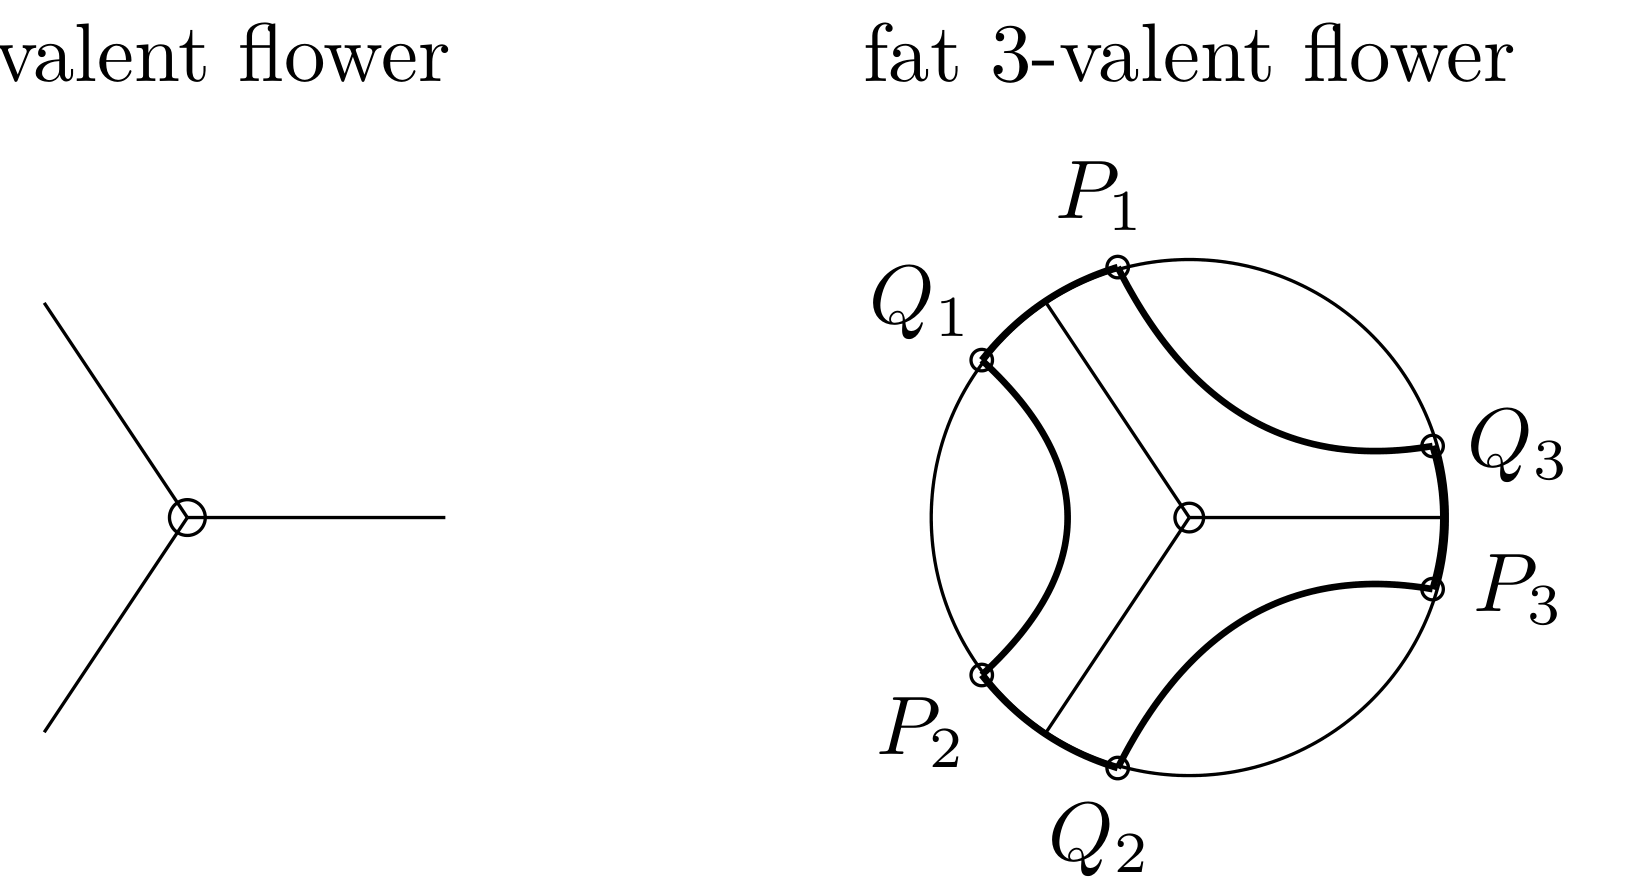
\includegraphics[width=6.92cm]{figures/fig-10.png}
  \caption{（原文无图题）\figorig{52}{10}}
  \label{fig:10}
\end{figure}


现在，给定一族通常的花以及如上所述的一个匹配 $\sigma$，我们取相应的胖花，并按 $\sigma$ 沿区间 $P_jQ_j$ 保向地粘合它们。这将产生一个带边的紧定向曲面（其边界由区间 $Q_{j}P_{j+1}$ 粘合而成）。我们用 $\widetilde \Gamma_{\sigma}$ 记这个曲面，并称之为 $\Gamma$ 关于 $\sigma$ 的\emph{加胖}。图的加胖称为\emph{胖图}（或\emph{带状图}）。

因此，胖图并不只是一个带边的定向曲面，而是这样的曲面连同把它分割成胖花的一个划分。

注意同一个图 $\Gamma$ 可以有许多互不同胚（尽管同伦等价）的加胖，特别地，加胖的亏格 ${\rm g}$ 并\emph{不}由 $\Gamma$ 决定（见图~\ref{fig:11}）。

\begin{figure}[htbp]
  \centering
  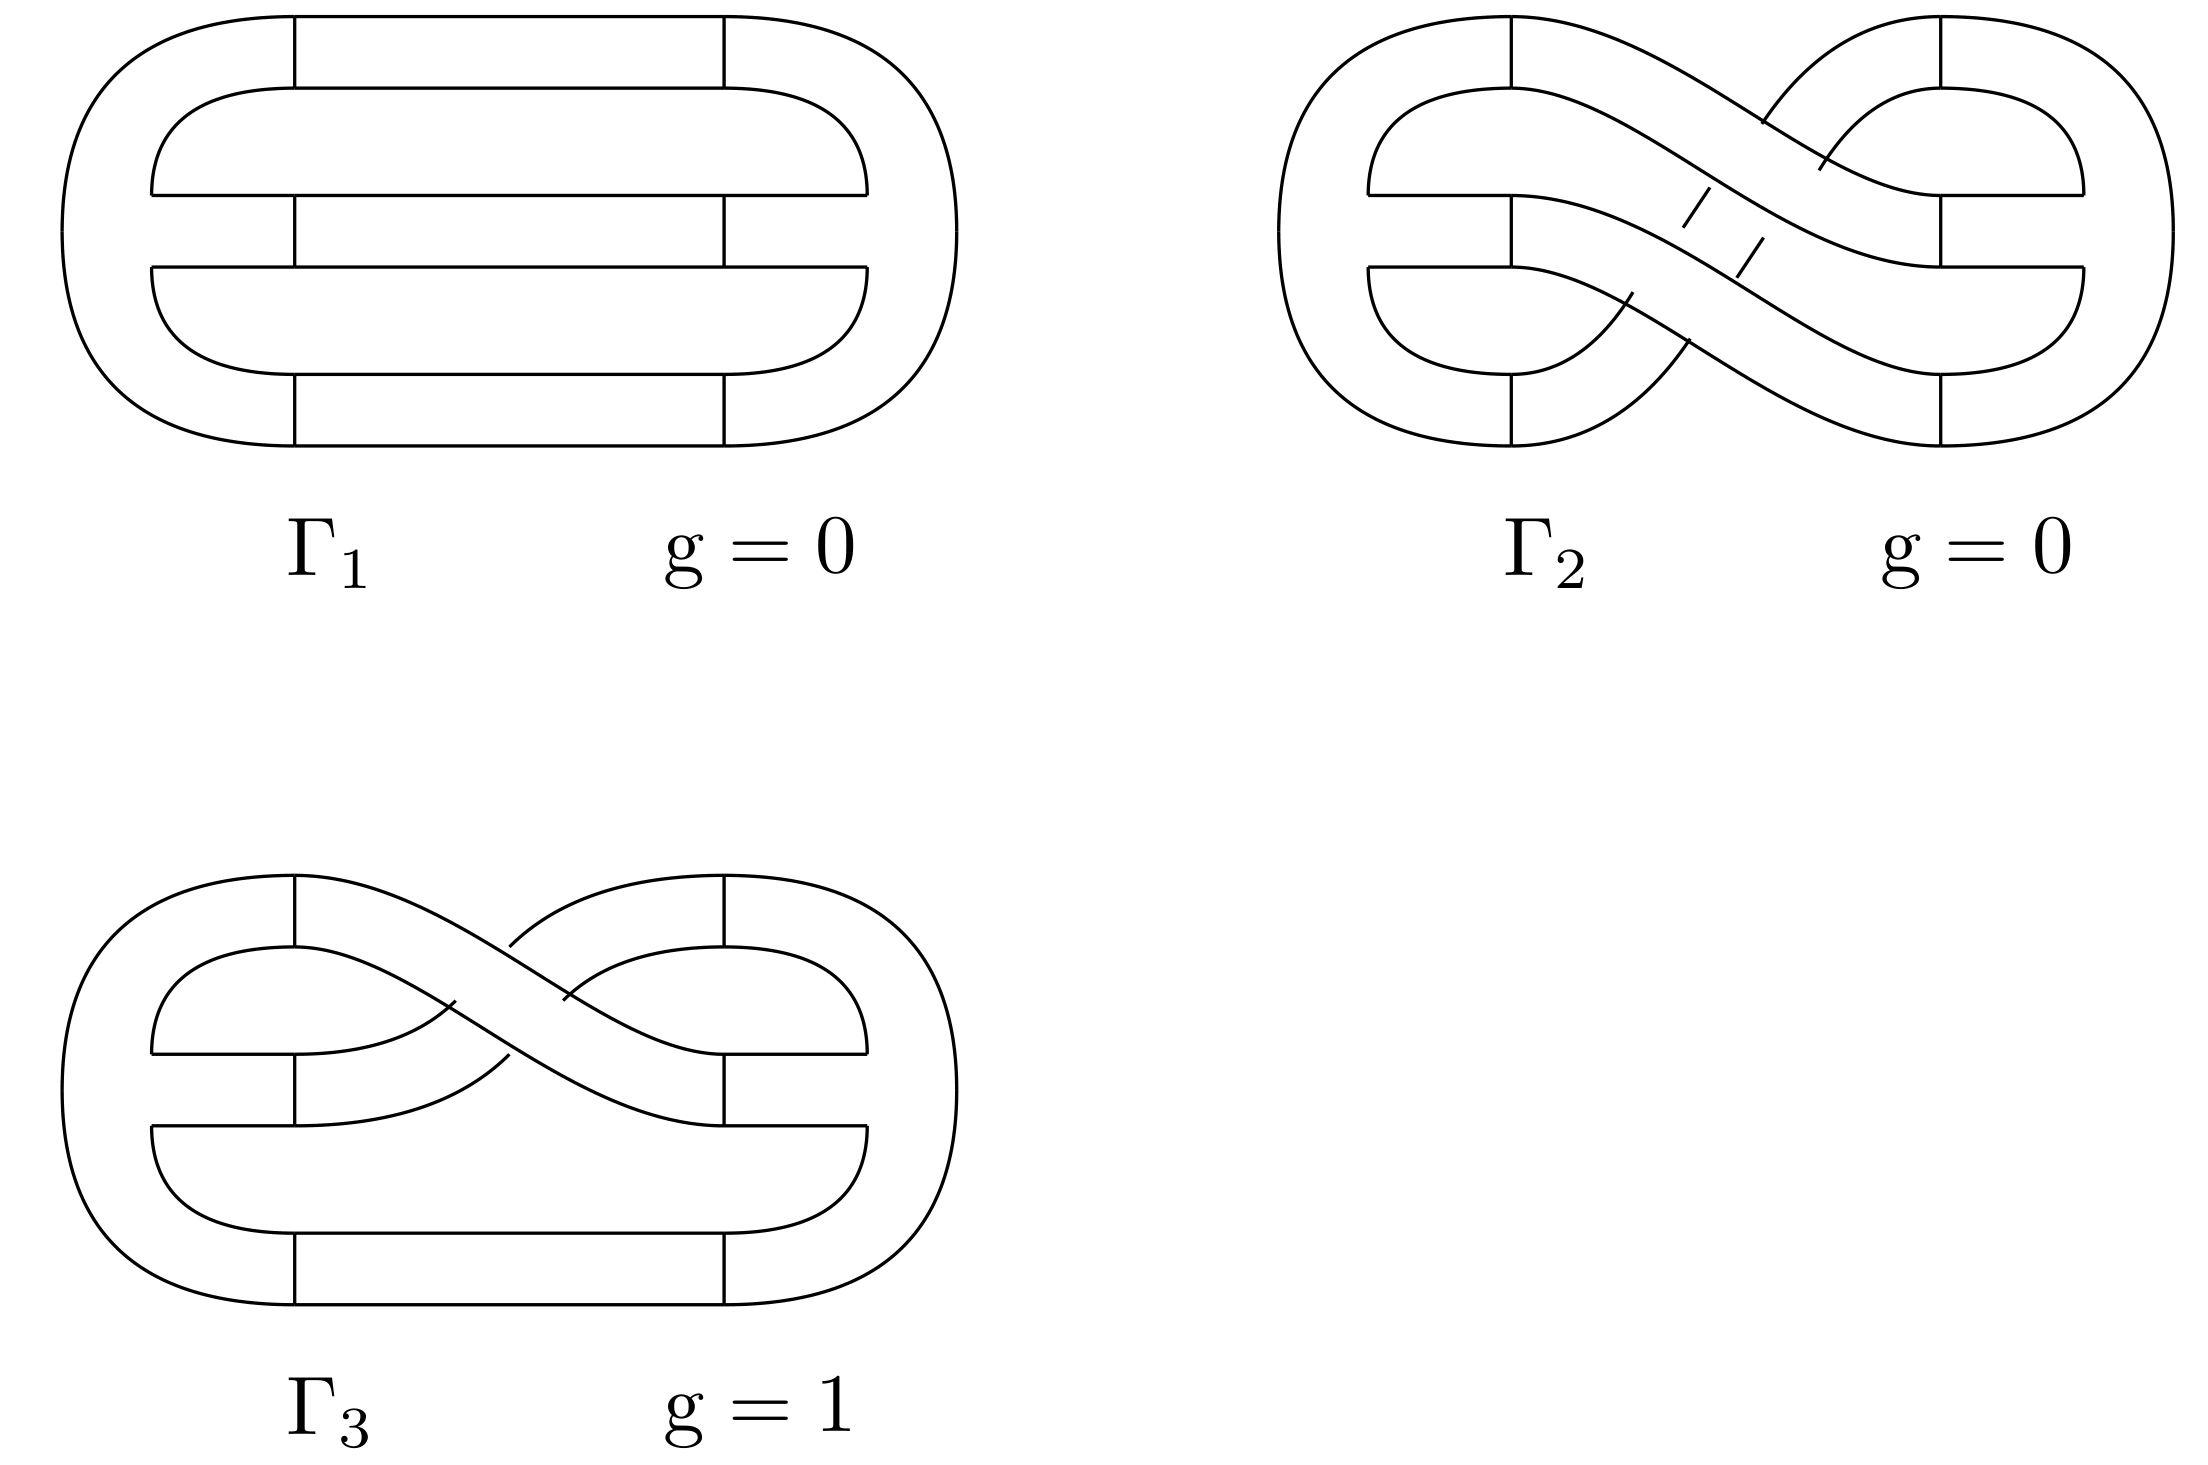
\includegraphics[width=9.35cm]{figures/fig-11.png}
  \caption{由胖花粘合胖图\figorig{52}{11}}
  \label{fig:11}
\end{figure}

\subsection{大 $N$ 极限中的矩阵积分、平面图与亏格展开}

现在回到积分 $Z_N$ 的研究。我们有
$$
B_m(A,...,A)=(m-1)!\Tr(A^m).
$$ 
于是由 Feynman 定理，
$$
\log Z_N=\sum_{\bold n}\prod_i \frac{(g_i\hbar^{\frac{i}{2}-1})^{n_i}}{i!^{n_i}n_i!}
\sum_{\sigma\in \Pi_c(T_{\bold n})}\Bbb F(\sigma),
$$
其中求和遍历集合 $\Pi_c(T_{\bold n})$——即 $T=T_{\bold n}$ 的所有使图 $\Gamma_\sigma$ 连通的匹配，而 $\Bbb F(\sigma)$ 表示用 $\sigma$ 对张量 $(m-1)!\Tr(A^m)$ 作缩并的结果。下面来计算 $\Bbb F(\sigma)$。

设 $\lbrace e_i\rbrace$ 是 $\Bbb C^N$ 的标准基，$\lbrace e_i^*\rbrace$ 是对偶空间中的对偶基。则张量 $\Tr(A^m)$ 可以写成
$$
\Tr(A^m)=\sum_{i_1, \ldots ,i_m=1}^N
(e_{i_1}\otimes e_{i_2}^*\otimes e_{i_2}\otimes e_{i_3}^*\otimes \cdots
\otimes e_{i_m}\otimes e_{i_1}^*,A^{\otimes m}).
$$
因此
$$
B_m=\sum_{s\in S_{m-1}}\sum_{i_1, \ldots ,i_m=1}^N
s(e_{i_1}\otimes e_{i_2}^*\otimes e_{i_2}\otimes e_{i_3}^*\otimes \cdots
\otimes e_{i_m}\otimes e_{i_1}^*)
$$
（对 $m$-价花各边的所有可能的循环次序求和）。于是
$$
\Bbb F(\sigma)=\sum_{s\in \prod_i S_{i-1}^{n_i}} \widetilde {\Bbb F}(s\sigma),
$$
其中 $\widetilde {\Bbb F}(\sigma)$ 是按胖图 $\widetilde\Gamma_{\sigma}$ 缩并张量
\begin{equation}\label{tenso}
\sum_{i_1,...,i_m=1}^Ne_{i_1}\otimes e_{i_2}^*\otimes e_{i_2}\otimes e_{i_3}^*\otimes \cdots
\otimes e_{i_m}\otimes e_{i_1}^*
\end{equation} 
所得的结果。由此可得
$$
\log Z_N=
\sum_{\bold n}\prod_i \frac{g_i^{n_i}\hbar^{n_i(\frac{i}{2}-1)}}{i!^{n_i}n_i!}
\sum_{\sigma\in \Pi(T_{\bold n})}\sum_{s\in \prod_i S_{i-1}^{n_i}}\widetilde {\Bbb F}(s\sigma)=
$$
$$
\sum_{\bold n}\prod_i \frac{g_i^{n_i}\hbar^{n_i(\frac{i}{2}-1)}}{i^{n_i}n_i!}
\sum_{\sigma}\widetilde {\Bbb F}(\sigma)
$$
（分母中的 $\prod_i i!^{n_i}$ 被换成了 $\prod_i i^{n_i}$，因为在和 $\sum_{s,\sigma}\widetilde {\Bbb F}(s\sigma)$ 中，每一项 $\widetilde {\Bbb F}(\sigma)$ 都出现 $|\prod_i S_{i-1}^{n_i}|=\prod_i (i-1)!^{n_i}$ 次）。

对带边曲面 $\Sigma$，用 $\nu(\Sigma)$ 表示其边界连通分支的个数。

\begin{proposition}\label{fatt}
$\widetilde {\Bbb F}(\sigma)=N^{\nu(\widetilde\Gamma_{\sigma})}$.
\end{proposition}

\begin{proof}
可以把和 \eqref{tenso} 中的每一项看成用 $i_1,i_2,i_2,i_3, \ldots ,i_m,i_1$ 对胖 $m$-价花边界上的角点 $P_1,Q_1, \ldots ,P_m,Q_m$ 所作的一种标号。现在，用 $\sigma$ 对某一组这样的单项式作缩并，其结果非零当且仅当下标沿着 $\widetilde\Gamma_{\sigma}$ 的每个边界分支都是常数（见图 12）。由此即得结论。
\end{proof}

\begin{figure}[htbp]
  \centering
  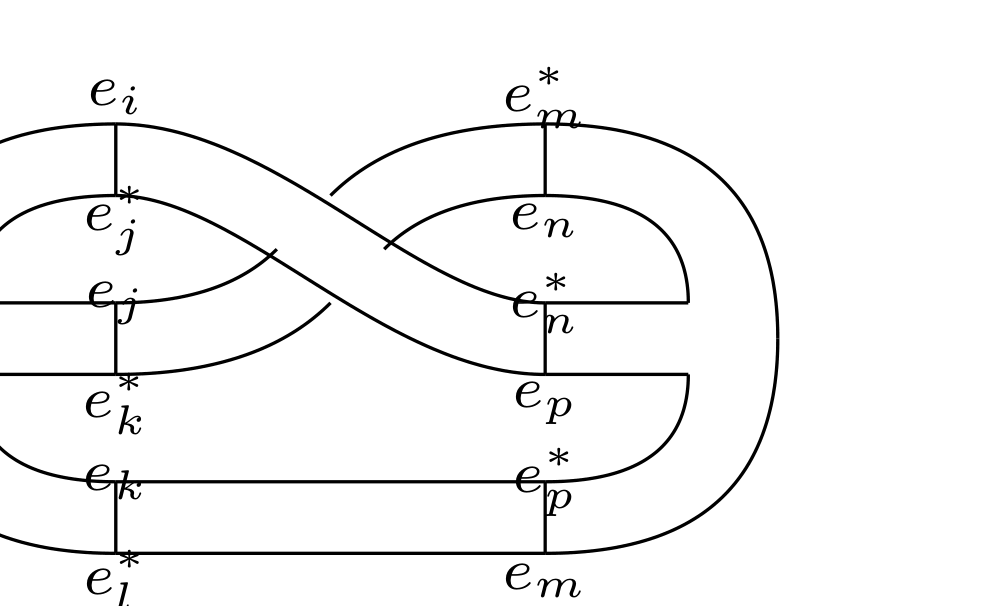
\includegraphics[width=4.2cm]{figures/fig-12.png}
  \caption{由胖图定义的缩并。\figorig{54}{12}}
  \label{fig:12}
\end{figure}

设 $\widetilde G_c(\bold n)$ 是连通胖图的同构类所成集合，其中对每个 $i\ge 1$ 恰有 $n_i$ 个 $i$-价顶点。对 $\widetilde\Gamma\in \widetilde G_c(\bold n)$，用 $b(\widetilde\Gamma)$ 表示其底层的通常图 $\Gamma$ 的边数减去顶点数。

\begin{corollary}\label{fatt1}
$$
\log Z_N=\sum_{\bold n}\prod_i (g_i\hbar^{\frac{i}{2}-1})^{n_i}
\sum_{\widetilde\Gamma\in \widetilde G_c(\bold n)}\frac{N^{\nu(\widetilde\Gamma)}}
{|{\rm Aut}(\widetilde\Gamma)|}=
$$
$$
\sum_{\bold n}\prod_i g_i^{n_i}
\sum_{\widetilde\Gamma\in \widetilde G_c(\bold n)}\frac{N^{\nu(\widetilde\Gamma)}\hbar^{b(\widetilde\Gamma)}}
{|{\rm Aut}(\widetilde\Gamma)|}.
$$
\end{corollary}

\begin{proof} 
令 $\Bbb G_{\bold n}^{\rm cyc}:=
\prod_i (S_{n_i}\ltimes (\Bbb Z/i\Bbb Z)^{n_i})$。
此群作用在 $T_{\bold n}$ 上，使得对任意 $g\in \Bbb G_{\bold n}^{\rm cyc}$ 都有
$\widetilde\Gamma_{\sigma}=\widetilde\Gamma_{g\sigma}$。
此外，该群在给出同一个胖图 $\widetilde\Gamma_{\sigma}$ 的所有 $\sigma$ 之集上可迁地作用，并且任一 $\sigma$ 的稳定子恰为
${\rm Aut}(\widetilde\Gamma_{\sigma})$。由此即得结论，因为 $|\Bbb G_{\bold n}^{\rm cyc}|=\prod_i i^{n_i}n_i!$ 
正好消去各分母。
\end{proof}
% [Tutor Note: 对称因子 |Aut(\widetilde\Gamma)| 此处是“保胖花结构的图自同构”，不是底层的普通图自同构：它包含每个花上循环次序的旋转（(Z/iZ)^{n_i}）。群 \Bbb G_{\bold n}^{\rm cyc} 的阶 \prod_i i^{n_i}n_i! 与 Feynman 展开的分母相消，剩下 1/|Aut|，这正是 Burnside 式的计数；用组合方法直接数胖图时容易把旋转对称漏掉或因重复计数而多除，务必核对。]

现在，对任意带边的紧连通曲面 $\Sigma$，用 ${\rm g}(\Sigma)$ 表示 $\Sigma$ 的亏格。则对连通胖图
$\widetilde\Gamma$，
$$
b(\widetilde\Gamma)=
2{\rm g}(\widetilde\Gamma)-2+\nu(\widetilde\Gamma)
$$ 
（即负的欧拉示性数）。于是若定义
$$
\widehat Z_N(\hbar):=Z_N(\tfrac{\hbar}{N}),
$$
便得到
% [Tutor Note: 从推论 4.2 到定理 4.3 的关键一步是把 \hbar 标度为 \hbar/N 并用 \nu-b=2-2g。明细如下：推论中每项为 g_i^{n_i}N^{\nu}\hbar^{b}，把 \hbar 换成 \hbar/N 得到 N^{\nu-b}\hbar^{b}；又由欧拉公式 b=2g-2+\nu 得 \nu-b=2-2g。于是 N 的幂次只剩 2-2g，而 \hbar 的幂次 b 恰好等于 \prod_i(i/2-1)n_i=\frac12\sum i n_i-\sum n_i（后者用了边数 E=\frac12\sum i n_i）。核对任意给定图的 N 幂次时，先数边界分支 \nu 与 b=E-V，再算 \nu-b 最稳妥。实对称（扭转）情形公式形式不变，但 g=1-\chi/2 可取半整数（RP^2：\chi=1 故 g=1/2；Klein 瓶：\chi=0 故 g=1），于是 N^{-2g} 展开中出现 N^{-1},N^{-3},... 奇次幂，与可定向情形的纯偶次幂不同；根源在于扭转粘合使曲面可以非定向。]

\begin{theorem}\label{lnZ}
$$
\log\widehat Z_N=
\sum_{\bold n}\prod_i (g_i\hbar^{\frac{i}{2}-1})^{n_i}
\sum_{\widetilde\Gamma\in \widetilde G_c(\bold n)}
\frac{N^{2-2{\rm g}(\widetilde\Gamma)}
}{|{\rm Aut}(\widetilde\Gamma)|}.
$$
\end{theorem}

这蕴含着下述重要结果，它属于 't Hooft。

\begin{theorem} \label{tHooft} (1) 存在极限 
$W_\infty:=\lim_{N\to \infty}\frac{\log\widehat Z_N}{N^2}$。该极限由下述公式给出：
$$
W_\infty=
\sum_{\bold n}\prod_i (g_i\hbar^{\frac{i}{2}-1})^{n_i}
\sum_{\widetilde\Gamma\in \widetilde G_c(\bold n)[0]}
\frac{1}{|{\rm Aut}(\widetilde\Gamma)|},
$$
其中 $\widetilde G_c(\bold n)[0]$ 表示\textbf{平面}连通胖图之集，即亏格为零者。

(2) 此外，存在展开
$$
\frac{\log\widehat Z_N}{N^2}=\sum_{{\rm g}\in \Bbb Z_{\ge  0}}a_{\rm g}N^{-2\rm g},
$$
其中
$$
a_{\rm g}=\sum_{\bold n}\prod_i (g_i\hbar^{\frac{i}{2}-1})^{n_i}
\sum_{\widetilde\Gamma\in \widetilde G_c(\bold n)[{\rm g}]}
\frac{1}{|{\rm Aut}(\widetilde\Gamma)|},
$$
而
$\widetilde G_c(\bold n)[{\rm g}]$ 表示亏格为 ${\rm g}$ 的连通胖图之集。
\end{theorem}

\begin{remark} 亏格为零的胖图之所以称为平面的，是因为其底层的通常图可以无自交地放在二维球面（从而也放在平面）上。
\end{remark}

\begin{remark} 't Hooft 定理可以用通常的 Feynman 图展开来解释。具体地说，它表明对大的 $N$，$\log Z_N(\frac{\hbar}{N})$ 的首项贡献来自 Feynman 图展开中对应于平面图（即可以嵌入二维球面的图）的那些项。
\end{remark} 

\subsection{实对称矩阵上的积分}

也可以考虑在 $N$ 阶实对称矩阵所成空间 ${\frak s}_N$ 上的矩阵积分。即令
$$
Z_N=\hbar^{-\frac{N(N+1)}{4}}\int_{{\frak s}_N} e^{-\frac{S(A)}{\hbar}}dA,
$$ 
其中 $S$ 与 $dA$ 同上。下面把定理 \ref{tHooft} 推广到这一情形。

如前，大 $N$ 极限的考虑引导我们考虑胖花及其粘合。然而，粘合的确切方式现在有所不同。也就是说，在 Hermitian 情形我们有
$(e_i\otimes e_j^*,e_k\otimes e_l^*)=
\delta_{il}\delta_{jk}$，这迫使我们保向地粘合胖花。另一方面，
在实对称情形 $e_i^*=e_i$，而泛函
$e_i\otimes e_j$ 在对称矩阵空间上的内积由
$(e_i\otimes e_j,e_k\otimes e_l)=
\delta_{ik}\delta_{jl}+\delta_{il}\delta_{jk}$ 给出。
这意味着，除了通常的（保向）粘合胖花之外，现在还必须允许把带子扭转 $180^\circ$ 后再粘合。这样得到的胖图称为\emph{扭转胖图}。也就是说，扭转胖图是一个带边曲面（可能不可定向），连同把它分割成胖花的一个划分，以及每个胖花上的定向（这些定向在切口处可以一致，也可以不一致，见图 13）。

\begin{figure}[htbp]
  \centering
  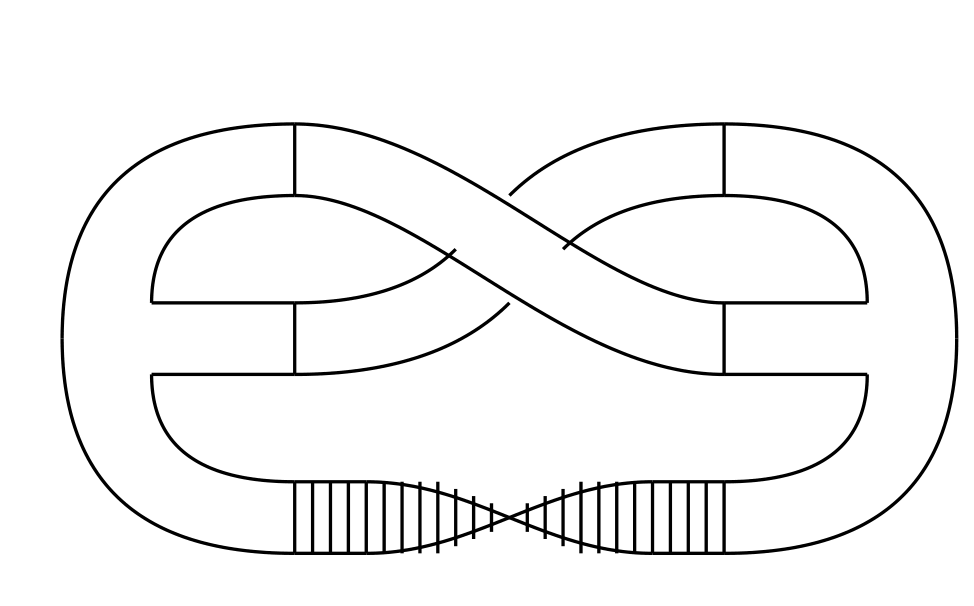
\includegraphics[width=4.12cm]{figures/fig-13.png}
  \caption{扭转胖图\figorig{56}{13}}
  \label{fig:13}
\end{figure}
 

现在，与 Hermitian 情形类似可以证明，$\log \widehat Z_N$ 的 $\frac{1}{N}$ 展开
（其中 $\widehat Z_N:=Z_N(\frac{2\hbar}{N}))$）由与前面相同的公式给出，只是求和改为遍历扭转胖图之集 $\widetilde G_c^{\rm tw}(\bold n)$：

\begin{theorem}\label{lnZ1}
$$
\log\widehat Z_N=
\sum_{\bold n}\prod_i (g_i\hbar^{\frac{i}{2}-1})^{n_i}
\sum_{\widetilde\Gamma\in \widetilde G_c^{\rm tw}(\bold n)}
\frac{N^{2-2{\rm g}(\widetilde\Gamma)}
}{|{\rm Aut}(\widetilde\Gamma)|}.
$$
\end{theorem}

这里，（可能不可定向的）曲面的亏格 ${\rm g}$ 对闭曲面用
${\rm g}:=1-\frac{\chi}{2}$ 定义，其中 $\chi$ 是欧拉示性数。于是 $\Bbb R\Bbb P^2$ 的亏格为 $\frac{1}{2}$，Klein 瓶的亏格为 $1$，如此等等。

特别地，我们有下述 't Hooft 定理的类比。

\begin{theorem} \label{tHooft1} (1) 存在极限 
$W_\infty:=\lim_{N\to \infty}\frac{\log\widehat Z_N}{N^2}$。该极限由下述公式给出：
$$
W_\infty=
\sum_{\bold n}\prod_i (g_i\hbar^{\frac{i}{2}-1})^{n_i}
\sum_{\widetilde\Gamma\in \widetilde G_c^{\rm tw}(\bold n)[0]}
\frac{1}{|{\rm Aut}(\widetilde\Gamma)|},
$$
其中 $\widetilde G_c^{\rm tw}(\bold n)[0]$ 表示\textbf{平面}连通扭转胖图之集，即亏格为零者。

(2) 此外，存在展开
$$
\frac{\log\widehat Z_N}{N^2}=\sum_{{\rm g}\in \frac{1}{2}\Bbb Z_{\ge 0}}a_{\rm g}N^{-2\rm g},
$$
其中
$$
a_{\rm g}=\sum_{\bold n}\prod_i (g_i\hbar^{\frac{i}{2}-1})^{n_i}
\sum_{\widetilde\Gamma\in \widetilde G_c^{\rm tw}(\bold n)[{\rm g}]}
\frac{1}{|{\rm Aut}(\widetilde\Gamma)|},
$$
而
$\widetilde G_c^{\rm tw}(\bold n)[{\rm g}]$ 表示亏格为 ${\rm g}$ 的连通扭转胖图之集。
\end{theorem}

\begin{exercise} 考虑在 $N$ 阶四元数 Hermitian 矩阵所成空间 ${\frak q}_N$ 上的矩阵积分。证明：此时结果与实情形相同，只是每个扭转胖图都带一个符号 $(-1)^\nu$，其中 $\nu$ 是边界分支的个数。换言之，$\log Z_N^{\rm quat}(\hbar)$ 等于把 $N$ 换成 $-N$ 后的 $\log Z_{2N}^{\rm real}(\hbar)$。

\textbf{提示：} 利用四元数酉群 $U(N,\Bbb H)$ 是 $Sp(2N)$ 的实形式，而 ${\frak q}_N$ 是表示 $\Lambda^2V$ 的实形式，其中 $V$ 是 $Sp(2N)$ 的标准（向量）表示。与实对称矩阵情形比较：那里相关的表示是 $O(N)$ 的 $S^2V$；而复数 Hermitian 矩阵情形则是 $GL(N)$ 的 $V\otimes V^*$。
\end{exercise} 

\subsection{由多边形粘合曲面的方式数与 Wigner 半圆律}

矩阵积分内容如此丰富，以至于最平凡的例子也会归结为一个不平凡的计数问题。具体地说，取复 Hermitian 矩阵上的矩阵积分 $Z_N$，令 $\hbar=1$ 并取
$S(A)=\frac{\Tr(A^2)}{2}-s\frac{\Tr(A^{2m})}{2m}$，其中 $s^2=0$
（即我们在环 $\Bbb C[s]/(s^2)$ 上工作）。则由定理 \ref{tHooft} 得到
$$
\int_{{\frak h}_N}\Tr(A^{2m})e^{-\frac{\Tr(A^2)}{2}}dA
=P_m(N),
$$
其中 $P_m(N)$ 是由公式
$$
P_m(N)=\sum_{{\rm g}\ge 0}\varepsilon_{\rm g}(m)N^{m+1-2\rm g},
$$ 
给出的多项式，而 $\varepsilon_{\rm g}(m)$ 是用一个有标号边的 $2m$ 边形粘合出亏格为 ${\rm g}$ 的曲面的方式数，即把各边配对、再把相配的边彼此保向地粘合起来的方式数。事实上，此时只有一个 $2m$ 价的胖花，它必须与自身粘合；因此直接应用我们的 Feynman 规则就归结为统计由多边形粘合出给定亏格曲面的方式数。

这个积分的值由下述不平凡的定理给出。

\begin{theorem} (Harer-Zagier, \cite{HZ} 1986) \label{howmany}
$$
P_m(x)=\frac{(2m)!}{2^mm!}\sum_{p=0}^m\begin{pmatrix}m\\ p\end{pmatrix}
2^p\frac{x(x-1) \ldots (x-p)}{(p+1)!}.
$$
\end{theorem}

该定理将在后面几个小节中证明。

考察 $P_m$ 的首项系数，即得

\begin{corollary}\label{Catalan}
用一个 $2m$ 边形粘合出球面的方式数，是 Catalan 数 $C_m=\frac{(2m)!}{m!(m+1)!}=\frac{1}{m+1}\binom{2m}{m}$。
\end{corollary}

推论 \ref{Catalan} 其实还有另一个（初等组合的）证明，如下所示。对 $2m$ 边形的边集上的每个匹配 $\sigma$，用直线段连接相配各边的中点（图 14）。从几何上看显然：若这些线段互不相交，则粘合给出球面。我们断言其逆亦真。事实上，设不然，即对循环排序的边 $a,b,c,d$，边 $a$ 与 $c$ 相连、$b$ 与 $d$ 相连。那么容易看出，把这两对边粘合起来会给出一个带孔的环面（$m=2$ 时则不带孔）。但带孔的（开）环面不能嵌入球面（例如它包含 $K_5$ 的一个拷贝），矛盾。

\begin{figure}[htbp]
  \centering
  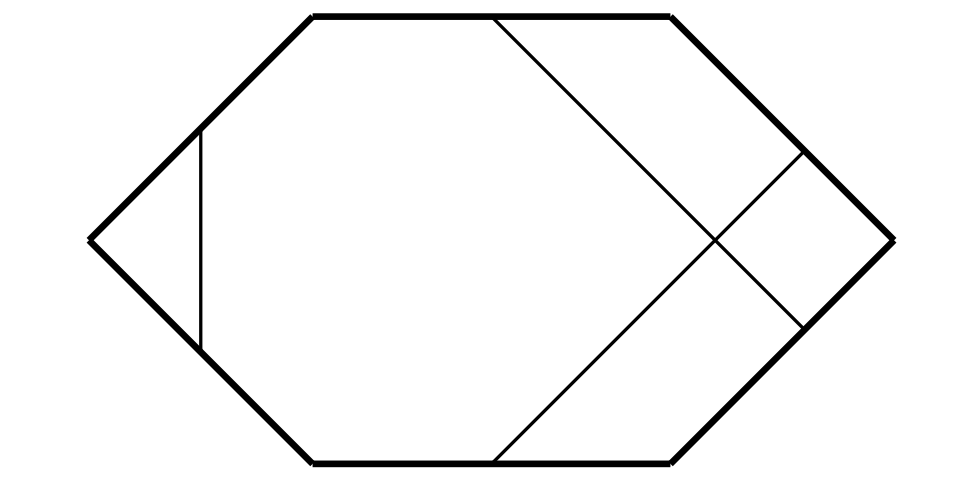
\includegraphics[width=4.04cm]{figures/fig-14.png}
  \caption{一个 $6$ 边形的边配对。\figorig{58}{14}}
  \label{fig:14}
\end{figure}

现在只剩下统计用互不相交的线段连接各边中点的方式数。假设我们画出这样一条线段，使其左侧有 $2k$ 条边、右侧有 $2l$ 条边（于是 $k+l=m-1$）。那么我们就面临把这两组各 $2k$ 与 $2l$ 条边用互不相交的线连接起来的问题。这表明粘合方式数 $D_m$ 满足递推
$$
D_m=\sum_{k+l=m-1}D_kD_l,\ D_0=1.
$$
换言之，生成函数
$$
h(x):=\sum_m D_mx^m=1+x+ \cdots
$$ 
满足方程 $h(x)-1=xh(x)^2$。由此得到
$$
h(x)=\frac{1-\sqrt{1-4x}}{2x},
$$ 
从而 $D_m=C_m$。证毕。

推论 \ref{Catalan} 可用来推出随机矩阵理论中的下述基本结果，它由 Wigner 于 1955 年发现。

\begin{theorem} (Wigner 半圆律)
设 $f$ 是 $\Bbb R$ 上在无穷远处至多多项式增长的连续函数。则
$$
\lim_{N\to \infty} \frac{1}{N}\int_{{\frak h}_N}{\rm }{\rm Tr} f(\tfrac{A}{\sqrt{N}})e^{-\frac{{\rm Tr}(A^2)}{2}}=
\frac{1}{2\pi}\int_{-2}^2f(x)\sqrt{4-x^2}dx.
$$
\end{theorem}

该定理之所以称为半圆律，是因为它说：按“高斯酉系综”（即密度为 $e^{-\frac{\Tr(A^2)}{2}}dA$）分布的大型随机 Hermitian 矩阵，其本征值密度的图形是半圆。特别地，我们看到对大的 $N$，$A$ 的几乎所有本征值都落在区间 $[-2\sqrt{N},2\sqrt{N}]$ 内，因此该极限与 $f$ 在 $[-2,2]$ 之外的值无关。
% [Tutor Note: 半圆律的矩方法：定理断言对任意多项式 f 有极限，而由 Catalan 数只验证了 f(x)=x^{2m} 的情形。半圆分布 \frac{1}{2\pi}\sqrt{4-x^2}dx 的 2m 阶矩正是 C_m（奇数阶矩为 0），例如 m=1 时 \frac{1}{2\pi}\int_{-2}^2 x^2\sqrt{4-x^2}dx=1。做替换 x=2\cos\theta 可化为 Beta 积分 \frac{2^{2m}}{\pi}\int_0^\pi\cos^{2m}\theta\sin^2\theta\,d\theta，其值为 \frac{(2m)!}{m!(m+1)!}。注意定理左边的归一化：f=1 时两边都等于 1，故文中 1/N 而非常见的 1/N^{m+1} 是正确的。]

\begin{proof} 
由 Weierstrass 关于闭区间上连续函数可被多项式一致逼近的定理，可以假定
$f$ 是多项式（习题：请论证这一步）。于是只需在
$f(x)=x^{2m}$ 时验证结论。此时由推论 \ref{Catalan}，左端等于 $C_m$。另一方面，初等计算给出
$$
\frac{1}{2\pi}\int_{-2}^2x^{2m}\sqrt{4-x^2}dx=C_m,
$$ 
由此即得定理。
\end{proof}

\subsection{Hermite 多项式}

下面给出的定理 \ref{howmany} 的证明\footnote{这个证明取自 D. Jackson 的讲义。}要用到 Hermite 多项式。因此先回顾它们的性质。

Hermite 多项式由公式
$$
H_n(x)=(-1)^ne^{x^2}\frac{d^n}{dx^n}e^{-x^2}.
$$
定义。于是 $H_n(x)$ 的首项为 $(2x)^n$。

我们在下述定理中汇集 $H_n(x)$ 的标准性质。
% [Tutor Note: 归一化约定在此务必留意：这里取权函数 e^{-x^2}（物理学家约定 H_n），因此 \frac{1}{\sqrt{\pi}}\int e^{-x^2}H_mH_n dx=2^nn!\delta_{mn}；若改用概率论约定 He_n（权 e^{-x^2/2}，即 ∫e^{-x^2/2}He_mHe_n=\sqrt{2\pi}n!\delta_{mn}），则定理 (iii)(iv)(v) 的所有常数都要改。另注意 (ii) 中 H_n(x)e^{-x^2/2} 是 L=-\frac12\partial^2+\frac12x^2 的本征函数，本征值 n+\frac12：权 e^{-x^2}=(e^{-x^2/2})^2 恰好来自把 L 的本征函数除以 e^{-x^2/2} 后去掉 Gaussian 因子，这一“权 = 波函数模方”的关系是正交性的来源。]

\begin{theorem} \label{Hermite}
(i) $H_n(x)$ 的指数生成函数为
$$
f(x,t)=\sum_{n\ge 0}H_n(x)\frac{t^n}{n!}
=e^{2xt-t^2}.
$$ 

(ii) $H_n(x)$ 满足微分方程
$f''-2xf'+2nf=0$。换言之，
$H_n(x)e^{-x^2/2}$ 是算子 $L=-\frac{1}{2}\partial^2+\frac{1}{2}x^2$（量子谐振子的哈密顿量）的本征函数，本征值为 $n+\frac{1}{2}$。

(iii) $H_n(x)$ 彼此正交：
$$
\frac{1}{\sqrt{\pi}}\int_{-\infty}^{\infty}e^{-x^2}H_m(x)H_n(x)dx=
2^nn!\delta_{mn}.
$$
此外，函数 $H_n(x)e^{-\frac{x^2}{2}}$ 构成 $L^2(\Bbb R)$ 的一组正交基。  

(iv) 有
$$
\frac{1}{\sqrt{\pi}}\int_{-\infty}^{\infty}e^{-x^2}x^{2m}H_{2k}(x)dx=
\frac{(2m)!}{(m-k)!}2^{2(k-m)}
$$
（若 $k>m$，答案为零）。

(v) 有
$$
\frac{H_r^2(x)}{2^rr!}=\sum_{k=0}^r\frac{r!}{2^kk!^2(r-k)!}H_{2k}(x).
$$
\end{theorem}
 
\begin{proof}（略证）
(i) 由算子 $\sum_{n\ge 0} (-1)^n\frac{t^n}{n!}\frac{d^n}{dx^n}$ 
把函数 $g(x)$ 映为 $g(x-t)$ 这一事实立得。

(ii) 由 (i) 以及函数 $f(x,t)$ 满足偏微分方程
$$
f_{xx}-2xf_x+2tf_t=0.
$$ 
即得。

(iii) 正交性可由 (i) 直接积分得到：
$$
\frac{1}{\sqrt{\pi}}\int_{\Bbb R}f(x,t)f(x,u)e^{-x^2}dx=\frac{1}{\sqrt{\pi}}\int_{\Bbb R}e^{2ut-(x-u-t)^2}dx=e^{2ut}.
$$ 
于是函数 $H_n(x)e^{-\frac{x^2}{2}}$ 在 $L^2(\Bbb R)$ 中构成正交系。

为说明这些函数是完备的，用 $E\subset L^2(\Bbb R)$ 记它们的张成 $\Bbb C[x]e^{-\frac{x^2}{2}}$ 的闭包。用 Taylor 多项式逼近函数 $e^{ipx}$，容易看出对任意 $p\in \Bbb R$ 都有 $e^{ipx-\frac{x^2}{2}}\in E$。
于是对任意紧支光滑函数 $\phi\in C_0^\infty(\Bbb R)$ 有
$$
\phi(x)e^{-\frac{x^2}{2}}=\int_{\Bbb R} \widehat \phi(p)e^{ipx-\frac{x^2}{2}}dp\in E.
$$
其中 $\widehat \phi$ 是 $\phi$ 的（适当归一化的）Fourier 变换。换言之，$C_0^\infty(\Bbb R)$ 在 $E$ 中稠密。
但 $C_0^\infty(\Bbb R)$ 显然在 $L^2(\Bbb R)$ 中稠密，故 $E=L^2(\Bbb R)$，如所断言。

(iv) 由 (i)，应计算
$\int_{\Bbb R}x^{2m}e^{2xt-t^2}e^{-x^2}dx$。
该积分等于
$$
\int_{\Bbb R}x^{2m}e^{-(x-t)^2}dx=\int_{\Bbb R}(y+t)^{2m}e^{-y^2}dy=
=\sqrt{\pi}
\sum_p \begin{pmatrix} 2m\\ 2p\end{pmatrix} \frac{(2m-2p)!}{2^{m-p}(m-p)!}t^{2p}.
$$
现在逐个提取系数即得结果。

(v) 由 (iii)，只需证明
$$
\frac{1}{\sqrt{\pi}}\int_{\Bbb R}H_r^2(x)H_{2k}(x)
e^{-x^2}dx=\frac{2^{r+k}r!^2(2k)!}{k!^2(r-k)!}
$$
为证此恒等式，把三个生成函数之积积分。由 (i) 有
$$
\frac{1}{\sqrt{\pi}}\int_{\Bbb R}f(x,t)f(x,u)f(x,v)e^{-x^2}dx=
$$
$$
\frac{1}{\sqrt{\pi}}\int_{\Bbb R}e^{2(ut+uv+tv)-(x-u-t-v)^2}dx
=e^{2(ut+tv+uv)}.
$$
提取 $t^ru^rv^{2k}$ 的系数即得结果。
\end{proof}

\subsection{定理 \ref{howmany} 的证明}
我们需要计算积分
$$
\int_{{\frak h}_N}\Tr(A^{2m})e^{-\frac{\Tr(A^2)}{2}}dA.
$$
为此注意被积函数在酉矩阵共轭下不变。因此该积分可以化为对 $A$ 的本征值 $\lambda_1, \ldots ,\lambda_N$ 的积分。

更确切地说，考虑谱映射 $\sigma: {\frak h}_N\to \Bbb R^N/S_N$。
众所周知（H. Weyl），直像
$\sigma_*dA$ 由公式
$\sigma_*dA=Ce^{-\sum_i\frac{\lambda_i^2}{2}}\prod_{i<j} (\lambda_i-\lambda_j)^2d\lambda$ 
给出，其中 $C>0$ 是一个与本文无关的归一化常数。于是有
$$
P_m(N)=\frac{NJ_m}{J_0},\ J_m:=\int_{\Bbb R^N}(\frac{1}{N}\sum_i\lambda_i^{2m})
e^{-\sum_i \frac{\lambda_i^2}{2}}\prod_{i<j} (\lambda_i-\lambda_j)^2d\lambda.
$$
为计算 $J_m$，我们将使用 Hermite 多项式。注意 $H_n(x)$ 是首项系数为 $2^n$ 的 $n$ 次多项式，故有
$$
\prod_{i<j}(\lambda_i-\lambda_j)= 2^{-\frac{N(N-1)}{2}}
\det (H_k(\lambda_\ell)),
$$ 
其中 $k$ 遍历集合
$0,1, \ldots ,N-1$，而 $\ell$ 遍历 $1,...,N$。于是得到
\begin{equation}
\begin{gathered}
J_m=2^{m+{N^2\over 2}}\int_{\Bbb R^N}\lambda_1^{2m}
e^{-\sum_i \lambda_i^2}\prod_{i<j} (\lambda_i-\lambda_j)^2d\lambda=\\ 
2^{m-{N(N-2)\over 2}}\int_{\Bbb R^N}\lambda_1^{2m}
e^{-\sum_i \lambda_i^2}\det(H_k(\lambda_j))^2d\lambda=\\ 
2^{m-{N(N-2)\over 2}}\sum_{\sigma,\tau\in S_N}(-1)^{\sigma}(-1)^{\tau}\int_{\Bbb R^N}\lambda_1^{2m}
e^{-\sum_i \lambda_i^2}
\prod_i H_{\sigma(i)}(\lambda_i)H_{\tau(i)}(\lambda_i)d\lambda.
\end{gathered}
\end{equation}
（这里 $(-1)^\sigma$ 表示 $\sigma$ 的符号）。

由于 Hermite 多项式正交，该和中只有满足 $\sigma(i)=\tau(i)$（$i=2, \ldots ,N$）的项非零。也就是说，非零项都满足 $\sigma=\tau$。于是有
\begin{equation}
\begin{aligned}
J_m=2^{m-{N(N-2)\over 2}}\sum_{\sigma\in S_N}
\int_{\Bbb R^N}\lambda_1^{2m}
e^{-\sum_i \lambda_i^2}
\prod_i H_{\sigma i}(\lambda_i)^2d\lambda=\\
2^{m-{N(N-2)\over 2}}(N-1)!\gamma_0 \ldots \gamma_{N-1}\sum_{j=0}^{N-1}
\frac{1}{\gamma_j}\int_{-\infty}^\infty x^{2m}H_j(x)^2e^{-x^2}dx,
\end{aligned}
\end{equation}
其中 $\gamma_i:=\int_{-\infty}^\infty H_i(x)^2e^{-x^2}dx$ 
是 Hermite 多项式的范数平方。对 $m=0$ 应用此式，并用 $J_0$ 除 $NJ_m$，得到
$$
P_m(N)=2^m\sum_{j=0}^{N-1}
\frac{1}{\gamma_j}\int_{-\infty}^\infty x^{2m}H_j(x)^2e^{-x^2}dx.
$$
利用定理 \ref{Hermite} 的 (iii) 与 (v) 可得
$\gamma_i=2^ii!\sqrt{\pi}$，从而
$$
P_m(N)=\frac{1}{\sqrt{\pi}}\int_{\Bbb R}\sum_{j=0}^{N-1}
\sum_{k=0}^j\frac{2^mx^{2m}H_{2k}(x)}{2^kk!^2(j-k)!}e^{-x^2}dx.
$$
现在利用定理 \ref{Hermite} 的 (iv)，得到
$$
P_m(N)=\frac{(2m)!}{2^m}\sum_{j=0}^{N-1}
\sum_{k=0}^j\frac{2^kj!}{(m-k)!k!^2(j-k)!}=
$$
$$
\frac{(2m)!}{2^mm!}\sum_{j=0}^{N-1}
\sum_{k=0}^j2^k\begin{pmatrix}m\\ k\end{pmatrix}
\begin{pmatrix}j\\ k\end{pmatrix}.
$$
对 $k$ 的求和可以表示为多项式的常数项：
$$
\sum_{k=0}^j2^k\begin{pmatrix}m\\ k\end{pmatrix}
\begin{pmatrix}j\\ k\end{pmatrix}=
C.T.((1+z)^m(1+2z^{-1})^j). 
$$
因此对 $j$ 求和（利用等比级数求和公式）给出
$$
P_m(N)=\frac{(2m)!}{2^mm!}
C.T.\left((1+z)^m\frac{(1+2z^{-1})^N-1}{2z^{-1}}\right)=
$$
$$
\frac{(2m)!}{2^mm!}\sum_{p=0}^m2^p
\begin{pmatrix}m\\ p\end{pmatrix}
\begin{pmatrix}N\\ p+1\end{pmatrix}.
$$
证毕。

\begin{exercise} 求用一个 $4{\rm g}$ 边形粘合出亏格 ${\rm g}\ge 1$ 的可定向曲面的方式数（粘合须保持定向），并证明你的答案。

\textbf{答案：} $\frac{(4{\rm g}-1)!!}{2{\rm g}+1}$。
\end{exercise} 

\begin{exercise} 考虑按高斯密度 $e^{-{\rm Tr}(A^2)}dA$ 分布的随机 Hermitian 矩阵 $A\in
{\frak h}_N$。证明：$A$ 最可能的本征值是第 $N$ 个 Hermite 多项式 $H_N$ 的根。

\textbf{提示。} 1) 写出密度在本征值上的极大值所满足的代数方程组。

2) 引入多项式 $P(z)=\prod_i(z-\lambda_i)$，其中 $\lambda_i$ 是最可能的本征值。令 $f=P'/P$。计算 $f'+f^2$（考察极点）。

3) 把所得的关于 $f$ 的 Riccati 方程化为关于 $P$ 的二阶线性微分方程。证明该方程就是 Hermite 方程，并由此推出 $P=\frac{H_N}{2^N}$。
\end{exercise} 

\bigskip
\noindent\rule{\textwidth}{0.6pt}
% [Tutor Note: 本章小结与自洽性核对——(1) 两个展开的幂次必须对得上：亏格展开定理中的 N^{2-2g} 与 \hbar^{b}（b=2g-2+\nu）在标度 \hbar\to\hbar/N 下由 \nu-b=2-2g 保证；(2) Harer–Zagier 公式的最高次项给出 Catalan 数推论 C_m=(2m)!/(m!(m+1)!)，即 \varepsilon_0(m) 的值；而 Wigner 半圆律的 2m 阶矩恰等于同一个 C_m，两条完全独立的推导在此会合，可作为公式正确性的强校验；(3) 半圆律的证明只逐项验证了多项式 f(x)=x^{2m}，由 Weierstrass 逼近与矩的唯一性（半圆分布的矩增长为 4^m，满足 Carleman 条件，故矩问题确定）即可推广到连续且多项式增长的 f；(4) 半圆律定理左边的归一化中 1/N 与 1/N^{m+1} 的差别容易出错：f=x^{2m} 时左端为 N^{-m-1}P_m(N)，其 N\to\infty 极限正是 \varepsilon_0(m)=C_m。]


%=====================================================================
% 5  曲线模空间的欧拉示性数
% 原文：Section 5. The Euler characteristic of the moduli space of curves
%       （arXiv:2409.03117v1, p. 63--74）
%=====================================================================
\section{曲线模空间的欧拉示性数}

\begin{keytakeaways}
\begin{itemize}
  \item \textbf{物理图像：}矩阵积分（特别是相关多项式的计算）不仅能给出多边形粘合数，还能进一步算出曲线模空间的轨形欧拉示性数；这正是 Harer 与 Zagier 在 1986 年完成的经典工作。
  \item \textbf{数学工具：}Wall 意义下的群欧拉示性数（有限群的取值为群阶的倒数）、轨形欧拉示性数、Quillen 的胞腔求和公式，以及 Mumford 关于 Teichmüller 空间组合模型的定理。
  \item \textbf{关键结论：}带一个标记点的曲线模空间，其轨形欧拉示性数等于 $-\frac{B_{2{\rm g}}}{2{\rm g}}$；不带标记点时则为 $\frac{B_{2{\rm g}}}{4{\rm g}({\rm g}-1)}$。
  \item \textbf{证明策略：}把填满弧系的计数化为“带限制的多边形粘合计数”，利用三种粘合计数（不加条件、满足条件 (A)、满足条件 (A)、(B)）之间的二项式卷积关系与生成函数，把所求之和化为 欧拉 Beta 积分，最后由 $\Gamma'/\Gamma$ 的 Stirling 渐近展开读出 Bernoulli 数。
  \item \textbf{易错点：}Quillen 公式按 $(-1)^{\dim\sigma}/|{\rm Stab}\,\sigma|$ 加权；Poincaré 对偶胞腔的维数为 $6{\rm g}-3-n$，故符号恰为 $(-1)^{n-1}$，这是本章最容易弄错符号之处。
\end{itemize}
\end{keytakeaways}

\bigskip
\noindent\rule{\textwidth}{0.6pt}
\bigskip

矩阵积分（特别是多项式 $P_m(x)$ 的计算）可用于计算曲线模空间的轨形欧拉示性数。这一工作由 Harer 与 Zagier 于 1986 年完成。本节我们回顾这一结果（有所省略）。

\subsection{群的欧拉示性数}

我们首先回顾代数拓扑中的一些基本概念。

设 $\Gamma$ 为离散群，$Y$ 为可缩的有限维 CW 复形，$\Gamma$ 在其上作胞腔作用。这指的是 $\Gamma$ 通过 $Y$ 的同胚作用，且把每个胞腔同胚地映到另一个胞腔。我们假定每个胞腔的稳定子都是有限群（亦即 $Y$ 是真 $\Gamma$-复形，proper $\Gamma$-complex）。

先设 $\Gamma$ 的作用是自由的（即胞腔的稳定子平凡）。这等价于说 $\Gamma$ 是无挠的（torsion free，即没有非平凡有限子群），因为有限群不可能无不动点地作用在可缩的有限维胞腔复形上（它的上同调维数是无限的）。

此时可以定义胞腔复形 $Y/\Gamma$（$\Gamma$ 的分类空间），并且对任意系数群 $A$ 有 $H^i(Y/\Gamma,A)=H^i(\Gamma,A)$。特别地，若 $Y/\Gamma$ 有限，则 $\Gamma$ 的上同调维数有限，且欧拉示性数 $\chi(\Gamma):=\sum_i (-1)^i\dim H^i(\Gamma,\Bbb Q)$ 等于 $\sum_i (-1)^in_i(Y/\Gamma)$，其中 $n_i(Y/\Gamma)$ 表示 $Y/\Gamma$ 中 $i$ 维胞腔的个数。

然而这一设定限制很强，因为它只允许上同调维数有限的群，特别地排除了所有非平凡的有限群。因此我们考虑更一般的设定：假定某个有限指数子群 $\Gamma'\subset \Gamma$（而非 $\Gamma$ 本身）满足上述条件。此时可以定义 $\Gamma$ 的 Wall 意义下的欧拉示性数，即有理数 $[\Gamma:\Gamma']^{-1}\chi(\Gamma')$。

容易验证，Wall 意义下的欧拉示性数可用下述 \emph{Quillen 公式} 计算：
$$
\chi(\Gamma)=\sum_{\sigma\in {\rm cells(Y)}/\Gamma}\frac{(-1)^{\dim
    \sigma}}{|{\rm Stab}\sigma|}.
$$
特别地，这个数与 $\Gamma'$ 的选取无关（这一点也容易直接验证）。

% [Tutor Note: 有限群情形的 $\chi(G)=|G|^{-1}$ 是理解“加权”的关键：取有限指数子群为平凡群，并把 $Y$ 取为单点、$G$ 平凡地作用其上，于是 Quillen 公式中只剩一个 0 维胞腔轨道，其稳定子为整个 $G$，贡献为 $1/|G|$。这正是轨形欧拉示性数按 $1/|{\rm Aut}(x)|$ 加权的来源，与通常的拓扑欧拉示性数（例如 $H/SL_2(\Bbb Z)\cong\Bbb C$ 的 $\chi=1$）截然不同，切勿混用。以上解释只是形式说明，此时作用并不自由。]
\begin{example} 若 $G$ 是有限群，则 $\chi(G)=|G|^{-1}$（取平凡群作为有限指数子群）。
\end{example}

\begin{example} $G=SL_2(\Bbb Z)$。该群含有一个指数为 12 的子群 $F$，它是由两个生成元生成的自由群（请自行验证！）。群 $F$ 的欧拉示性数为 $-1$，因为其分类空间 $Y/F$ 是“8”字形（亦即 $Y$ 是“8”字形的万有覆盖）。因此 $SL_2(\Bbb Z)$ 的欧拉示性数为 $-\frac{1}{12}$。
\end{example}

Wall 意义下的欧拉示性数在轨形框架下有几何解释。具体地说，设 $\Gamma$ 如上（即 $\chi(\Gamma)$ 是定义良好的有理数），$M$ 是可缩流形，$\Gamma$ 在其上自由且真不连续地作用。此时点的稳定子有限，故 $M/\Gamma$ 是轨形。特别地，这意味着每一点 $x\in M/\Gamma$ 都附有一个有限群 ${\rm Aut}(x)$，其阶 $\le [\Gamma:\Gamma']$。设 $X_m$ 为 $M/\Gamma$ 中由自同构群 ${\rm Aut}(x)$ 的阶等于 $m$ 的那些点 $x$ 组成的子集。常常出现 $X_m$ 具有有限胞腔复形的同伦型的情形。此时，$M/\Gamma$ 的\emph{轨形欧拉示性数}定义为
$$
\chi_{\rm orb}(M/\Gamma)=\sum_m\frac{\chi(X_m)}{m}.
$$

现在断言 $\chi_{\rm orb}(M/\Gamma)=\chi(\Gamma)$。事实上，考察投影 $M/\Gamma'\to M/\Gamma$，容易看出 $\chi_{\rm  orb}(M/\Gamma)=\frac{1}{[\Gamma:\Gamma']}\chi(M/\Gamma')$。但 $M/\Gamma'$ 是 $\Gamma'$ 的分类空间，故 $\chi(M/\Gamma')=\chi(\Gamma')$，由此即得断言。

\begin{example} 考虑群 $\Gamma=SL_2(\Bbb Z)$ 作用在上半平面 $H$ 上。此时 $H/\Gamma$ 是椭圆曲线的模空间。作为拓扑空间它是 $\Bbb C$，其中所有点的自同构群都是 $\Bbb Z/2$，例外的是点 $i$（自同构群为 $\Bbb Z/4$）以及 $\rho=\frac{-1+i\sqrt{3}}{2}$（自同构群为 $\Bbb Z/6$）。因此 $H/\Gamma$ 的轨形欧拉示性数为 $(-1)\frac{1}{2}+\frac{1}{4}+\frac{1}{6}=-\frac{1}{12}$。这并不奇怪，因为我们已经证明 $\chi_{\rm orb}(H/\Gamma)=\chi(\Gamma)$，而后者算得为 $-\frac{1}{12}$。
\end{example}

\subsection{映射类群}

设 ${\rm g}\ge 1$ 为整数，$\Sigma$ 是亏格为 ${\rm g}$ 的闭可定向曲面。取 $p\in \Sigma$，并令 $\Gamma_{\rm g}^1$ 为保持 $p$ 的 $\Sigma$ 的微分同胚的同痕类（isotopy class）构成的群。我们依照 Harer 与 Zagier 的文章 \cite{HZ}，不加证明地回顾关于该群的一些标准事实。

群 $\Gamma_{\rm g}^1$ 并非无挠，但它含有一个有限指数的无挠子群。具体而言，考虑由 $\Gamma_{\rm g}^1$ 在 $H_1(\Sigma,\Bbb Z/n\Bbb Z)$ 上的作用给出的同态 $\Gamma_{\rm g}^1\to {\rm Sp}(2{\rm g},\Bbb Z/n\Bbb Z)$。则当 $n$ 充分大时（事实上 $n\ge 3$），该映射的核 $K_n$ 是无挠的。

结果表明，存在一个可缩的有限维胞腔复形 $Y_{\rm g}$（将在下文构造），$\Gamma_{\rm g}^1$ 在其上作胞腔作用，且只有有限多个胞腔轨道。因此 $\Gamma_{\rm g}^1$ 的 Wall 意义下的欧拉示性数是定义良好的。

\subsection{Harer–Zagier 定理}

$\Gamma_{\rm g}^1$ 的欧拉示性数由下述定理给出。

\begin{theorem} \label{hz}（Harer–Zagier）有
$$
\chi(\Gamma_{\rm g}^1)=-\frac{B_{2{\rm g}}}{2{\rm g}},
$$
其中 $B_n$ 是 Bernoulli 数。
\end{theorem}

\begin{remark} 群 $\Gamma_{\rm g}^1$ 作用在 Teichmüller 空间 ${\mathcal T}_{\rm g}^1$ 上；按定义，后者是所有二元组 $((R,z),f)$ 构成的空间，其中 $(R,z)$ 是带标记点 $z$ 的复 Riemann 曲面，而 $f$ 是微分同胚 $R\to \Sigma$ 的同痕类，且把 $z$ 映到 $p$。可以证明 ${\mathcal T}_{\rm g}^1$ 是维数为 $6{\rm g}-4$ 的可缩流形，且 $\Gamma_{\rm g}^1$ 在 ${\mathcal T}_{\rm g}^1$ 上的作用是真不连续的。特别地，可以定义轨形 $M_{\rm g}^1={\mathcal T}_{\rm g}^1/\Gamma_{\rm g}^1$。该轨形参数化上述二元组 $(R,z)$，因此称为亏格为 ${\rm g}$、带一个标记点的 Riemann 曲面（即光滑复射影代数曲线）的模空间。于是定理 \ref{hz} 给出了亏格为 ${\rm g}$、带一个标记点的曲线模空间的轨形欧拉示性数。
\end{remark}

\begin{remark} 若 ${\rm g}>1$，可以定义上述对象不带标记点的类似物，即映射类群 $\Gamma_{\rm g}$、Teichmüller 空间 ${\mathcal T}_{\rm g}$ 与曲线模空间 $M_{\rm g}={\mathcal T}_g/\Gamma_g$（对 ${\rm g}=1$ 也可同样定义，但此时与带一个标记点的情形没有区别，因为平移群可以把 $\Sigma$ 上任意两点等同起来）。容易看出，当 ${\rm g}>1$ 时有正合列 $1\to \pi_1(\Sigma)\to \Gamma_{\rm g}^1\to \Gamma_{\rm g}\to 1$，由此可得 $\chi(\Gamma_{\rm g})=\chi(\Gamma_{\rm g}^1)/\chi(\Sigma)$。因此 Harer–Zagier 定理给出 $\chi(\Gamma_{\rm g})=\chi_{\rm orb}(M_{\rm g})=\frac{B_{2{\rm g}}}{4{\rm g}({\rm g}-1)}$。
\end{remark}

% [Tutor Note: 由正合列 $1\to\pi_1(\Sigma)\to\Gamma_{\rm g}^1\to\Gamma_{\rm g}\to 1$ 得到 $\chi(\Gamma_{\rm g})=\chi(\Gamma_{\rm g}^1)/\chi(\Sigma)$，用的是群扩张（纤维化）的欧拉示性数乘性 $\chi(\Gamma_{\rm g}^1)=\chi(\pi_1(\Sigma))\,\chi(\Gamma_{\rm g})$，其中 $\chi(\pi_1(\Sigma))=2-2{\rm g}$；不要与有限指数子群的公式 $\chi(\Gamma')=[\Gamma:\Gamma']\chi(\Gamma)$ 混淆（两者是不同层面的乘性）。代入 Harer–Zagier 公式：$-B_{2{\rm g}}/(2{\rm g})$ 除以 $2-2{\rm g}$ 恰得 $B_{2{\rm g}}/(4{\rm g}({\rm g}-1))$。注意 ${\rm g}=1$ 时 $\chi(\Sigma)=0$，公式分母 $4{\rm g}({\rm g}-1)$ 退化，正因如此第二个注只对 ${\rm g}>1$ 陈述。]

\subsection{复形 $Y_{\rm g}$ 的构造}

我们从复形 $Y_{\rm g}$ 的构造开始证明定理 \ref{hz}，仍依循 \cite{HZ}。先构造一个带 $\Gamma_{\rm g}^1$ 作用的单纯复形，再用它构造 $Y_{\rm g}$。

设 $(\alpha_1,...,\alpha_n)$ 是 $\Sigma$ 上的一族闭简单无向曲线，它们均以 $p$ 为起点与终点，且除 $p$ 外互不相交。若满足下列两个条件，则称这样的族为\emph{弧系}（arc system）：

(A) 任何一条曲线都不能收缩为一点；

(B) 任何一条曲线都不能收缩为另一条曲线。

定义单纯复形 $A$：其 $n-1$ 维单形是含 $n\ge 1$ 条弧的弧系的同痕类；对应于 $(\alpha_1,...\alpha_n)$ 的单形的边界，是对应于弧系 $(\alpha_1,...,\widehat\alpha_i,...,\alpha_n)$（即删去 $\alpha_i$）的各单形之并。

显然，群 $\Gamma_{\rm g}^1$ 在 $A$ 上作单纯作用。

\begin{example} 取 ${\rm g}=1$，即 $\Sigma=S^1\times S^1$。此时 $\Gamma_{\rm g}^1=SL_2(\Bbb Z)$。模去它的作用，只有三个弧系（图 15）。具体地说，把 $S^1$ 视为复平面中的单位圆并用参数表示弧，可把这三种弧系写成：
$$
B_0=\lbrace{(e^{i\theta},1)\rbrace}; B_1=
\lbrace{(e^{i\theta},1),(1,e^{i\theta})\rbrace};
B_2=\lbrace{(e^{i\theta},1),(1,e^{i\theta}),(e^{i\theta},e^{i\theta})\rbrace}
$$
由此容易求出单纯复形 $A$。具体地说，设 $T$ 是以 $t_0$ 为根、与三个顶点 $t_1,t_2,t_3$ 相连的树：每个 $t_i$ 又与两个顶点 $t_{i1},t_{i2}$ 相连，每个 $t_{ij}$ 再与 $t_{ij1},t_{ij2}$ 相连，如此继续（图 16）。在 $T$ 的每个顶点处放一个三角形，使其边横截于由该顶点出发的三条棱，再把这些三角形沿它们的边粘合起来。这样得到的复形就是 $A$，见图 17（请自行验证！）。$SL_2(\Bbb Z)$（更确切地说 $PSL_2(\Bbb Z)$）在该复形上的作用容易描述。具体地说，回忆 $PSL_2(\Bbb Z)$ 由 $S,U$ 生成，定义关系为 $S^2=U^3=1$。$S,U$ 在 $T$ 上的作用如下：$S$ 是关于以 $t_0$ 为中心的三角形 $\Delta_0$ 的一条边的带翻转的反射（图 18），$U$ 是绕 $t_0$ 的 $2\pi/3$ 旋转。
\end{example}

\begin{figure}[htbp]
  \centering
  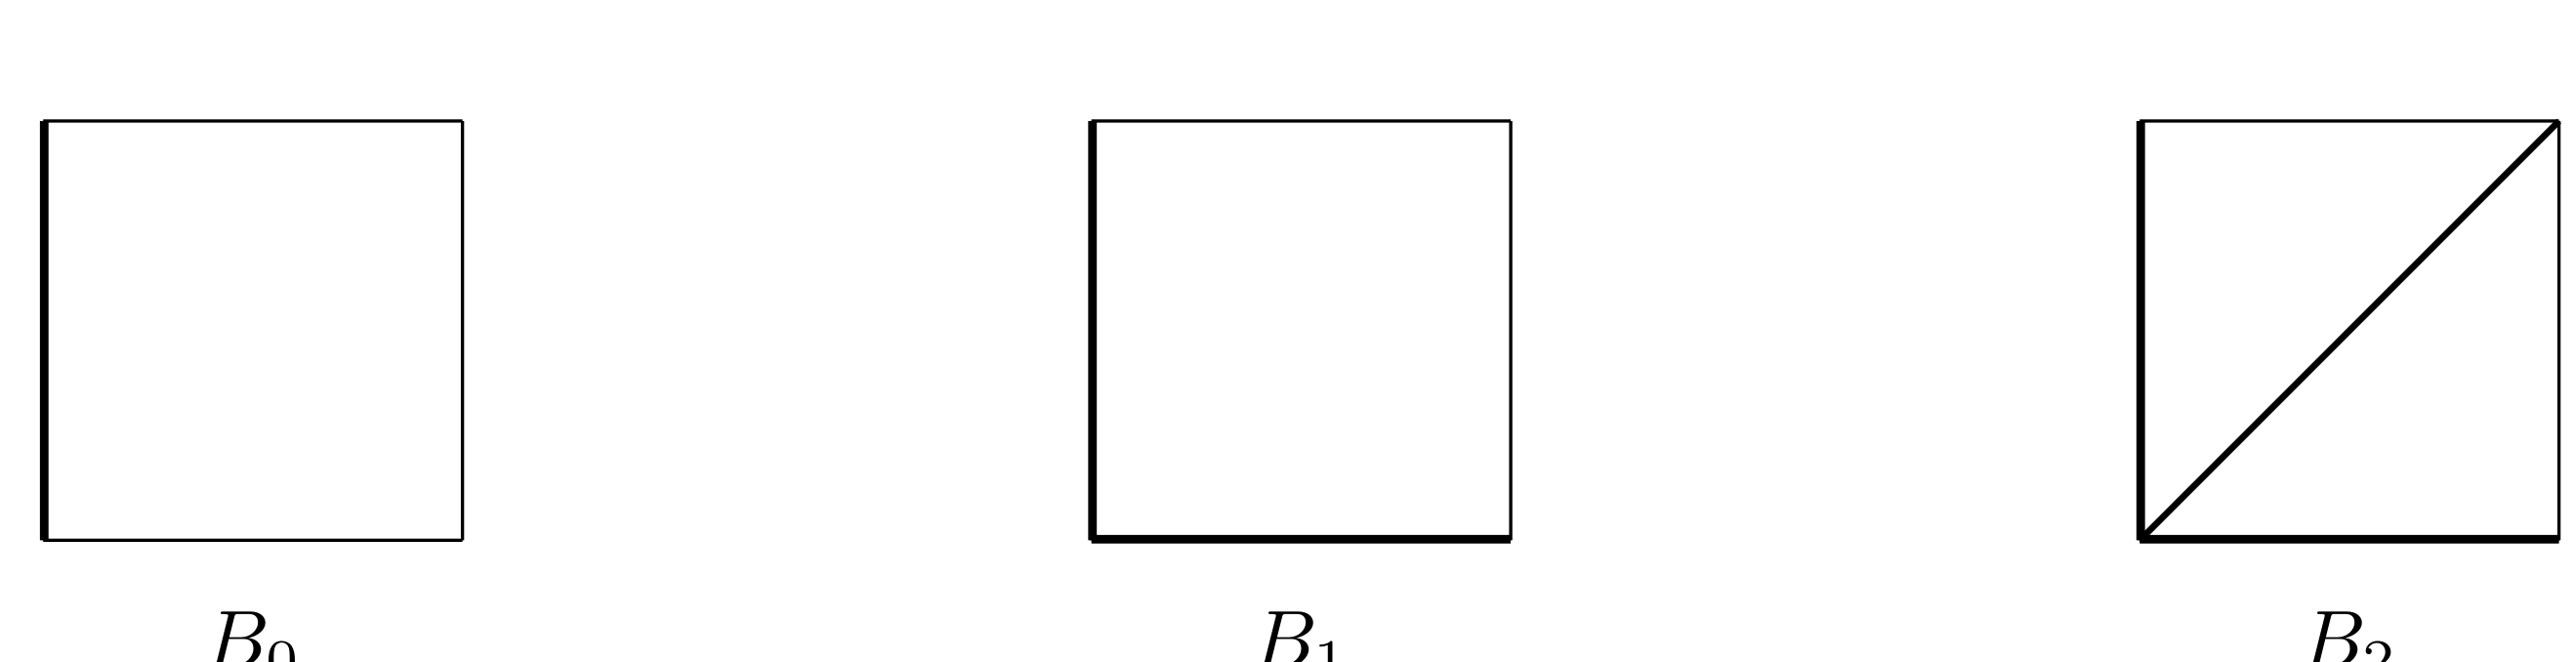
\includegraphics[width=11.16cm]{figures/fig-15.png}
  \caption{三个弧系。\figorig{67}{15}}
  \label{fig:15}
\end{figure}



\begin{figure}[htbp]
  \centering
  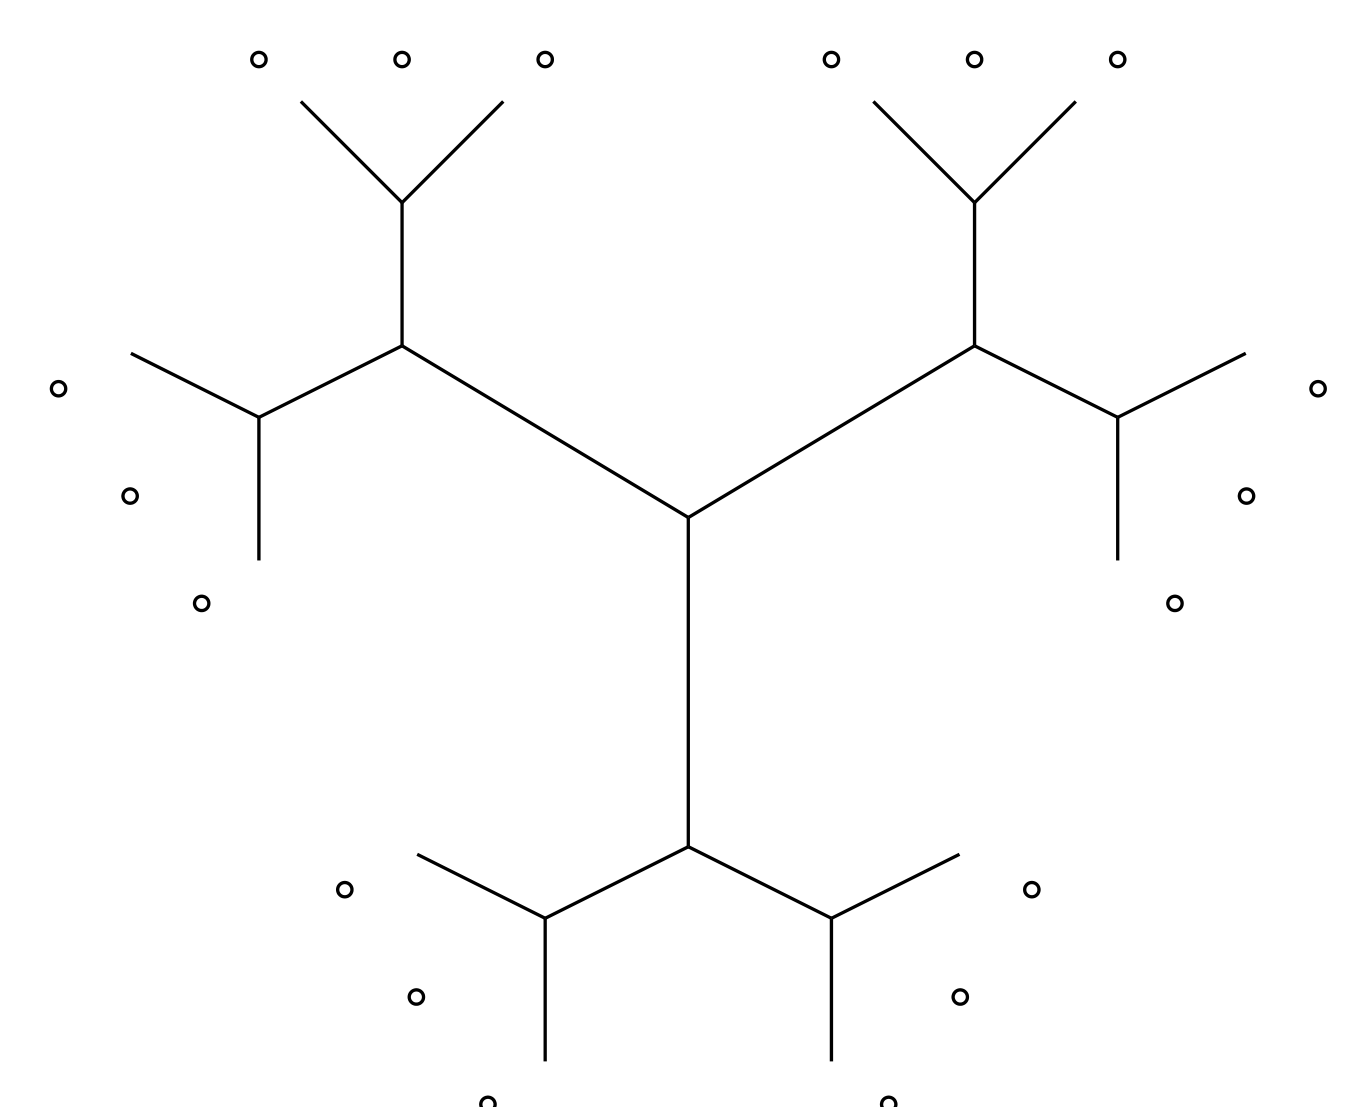
\includegraphics[width=5.71cm]{figures/fig-16.png}
  \caption{树 $T$\figorig{67}{16}}
  \label{fig:16}
\end{figure}


\begin{figure}[htbp]
  \centering
  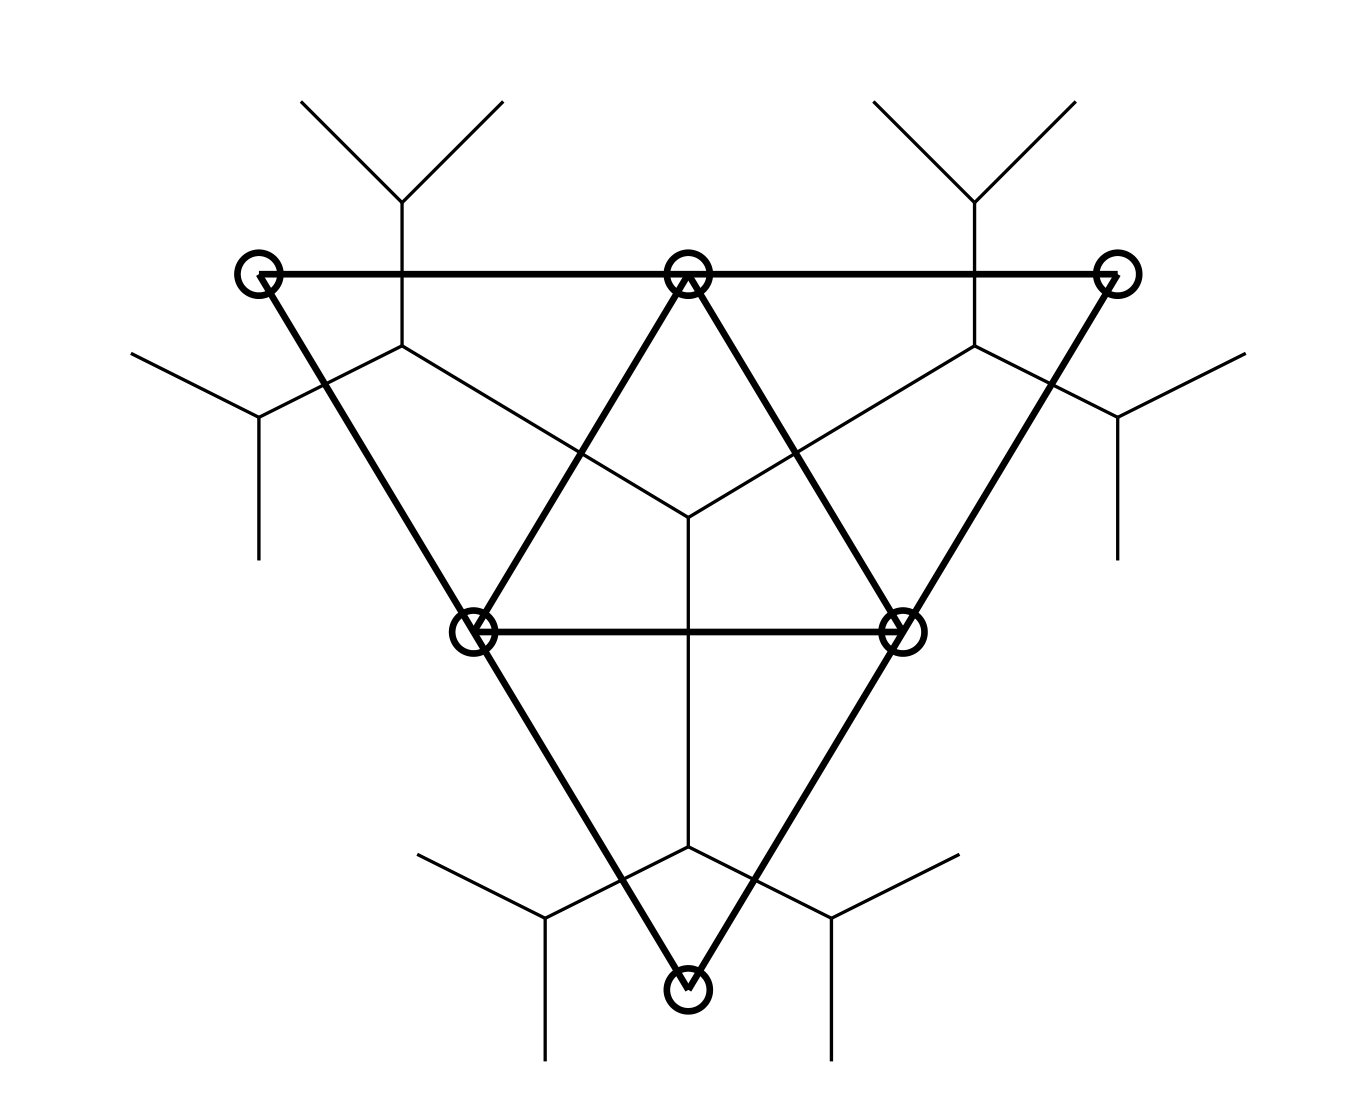
\includegraphics[width=5.71cm]{figures/fig-17.png}
  \caption{复形 A\figorig{68}{17}}
  \label{fig:17}
\end{figure}


\begin{figure}[htbp]
  \centering
  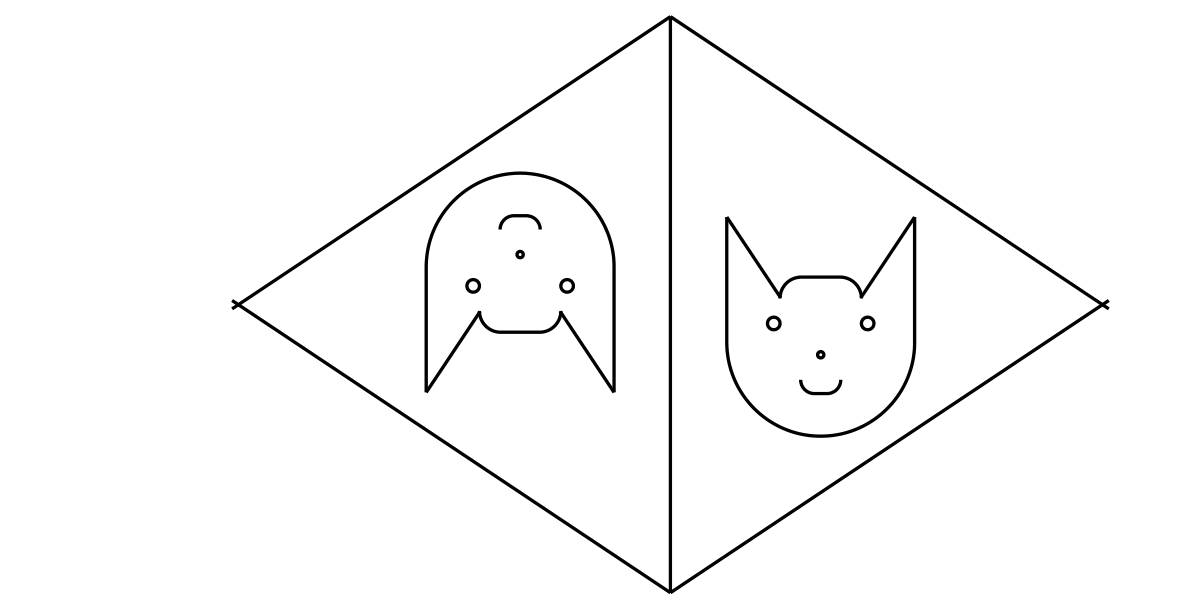
\includegraphics[width=5.03cm]{figures/fig-18.png}
  \caption{带翻转的反射。\figorig{68}{18}}
  \label{fig:18}
\end{figure}


这一例子表明，$\Gamma_{\rm g}^1$ 在 $A$ 上的作用并非真不连续，因为某些单形具有无限稳定子（在上例中就是 0 维单形）。因此我们希望丢掉这些“坏”单形。为此，若弧系 $(\alpha_1,..,\alpha_n)$ 把 $\Sigma$ 割成若干同胚于开圆盘的区域之并，则称它\emph{填满} $\Sigma$。令 $A_\infty$ 为 $A$ 中对应于不能填满 $\Sigma$ 的弧系的单形之并。这是闭子集，因为“不能填满 $\Sigma$”这一性质在取弧子系统时显然保持。因此 $A\setminus A_\infty$ 是 $A$ 的开子集。在上述例子中，它就是去掉 $0$ 维单形后的复形 $A$。

下述定理表明，$A\setminus A_\infty$ 实际上是带 $\Gamma_{\rm g}^1$ 作用的 Teichmüller 空间 ${\mathcal T}_{\rm g}^1$ 的一个组合模型。

\begin{theorem} \label{mum}（Mumford）
(a) $\Gamma_{\rm g}^1$ 在 $A\setminus A_\infty$ 上的作用是真不连续的。

(b) $A\setminus A_\infty$ 在拓扑上是一个流形，它与 Teichmüller 空间 ${\mathcal T}_{\rm g}^1$ 有 $\Gamma_{\rm g}^1$-等变的同胚；特别地，它是可缩的。
\end{theorem}

\begin{remark} 定理 \ref{mum} 揭示了条件 (A) 与 (B) 的意义。事实上，若去掉其中任何一个条件，就可以考虑 $n$ 任意大的弧系 $(\alpha_1,...,\alpha_n)$；而在条件 (A)、(B) 之下，由定理 \ref{mum} 可见 $n$ 的最大值为 $6{\rm g}-3$。
\end{remark}

\begin{remark} 当 ${\rm g}=1$ 时，由 $A$ 的显式描述即可看出定理 \ref{mum} 成立（请自行说服自己！）。
\end{remark}

定理 \ref{mum} 相当深刻，其证明超出本书范围，我们不予给出。我们只用它来定义 $A\setminus A_\infty$ 的“Poincaré 对偶”CW 复形 $Y_{\rm g}$。具体地说，对每个填满的弧系 $(\alpha_1,...,\alpha_n)$ 指定一个 $6{\rm g}-3-n$ 维胞腔，而边界关系与先前的相反。该 CW 复形的存在性来自 $A\setminus A_\infty$ 是流形这一事实。例如在 ${\rm g}=1$ 的情形，复形 $Y_{\rm g}$ 就是树 $T$。

现在，复形 $Y_{\rm g}$ 是可缩的（因为 $A\setminus A_\infty$ 也可缩），并且容许 $\Gamma_{\rm g}^1$ 的胞腔作用，胞腔轨道有限、稳定子有限。这意味着 $\Gamma_{\rm g}^1$ 的欧拉示性数由 Quillen 公式给出。
$$
\chi(\Gamma_{\rm g}^1)=\sum_{\sigma\in {\rm
    cells}(Y_{\rm g})/\Gamma_{\rm g}^1}
(-1)^{\dim\sigma}\frac{1}{|{\rm Stab\sigma}|}.
$$

% [Tutor Note: 这里最容易错的是维数与符号的对应。$A\setminus A_\infty$ 是 $6{\rm g}-4$ 维流形（即 Teichmüller 空间的实维数），填满弧系 $(\alpha_1,...,\alpha_n)$ 对应 $A$ 中的 $(n-1)$ 维单形；Poincaré 对偶把 $k$ 维胞腔换成 $(6{\rm g}-4-k)$ 维胞腔，故 $Y_{\rm g}$ 中对应胞腔的维数为 $6{\rm g}-3-n$。于是 $(-1)^{\dim\sigma}=(-1)^{6{\rm g}-3-n}=(-1)^{n-1}$（$6{\rm g}-3$ 为奇数），这正是下一节命题中符号 $(-1)^{n-1}$ 的来源；若写成 $(-1)^n$ 或 $(-1)^{n+1}$，最终会与 Harer–Zagier 公式差一个整体符号。]

\begin{example} 在 ${\rm g}=1$ 的情形，$T$ 有一个 $0$ 维胞腔轨道和一个 $1$ 维胞腔轨道。在 $SL_2(\Bbb Z)$ 中，0 维胞腔的稳定子是 $\Bbb Z/6$，1 维胞腔的稳定子是 $\Bbb Z/4$。因此 $\chi(SL_2(\Bbb Z))=\frac{1}{6}-\frac{1}{4}=-\frac{1}{12}$，这与前面用其他方法算得的结果一致。
\end{example}

\subsection{$Y_{\rm g}/\Gamma_{\rm g}^1$ 中胞腔的枚举}

现在只剩数清 $Y_{\rm g}/\Gamma_{\rm g}^1$ 中的胞腔，即枚举填满 $\Sigma$ 的弧系（并计入符号与稳定子）。为此注意，按“填满”的定义，任何填满的弧系 $S$ 都给出 $\Sigma$ 的一个胞腔分解。于是令 $S^*$ 为该胞腔分解的 Poincaré 对偶。由于 $S$ 有唯一的零维胞腔，$S^*$ 有唯一的二维胞腔。设 $n$ 为 $S$（或 $S^*$）中一维胞腔的个数。则 $(\Sigma, S^*)$ 可由一个 $2n$ 边形（即唯一的二维胞腔）按保持定向的边的配对粘合得到。（注意 $S$ 可由 $(S^*)^*$ 重构。）

这就把枚举填满弧系的问题与计数此类粘合的问题联系起来，而后者已用矩阵积分解决。具体地说，填满弧系的枚举问题实质上已经解决，只余一个复杂之处：由于弧系上的条件 (A) 与 (B)，我们得到的粘合并非任意粘合，而是还须满足某些条件的粘合。确切地说，有

\begin{lemma}
设 $(\alpha_1,...,\alpha_n)$ 是一族曲线，满足填满弧系的诸公理，但条件 (A) 与 (B) 可以例外。则

(i) $(\alpha_1,...,\alpha_n)$ 满足条件 (A) 当且仅当相应粘合中没有一条边粘到相邻的边。

(ii) $(\alpha_1,...,\alpha_n)$ 满足条件 (B) 当且仅当没有两条相邻的边按相反顺序粘到另一对相邻的边。
\end{lemma}

\begin{figure}[htbp]
  \centering
  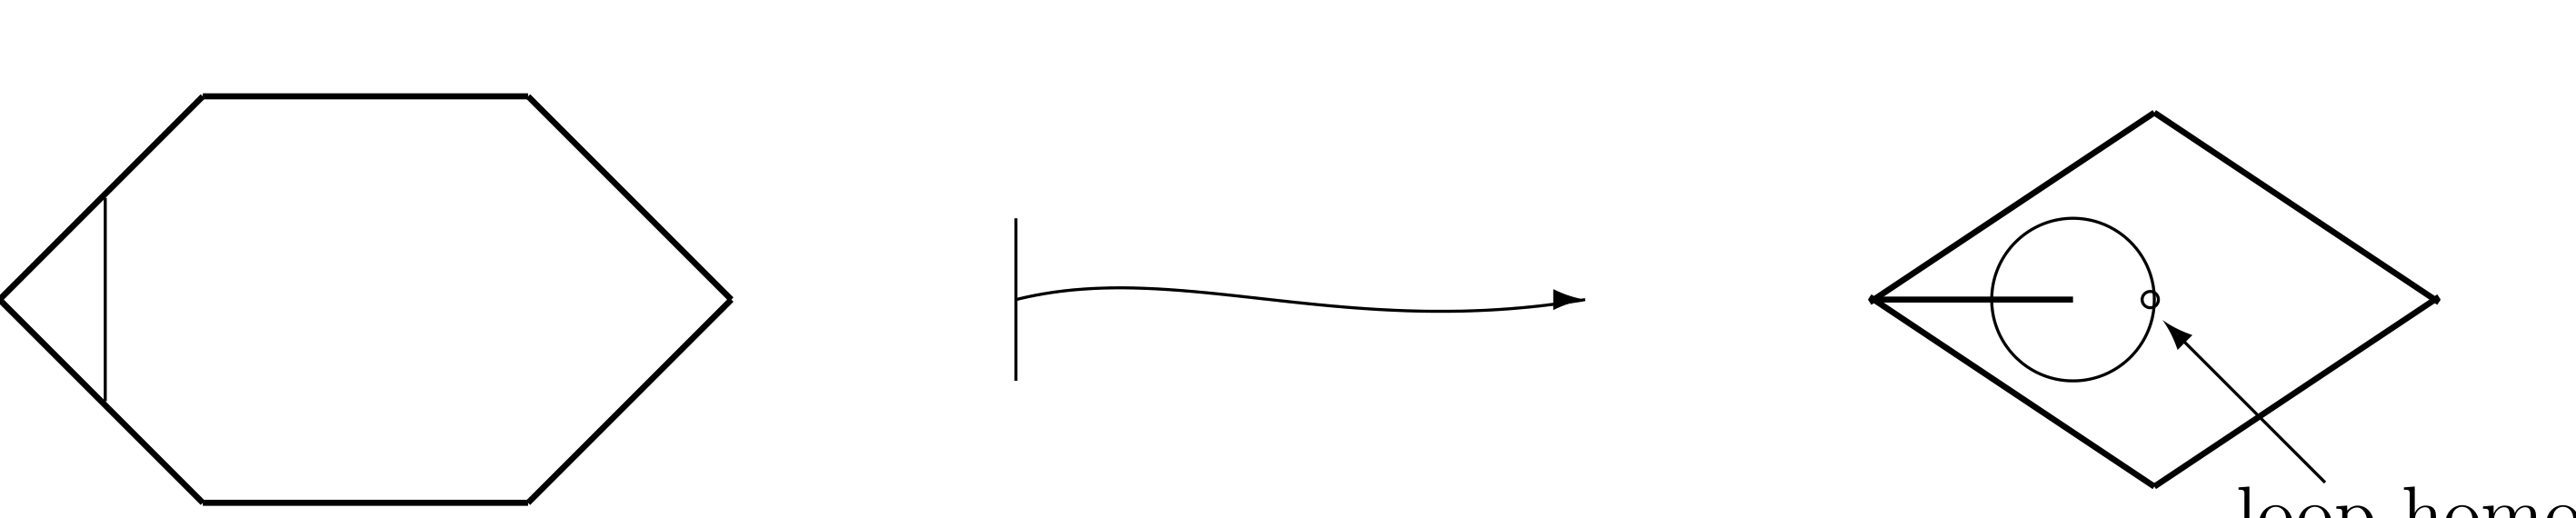
\includegraphics[width=12.0cm]{figures/fig-19.png}
  \caption{（原文无图题）\figorig{70}{19}}
  \label{fig:19}
\end{figure}


\begin{figure}[htbp]
  \centering
  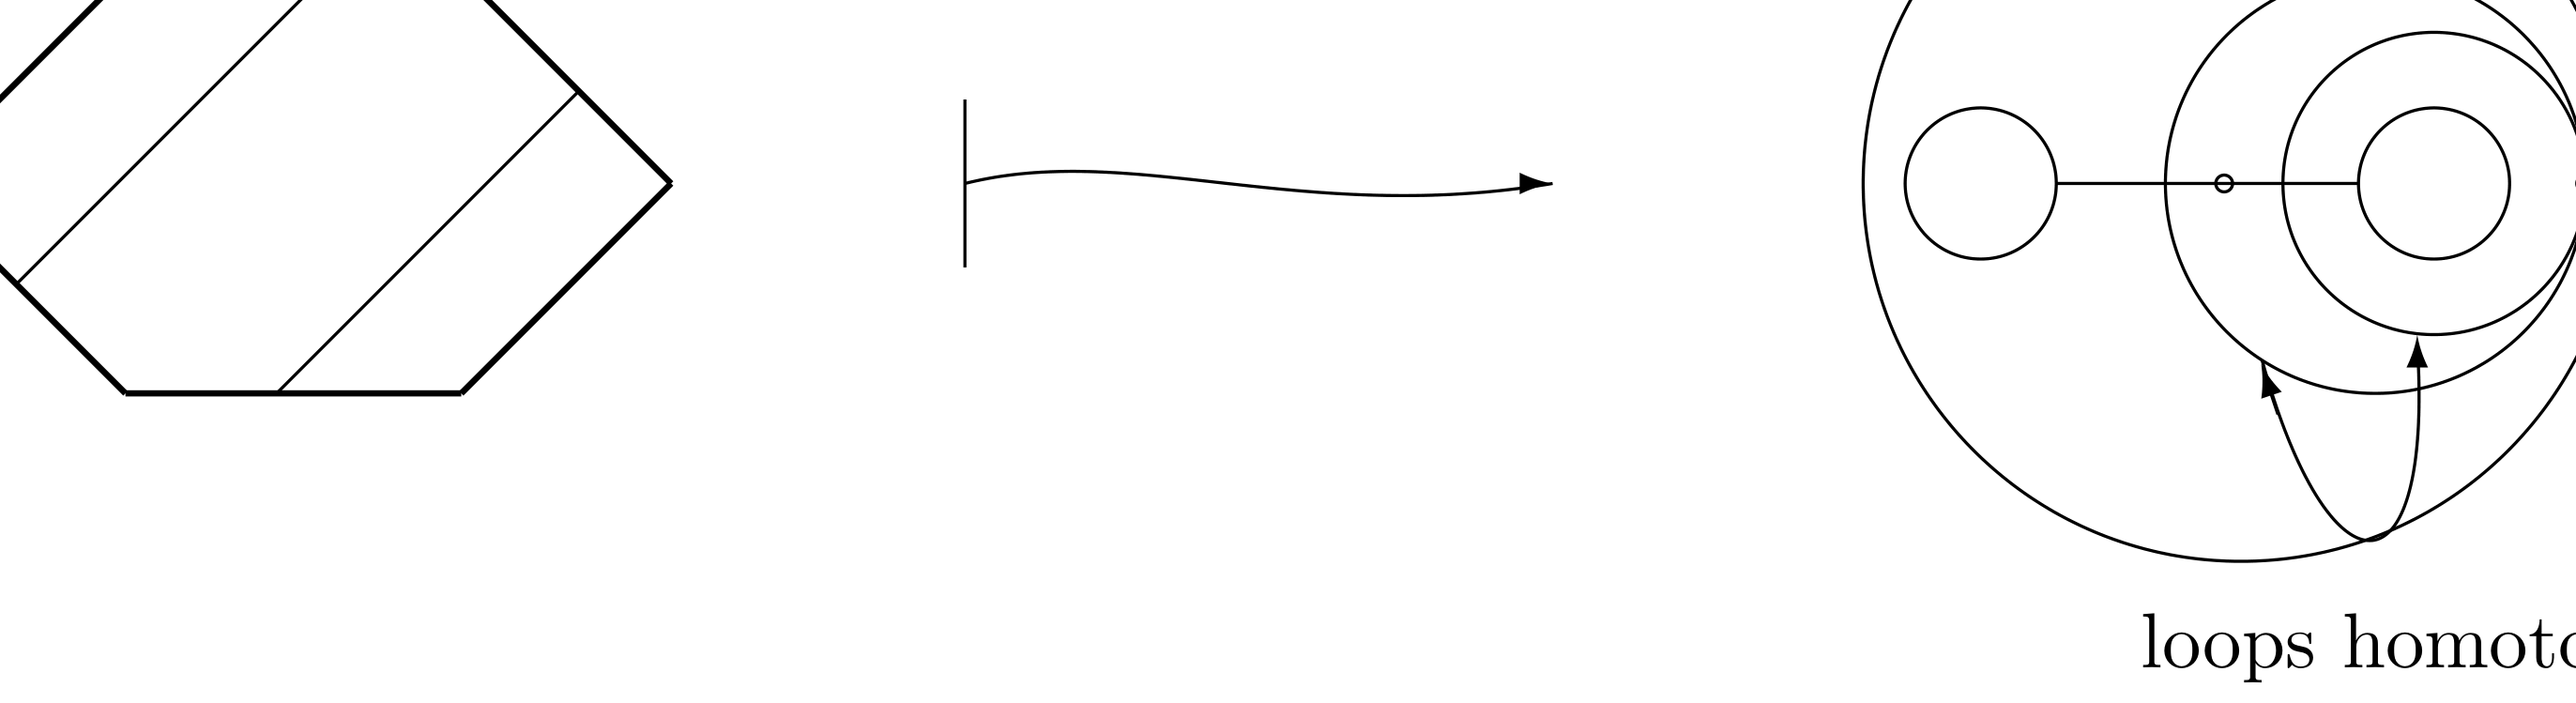
\includegraphics[width=11.62cm]{figures/fig-20.png}
  \caption{（原文无图题）\figorig{70}{20}}
  \label{fig:20}
\end{figure}


该引理在几何上显而易见，其证明只需画图（(i) 见图 19，(ii) 见图 20）。受该引理启发，我们也把 (i) 与 (ii) 中关于粘合的条件称为条件 (A) 与 (B)。

用 $\varepsilon_{\rm g}(n),\mu_{\rm g}(n),\lambda_{\rm g}(n)$ 分别表示把一个（带标号的）$2n$ 边形粘合成亏格为 ${\rm g}$ 的曲面的粘合数：分别不加任何条件、满足条件 (A)、满足条件 (A),(B)（因此 $\varepsilon_{\rm g}(n)$ 就是我们此前研究过的量）。

\begin{proposition} 有\footnote{注意对几乎所有的 $n$ 都有 $\lambda_{\rm g}(n)=0$，因此该和为有限和。}
$$
\chi(\Gamma_{\rm g}^1)=\sum_n (-1)^{n-1}\frac{\lambda_{\rm g}(n)}{2n}.
$$
\end{proposition}

\begin{proof}
每个填满弧系 $\sigma$ 来自 $2n/|{\rm Stab(\sigma)}|$ 个粘合（因为对所得的带弧系曲面而言，多边形的标号无关紧要）。于是结论由 Quillen 公式得出。
\end{proof}

\subsection{$\sum_n (-1)^{n-1}\frac{\lambda_{\rm g}(n)}{2n}$ 的计算}

现在只剩计算右端的和。为此需要把 $\lambda_{\rm g}(n)$ 与已经算出的 $\varepsilon_{\rm g}(n)$ 联系起来。这由下述引理完成。

\begin{lemma}\label{rel}
(i) 有
$$
\varepsilon_{\rm g}(n)=\sum_i \begin{pmatrix}2n\\ i\end{pmatrix}
\mu_{\rm g}(n-i).
$$
(ii) 有
$$
\mu_{\rm g}(n)=\sum_i \begin{pmatrix}n\\ i\end{pmatrix}
\lambda_{\rm g}(n-i).
$$
\end{lemma}

\begin{proof}(i) 设 $\sigma$ 是顶点带标号的 $2n$ 边形 $\Delta$ 的边的配对。若存在一对相邻的边被配对，就可以把它们互相粘合起来，得到 $2n-2$ 边形。如此尽可能地进行下去，最终得到 $2n-2i$ 边形 $\Delta_\sigma$ 及其边的一个满足条件 (A) 的配对 $\sigma'$。注意 $\Delta_\sigma$ 与 $\sigma'$ 不依赖于相邻边粘合的先后次序，并且 $\Delta_\sigma$ 有一个由“旧”标号递增顺序给出的标准标号 $1,...,2n-2i$。现在断言每个 $(\Delta_\sigma,\sigma')$ 恰好以 $\begin{pmatrix}2n\\ i\end{pmatrix}$ 种方式得到；这就给出所需结论。

事实上，考察 $\Delta$ 中最终落入 $\Delta_\sigma$ 内部的顶点。它们被映为内部的 $i$ 个点（每粘合一对边就产生一个新点）。称这些点为 $w_1,...,w_i$，并令 $\nu_j$ 为映到 $w_j$ 的 $\Delta$ 的顶点的最小标号（这里顶点标号使第 $k$ 条边连接顶点 $k$ 与顶点 $k+1$）。则 $\nu_1,...,\nu_i$ 是 $\lbrace{1,...,2n\rbrace}$ 的一个子集。在给定 $(\Delta_\sigma,\sigma')$ 时，这个子集完全决定了配对 $\sigma$：具体地说，应选出一个 $\nu_j$，使得对任意 $k$ 都有 $\nu_{j}+1\ne \nu_k$，然后把与 $\nu_j$ 相邻的两条边粘合；再把其余顶点按“旧”标号的递增顺序重新标为 $1,...,2n-2$，然后重复上述步骤，如此继续。由此也可看出，任何这样的 $\nu_j$ 集合都可能出现。这就证明了 (i)。

(ii) 设 $\sigma$ 是 $\Delta$（其边带标号）的配对，满足条件 (A)，但不必满足 (B)。若 $a_1,a_2$ 是相邻的边，且按相反顺序粘到相邻的边 $b_2,b_1$ 上，则可以把 $a_1,a_2$ 合并成一条边 $a$，把 $b_2,b_1$ 合并成 $b$，得到一个带配对的 $2n-2$ 边形。如此尽可能地进行下去，最终得到带新配对 $\sigma'$ 的 $2n-2i$ 边形 $\Delta_\sigma$，且该配对满足条件 (A) 与 (B)。在 $\Delta_\sigma$ 中，每一对（第 $j$ 对）边都是由 $\Delta$ 中的 $m_j+1$ 对边得到的。于是 $\sum_{j=1}^{n-i}m_j=i$。此外，对任意 $(\Delta_\sigma,\sigma')$，数集 $m_1,...,m_{n-i}$ 唯一确定了 $(\Delta,\sigma)$，只差确定构成 $\Delta_\sigma$ 第一条边的 $m_1+1$ 条边中哪一条应标为 1。因此每个 $(\Delta_\sigma,\sigma')$ 出现的次数由下述公式给出：
$$
\sum_{m_1,...,m_{n-i}:\sum_{j=1}^{n-i} m_j=i}(m_1+1).
$$
容易证明（请自行验证！）这个数等于 $\begin{pmatrix}n\\ i\end{pmatrix}$。这就证明了 (ii)。
\end{proof}

% [Tutor Note: 证明 (ii) 中“容易证明（请自行验证！）”掩盖了一个标准的组合恒等式：把 $i$ 分成 $n-i$ 个非负整数 $m_1,...,m_{n-i}$ 的有序分拆，求和 $\sum (m_1+1)$。其中分拆的个数为 $\binom{n-1}{i}$，而由对称性 $\sum m_1=\frac{i}{n-i}\binom{n-1}{i}=\binom{n-1}{i-1}$（各部分的地位对称，总和为 $i\binom{n-1}{i}$ 均摊到 $n-i$ 个位置），两者相加恰为 $\binom{n-1}{i}+\binom{n-1}{i-1}=\binom{n}{i}$。这就是 (ii) 中被略去的“一步”。]

定理 \ref{hz} 证明的完成现在依赖于下述计算引理。

\begin{lemma}\label{tech}
设 $\varepsilon(n),\mu(n),\lambda(n)$（$n\ge 0$）是满足方程
$$
\varepsilon(n)=\sum_i \begin{pmatrix}2n\\ i\end{pmatrix}
\mu(n-i);
$$
$$
\mu(n)=\sum_i \begin{pmatrix}n\\ i\end{pmatrix}
\lambda(n-i).
$$
的数列。并设 $\varepsilon(n)=\binom{2n}{
  n}f(n)$，其中 $f$ 是满足 $f(0)=0$ 的多项式。则 $\lambda(0)=0$，$\lambda(n)$ 只有有限多个非零值，且
$$
\sum_{n\ge 1} (-1)^{n-1}\frac{\lambda(n)}{2n}=f'(0).
$$
\end{lemma}

\begin{proof}
先考虑由引理中方程联系起来的任意数列 $\varepsilon(n)$、$\mu(n)$、$\lambda(n)$。设 $E(z)$、$M(z)$、$L(z)$ 为它们的生成函数（即 $E(z)=\sum_{n\ge 0}\varepsilon(n)z^n$ 等等）。我们断言
$$
E(z)=\frac{1+\sqrt{1-4z}}{2(1-4z)}L\left(\frac{1-\sqrt{1-4z}}{2\sqrt{1-4z}}\right).
$$
为看出这一点，只需考虑某个 $k$ 对应的情形 $\lambda_i=\delta_{ki}$。此时
$$
E(z)=\sum_{i,n}\begin{pmatrix} 2n\\ i\end{pmatrix}
\begin{pmatrix} n-i\\ k\end{pmatrix}z^n=
\sum_{p,q\ge 0}\begin{pmatrix} 2p+2q\\ p\end{pmatrix}
\begin{pmatrix} q\\ k\end{pmatrix}z^{p+q}.
$$
但函数
$$
F_r(z):=\sum_{p\ge 0}\begin{pmatrix} 2p+r\\ p\end{pmatrix}z^p
$$
等于
$$
F_r(z)=
\frac{1}{\sqrt{1-4z}}\biggl(\frac{1-\sqrt{1-4z}}{2z}\biggr)^r,
$$
这由递推
$$
F_r=z^{-1}(F_{r-1}-F_{r-2}),
$$
（$r\ge 2$）用归纳法容易看出。把它代入 $E(z)$ 的公式，经过平凡的化简即得
$$
E(z)=\frac{1+\sqrt{1-4z}}{2(1-4z)}\left(\frac{1-\sqrt{1-4z}}{2\sqrt{1-4z}}\right)^k,
$$
正是所要求的。

现在假设 $\varepsilon(n)$ 满足多项式性条件。这意味着 $E(z)=P(z\partial)|_{z=0}\frac{1}{\sqrt{1-4z}}$，其中 $P$ 是常数项为零的多项式。为证明我们的断言，只需考虑情形 $P(z)=(1+a)^z-1$，其中 $a$ 是形式参数（于是 $P'(0)=\log(1+a)$）；事实上该形式级数的系数是 $\binom{z}{j}$（$j\ge 1$），它们在常数项为零的 $z$ 的多项式空间中构成一组基。此时得到
$$
E(z)=\frac{1}{\sqrt{1-4(1+a)z}}-\frac{1}{\sqrt{1-4z}}.
$$
因此
$$
L(u)=\frac{1}{1+u}\left(\frac{1}{\sqrt{1-4au(1+u)}}-1\right).
$$
从而
$$
\sum_k (-1)^{k-1}\frac{\lambda_k}{2k}=\frac{1}{2}\int_{-1}^0 L(u)\frac{du}{u}=
\frac{1}{2}\sum_{p\ge 1} \begin{pmatrix} 2p\\ p\end{pmatrix}
(-1)^{p-1}a^p\int_0^1x^{p-1}(1-x)^{p-1}dx.
$$
但 $\int_0^1x^{p-1}(1-x)^{p-1}dx$ 是 欧拉 Beta 积分，等于 $\frac{(p-1)!^2}{(2p-1)!}$。于是
$$
\sum_k (-1)^{k-1}\frac{\lambda_k}{2k}=\sum_{p\ge 1}(-1)^{p-1}\frac{a^p}{p}=\log(1+a),
$$
正是所要求的。
\end{proof}

% [Tutor Note: 这里的“平凡的化简”掩盖了两个关键代换。第一，令 $u=\frac{1-\sqrt{1-4z}}{2\sqrt{1-4z}}$，则 $\sqrt{1-4z}=1/(1+2u)$，等价于 $z=\frac{u(1+u)}{(1+2u)^2}$（而非 $z=-u/(1+u)^2$；可用 $z=0.01$ 时 $u\approx0.0103$ 作数值核对）。于是 $L$ 的级数被拉回到 $u$ 的级数；$E(z)$ 的平方根结构正好对应这个代换（属于 Lagrange 反演的标准手法）。第二，由 $L(u)/u=\sum_{p\ge1}\binom{2p}{p}a^p u^{p-1}(1+u)^{p-1}$，作 $u=-x$ 逐项积分得 $\int_{-1}^0 L(u)du/u=\sum_p(-1)^{p-1}\binom{2p}{p}a^p B(p,p)$（若要写成 $(0,\infty)$ 上的 Beta 积分，则应作 $u=-x/(1+x)$，此时 $\int_0^\infty x^{p-1}/(1+x)^{2p}dx=B(p,p)$），再配合 $\frac12\binom{2p}{p}B(p,p)=\frac1p$，才得到 $\sum_p(-1)^{p-1}a^p/p=\log(1+a)$。若直接用 $u$ 的级数逐项积分，会漏掉这一 Beta 积分表示。]

\subsection{定理 \ref{hz} 证明的完成}

现在来完成 Harer–Zagier 定理的证明。回忆我们用矩阵积分证明了公式
\begin{equation}\label{Pn}
P_n(x):=\sum_{\rm g} \varepsilon_{\rm g}(n)x^{n+1-2{\rm g}}
=\frac{(2n)!}{2^nn!}\sum_{p\ge 0}\begin{pmatrix} n\\ p\end{pmatrix}
2^p\begin{pmatrix} x\\ p+1\end{pmatrix}.
\end{equation}

令 $q:=n-p$。则表达式 (\ref{Pn}) 化为
\begin{equation}\label{Pn1}
P_n(x)=\begin{pmatrix} 2n\\ n\end{pmatrix}
\sum_{q\ge 0}2^{-q}\begin{pmatrix} n\\ q\end{pmatrix}\frac{n!}{(n-q+1)!}
x(x-1)...(x-n+q).
\end{equation}

现在断言：多项式 $\frac{P_n(x)}{x^{n+1}}$ 中 $x^{-2{\rm g}}$（${\rm g}\ge 1$）的系数形如 $\binom{2n}{n}f_{\rm g}(n)$，其中 $f_{\rm g}$ 是多项式。事实上，对 $x^{-2{\rm g}}$ 系数的贡献只来自 $q\le 2{\rm g}$ 的项，因此只需验证每一项贡献都具有上述形式。这归结为验证 Laurent 多项式 $Q(x,n)=(1-\frac{1}{x})...(1-\frac{n}{x})$ 的系数是 $n$ 的多项式，且在 $-1$ 处取零（当然，首项系数除外）。为看出这一点，令 $Q(x,a)=\frac{\Gamma(x)}{\Gamma(x-a)x^a}$（当 $a=n$ 时它等于 $Q(x,n)$）。该函数在 $x\to +\infty$ 时有关于 $\frac{1}{x}$ 的渐近 Taylor 展开，它可由公式 \eqref{stir} 给出的 $\Gamma(x)$ 的 Stirling 渐近展开得到，并且容易证明其系数是 $a$ 的多项式。此外 $Q(x,-1)=1$，由此即得所需结论。

此外断言 $f_{\rm g}(0)=0$：这同样来自 $Q(x,a)$ 展开式的非首项系数在 $a=0$ 处取零这一事实。而这是显然的，因为 $Q(x,0)=1$。

于是我们处于可以应用引理 \ref{tech} 的情形。因此只剩计算 $\sum_{{\rm g}\ge 1}f_{\rm g}'(0)x^{-2{\rm g}}$。为此注意 $q>1$ 的项对 $f_{\rm g}'(0)$ 没有贡献，因为它们给出的 $n$ 的多项式都被 $n^2$ 整除。所以只需考虑 $q=0$ 与 $q=1$。对 $q=1$，贡献是
$$
\tfrac{1}{2x}(1-\tfrac{1}{x})...(1-\tfrac{n}{x})
$$
在 $n=0$ 处的值，即 $\frac{1}{2x}$。对 $q=0$，贡献是 $\frac{1}{n+1}(1-\frac{1}{x})...(1-\frac{n}{x})$ 对 $n$ 在 $0$ 处的导数，即
$$
\tfrac{d}{da}|_{a=0}\tfrac{Q(x,a)}{a+1}=-1+\tfrac{d}{da}|_{a=0}Q(x,a).
$$
因此（渐近地）有
$$
\sum_{{\rm g}\ge 1}f_{\rm g}'(0)x^{-2{\rm g}}=\tfrac{1}{2x}+\tfrac{d}{da}|_{a=0}Q(x,a)=
\tfrac{1}{2x}+\tfrac{\Gamma'(x)}{\Gamma(x)}-\log x
$$
现在，由 \eqref{loggapri} 给出的 $\Gamma'/\Gamma$ 的渐近展开可知 $f_{\rm g}'(0)=-\frac{B_{2{\rm g}}}{2{\rm g}}$。这就完成了证明。

% [Tutor Note: 最后一步的符号值得核对：Stirling 展开给出 $\frac{\Gamma'(x)}{\Gamma(x)}=\log x-\frac{1}{2x}-\sum_{{\rm g}\ge 1}\frac{B_{2{\rm g}}}{2{\rm g}}x^{-2{\rm g}}+\dots$（即 $\psi(x)$ 的渐近式）。于是 $\frac{1}{2x}+\frac{\Gamma'(x)}{\Gamma(x)}-\log x=-\sum_{{\rm g}\ge 1}\frac{B_{2{\rm g}}}{2{\rm g}}x^{-2{\rm g}}$，右端的 $1/(2x)$ 恰好与 $\psi$ 展开中的 $-1/(2x)$ 抵消，剩下的正是 $-\frac{B_{2{\rm g}}}{2{\rm g}}$ 项。这解释了为何 $f_{\rm g}'(0)$ 带负号，也与定理 \ref{hz} 中 $\chi(\Gamma_{\rm g}^1)=-\frac{B_{2{\rm g}}}{2{\rm g}}$ 的符号一致；注意 $B_{2{\rm g}}$ 本身对 ${\rm g}\ge 1$ 是正负交替的（$B_2=1/6,\ B_4=-1/30,\dots$）。]

\begin{exercise} 对 ${\rm g}=1$ 证明定理 \ref{mum}。
\end{exercise}

\begin{exercise}
设 $\Gamma(N)$ 是 $SL_2(\Bbb Z)$ 的同余子群，由模 $N$ 等于 $1$ 的矩阵组成。

(a) 证明当 $N\ge 3$ 时 $\Gamma(N)$ 是自由群。（提示：考虑 $\Gamma(N)$ 在上半平面上的作用。）并证明 $\Gamma(2)$ 是两个生成元上的自由群 $\Gamma_+(2)$ 与 $\Bbb Z/2\Bbb Z$ 的直积。

(b) 求 $\Gamma(N)$（$N\ge 3$）的无关系生成元的个数。（提示：计算 $\chi(\Gamma(N))$。）
\end{exercise}

\begin{exercise} 设 $\Gamma$ 是由生成元 $a,b,c$ 及定义关系 $ab=ba$ 定义的群。求 $\Gamma$ 的欧拉示性数。
\end{exercise}

\begin{exercise} 考虑双曲平面 $H=\Bbb C_+$ 中内角为 $\alpha=\frac{\pi}{2}$、$\beta=\frac{\pi}{3}$、$\gamma=\frac{\pi}{7}$ 的三角形 $\Delta$，并令 $\Gamma$ 为 $PSL_2(\Bbb R)$ 中由绕 $\Delta$ 各顶点分别旋转 $2\alpha,2\beta,2\gamma$ 的旋转 $a,b,c$ 生成的子群。

(i) 证明 $H/\Gamma$ 自然同胚于由两份 $\Delta$ 粘成的球面，可视为带有三个非平凡稳定子点（阶分别为 2、3、7）的轨形。

(ii) 计算欧拉示性数 $\chi(\Gamma)$。

(iii) 证明 $\Gamma$ 的定义关系为
$$
a^2=1,\ b^3=1,\ c^7=1,\ abc=1
$$
（利用 van Kampen 定理的轨形版本）。

(iv) 构造满同态 $\phi: \Gamma\to PSL_2(\Bbb F_7)$。

(v) 证明 ${\rm Ker}\phi$ 无挠，且 $H/{\rm Ker}\phi$ 是亏格为 $3$ 的紧 Riemann 曲面 $X$，带有 $PSL_2(\Bbb F_7)$ 的作用。把 $X$ 等同于 $\Bbb C\Bbb P^2$ 中的 Klein 四次曲线 $x^3y+y^3z+z^3x=0$。
\end{exercise}

\bigskip
\noindent\rule{\textwidth}{0.6pt}



%=====================================================================
% 6  矩阵积分与平面图计数
% 原文：Section 6. Matrix integrals and counting planar diagrams（arXiv:2409.03117v1, p. 75--78）
%=====================================================================
\section{矩阵积分与平面图计数}

\begin{keytakeaways}
\begin{itemize}
  \item \textbf{物理图像：}矩阵积分换到本征值变量后就是对数势下的 Coulomb 气体；大 $N$ 极限下本征值经验分布收敛到连续密度，积分由该密度的能量泛函的极小值（鞍点）主导。
  \item \textbf{数学工具：}最速下降原理加变分方程：对 $K$ 求极值得到离散的 Dyson 方程，取连续极限后化为关于密度的奇异积分方程，再用 Hilbert 变换（Plemelj 公式）与 Laurent 分解求解。
  \item \textbf{关键结论：}单迹四次势情形下，平面粘合数由 BIPZ 公式 $c_n=(12)^n\frac{(2n-1)!}{(n+2)!}$ 给出（$c_1=2$，$c_2=36$），且可由 $E(g)-E(0)$ 的级数展开与 $W_\infty=\sum c_n(-1)^ng^n/n!$ 逐项比较读出。
  \item \textbf{易错点：}把离散 Dyson 方程取极限时须区分主值与普通积分（$1/(y-x)$ 的奇性）；由 $yF(y)\to 1$ 定出 $a$ 时用了 $\int f=1$；原文末级数系数的阶乘应为 $(k+2)!$，写成 $(k-2)!$ 是笔误（见批注）。
\end{itemize}
\end{keytakeaways}

\bigskip
\noindent\rule{\textwidth}{0.6pt}
\bigskip

\subsection{平面粘合数}

现在回到第 4 章的框架。于是我们有一个势
$$
U(x)=\frac{x^2}{2}-\sum_{j\ge 1}g_j\frac{x^j}{j}
$$
（其中 $g_j$ 是形式参数），并考虑矩阵积分
$$
Z_N(\hbar)=\hbar^{-\frac{N^2}{2}}\int_{{\frak h}_N}e^{-{\rm Tr}U(A)}dA.
$$
令 $\widehat Z_N(\hbar)=Z_N(\hbar/N)$。
我们已经看到
$$
\lim_{N\to \infty}\frac{\log \widehat Z_N}{N^2}=W_\infty, 
$$
其中 $W_\infty$ 由对平面胖图的求和给出：
$$
W_\infty=\sum_{\bold n}\prod_i (g_i\hbar^{\frac{i}{2}-1})^{n_i}\sum_{\widetilde{\Gamma}\in
\widetilde{G}_c(\bold n)[0]}\frac{1}
{|{\rm Aut(\widetilde{\Gamma})}|}.
$$
特别地，$\prod_i (g_i\hbar^{\frac{i}{2}-1})^{n_i}$ 的系数等于：用一族胖花（对每个 $i$ 含 $n_i$ 个 $i$-价花）粘合出亏格为零的胖图的（保向）粘合方式数，再除以 $\prod_i i^{n_i}n_i!$。

另一方面，可以先把矩阵积分化为本征值上的积分，再利用随机矩阵理论的一个基本事实——在 $N\to \infty$ 极限下本征值存在渐近分布——来显式地计算作为 $g_i$ 的函数的 $W_\infty$。这一方法使我们能为平面粘合数得到简单的封闭公式；这些数相当不平凡，其直接的组合证明直到很久以后才被发现。

为说明这一方法，我们限于势 $U(x)=\frac{x^2}{2}+gx^4$ 的情形（即 $g_4=-4g$，其余 $g_i=0$），并令 $\hbar=1$。此时
$$
W_\infty=\sum_{n\ge 1}c_n\frac{(-1)^ng^n}{n!},
$$
其中 $c_n$ 是一族 $n$ 个四价花的连通平面粘合方式数。换言之，$c_n$ 是把 $n$ 个“十字”在二维球面上连接起来（至同痕）的方式数，要求所有十字彼此连通、所有臂都被用到、且连接线互不相交。

\begin{exercise} 通过画图验证 $c_1=2$，$c_2=36$。
\end{exercise} 

\begin{theorem}\label{BIPZ} (Br\'ezin, Itzykson, Parisi, Zuber, \cite{BIPZ}, 1978)。
有
$$
c_n=(12)^n \frac{(2n-1)!}{(n+2)!}.
$$
\end{theorem}

该定理的证明（略去若干细节）将在下一小节给出。

\subsection{定理 \ref{BIPZ} 的证明}
我们遵循论文 \cite{BIPZ}。
假定 $g$ 是正实数，并显式地计算函数 $W_\infty(g)$。
相应的矩阵积分具有形式
$$
\widehat Z_N=\int_{{\frak h}_N}e^{-N\Tr(\frac{1}{2}A^2+gA^4)}dA.
$$
换到本征值，得到
$$
\widehat Z_N=\frac{J_N(g)}{J_N(0)},
$$
其中
\begin{equation}\label{integrand} 
J_N(g)=\int_{\Bbb R^N}
e^{-N(\frac{1}{2}\sum_i \lambda_i^2+g\sum_i \lambda_i^4)}
\prod_{i<j} (\lambda_i-\lambda_j)^2d\lambda.
\end{equation} 
于是 $W_\infty(g)=E(g)-E(0)$，
其中 $E(g)=\lim_{N\to \infty}N^{-2}\log J_N(g)$。

\begin{proposition}（最速下降原理）
$E(g)$ 等于积分 \eqref{integrand} 中被积函数的对数在 $N\to \infty$ 时的最大值的渐近展开的首项系数。
\end{proposition}
% [Tutor Note: 这里的 N\to\infty 与通常最速下降法有一个本质差别：积分所在空间的维数随 N 增长，扰动参数是 1/N 而不是固定维数下的 \hbar，所以不能直接套用有限维 Laplace 方法。严格的论证来自大偏差原理与对数势（Coulomb 气体）理论，参见 Deift 的专著（原文 \cite{De}，p.132 及以后）：先用大数定律确立本征值经验测度的极限，再在该测度空间上做变分。原文明确说“需要作一些估计，而这些估计我们将略去”，引用时不应把它当作无条件结论。]

该命题实质上说的是：被积函数具有足够尖锐的极大值，因而积分的主导行为可由最速下降公式算出。我们指出，不能不加说明地应用最速下降公式，因为积分所在空间的维数随着扰动参数 $1/N$ 趋于 $0$ 而增长。换言之，必须作一些估计，而这些估计我们将略去。我们只提及：当 $g=0$ 时，该结果可由用 Hermite 多项式显式计算积分得到（见第 4 章）。对一般情形，请读者参阅 \cite{De}。

被积函数的对数
$$
K(\lambda_1,...,\lambda_N):=
-N(\tfrac{1}{2}\sum_i \lambda_i^2+g\sum_i \lambda_i^4)+2\sum_{i<j}\log|\lambda_i-\lambda_j|
$$  
有唯一的极大值，因为它是凹的（请验证！）。该极大值通过令偏导数为零求得。这给出
\begin{equation}\label{criti}
\sum_{j\ne i}\frac{1}{\lambda_i-\lambda_j}=N(\tfrac{1}{2}\lambda_i+2g\lambda_i^3).
\end{equation}
设 $\lambda_1<\lambda_2<...<\lambda_N$ 是该方程组唯一的（在置换意义下的）解。

\begin{proposition}
归一化计数测度 $\frac{1}{N}\sum_i \delta(x-\lambda_i)$ 弱收敛于测度 $\mu(x)=f(x,g)dx$，其中 $f(x,g)$ 是支撑在有限区间 $[-2a,2a]$ 上、在其内部可微的连续函数。
\end{proposition}

其证明同样请读者参阅 \cite{De}（第 132 页及以后）。我们指出，当 $g=0$ 时，由 Wigner 半圆律，$a=1$ 且
$f(x,0)=\frac{1}{2\pi}\sqrt{4-x^2}$；故 $f(x,g)=
\frac{1}{2\pi}\sqrt{4-x^2}+O(g)$。

现在我们的任务就是求出函数 $f(x,g)$。在方程 \eqref{criti} 中取极限（这需要一些我们将略去的论证），得到
$$
\int_{-2a}^{2a}\frac{1}{y-x}f(x,g)dx=\frac{1}{2}y+2gy^3,\ |y|\le 2a
$$
其中积分按主值意义理解。

这是关于 $f(x,g)$ 的线性积分方程，可用标准方法求解。具体地说，考虑解析函数
$$
F(y)=\int_{-2a}^{2a}\frac{1}{y-x}f(x,g)dx
$$ 
其中 $y$ 取在复平面上但位于区间 $[-2a,2a]$ 之外。对 $y\in [-2a,2a]$，用 $F_+(y)$、$F_-(y)$ 表示 $F(y)$ 从上方和下方的极限。则由 Plemelj 公式，该积分方程蕴含
$$
\frac{1}{2}(F_+(y)+F_-(y))=\frac{1}{2}y+2gy^3.
$$
另一方面，$F_-(y)=\overline{F_+(y)}$。因此
$$
{\rm Re}F_+(y)={\rm Re}F_-(y)=\frac{1}{2}y+2gy^3.
$$ 
% [Tutor Note: Plemelj（Sokhotski）公式的用法：对 f 为实函数，F(y)=\int_{-2a}^{2a} f(x)/(y-x)\,dx 的两个边值满足 \frac12(F_++F_-)=P.V.\int f/(y-x)（即取主值），而跃变为 F_+-F_-=-2\pi i f（符号取决于从上半平面还是下半平面取极限的约定）。由实性 F_-=\overline{F_+}，故 \mathrm{Re}F_+=\mathrm{Re}F_-=\frac12y+2gy^3，这就是原文的等式。最后求密度用 f(y,g)=-\frac{1}{\pi}\mathrm{Im}F_+(y)（在 y 取上半平面极限时），与文中 f(y,g)=\frac1\pi(\cdots)\sqrt{4a^2-y^2} 只差约定的符号，核对时务必看 \sqrt{y^2-4a^2} 在区间内取 +i\sqrt{4a^2-y^2} 还是 -i。]

现在令 $y:=a(z+z^{-1})$。那么当 $y$ 遍历 $[-2a,2a]$ 的外部时，$z$ 遍历单位圆的外部。于是函数 $G(z):=F(y)$ 在单位圆外解析、在无穷远处衰减，并且
$$
{\rm Re}G(z)=\frac{1}{2}a(z+z^{-1})+2ga^3(z+z^{-1})^3
$$ 
当 $|z|=1$ 时成立。这意味着 $G(z)$ 等于该 Laurent 多项式所有负次数项之和的两倍。换言之，有
$$
G(z)=4ga^3z^{-3}+(a+12ga^3)z^{-1}.
$$
这给出
$$
F(y)=\frac{1}{2}y+2gy^3
-\left(\frac{1}{2}+4ga^2+2gy^2\right)\sqrt{y^2-4a^2}.
$$
现在 $f(y,g)$ 由 $F$ 的跃变求出：
$$
f(y,g)=\frac{1}{\pi}\left(\frac{1}{2}+4ga^2+2gy^2\right)\sqrt{4a^2-y^2}.
$$
% [Tutor Note: “G 等于该 Laurent 多项式负次数项之和的两倍”这一步值得展开：记 R(z)=\frac12a(z+z^{-1})+2ga^3(z+z^{-1})^3，则 R 是实系数的 Laurent 多项式；设 R_- 为其负幂次部分。在 |z|=1 上 2\mathrm{Re}G=R，且 R_- 只含负幂次，故 H:=G-2R_- 在单位圆外解析、在无穷远衰减、在单位圆上纯虚；由最大模原理（等价于 Schwarz 反射）H\equiv 0。直接算得 R_-=2ga^3z^{-3}+(\frac a2+6ga^3)z^{-1}，于是 G=2R_-=4ga^3z^{-3}+(a+12ga^3)z^{-1}，与原文一致。核对时别把 R 的正幂次项也乘 2。]

剩下的问题是用 $g$ 表示出 $a$。
我们有 $yF(y)\to 1$，$y\to \infty$（因为 $\int f(x,g)dx=1$），
从而 $zG(z)\to 1/a$，$z\to \infty$。
这给出
$$
\frac{1}{a}=a+12ga^3,
$$ 
或
$$
12ga^4+a^2-1=0.
$$
由此可唯一地确定 $a$：
$$
a=\biggl(\frac{(1+48g)^{1/2}-1}{24g}\biggr)^{1/2}.
$$

现在来计算 $E(g)$。由上述结果可得
$$
E(g)=\int_{-2a}^{2a}\int_{-2a}^{2a}\log|x-y|f(x,g)f(y,g)dxdy-
\int_{-2a}^{2a}(\tfrac{1}{2}x^2+gx^4)f(x,g)dx.
$$
另一方面，把定义 $f(x,g)$ 的积分方程对 $y$ 积分（从 $0$ 到 $u$）。于是得到
$$
2\int_{-2a}^{2a}(\log|x-u|-\log|x|)f(x,g)dx=\tfrac{1}{2}u^2+gu^4.
$$
把它代入 $E(g)$ 的表达式，得到
$$
E(g)=\int_{-2a}^{2a}(\log|u|-\tfrac{1}{4}u^2-\tfrac{1}{2}gu^4)f(u,g)du.
$$
由于 $f(u,g)$ 已知，该积分可以算出。事实上，它可以用初等函数表示，经过计算得到
$$
E(g)-E(0)=\log a-\frac{1}{24}(a^2-1)(9-a^2).
$$
把 $a$ 的表达式代入，稍作计算后最终得到：
$$
E(g)-E(0)=\sum_{k=1}^\infty (-12g)^k\frac{(2k-1)!}{k!(k-2)!}.
$$
% [Tutor Note: 最后一式疑为原文笔误：若第二项因子为 (k-2)!，则 k=1 时出现 (-1)!，且 k=2 项给出 432g^2，与 W_\infty=\sum c_n(-1)^ng^n/n!（c_2=36，故 g^2 系数应为 18）不符。把 (k-2)! 换成 (k+2)! 后，g^1 项为 -12g/6=-2g（对应 c_1=2），g^2 项为 (144)(6/48)=18（对应 c_2=36），并且一般项给出 c_n=12^n\frac{(2n-1)!}{(n+2)!}，正是 BIPZ 公式。故此处应为 (k+2)!；按规范我们保留原文不动，仅在此指出。]
% [Tutor Note: 上面把积分方程对 y 从 0 到 u 积分得到的关系可用于核对 E(g)：由 \int f=1 及 2\int\log|x-u|f(x)dx=\frac12u^2+gu^4+2\int\log|x|f(x)dx，代入 E(g)=\iint\log|x-y|ff-\int(\frac12x^2+gx^4)f，即得 E(g)=\int(\log|u|-\frac14u^2-\frac12gu^4)f(u,g)du。这一步的两个关键事实是：对数核的对称性与 \int f=1（密度归一化），否则会漏掉一个依赖 u 的项。]

由此即得所求的 $c_n$ 的公式。



%=====================================================================
% 7  量子力学
% 原文：Section 7. Quantum mechanics（arXiv:2409.03117v1, p. 79--97）
%=====================================================================
\section{量子力学}

\begin{keytakeaways}
\begin{itemize}
  \item \textbf{物理图像：}一维时空（空间维数为零）上的量子场论就是量子力学。把时间解析延拓到虚轴，即作 Wick 转动，虚指数的路径积分便化为实指数的欧氏路径积分；后者有严格的测度论对应（布朗运动），并可反过来用来定义 Minkowski 关联函数。
  \item \textbf{数学工具：}欧氏关联函数并不由测度给出，而是由 Feynman 图级数\emph{定义}：取定函数空间、二次型与各阶张量（顶点），以算子的 Green 函数作传播子，再按图的对称群阶数求和；连通关联函数、配分函数、其对数的生成函数与单粒子不可约有效作用量之间由 Legendre 变换相联系。
  \item \textbf{关键结论：}动量空间的 Feynman 规则把每个连通图的积分重数降为圈数（树图无积分）；欧氏传播子在解析延拓回 Minkowski 号差时给出带无穷小虚部的传播子，其符号由围道绕开极点的方向唯一确定。
  \item \textbf{易错点：}测度归一化（动量空间积分测度的约定）、配分函数本身不可定义而只能定义其比值、无质量情形的零模与红外发散、圆值场按映射度分扇区以及由此产生的 theta 函数结构，都是本章的易错之处，正文中已逐处点明。
\end{itemize}
\end{keytakeaways}

\bigskip
\noindent\rule{\textwidth}{0.6pt}
\bigskip

迄今为止，我们讨论的是时空维数为零的量子场论（开个玩笑说，可以认为空间的维数是 $-1$）。本节将更接近真实的物理：我们考虑一维时空，也就是空间的维数为 $0$。这并不意味着我们要研究零维空间中的运动（那实在是一件憾事），而只是意味着我们只考察点状的量子客体（粒子），而不考察延展的量子客体（场）。换言之，我们将进入量子力学的领域。

\subsection{量子力学中的路径积分}
设 $U(q)$ 是实轴上的光滑函数（即势能）。我们假定 $U(0)=0$、$U'(0)=0$、$U''(0)=m^2$，其中 $m>0$。

\begin{remark} 在量子场论中，势能里的参数 $m$ 称为\emph{质量}参数。更确切地说，在经典力学中它的含义是振动的频率 $\omega$。然而在量子理论中，按照 Einstein，频率与能量等同（$E=\hbar \omega/2\pi$）；而在相对论理论中，能量又与质量等同（同样按照 Einstein，$E=mc^2$）。
\end{remark} 

我们要建立量子粒子在势场 $U(q)$ 中运动的量子理论。按照先前的讨论，这意味着我们要赋予下述归一化关联函数以意义并对其求值：
$$
\langle q(t_1) \ldots q(t_n)\rangle:=
\frac{\int q(t_1) \ldots q(t_n)e^{\frac{iS(q)}{\hbar}}Dq}{\int e^{\frac{iS(q)}{\hbar}}Dq}, 
$$
其中 $S(q)=\int {\mathcal L}(q)dt$，而 ${\mathcal L}(q)=\frac{\dot{q}^2}{2}-U(q)$。

正如我们已经讨论过的，当 $\hbar$ 为正数时，这类积分无法用测度论严格处理；因此我们只在“微扰论意义下”定义这些路径积分，亦即把它们定义成 $\hbar$ 的形式级数。

在给出这一（完全严格的）定义之前，我们先解释其背后的动机。需要提醒读者：这一解释是启发式的，其中包含在数学上并不严格的步骤（或者用物理学家的说法，是“形式”的步骤）。

\subsection{Wick 转动}

在第 1 章中我们讨论过带有虚指数的路径积分（量子力学），也讨论过带有实指数的路径积分（布朗运动）。如果 $\hbar$ 是一个数，那么带有虚指数的积分无法按测度论定义。因此，人们转而研究带有实指数的积分（它可以被严格定义），然后再施行一个特殊的解析延拓手续，称为\emph{Wick 转动}。

在我们的形式化框架中（$\hbar$ 是形式参数），实情形与虚情形的积分其实都可以定义。尽管如此，实情形毕竟稍容易一些，因此 Wick 转动仍然有用。此外，Wick 转动在概念上极为重要。所以，尽管它在技术上并非必需，我们仍先在这里引入 Wick 转动。

具体说来，我们把 $\langle q(t_1)...q(t_n)\rangle$ 记为 $\G^M_n(t_1,...,t_n)$，并在 $\G^M_n(t_1,...,t_n)$ 的公式中“形式地”作变量替换 $\tau=it$。令 $q(t):=q_*(\tau)$。于是，注意到 $d\tau=idt$、$\frac{dq}{dt}=i\frac{dq_*}{d\tau}$，我们得到
$$
\G^M_n(t_1,...,t_n)=
\frac{\int q_*(\tau_1) \ldots q_*(\tau_n)e^{-\frac{1}{\hbar}\int (\frac{1}{2}
(\frac{dq_*}{d\tau})^2+U(q_*))d\tau}Dq_*}{\int e^{-\frac{1}{\hbar}\int (\frac{1}{2}
(\frac{dq_*}{d\tau})^2+U(q_*))d\tau}Dq_*}. 
$$
这表明
$$
\G^M_n(t_1,...,t_n)=\G^E_n(it_1,...,it_n),
$$
其中
$$
\G^E_n(t_1,...,t_n):=
\frac{\int q(t_1) \ldots q(t_n)e^{-\frac{S_E(q)}{\hbar}}Dq}{\int e^{-\frac{S_E(q)}{\hbar}}Dq}. 
$$
其中 $S_E(q)=\int {\mathcal L}_E(q)d\tau$，且 ${\mathcal L}_E(q)=\frac{\dot{q}^2}{2}+U(q)$
（也就是说，把 ${\mathcal L}$ 中的 $U$ 换成 $-U$ 便得到 ${\mathcal L}_E$）。

这一操作当然没有严格意义，但它启发了下述定义。

\begin{definition}
函数 $\G^M_n(t_1,...,t_n)$（$t_i\in \Bbb R$）是函数 $\G^E_n(\tau_1,...,\tau_n)$ 沿路径
$\theta\mapsto e^{i\theta}(t_1,...,t_n)$（$0\le \theta\le \pi/2$）从点
$(t_1,...,t_n)$ 到点 $(it_1,...,it_n)$ 的解析延拓。
\end{definition}

当然，只有当我们定义了函数 $\G^E_n(t_1,...,t_n)$ 并证明它具有所需的解析延拓时，这个定义才有意义。这一点将在下文完成。

\begin{remark} （关于术语。）函数 $\G^M_n(t_1,...,t_n)$ 称为 \emph{Minkowski}（时间有序）关联函数，而函数
$\G^E_n(t_1,...,t_n)$ 称为\emph{欧氏}关联函数（记号即由此而来）。这一术语将在后面讨论相对论性场论时解释。

 从现在起，我们主要处理欧氏关联函数，因此在不会引起混淆时将省略上标 $E$。
\end{remark}

% [Tutor Note: 定义 7.2 的“解析延拓”之所以有意义，是因为每个 $F_\Gamma$ 都是初等函数的有限组合：在固定的时间序区域 $t_{\sigma(1)}\ge\cdots\ge t_{\sigma(n)}$ 内，可把 $G(t_i-t_j)=e^{-m|t_i-t_j|}/(2m)$ 中的绝对值去掉，内点积分化为 $\int s^r e^{-\alpha s}ds$ 一类的初等积分，故 $\G_n$ 在该区域是 $t_i^r e^{a t_i}$ 型函数的有限线性组合。于是可先在每个开区域上定义解析函数，再核对它们在边界上拼接一致，从而得到沿 $t\mapsto e^{i\theta}t$ 的解析延拓。原文在此只作断言而未给细节；若要严格化，需逐图核对区域边界上的拼接，并说明所得函数沿四分之一圆周的路径有界（这正是 $\theta\mapsto e^{i\theta}$ 而非其他路径的原因）。此外，$m>0$ 保证欧氏传播子指数衰减，这是全部收敛性的来源；Minkowski 侧的无穷小虚部 $i\varepsilon$ 正是这一旋转留下的痕迹。]

\subsection{欧氏关联函数的定义}

现在我们的任务是定义欧氏关联函数 $\G_n(t_1,...,t_n)$。
我们的策略如下（这一策略也将用于场论）。回想一下：若所涉积分是有限维的，那么由 Feynman 定理，关联函数关于 $\hbar$ 的展开就由各 Feynman 图振幅之和给出。因此，在无穷维情形下，我们直接把对 Feynman 图的求和作为关联函数的\emph{定义}。

更具体地说，由于对 $U$ 所加的条件，作用量泛函中没有 $q$ 的常数项与线性项，于是关联函数 $\G_n(t_1,...,t_n)$ 应由下述求和给出：
\begin{equation}\label{defcor}
\G_n(t_1,...,t_n)=
\sum_{\Gamma\in G_{\ge 3}^*(n)}\frac{\hbar^{b(\Gamma)}}{|{\rm Aut}(\Gamma)|}
F_\Gamma(\ell_1, \ldots ,\ell_n),
\end{equation}
其中 $G_{\ge 3}^*(n)$ 的定义见注 \ref{G3*}。
因此，我们需要在目前的情形下赋予振幅 $F_\Gamma$ 以意义（也就是给出定义）。为此，需要定义以下对象。

1. 空间 $V$。

2. $V$ 上的形式 $B$，它定义 $V^*$ 上的 $B^{-1}$。

3. 作用量中非二次项对应的张量。

4. 余向量 $\ell_i$。

如何自然地定义这些对象是清楚的。具体说来，$V$ 应取为 $\Bbb R$ 上满足一定衰减条件的函数空间。
$V$ 的选取方式很多，且不影响最终结果；例如一个良好的选择（也是我们将采用的）是 $\Bbb R$ 上紧支光滑函数构成的空间 $C^\infty_0(\Bbb R)$。
于是 $V^*$ 就是 $\Bbb R$ 上的分布空间。
注意 $V$ 上配有内积 $(f,g)=\int_{\Bbb R}f(x)g(x)dx$。

与有限维情形类比，形式 $B$ 应取为作用量二次部分的两倍。换言之，
$$
B(q,q)=\int(\dot{q}^2+m^2q^2)dt=(Aq,q),
$$ 
其中 $A$ 是算子
$$
A=-\frac{d^2}{dt^2}+m^2.
$$ 
这意味着 $B^{-1}(f,f)=(A^{-1}f,f)$。

算子 $A^{-1}$ 是积分算子，其核为
$$
K(x,y)=G(x-y),
$$ 
其中
$G(x)$ 是 $A$ 的 Green 函数，亦即下述微分方程的基本解（在无穷远处衰减）：
$$
(AG)(x)=\delta(x).
$$ 
直接计算可得
$$
G(x)=\frac{e^{-m|x|}}{2m}.
$$ 
（因此 $B^{-1}$ 实际上并非在整个 $V^*$ 上有定义，而是在 $V^*$ 的一个稠密子空间上有定义）。

\begin{remark} 这里我们已经看到 Wick 转动的用处。具体说来，$A$ 的谱（按通常意义，把它看作 $L^2(\Bbb R)$ 上的自伴无界算子）是 $[m^2,+\infty)$，故它可逆且逆算子有界。然而，若不作 Wick 转动，我们面对的将是算子 $A'=-\frac{d^2}{dt^2}-m^2$，其谱为 $[-m^2,+\infty)$，即含有 $0$，因此该算子没有有界逆。
\end{remark}

为使作用量中的三次及更高次项成为张量，考虑 $U$ 在 $x=0$ 处的（渐近）Taylor 级数展开：
$$
U(x)=\frac{m^2x^2}{2}-\sum_{n\ge 3}\frac{g_nx^n}{n!}.
$$ 
这表明作用量中三次及更高次项具有形式
$$
B_r(q,q,,...,q)=\int q^r(t)dt.
$$ 
% [Tutor Note: 原文此处写作 $B_r(q,q,,...,q)$，多了一个逗号，应为 $B_r(q,\ldots,q)$，系笔误（译文按规范保留原式）。按第 3 章的约定，$B_r$ 是 $r$ 元对称张量：它由线性化作用量中的 $\int q^r$ 项给出，与 $r$ 个变元缩并即得 $B_r(q,\ldots,q)=\int q^r(t)dt$。另注意记号上 $B$ 既表示二次型又表示 $B_r$ 一族张量，原文依赖上下文区分。]
于是 $B_r(q_1,...,q_r)$ 是 $(S^rV)^*$ 中的元素，由分布 $\delta_{t_1=...=t_r}$（对角线的 delta 函数）给出。

最后，泛函 $\ell_i$ 由 $\ell_i(q)=q(t_i)$ 给出，故 $\ell_i=\delta(t-t_i)$。

由此得到下述定义图 $\Gamma$ 振幅的 Feynman 规则。

1. 给 $\Gamma$ 的第 $i$ 个外顶点赋以数 $t_i$。

2. 给 $\Gamma$ 的每个内顶点 $j$ 赋以一个变量 $s_j$。

3. 在连接顶点 $j$ 与 $j'$ 的每条内边上写 Green 函数 $G(s_j-s_{j'})$。

4. 在连接 $i$ 与 $j$ 的每条外边上写 $G(t_i-s_j)$。

5. 在连接 $i$ 与 $i'$ 的每条外边上写 $G(t_i-t_{i'})$。

6. 令 $G_\Gamma(\bold t,\bold s)$ 为这些函数的乘积。

7. 令 $F_\Gamma(\ell_1,...,\ell_n):=\prod_j g_{v(j)}\int G_\Gamma(\bold t,\bold
s)d\bold s$，其中 $v(j)$ 是 $j$ 的价数。

现在我们终于可以给出下述定义。

\begin{definition}
函数 $\G_n(t_1,...,t_n)$ 由公式 \eqref{defcor} 定义。
\end{definition}

\begin{remark} 注意定义 $F_\Gamma$ 的积分是收敛的，因为被积函数在无穷远处总是指数衰减的。然而，关键在于我们只考虑不含“没有外顶点的连通分支”的图；例如，若 $\Gamma$ 只有一个四价顶点，并由两条圈与自身相连（图 21），那么振幅积分中就会出现 $\int_{\Bbb R}G(0)^2ds$，它显然是发散的。
\end{remark}

按此定义，函数 $\G_n(t_1,...,t_n)$ 是关于 $\hbar$ 的 Laurent 级数，其系数是 $t_1,...,t_n$ 的对称函数，由一些显式的（且收敛的）有限维积分的线性组合给出。
此外，容易看出这些积分实际上可以用初等函数算出，也就是说（在区域 $t_1\ge...\ge t_n$ 内）它们是形如 $t_i^re^{at_i}$ 的函数的乘积的线性组合。
这就蕴含了 Wick 转动手续中所需解析延拓的存在性。

\begin{figure}[htbp]
  \centering
  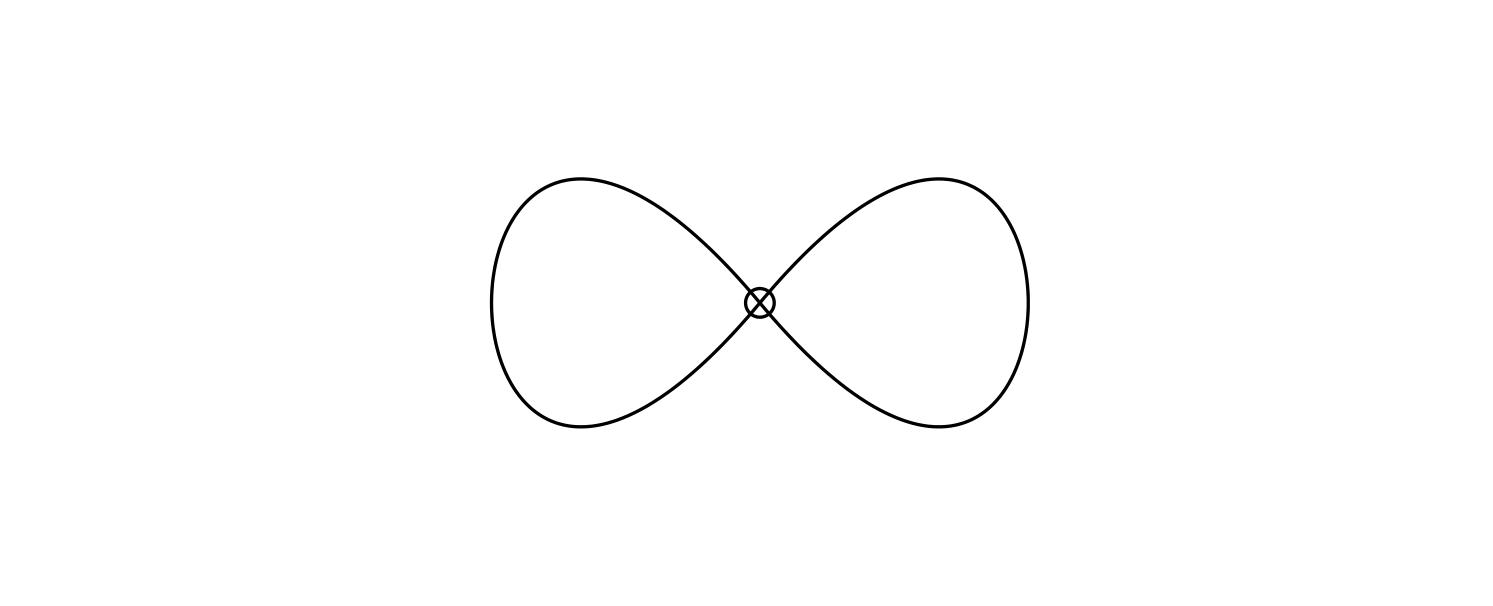
\includegraphics[width=6.32cm]{figures/fig-21.png}
  \caption{（原文无图题）\figorig{84}{21}}
  \label{fig:21}
\end{figure}

\begin{remark} 与有限维情形一样，给出这一定义的另一种方案是假定 $g_i$ 都是形式参数。此时 $\hbar$ 可以取数值，例如 $\hbar=1$，而函数 $\G_n$ 将是 $g_3,g_4,...$ 的一个良定义的幂级数。
\end{remark}

作为例子，考虑自由的有质量理论，即\emph{谐振子}：$U(q)=\frac{m^2q^2}{2}$。此时没有内顶点，因此得到

\begin{proposition} （Wick 定理）当 $n$ 为奇数时 $\G_n(t_1,...,t_n)=0$，并且
$$
\G_{2k}(t_1,...,t_{2k})=\hbar^{k}\sum_{\sigma\in \Pi_k}\prod_{i\in
  \lbrace{1,...,2k
\rbrace}/\sigma}G(t_i-t_{\sigma(i)}).
$$
\end{proposition}

特别地，$\G_2(t_1,t_2)=\hbar G(t_1-t_2)$。
换言之，$\G_2(t_1,t_2)$ 就是（正比于）Green 函数。受此启发，物理学家常把量子场论的一切关联函数都称为 \emph{Green 函数}。

\begin{figure}[htbp]
  \centering
  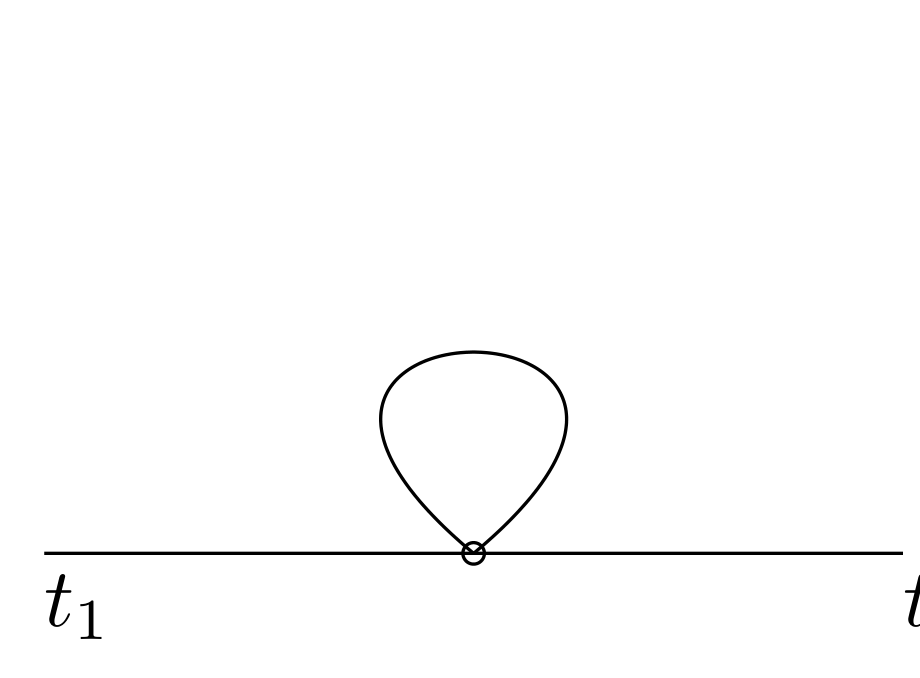
\includegraphics[width=3.89cm]{figures/fig-22.png}
  \caption{（原文无图题）\figorig{85}{22}}
  \label{fig:22}
\end{figure}

\begin{example} 考虑势能 $U(q)=\frac{m^2q^2}{2}-\frac{gq^4}{24}$，
并令 $\hbar=1$。
此时我们来计算两点关联函数模 $g^2$。
换言之，需要算出该函数中 $g$ 的系数。
因此要考虑带两条外边和一个内顶点的 Feynman 图。
这样的图 $\Gamma$ 是唯一的：它由一条边以及附着在其中点的一个圈构成（图 22）。该图的自同构群为 $\Bbb Z/2$。此图的振幅为
$$
F_\Gamma=g\int_{\Bbb R}G(s,t_1)G(s,t_2)G(s,s)ds=
\frac{g}{8m^3}\int_{\Bbb R}e^{-m(|s-t_1|+|s-t_2|)}ds.
$$
由于对 $t_1$ 与 $t_2$ 的对称性，不妨设 $t_1\ge t_2$。把积分拆成三个积分之和，分别取在 $(-\infty,t_2],[t_2,t_1]$ 与 $[t_1,\infty)$ 上，我们得到：
$$
F_\Gamma=
\frac{g}{8m^3}\left(2\int_0^\infty e^{-m(2s+|t_1-t_2|)}ds+|t_1-t_2|e^{-m|t_1-t_2|}\right)=
$$
$$
\frac{g}{8m^4}e^{-m|t_1-t_2|}(1+m|t_1-t_2|).
$$
因此
$$
\G_2(t_1,t_2)=\widetilde{G}(t_1-t_2),
$$
其中
$$
\widetilde{G}(t):=\tfrac{1}{2m}e^{-m|t|}+\tfrac{g}{16m^4}e^{-m|t|}(1+
m|t|)+O(g^2).
$$
这一表达式称为两点函数的\emph{单圈近似}，因为它来自零圈与单圈 Feynman 图。
\end{example} 

\begin{remark} 这里我们考虑的是单个一维粒子的量子力学。
不过，一切都可毫无困难地推广到 $n$ 维粒子或粒子系统的情形（亦即推广为对一维向量值函数而非标量函数的路径积分）。
事实上，若 $q$ 取值于欧氏空间 $V$，则拉格朗日量的二次部分具有形式 $\frac{1}{2}(\dot{q}^2-M(q))$，其中 $M$ 是 $V$ 上的正定二次型。把 $M$ 对角化后，可以假定拉格朗日量的二次部分形如 $\frac{1}{2}\sum_i(\dot{q_i}^2-m_i^2q_i^2)$，这对应于一组相互独立的谐振子。于是在量子理论中传播子将是对角矩阵，其对角元为 $\frac{e^{-m_i|t-s|}}{2m_i}$，而关联函数可按通常的 Feynman 图手续定义。
\end{remark}

\subsection{连通关联函数}

设 $\G^{c}_n(t_1,...,t_n)$ 为\emph{连通关联（或 Green）函数}，其定义为：与 $\G_n(t_1,...,t_n)$ 相同的振幅之和，但只对连通 Feynman 图求和。显然
$$
\G_n(t_1,...,t_n)=\sum_{\lbrace{1,...,n\rbrace}=S_1\sqcup...\sqcup
  S_k} 
\prod \G^c_{|S_i|}(t_j; j\in S_i).
$$
例如，$\G_2(t_1,t_2)=\G_2^c(t_1,t_2)+\G_1^c(t_1)\G_1^c(t_2)$，等等。因此，只要知道连通关联函数，就足以知道关联函数。

\begin{example}\label{harosc} 在自由理论（$U=\frac{m^2q^2}{2}$，即谐振子）中，除 $\G_2$ 以外的一切连通 Green 函数都为零。
\end{example} 

\begin{figure}[htbp]
  \centering
  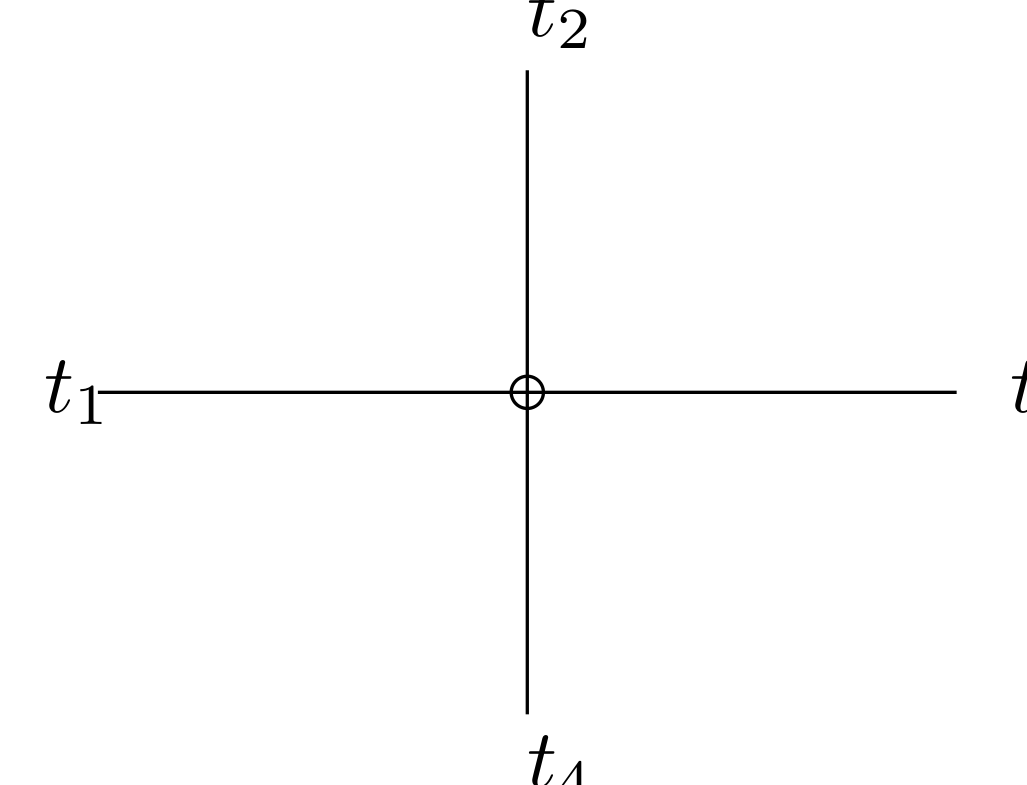
\includegraphics[width=4.35cm]{figures/fig-23.png}
  \caption{（原文无图题）\figorig{86}{23}}
  \label{fig:23}
\end{figure}

\begin{example} 我们来计算上述四次势 $U=\frac{m^2q^2}{2}-\frac{gq^4}{4}$ 所对应理论中的连通四点函数，模 $g^2$。这意味着应当计算带一个内顶点和四条外边的连通 Feynman 图的贡献。这样的图 $\Gamma$ 是唯一的——就是十字形图（带一个内顶点），见图 23。此图没有非平凡自同构。于是
$$
\G_4^c(t_1,t_2,t_3,t_4)=g\int_{\Bbb R}
G(t_1-s)G(t_2-s)G(t_3-s)G(t_4-s)ds+O(g^2).
$$
这个积分可以用初等方法算出；我们把它留作习题。
\end{example} 

\subsection{聚类性质} 
注意 Green 函数 $G(t)$ 在无穷远处趋于零。
这蕴含自由理论关联函数的如下\emph{聚类性质}：
$$
\lim_{z\to \infty} \G_{n}(t_1,...,t_r,t_{r+1}+z,...,t_n+z)=
\G_r(t_1,...,t_r)\G_{n-r}(t_{r+1}...t_n).
$$
此外，容易证明在有相互作用的理论（即带势能的理论）中，就 $\hbar$ 的每一阶而言同样成立（请自行验证！）。聚类性质可以更简洁地写成等式
$$
\lim_{z\to \infty} \G_{n}^c(t_1,...,t_r,t_{r+1}+z,...,t_n+z)=0.
$$
这一性质有物理解释：彼此相距遥远的过程几乎是统计独立的。因此，它可以看作量子场论“具有物理意义”的一个必要条件。

\begin{remark} 尽管如此，确实存在不满足聚类性质、但从物理与数学角度看都很有趣的理论（例如所谓的\emph{拓扑量子场论}；见下文第 \ref{fqm} 小节）。
\end{remark} 

\subsection{配分函数}
设 $J(t)dt$ 是实轴上具有紧支集的测度。考虑“带外源 $J$ 的配分函数”，它是一个形式表达式
$$
Z(J)=\int e^{\frac{-S_E(q) +(J,q)}{\hbar}}Dq.
$$ 
于是我们有形式等式
$$
\frac{Z(J)}{Z(0)}=\sum_n \frac{\hbar^{-n}}{n!}\int_{\Bbb R^n}
\G_n(t_1,...,t_n)J(t_1)...J(t_n)dt_1...dt_n,
$$
与先前一样，我们将把这个等式用作 $Z(J)/Z(0)$ 的定义。于是，知道 $Z(J)/Z(0)$ 等价于知道全部 Green 函数（换言之，$Z(J)/Z(0)$ 是它们的生成函数）。此外，与有限维情形一样，我们有

\begin{proposition} 有
$$
W(J):=\log \frac{Z(J)}{Z(0)}=
\sum_n \frac{\hbar^{-n}}{n!}\int\G_n^c(t_1,...,t_n)J(t_1)...J(t_n)dt_1...dt_n
$$
（亦即 $W$ 是连通 Green 函数的生成函数）。
\end{proposition}

% [Tutor Note: 这里的关键是“归一化”。无穷维路径积分测度 $Dq$ 的归一化因子是无穷大，$Z(0)=\int e^{-S_E/\hbar}Dq$ 本身并不存在（相当于真空图振幅不能求和，参见前文关于“无外顶点分支”的注），可定义的只是比值 $Z(J)/Z(0)$；等价地，$W=\log(Z(J)/Z(0))$ 的展开只含连通图，真空图自动消去。原文坚持写 $Z(J)/Z(0)$ 而非 $Z(J)$，正是为了避开这一乘性无穷大。注意下文在时间紧化到圆上之后，常数函数的积分变为有限，$Z(0)$ 才成为可定义的对象。]

此命题的证明与有限维情形相同。

\begin{remark} 命题的陈述等价于上一小节给出的通常 Green 函数与连通 Green 函数之间的关系。
\end{remark} 

\begin{remark} 我们只能定义那些所有连通分支都至少含一个一价顶点的图的振幅（见上文），这意味着我们实际上既不能定义 $Z(0)$，也不能定义 $Z(J)$，而只能定义它们的比值 $Z(J)/Z(0)$。
\end{remark} 

与有限维情形一样，我们有展开
$$
W(J)=\hbar^{-1}W_0(J)+W_1(J)+\hbar W_2(J)+...,
$$
其中 $W_j$ 是 $j$ 圈贡献（特别地，$W_0$ 由对树的求和给出）。此外，与有限维情形类似，我们对 $W_0$ 与 $W_1$ 有显式公式。

\begin{proposition} 有
$$
W_0(J)=-S_E(q_J)+(q_J,J), 
$$
其中 $q_J$ 是泛函 $S_E^J(q):=S_E(q)-(q,J)$ 的极值点，且在无穷远处衰减。此外，
$$
W_1(J)=-\frac{1}{2}\log \det L_J,
$$ 其中 $L_J$ 是 $V$ 上的线性算子，满足
$$
d^2S_E^J(q_J)(f_1,f_2)=d^2S_E^0(0)(L_Jf_1,f_2).
$$
\end{proposition}

此命题的证明尤其需要说明 $q_J$ 是良定义的，并且 $\det L_J$ 存在。它类似于第 \ref{treepar} 小节中给出的有限维情形同一结果的证明（确切地说，我们当时只证明了零圈情形；但单圈情形的证明是类似的）。因此我们不给出该证明，而宁可用一个例子来说明这一结论。

\begin{example} 设 $U$ 为上文的四次势 $\frac{m^2q^2}{2}+\frac{gq^4}{2}$（为方便起见我们改变了四次项的正负号与归一化），并令 $J(t)=a\delta(t)$。
此时
$$
S_E^J(q)=\int(\tfrac{\dot{q}^2}{2}+U(q))dt-aq(0).
$$ 
欧拉–拉格朗日 方程具有形式
$$
\ddot{q}=m^2q+2gq^3-a\delta(t).
$$
于是函数 $q_J$ 由非线性微分方程
$$
\ddot{q}=m^2q+2gq^3
$$ 
在 $(-\infty,0]$ 与 $[0,\infty)$ 上的两个解 $q_+,q_-$ 连续拼接而成，且在 $0$ 处导数跃变为 $-a$。

我们要求 $q_+,q_-$ 在无穷远处衰减，故它们必须是零能量的解：
$$
E=\frac{\dot{q_\pm}^2}{2}-U(q_\pm)=0.
$$
因此，按 Newton 方程解的标准公式，它们由下述等式确定：
$$
t-t_{\pm}=\int\frac{dq}{\sqrt{2U(q)}}=\int \frac{dq}{mq\sqrt{1+\frac{gq^2}
{m^2}}}=
\frac{1}{2m}\log\frac{\sqrt{1+\frac{gq^2}{m^2}}-1}
{\sqrt{1+\frac{gq^2}{m^2}}+1}.
$$
经过计算可得
$$
q_J(t)=\frac{2mg^{-\frac{1}{2}}}{C^{-1}e^{m|t|}-Ce^{-m|t|}},
$$
其中 $C$ 是方程
$$
\frac{C(1+C^2)}{(1-C^2)^2}=\frac{ag^{\frac{1}{2}}}{4m^2}
$$
的解，它由 $a$ 的幂级数给出且常数项为零。由此用初等方法（但稍嫌冗长）可以算出 $W_0=-S_E^J(q_J)$。

现在，算子 $L_J$ 由下述公式给出
$$
L_J=1+\frac{gA^{-1}\circ q_J(t)^2}{2},
$$ 
其中 $A=-\frac{d^2}{dt^2}+m^2$。因此 $\det L_J$ 是有意义的。事实上，算子 $A^{-1}\circ q_J(t)^2$ 是积分算子，其核为
$$
K_J(x,y):=\frac{e^{-m|x-y|}q_J(y)^2}{2m},
$$ 
它在无穷远处指数衰减；因此算子 $1+\frac{gA^{-1}\circ q_J(t)^2}{2}$ 的行列式是良定义的。
\end{example}

\begin{remark} 在这些计算中，$g, a$ 是形式变量，但只要 $ga^2+m^2>0$，上述计算实际上对这些变量的实数值也成立。
\end{remark} 

\subsection{单粒子不可约 Green 函数}

用 $\G^{1PI}_n(t_1,...,t_n)$ 表示\emph{单粒子不可约（1PI）Green 函数}，亦即与通常 Green 函数相同的振幅之和，但只对单粒子不可约 Feynman 图求和。再定义\emph{截腿}（amputated）单粒子不可约 Green 函数：$\G^{1PIa}_n:=A^{\otimes n}\G^{1PI}_n$
（它由同样的振幅之和定义，只是在每条外边上不写 $G(t_i-s_j)$，而写 $\delta(t_i-s_j)$）。

设 $S_{\rm eff}(q)$ 是 $\G_n^{1PIa}$ 的生成函数，即
$$
S_{\rm eff}(q)=\sum_n\frac{\hbar^{-n}}{n!}\int
\G^{1PIa}_n(t_1,...,t_n)
q(t_1)...q(t_n)dt_1...dt_n.
$$

\begin{proposition} 函数 $W(J)=\log(Z(J)/Z(0))$
是 $S_{\rm eff}(q)$ 的 Legendre 变换，即它等于
$-S_{\rm eff}(\widetilde q_J)+(J,\widetilde q_J)$，其中 $\widetilde q_J$ 是
$-S_{\rm eff}(q)+(J,q)$ 的极值点，且在无穷远处衰减。
\end{proposition}

此命题的证明与有限维情形相同。该命题表明，
为了知道 Green 函数，“只需”知道
截腿单粒子不可约 Green 函数
（通常 Green 函数的生成函数可由 1PI Green 函数的生成函数经
Legendre 变换与指数化重构出来）。
这是个好消息，因为 1PI 图比一般的连通图少得多。

\subsection{动量空间积分}

我们已经看到，Feynman 图的振幅由维数等于内顶点个数的空间上的积分给出。这有时并不方便，
因为即便是树图，这类积分也可能相当复杂。然而，一旦转到 Fourier 变换，
Feynman 积分就会简化，特别是连通图的积分重数等于圈数（于是树图根本不需要积分）。

具体做法如下。
我们不用时间变量 $t$，而考虑其对偶的能量变量 $E$。具有紧支集的函数
$q(t)$ 将用它的 Fourier 变换 $\widehat q(E)$ 代替。
于是由 Plancherel 定理，对实函数
$q_1,q_2$ 有
$$
(q_1,q_2)=\int_{\Bbb R}q_1(t)q_2(t)dt=\int_{\Bbb R} \widehat q_1(E)\overline{\widehat q_2(E)}dE=
\int_{\Bbb R} \widehat q_1(E)\widehat q_2(-E)dE.
$$
这表明传播子由下式给出：
$$
B^{-1}(f,f)=\int_{\Bbb R} \frac{1}{E^2+m^2}\widehat f(E)\widehat f(-E)dE.
$$
位于 $k$ 价顶点处的顶点张量原为 $\delta_{s_1=...=s_k}$，因此将被替换为 $\delta_{Q_1+...+Q_k=0}$，其中 $Q_i$ 是与 $s_i$ 对偶的变量。

\begin{remark} （关于术语）物理学家把时间变量 $t_i,s_j$ 称为\emph{位置变量}，
把能量变量 $E_i,Q_k$ 称为\emph{动量变量}，因为在相对论力学中
（这正是我们研究场论时所处的框架），时间与位置之间、能量与动量之间并无区别
（这是 Lorentz 群作用的结果）。
\end{remark}

这表明，对于给定的、带 $n$ 个外顶点的连通 Feynman 图 $\Gamma$，
其“动量空间”Feynman 规则如下。

1. 给图 $\Gamma$ 定向，使所有外边的方向朝内。

2. 给每条外线（外边）赋变量 $E_i$，给每条内线（内边）赋变量 $Q_j$。这些变量满足
“第一 Kirchhoff 定律”的线性方程：
在每个内顶点处，流入边对应的变量之和等于流出边对应的变量之和。
设 $Y(\bold E)$ 为这些方程的解 $\bold Q$ 构成的空间（它依赖于 $\Gamma$，但我们不显式写出这种依赖）。容易证明，该空间非空仅当 $\sum_i E_i=0$ 时成立，而在这种情况下 $\dim Y(\bold E)$ 等于 $\Gamma$ 的圈数（请证明这一点！）。

3. 在每条外边上写 $\frac{1}{E_i^2+m^2}$，在每条内边上写 $\frac{1}{Q_k^2+m^2}$。
令 $\phi_\Gamma(\bold E,\bold Q)$ 为这些函数的乘积。

4. 把 $\Gamma$ 的\emph{动量空间振幅}定义为分布 $\widehat F_\Gamma(\bold E):$
$$
\widehat F_\Gamma(E_1,...,E_n)=
\prod_jg_{v(j)}
\int_{Y(\bold E)}\phi_\Gamma(\bold E,\bold Q)d\bold Q\cdot \delta(E_1+...+E_n)d\bold E,
$$
它支撑在超平面 $\sum_i E_i=0$ 上。
显然该分布不依赖于 $\Gamma$ 的定向。

\begin{remark} 这里我们须规定空间 $Y(\bold E)$ 上（平移不变的）Lebesgue 测度  $d\bold Q$ 
的归一化。其定义方式是：使 $Y(\bold E)/Y_{\Bbb Z}(0)$ 的体积为 $1$，其中 $Y_{\Bbb  Z}(0)$ 是 $Y(0)$ 中整数元素的集合。因此，若 $T\subset \Gamma$ 是一棵生成树，则在 $Y(\bold E)$ 的坐标 $\lbrace Q_e,e\notin T\rbrace$ 下，
有 $d\bold Q=\prod_{e\notin T}dQ_e$。
 \end{remark} 

% [Tutor Note: 这里的归一化约定最容易出错：$d\bold Q$ 并不是由 $\Bbb R^{\#\text{内边}}$ 上的坐标体积直接诱导的，而是要求基本胞腔 $Y(\bold E)/Y_{\Bbb Z}(0)$ 的体积为 $1$（把整数格点的基本域归一到单位体积）；等价地，沿生成树 $T$ 取独立圈变量时有 $d\bold Q=\prod_{e\notin T}dQ_e$，此即“第一 Kirchhoff 定律”把圈变量与树变量分开的标准做法。原文的 Fourier 变换采用不含 $2\pi$ 的约定（见 $1/(E^2+m^2)=\int G(t)e^{iEt}dt$ 与 $G(t)=e^{-m|t|}/(2m)$），即把 $2\pi$ 吸收进了测度；与常见的 $1/(2\pi)\int$ 约定相比，每个圈积分少一个 $(2\pi)^{-1}$ 因子，与场论章节的约定核对时必须统一。]

现在我们有

\begin{proposition}
函数 $F_\Gamma(\delta_{t_1},...,\delta_{t_n})$ 的 Fourier 变换是
$\widehat F_\Gamma(E_1,...,E_n)$。
因此，连通 Green 函数的 Fourier 变换为
\begin{equation}\label{defcor1}
\widehat\G_n^c(E_1,...,E_n)=
\sum_{\Gamma\in G_{\ge 3}^*(n)}\frac{\hbar^{b(\Gamma)}}{|{\rm Aut}(\Gamma)|}
\widehat F_\Gamma(E_1, \ldots, E_n).
\end{equation}
\end{proposition}

此命题的证明是直接的。

为说明该命题，考虑一个例子。

\begin{example}
四次势的连通四点函数模 $g^2$ 在动量空间中形如：
$$
\widehat \G_4^c(E_1,E_2,E_3,E_4)=
g\prod_{i=1}^4\frac{1}{E_i^2+m^2}\delta(\sum_i E_i)d\bold E+O(g^2).
$$
\end{example}

\begin{figure}[htbp]
  \centering
  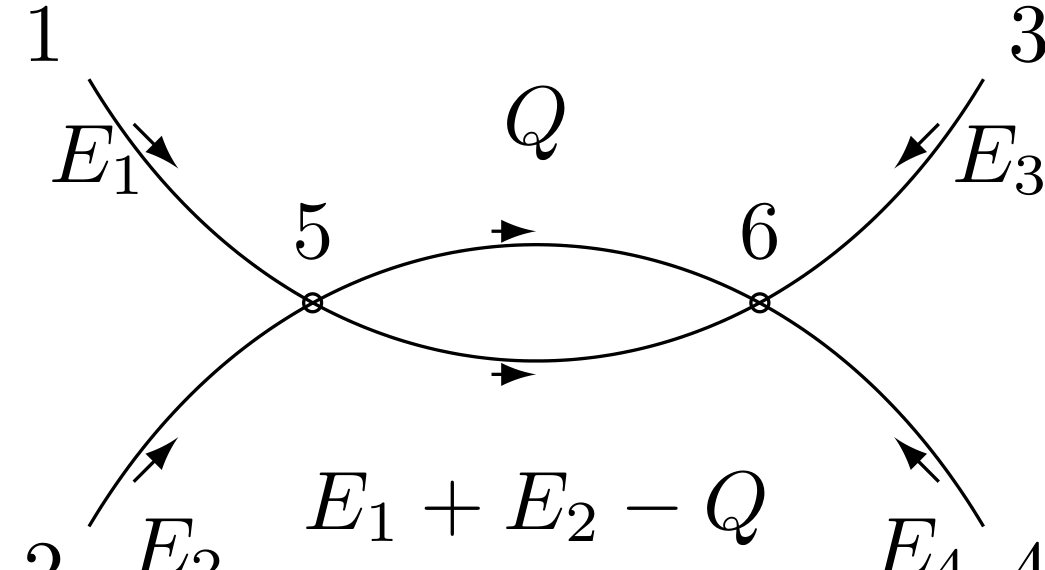
\includegraphics[width=4.42cm]{figures/fig-24.png}
  \caption{（原文无图题）\figorig{92}{24}}
  \label{fig:24}
\end{figure}

\begin{example} 我们来计算同一问题中的 1PI 四点函数，但现在模 $g^3$。因此，除上述项之外，还需算出 $g^2$ 系数，它来自单圈图。这样的图共有三个，彼此相差外边的置换。其中一个图如下：它有外顶点 $1,2,3,4$ 和内顶点 $5,6$，使得 $1,2$ 连接到 $5$，$3,4$ 连接到 $6$，而 $5$ 与 $6$ 由两条边相连（图 24）。此图的对称群为 $\Bbb Z/2$，故其贡献为
$$
\frac{g^2}{2}\left(\int_{\Bbb R}\frac{dQ}{(Q^2+m^2)((E_1+E_2-Q)^2+m^2)}\right)
\prod_{i=1}^4\frac{1}{E_i^2+m^2}\delta(\sum_i E_i)d\bold E.
$$
其中的积分容易算出，例如用留数法。这给出
$$
\widehat \G_4^c(E_1,E_2,E_3,E_4)=
$$
$$
g\prod_{i=1}^4\frac{1}{E_i^2+m^2}
\left(1+\frac{\pi
  g}{m}\sum_{i=2}^4\frac{1}{(E_1+E_i)^2+4m^2}\right)\delta(\sum_i E_i)d\bold E+
O(g^3)
$$
（该式关于 $E_1,E_2,E_3,E_4$ 是对称的，因为当 $\sum_i E_i=0$ 时，对互不相同的 $i,j,k,\ell$ 有
$(E_i+E_j)^2=(E_k+E_\ell)^2$）。
\end{example}

\subsection{动量空间中的 Wick 转动}

为了得到量子力学的关联函数，我们应在欧氏框架下算出它们之后，再把它们 Wick 转动回 Minkowski 框架。我们现在就在动量空间的 Feynman 积分层面上做这件事。（在位置空间做也可以，但就今后的需要而言，在动量空间做更有启发性，因为我们稍后要讨论的高维场论中，动量空间表示更为方便。）

考虑欧氏传播子
$$
\frac{1}{E^2+m^2}=\int_{\Bbb R} G(t)e^{iEt}dt,
$$
其中 $G$ 是 Green 函数。
当我们解析延拓回 Minkowski 框架时，必须在关联函数中把时间变量 $t$ 换成 $e^{i\theta}t$，其中 $\theta$ 从 $0$ 变到 $\frac{\pi}{2}$。特别地，Green 函数 $G(t)$ 必须换成 $G(e^{i\theta}t)$。因此我们必须考虑
$$
\int_{\Bbb R} G(e^{i\theta}t)e^{iEt}dt=
e^{-i\theta} \int_{\Bbb R} G(t)e^{ie^{-i\theta}Et}dt=
\frac{e^{-i\theta}}{e^{-2i\theta}E^2+m^2}.
$$
当 $\theta\to \frac{\pi}{2}$ 时，该函数（作为分布）趋于函数
$\lim_{\varepsilon\to
0+}\frac{i}{E^2-m^2+i\varepsilon}$。
为简洁起见，通常省略极限号，把这个分布写成 $\frac{i}{E^2-m^2+i\varepsilon}$。

由此可见，为了在 Minkowski 框架下计算动量空间中的关联函数，我们应使用与欧氏框架相同的 Feynman 规则，只需把置于边上的传播子换成
$$
\frac{i}{E^2-m^2+i\varepsilon}.
$$
例如，图 24 所示图的贡献为
\scriptsize
$$
-\frac{g^2}{2}\left(\int_{\Bbb R}\frac{dQ}{(Q^2-m^2+i\varepsilon)
((E_1+E_2-Q)^2-m^2+i\varepsilon)}\right)
\prod_{j=1}^4\frac{1}{E_j^2-m^2+i\varepsilon}\delta(\sum_i E_j)d\bold E.
$$
\normalsize

\subsection{圆上的量子力学} 

（至少在数学上）考虑把时间轴换成长度为 $L$ 的圆周情形的欧氏量子力学路径积分是合理的，即 $t\in \Bbb R/L\Bbb Z$（这对应于势场中的一个布朗粒子被条件限制为在给定时间 $L$ 内回到原位置）。
此时理论不变，只是 Green 函数 $G(t)$ 被换成方程 $(-\frac{d^2}{dt^2}+m^2)f=\delta(t)$ 在圆上的周期解 $G_L(t)$。该解具有形式
\begin{equation}\label{glformula} 
G_L(t)=\sum_{k\in \Bbb
  Z}G(t-kL)=\frac{e^{-m(t-\frac{L}{2})}+e^{-m(\frac{L}{2}-t)}}{2m(e^{\frac{mL}{2}}-e^{-\frac{mL}{2}})},\ 0\le t\le L.
\end{equation} 
我们注意到，在圆周情形下，没有外边的图不再引起麻烦（因为常数函数在圆上的积分是收敛的），因此不仅可以定义关联函数（即 $Z(J)/Z(0)$），还可以定义 $Z(0)$ 本身。具体说来，设
$$
U(q)=\frac{m^2q^2}{2}+\sum_{n\ge 3}\frac{g_nq^n}{n!},
$$ 
并令 $m^2=m_0^2+g_2$（其中 $g_i$ 是形式参数）。
于是比值 $Z_{m_0,\bold
  g,L}(0)/Z_{m_0,0,L}(0)$ 是有意义的
（其中 $Z_{m,\bold g,L}(0)$ 表示在指定参数值下的配分函数；此后将省略自变量 $0$）。

事实上，这个比值由下述公式定义：
$$
\frac{Z_{m_0,\bold g,L}}{Z_{m_0,0,L}}=
\sum_{\Gamma\in G_{\ge 2}(0)}\frac{\hbar^{b(\Gamma)}}{|{\rm Aut}(\Gamma)|}
F_\Gamma
$$
（其中 $G_{\ge 2}(0)$ 是没有外顶点、且所有顶点价数 $\ge 2$ 的 Feynman 图之集），而这是一个良定义的表达式。

在情形
$$
g_2=a,\ g_3=g_4=...=0.
$$ 
下计算这一表达式是有启发性的。
此时只有二价顶点，故仅有的连通 Feynman 图是 $N$ 边形，它们都是单圈的。
因此
$$
\log \frac{Z_{m_0,\bold g,L}}{Z_{m_0,0,L}}=
W_1=-\frac{1}{2}\log \det M,
$$
其中
$$
M=1+a(-\tfrac{d^2}{dt^2}+m_0^2)^{-1}.
$$ 
这个行列式可以通过考察本征值来计算。具体说来，$-\frac{d^2}{dt^2}+m_0^2$ 在空间 $C^\infty(\Bbb R/L\Bbb Z)$ 中的本征函数是 $e^{\frac{2\pi int}{L}}$，本征值为 $\frac{4\pi^2n^2}{L^2}+m_0^2$。
于是
$$
\det M=\prod_{n\in \Bbb
  Z}\left(1+\frac{a}{\frac{4\pi^2n^2}{L^2}+m_0^2}\right).
$$
因此，利用 欧拉乘积公式
$$
\sinh(z)=z\prod_{n\ge 1} \left(1+\frac{z^2}{\pi^2n^2}\right),
$$
我们得到
$$
\frac{Z_{m_0,\bold g,L}}{Z_{m_0,0,L}}=
\frac{\sinh(\frac{m_0L}{2})}{\sinh(\frac{mL}{2})}.
$$
（请用对 Feynman 图的求和来复核这一结果！）

\begin{remark} 更通俗地说，我们看到 $U=\frac{m^2q^2}{2}$ 的理论的配分函数 $Z$ 具有形式
$\frac{C}{\sinh(\frac{mL}{2})}$，其中 $C$ 是可以任选的常数。
此后我们取 $C=\frac{1}{2}$；稍后（见例 \ref{benchoi}）会看到为什么这一选择更可取。
\end{remark}

\subsection{无质量情形} 
现在考虑无质量情形，$m=0$。此时传播子应由算子 $-\frac{d^2}{dt^2}$ 求逆得到，亦即它应是核为 $G(t-s)$ 的积分算子，其中 $G(t)$ 是满足微分方程
$$
-G''(t)=\delta(t).
$$ 
的偶函数。
这样的解构成一个单参数族：
$$
G(t)=-\frac{1}{2}|t|+C.
$$ 

利用这个函数（无论 $C$ 如何选取），都可以按 Wick 公式定义自由理论的关联函数。

注意函数 $G$ 在无穷远处不衰减。因此这一理论不满足聚类性质（亦即不是“具有物理意义的”）。

在定义相应的相互作用理论（即带非二次势的理论）时也会遇到困难，因为定义 Feynman 图振幅的积分将会发散。这类发散称为\emph{红外发散}，其起因是被积函数在大时间处不衰减（或者说，在动量空间中它在低频处不正则）。

\subsection{圆值量子力学}
现在考虑拉格朗日量相同、但 $q(t)$ 取值于半径为 $r$ 的圆周 $\Bbb R/2\pi r\Bbb Z$ 的理论（即“sigma 模型”）。至少经典地可以这样做，因为拉格朗日量 $\frac{\dot{q}^2}{2}$ 在此情形下有意义。

我们来定义相应的量子理论。
与线值情形的根本区别在于：既然 $q(t)$ 是圆值的，我们就不应再考虑通常的关联函数
$\langle q(t_1)...q(t_n)\rangle$，而应考虑指数函数的关联函数
$\langle e^{\frac{ip_1q(t_1)}{r}}...e^{\frac{ip_nq(t_n)}{r}}\rangle$，其中 $p_j$ 为整数。它们应由路径积分
\begin{equation}\label{expon}
\int e^{\frac{ip_1q(t_1)}{r}}...e^{\frac{ip_nq(t_n)}{r}}e^{-\frac{S(q)}{\hbar}}Dq,
\end{equation}
定义，其中 $S(q):=\frac{1}{2}\int \dot{q}^2dt$，并约定 $\int e^{-\frac{S(q)}{\hbar}}Dq$ 等于 $1$。
注意只需考虑 $\sum_j p_j=0$ 的情形，否则沿圆周的平移群在被积函数上非平凡地作用，从而在任何合理的定义下该积分都应为零。

现在我们来定义积分 (\ref{expon})。
由于该积分在沿目标圆周的平移下不变，我们不妨设想积分是在 $q:\Bbb R\to \Bbb R$ 且 $q(0)=0$ 上进行的。
下面利用有限维类比。
按照这一类比，通过配方我们将得到
$$
\int e^{\frac{ip_1q(t_1)}{r}}...e^{\frac{ip_nq(t_n)}{r}}e^{-\frac{S(q)}{\hbar}}Dq=
e^{-\frac{\hbar}{2r^2} B^{-1}(\sum_j p_jq(t_j),\sum_j p_jq(t_j))}=
$$
$$
e^{-\frac{\hbar}{2r^2}\sum_{j,\ell} p_\ell p_j G(t_\ell-t_j)}=
e^{\frac{\hbar}{2r^2}\sum_{\ell<j} p_\ell p_j|t_\ell-t_j|},
$$
其中 $B(q,q):=\int \dot{q}^2dt$。
因此，自然地把关联函数定义为
$$
\langle e^{\frac{ip_1q(t_1)}{r}}...e^{\frac{ip_nq(t_k)}{r}}\rangle
=e^{\frac{\hbar}{2r^2}\sum_{\ell<j} p_\ell p_j|t_l-t_j|}.
$$
我们注意到，这一理论与线值情形不同，它\emph{确实}满足聚类性质。事实上，
若 $\sum p_j=0$（如我们所假定的），则
（假定 $t_1\ge t_2\ge...\ge t_n$）有
$$
\sum_{\ell<j}p_\ell p_j(t_\ell-t_j)=
\sum_{j=1}^{n-1}(t_j-t_{j+1})(p_{j+1}+...+p_n)(p_1+...+p_j)=
$$
$$
-\sum_j (t_j-t_{j+1})(p_1+...+p_j)^2,
$$ 
于是聚类性质可由 $(p_1+...+p_j)^2\ge 0$ 推出。

\subsection{圆上的无质量量子力学} 

现在考虑拉格朗日量为 $\frac{\dot{q}^2}{2}$、$q$ 是长度为 $L$ 的圆周上的函数的理论。此时，
按照 Feynman 的通行手法，
我们必须在圆 $\Bbb
R/L\Bbb Z$ 上求算子 $-\frac{d^2}{dt^2}$ 的逆，或等价地解微分方程
$-G''(t)=\delta(t)$。这里遇到了麻烦：
算子 $-\frac{d^2}{dt^2}$ 不可逆，因为它有本征函数 $1$、本征值 $0$；相应地，所讨论的微分方程无解，因为 $\int G''dt$
必须为零，故 $-G''(t)$ 不可能等于 $\delta(t)$
（可以说，指数中的二次型是退化的，
因此高斯积分变得没有意义）。
这个问题可以用下述“杀掉零模”的技巧解决。
具体说来，我们在空间
$\lbrace{q\in C^\infty(\Bbb R/L\Bbb Z): 
\int qdt=0\rbrace}$ 上求算子 $-\frac{d^2}{dt^2}$ 的逆（这可以解释为
在这个余维一的子空间上积分，二次型在其上非退化）。这意味着要求解微分方程
$-G''(t)=\delta(t)-\frac{1}{L}$，并满足 $\int Gdt=0$。
这样的解确实是唯一的，它等于
\begin{equation}\label{greefu} 
G(t)=\frac{(t-\frac{L}{2})^2}{2L}-\frac{L}{24},
\end{equation}
$t\in [0,L]$。于是例如
$\langle q(0)^2\rangle=\frac{L}{12}$。 

更高阶的关联函数按通常方式定义。
此外，可以用标准的 Feynman 图手续定义带任意势的理论。

\subsection{圆上的圆值量子力学} 
最后，考虑同一理论的圆值版本。于是积分变量是映射 $q: \Bbb R/L\Bbb
Z\to \Bbb R/2\pi r\Bbb Z$。这样就出现了新特征——
映射按映射度分成不同的同伦类。我们先考虑对映射度为零的映射积分。
此时应按 $t\in \Bbb
R$ 的情形同样论证，并作如下定义：
$$
\langle e^{\frac{ip_1q(t_1)}{r}}...e^{\frac{ip_nq(t_n)}{r}}\rangle_0:=
e^{-\frac{\hbar}{2r^2}\sum_{\ell,j}p_\ell p_j G(t_\ell-t_j)},
$$
其中 $\sum_j p_j=0$。
（这里下标 $0$ 表示映射度为零的映射）。
假定 $0\le t_1,...,t_n\le L$，利用 \eqref{greefu} 作简短计算可得
$$
\langle e^{\frac{ip_1q(t_1)}{r}}...e^{\frac{ip_nq(t_n)}{r}}\rangle_0
=e^{\frac{\hbar}{2r^2}(\sum_{\ell<j} p_\ell p_j |t_\ell-t_j|+\frac{(\sum_j p_jt_j)^2}{L})}
$$
（当 $L\to \infty$ 时第二项消失，从而回到直线上的答案）。

然而，更为自然的做法（我们稍后就会看到）是对所有映射 $q$ 积分，而不只对映射度为零的映射积分。具体说来，设 $N$ 为整数。
则所有映射度为 $N$ 的映射都具有形式
$q(t)+\frac{2\pi rNt}{L}$，其中 $q$ 是映射度为零的映射。因此，若要对映射度为
$N$ 的映射积分，就应计算与映射度为零时相同的积分，
但作平移 $q\mapsto q+\frac{2\pi r Nt}{L}$。
然而容易看出，这一平移只是把被积函数乘上因子 $e^{\frac{2\pi iN}{L}\sum_j
p_jt_j-\frac{2\pi^2r^2N^2}{\hbar L}}$。因此，对所有映射的积分应由下述公式定义：
$$
\langle e^{\frac{ip_1q(t_1)}{r}}...e^{\frac{ip_nq(t_n)}{r}}\rangle=
$$
\begin{equation}\label{thetform}
e^{\frac{\hbar}{2r^2}(\sum_{l<j} p_\ell p_j |t_\ell-t_j|+\frac{(\sum p_jt_j)^2}{L})}
\frac{\sum_{N\in \Bbb Z}e^{\frac{2\pi iN}{L}\sum_j
p_jt_j-\frac{2\pi^2r^2N^2}{\hbar L}}}
{\sum_{N\in \Bbb Z}e^{-\frac{2\pi^2r^2N^2}{\hbar L}}}.
\end{equation}
引入椭圆 theta 函数
$$
\theta(u,T):=\sum_{N\in \Bbb Z}e^{2\pi iuN-\pi TN^2}.
$$
于是对 $L\ge  t_1\ge...\ge t_n\ge 0$，公式 \eqref{thetform} 
可以改写为
\begin{equation}\label{thetaf}
\langle e^{\frac{ip_1q(t_1)}{r}}...e^{\frac{ip_nq(t_n)}{r}}\rangle
=
e^{\frac{\hbar}{2r^2} (\sum_j (t_{j}-t_{j+1})(p_1+...+p_j)^2+\frac{(\sum_j
p_jt_j)^2}{L})}
\frac{\theta(\frac{\sum_j p_jt_j}{L},\frac{2\pi r^2}{\hbar L})}
{\theta(0,\frac{2\pi r^2}{\hbar L})}.
\end{equation}

% [Tutor Note: 这里按映射度分层求和是本章最值得注意的“拓扑”结构：每一层（映射度为 $N$）的积分与零度积分只差一个显式的指数因子，它来自指数函数在 $q\mapsto q+\frac{2\pi rNt}{L}$ 下的平移；因此对所有映射的积分等于零度积分乘以（theta 函数之比）。所引入的 $\theta(u,T)=\sum_N e^{2\pi iuN-\pi TN^2}$ 正是 Jacobi 第三 theta 函数 $\vartheta_3(u\,|\,iT)$：它的 $N$ 求和可用 Poisson 求和改写为对偶的求和，这正是第 13 章环面配分函数的模不变性与 T 对偶的雏形。注意 $T=\frac{2\pi r^2}{\hbar L}$，$L\to\infty$ 对应 $T\to 0$，此时只有 $N=0$ 项存活，与“直线上只保留零度映射”完全一致；$t_i$ 的排序 $L\ge t_1\ge\cdots\ge t_n\ge0$ 只是把 $|t_\ell-t_j|$ 分段写成求和（与前面聚类性质的计算同一手法）。]

\begin{exercise} 对势能为 $U(q):=\frac{m^2q^2}{2}-\frac{gq^4}{4!}$ 的量子粒子，
在动量空间中计算其单粒子不可约两点函数，模 $g^3$，取 $\hbar=1$。
（我们已在位置空间算过模 $g^2$ 的情形）。
\end{exercise}

\begin{exercise} 设 $U(q):=\frac{m^2q^2}{2}-\frac{gq^3}{3}$。

（i）计算一点函数
${\mathcal G}_1(t)$ 的首项（关于 $g$）。

（ii）计算连通两点函数，模 $g^3$。
\end{exercise} 

\begin{exercise} 
 考虑势能 $U(x):=\frac{m^2\sinh^2(gx)}{2g^2}$。
 当 $J(t)=a\delta(t)$ 时，尽可能显式地给出 $W_0(J)$
（即 $\log(Z(J)/Z(0))$ 的树部分）的公式。
\end{exercise} 

\bigskip
\noindent\rule{\textwidth}{0.6pt}
% [Tutor Note: 本章小结——这一章把路径积分从“形式记号”提升为可操作的定义：先用 Wick 转动把问题搬到欧氏号差，再以 Feynman 图级数定义欧氏关联函数，从而完全绕开无穷维测度；随后证明这些图积分由初等函数组合而成，故解析延拓存在，回到 Minkowski 侧即得带 $i\varepsilon$ 的传播子。三个反复出现的陷阱值得记牢：(1) 归一化——只有比值 $Z(J)/Z(0)$ 可定义，动量空间的 $d\bold Q$ 要按格点的基本域归一，Fourier 变换采用无 $2\pi$ 的约定；(2) 无质量时传播子不衰减，导致聚类性质失效并产生红外发散，圆上还需先处理零模（杀掉常数模、减去 $1/L$）；(3) 时间紧化到圆上会出现按映射度分层的拓扑扇区，圆值场的关联函数由 theta 函数给出，这是第 13 章二维共形场论与 T 对偶的出发点。]



%=====================================================================
% 8  量子力学的算符方法（前半）
% 原文：Section 8. Operator approach to quantum mechanics
%       （arXiv:2409.03117v1, p. 98--111）
%=====================================================================
\section{量子力学的算符方法}

\begin{keytakeaways}
\begin{itemize}
  \item \textbf{物理图像：}经典力学有拉格朗日与哈密顿两套语言，量子力学相应地有路径积分与算子两套语言；本章处理后者，其核心是把相空间上的经典动力学改写为 Hilbert 空间上的算子动力学。
  \item \textbf{数学工具：}有界自伴算子的谱定理（酉等价于乘法算子）、无界算子的可闭性与闭包、伴随算子与边界形式、von Neumann 亏指数，以及由自伴算子生成的强连续单参数酉群。
  \item \textbf{关键结论：}哈密顿量必须实现为（本质）自伴算子，初值问题才适定；自伴扩张的存在性由亏指数是否相等决定，而不同的自伴扩张对应不同的空间边界条件，并可给出完全不同的谱。
  \item \textbf{易错点：}对称不等于自伴；只有本质自伴时闭包才唯一；Poisson 括号升格为对易子时带有因子 $-i/\hbar$，哈密顿方程由此过渡为 Schr\"odinger 方程。
\end{itemize}
\end{keytakeaways}

\bigskip
\noindent\rule{\textwidth}{0.6pt}
\bigskip

在力学与场论（无论经典还是量子）中，有两套主要语言——拉格朗日语言与哈密顿语言。在经典情形，拉格朗日语言是变分学的语言（亦即研究作用量泛函的极值），而哈密顿语言则是辛几何与 哈密顿方程的语言。相应地，在量子情形，拉格朗日语言是路径积分的语言，而哈密顿语言是算子与 Schr\"odinger 方程的语言。我们目前已经研究了前者（至少在微扰展开的意义上），现在转向后者。

\subsection{经典力学中的 哈密顿方程}

我们先回顾经典力学的 哈密顿形式。更多细节可参阅优秀的著作 \cite{A}。

首先回顾经典粒子或粒子系统运动的拉格朗日描述。粒子的位置由位形空间 $X$ 中的一点 $q$ 描述，我们假定 $X$ 是一个流形。系统的拉格朗日量是切丛全空间上的（光滑）函数 ${\mathcal L}: TX\to
\Bbb R$。于是作用量泛函为 $S(q)=\int \mathcal
L(q,\dot{q})dt$。粒子的轨迹是 $S$ 的极值。$q(t)$ 为 $S$ 的极值的条件等价于欧拉–拉格朗日方程（即运动方程），后者在局部坐标下具有形式
$$
\frac{d}{dt}\frac{\partial \mathcal{L}}{\partial \dot{q_i}}=
\frac{\partial \mathcal{L}}{\partial q_i}.
$$
例如，若 $X$ 是 Riemann 流形，且 ${\mathcal L}(q,v)=\frac{v^2}{2}-U(q)$，其中 $U:X\to \Bbb R$ 是势函数，则欧拉–拉格朗日方程就是 Newton 方程
$$
\ddot{q}=-U'(q),
$$
其中 $\ddot{q}=\nabla_{\dot{q}}\dot q$ 是关于 Levi-Civita 联络的协变导数。

现在考虑拉格朗日量为 ${\mathcal L}(q,v)$ 的系统，其关于 $v$ 的微分（固定 $q$）是微分同胚 $T_qX\to T^*_qX$。在上述 Riemann 流形 $X$ 的特殊情形中这当然成立。

\begin{definition}
具有拉格朗日量 ${\mathcal L}$ 的系统的\emph{哈密顿量（或能量函数）}是函数 $H: T^*X\to \Bbb R$，它是 ${\mathcal L}$ 沿纤维的 Legendre 变换；亦即 $H(q,p)=pv_0-{\mathcal L(q,v_0)}$，其中 $v_0$ 是 $pv-{\mathcal L(q,v)}$ 的（唯一）临界点。流形 $T^*X$ 称为\emph{相空间（或状状态空间）}。变量 $p$ 称为\emph{动量变量}。
\end{definition}

例如，若 ${\mathcal L}=\frac{v^2}{2}-U(q)$，则 $H(q,p)=\frac{p^2}{2}+U(q)$。

\begin{remark} 由于 Legendre 变换是对合的，我们也有：拉格朗日量是哈密顿量沿纤维的 Legendre 变换。
\end{remark}

设 $q_i$ 是 $X$ 上的局部坐标。该坐标系给出 $T^*X$ 上的坐标系 $(q_i,p_i)$。我们得到

\begin{proposition}
运动方程等价于\emph{哈密顿方程}
$$
\dot{q_i}=\frac{\partial H}{\partial p_i},\
\dot{p_i}=-\frac{\partial H}{\partial q_i},
$$
其含义是：它们可由 哈密顿方程消去 $p_i$ 而得到。
\end{proposition}

用 Poisson 括号来写 哈密顿方程是很有用的。回顾流形 $T^*X$ 具有典范辛结构 $\omega=d\alpha$，其中 $\alpha$ 是 $T^*M$ 上的典范 1-形式（称为\emph{Liouville 形式}），其构造如下：对任意 $z\in T_{(q,p)}(T^*X)$，
$$
\alpha(z)=(p,d\pi(q,p)z),
$$
其中 $\pi: T^*X\to X$ 是投影。在局部坐标下，我们有
$$
\alpha=\sum_i p_idq_i,\
\omega=\sum_i dp_i\wedge dq_i.
$$

现在设 $(M,\omega)$ 是辛流形（在我们的情形 $M=T^*X$）。由于 $\omega$ 非退化，可以定义 Poisson 双向量 $\omega^{-1}$，它是丛 $\wedge^2TM$ 的一个截面。于是，给定 $M$ 上任意两个光滑函数 $f,g$，可以定义第三个函数——它们的\emph{Poisson 括号}
$$
\lbrace{ f,g\rbrace}=(df\otimes dg,\omega^{-1}).
$$
该运算反对称并满足 Jacobi 恒等式，亦即它是 $C^\infty(M)$ 上的李括号。对于 $M=T^*X$，在局部坐标下有
$$
\lbrace{ f,g\rbrace}=\sum_i\biggl(\frac{\partial f}{\partial
  q_i}\frac{\partial g}{\partial p_i}-
\frac{\partial f}{\partial
  p_i}\frac{\partial g}{\partial q_i}\biggr).
$$

这表明 哈密顿方程可以用 Poisson 括号写成如下形式：
\begin{equation}\label{heobs}
\frac{d}{dt}f(q(t),p(t))=\lbrace{f,H\rbrace}(q(t),p(t)).
\end{equation}
对任意光滑函数（“经典可观测量”）$f\in C^\infty(T^*X)$ 成立；或者简写为
$$
\frac{df}{dt}=\lbrace f,H\rbrace.
$$
换言之，哈密顿方程说的是：$f$ 的观测值的变化率等于 $\lbrace{f,H\rbrace}$ 的观测值。

\subsection{无界自伴算子}

量子力学在哈密顿框架下的严格数学处理，建立在 von Neumann 关于 Hilbert 空间中无界自伴算子的理论之上。我们回顾该理论的基础。

\subsubsection{有界自伴算子的谱定理}
设 $\mathcal H$ 是可分复 Hilbert 空间，内积为 $\la,\ra$（对第一个变量反线性，这是量子物理中的传统约定）。我们首先回顾有界自伴算子 $A: \mathcal H\to \mathcal H$ 的\emph{谱定理}，它推广了 Hermitian 矩阵的对角化定理。

\begin{theorem}\label{specthe} (von Neumann) 设 $A$ 是有界自伴算子。则存在测度空间 $(X,\mu)$、本性有界可测函数 $h: X\to \Bbb R$ 以及等距同构 $\mathcal H\to L^2(X,\mu)$，使得在该等距同构下 $A$ 对应于乘以 $h$ 的乘法算子。此外，谱 $\sigma(A)$ 是使集合 $h^{-1}(\lambda-\varepsilon,\lambda+\varepsilon)$ 对每个 $\varepsilon>0$ 都具有正测度（即 $\mu(h^{-1}(\lambda-\varepsilon,\lambda+\varepsilon))>0$）的 $\lambda\in \Bbb R$ 之集；而 $A$ 的本征值（若存在）是满足 $\mu(h^{-1}(\lambda))>0$ 的 $\lambda\in \Bbb R$，其本征函数是 $h^{-1}(\lambda)$ 的具有正测度的子集的指示函数。
\end{theorem}

\subsubsection{可闭算子与闭算子}
现在转向不一定有界的算子。设 $\mathcal H'$ 是另一个可分 Hilbert 空间。$\mathcal H$ 上的\emph{稠定线性算子}是一对 $(A,V)$，其中 $V\subset \mathcal H$ 是稠密子空间，$A$ 是（可能无界的）线性算子 $V\to \mathcal H'$。空间 $V$ 称为 $A$ 的\emph{定义域}；在记号中我们常常省略它，只用 $A$ 表示该算子。这样的算子 $A$ 有图 $\Gamma_A\subset V\times \mathcal H'\subset \mathcal H\times \mathcal H'$。设 $\overline \Gamma_A$ 是 $\Gamma_A$ 在 $\mathcal H\times \mathcal H'$ 中的闭包。若 $(0,u)\in \overline \Gamma_A$（其中 $u\in \mathcal H'$）蕴含 $u=0$，即第一投影 $p_1:\overline\Gamma_A\to \mathcal H$ 是单射，则称 $A$ 是\emph{可闭的}。此时令 $\overline V:=p_1(\overline \Gamma_A)\subset \mathcal H$，则 $V\subset \overline V$，并得到算子 $A: V\to \mathcal H'$ 到稠定算子 $\overline A: \overline V\to \mathcal H'$ 的延拓，称之为 $A$ 的\emph{闭包}。若 $A$ 可闭且 $\overline A=A$，则称 $A$ 是\emph{闭的}；换言之，$A$ 闭当且仅当它在 $\mathcal H\times \mathcal H'$ 中的图是闭的。显然，对任何可闭的 $A$，其闭包 $\overline A$ 都是闭的。此外，若 $A$ 有界，则它可闭，$\overline V=\mathcal H$，且 $\overline A: \mathcal H\to \mathcal H'$ 就是 $A$ 的连续（=有界）延拓。

然而一般而言，稠定算子未必可闭。例如，若 $\mathcal H'$ 是有限维的而 $A: V\to \mathcal H'$ 无界，则存在序列 $v_n\in V$ 使 $v_n\to 0$ 但 $||Av_n||\ge 1$。于是序列 $w_n:=\frac{v_n}{||Av_n||}$ 趋于 $0$，而 $||Aw_n||=1$；由于 $\mathcal H'$ 中的单位球面紧，必要时取子列，可设 $Aw_n\to u$，其中 $u\in \mathcal H'$ 且 $||u||=1$。于是 $(0,u)\in \overline{\Gamma}_A$，故 $A$ 不可闭。由此可见，$A$ 可闭当且仅当它是有界的。

另一方面，若 $\mathcal H'$ 是无限维的，则存在重要的无界可闭算子类。例如考虑 $\mathcal H=\mathcal H'$ 的情形。称算子 $A: V\to \mathcal H$ 为\emph{对称的}，若对一切 $v,w\in V$ 有 $\la v,Aw\ra=\la Av,w\ra$。我们断言每个对称算子都可闭，且其闭包是对称的。事实上，设 $(v_n,Av_n)\to (0,u)$，$u\in\mathcal H$。取序列 $u_k\in V$ 使 $u_k\to u$。则
$$
\la Au_k,v_n\ra=\la u_k,Av_n\ra\to \la u_k,u\ra,\ n\to \infty.
$$
但最左端的表达式趋于零，故对一切 $k$ 有 $\la u_k,u\ra=0$，从而 $||u||^2=0$，即 $u=0$，因此 $A$ 可闭。此外，对任意 $v,w\in \overline V$，存在序列 $v_n\to v,w_n\to w$（均在 $V$ 中）使得 $Av_n\to \overline Av$，$Aw_n\to \overline Aw$，于是
$$
\la v,\overline Aw\ra=\lim_{n\to \infty}\la v_n,Aw_n\ra=\lim_{n\to \infty}\la Av_n,w_n\ra=\la \overline Av,w\ra,
$$
故 $\overline A$ 对称。

\subsubsection{伴随算子}
然而，仅有闭对称算子对量子力学来说还不够，因为这样的算子一般不能对角化。我们需要的是\emph{自伴}算子，即满足一个重要的附加性质的闭对称算子。为表述这一性质，首先需要定义伴随算子的概念。

设 $(A,V)$ 是闭对称算子。用 $V^\vee$ 记满足如下条件的 $u\in \mathcal H$ 构成的空间：线性泛函 $v\mapsto \la u,Av\ra$ 在 $V$ 上有界。此时由 Riesz 表示定理，存在唯一的向量 $w\in \mathcal H$ 使 $\la u,Av\ra=\la w,v\ra$，且该向量线性依赖于 $u$。于是得到算子 $A^\dagger: V^\vee\to \mathcal H$。注意 $V^\vee\supset V$，且 $A^\dagger$ 是 $A$ 到 $V^\vee$ 的延拓，故 $(A^\dagger,V^\vee)$ 是稠定算子，称为 $(A,V)$ 的\emph{伴随算子}。此外，该算子是闭的：若 $(u_n,A^\dagger u_n)\to (u,w)$，则对 $v\in V$，
$$
\la A^\dagger u_n,v\ra=\la u_n,Av\ra\to \la u,Av\ra,\ n\to \infty,
$$
同时 $\la A^\dagger u_n,v\ra\to \la w,v\ra$，故 $\la u,Av\ra=\la w,v\ra$，从而 $u\in V^\vee$ 且 $w=A^\dagger u$。

然而我们将看到，$A^\dagger$ 一般不再对称。因此可以考察 $V^\vee$ 上的斜 Hermitian 形式
$$
B(v,w):=(A^\dagger v,w)-(v,A^\dagger w)
$$
以刻画其非对称性，称之为\emph{边界形式}（之所以这样称呼，是因为在例子中它对应于分部积分产生的边界项）。按定义 $V\subset {\rm Ker}B$（事实上可以证明 $V={\rm Ker}B$，但我们无需此事实）。容易看出，$A$ 的闭对称扩张对应于关于形式 $B$ 的闭迷向子空间 $V\subset L\subset V^\vee$；具体地说，$A$ 到 $L$ 的扩张定义为 $A^\dagger|_L$ 的限制。此外，这样的扩张 $(A^\dagger,L)$ 的伴随算子是 $(A^\dagger, L^\perp)$，其中 $L^\perp$ 是 $L$ 在 $V^\vee$ 中关于 $B$ 的正交补。

\subsubsection{自伴算子}
称闭对称算子 $(A,V)$ 为\emph{自伴的}，若 $V^\vee=V$，即 $A^\dagger=A$。我们看到，$A$ 的\emph{自伴扩张}对应于\emph{拉格朗日}子空间 $L$，即使得 $L=L^\perp$ 的子空间。注意这样的扩张/子空间可能存在也可能不存在：自伴扩张（或拉格朗日子空间）存在的充要条件是 Hermitian 形式 $iB$ 的符号差 $(n_+,n_-)$ 满足 $n_+=n_-$（亦即 $A$ 的所谓\emph{亏指数} $n_\pm \in \Bbb Z_{\ge 0}\cup\infty$ 相等）。然而在量子力学模型中它们通常存在，并对应于各种空间边界条件。

% [Tutor Note: 对称与自伴的分界全在定义域：对称只要求 <Av,w>=<v,Aw> 对 v,w∈V 成立，自伴则还要求 A 的伴随算子（定义在 V^∨ 上）不再扩大定义域，即 V^∨=V。一般地 V⊊V^∨，商空间 V^∨/V 上的边界形式 B 度量这种“缺陷”；闭对称扩张 ↔ V 与 V^∨ 之间 B-迷向的闭子空间 L，自伴扩张 ↔ B-拉格朗日子空间 L=L^⊥。本质自伴（闭包自伴）等价于亏指数 (0,0)，此时自伴扩张唯一。]

称对称算子 $(A,V)$ 为\emph{本质自伴的}，若其闭包 $(\overline A,\overline V)$ 是自伴的。于是本质自伴算子有唯一的自伴扩张，因而拥有这样的算子基本上等同于拥有一个自伴算子。这一概念很方便，例如当我们不想显式描述空间 $\overline V$ 时。

无界自伴算子之所以重要，在于 von Neumann 谱定理可自然地推广到它们。具体地说，定义自伴算子 $(A,V)$ 的\emph{谱} $\sigma(A,V)$ 为使算子 $A-\lambda: V\to \mathcal H$ 不满射的 $\lambda\in \Bbb C$ 的集合。于是有

\begin{theorem} 除 $h$ 本性有界这一陈述之外，定理 \ref{specthe} 对不一定有界的自伴算子同样成立。此外，在其谱定理实现中，$A$ 的定义域 $V$ 是满足 $hg\in L^2(X,\mu)$ 的 $g\in L^2(X,\mu)$ 构成的空间。
\end{theorem}

若测度 $\mu$ 集中在可数集上（即可取 $X=\Bbb N$ 且对 $j\in \Bbb N$ 有 $\mu(j)=1$），则 $\mathcal H$ 有由本征函数组成的基，反之亦然；此时称 $A$ 的谱为\emph{纯点谱}。例如当 $A$ 紧时（Hilbert–Schmidt 定理）就会发生这种情况。另一极端是\emph{纯连续谱}，此时没有本征值（即在谱定理实现中，$X$ 的所有点都是零测度）。谱定理蕴含：任何自伴算子都可唯一地写成两个自伴算子的正交直和，它们分别具有纯点谱与纯连续谱。

谱定理还蕴含如下推论。

\begin{corollary} 设 $(A,V)$ 是自伴算子。则存在唯一的单参数酉算子群 $U(t)=e^{iAt}: \mathcal H\to \mathcal H$，它关于 $t$ 强连续、保持 $V$ 不变并与 $A$ 交换，且对一切 $v\in V$，函数 $t\mapsto U(t)v$ 可微并满足
$$
\frac{d}{dt}(U(t)v)=iAU(t)v.
$$
\end{corollary}

\begin{proof} 利用 $A$ 为乘以 $h: X\to \Bbb R$ 的乘法算子的谱定理实现，可定义 $U(t)$ 为乘以 $e^{ith}$ 的乘法算子。
\end{proof}

事实上，反之亦真：每个强连续单参数群 $U(t)$（即 Lie 群 $\Bbb R$ 在 $\mathcal H$ 上的酉表示）都唯一地（在等距同构意义下）来自某个自伴算子。

\begin{remark} 谱定理蕴含：若 $(A,V)$ 是自伴算子且对某个非零 $v\in V$ 有 $Av=\lambda v$，则 $\lambda\in \Bbb R$。相反，若 $(A,V)$ 只是对称而非自伴，von Neumann 证明了 $A$ 在 $V$ 上的本征值集合或者是（开）上半平面 $\Bbb C_+$（当 $n_+>0,n_-=0$），或者是下半平面 $\Bbb C_-$（当 $n_->0,n_+=0$），或者两者兼有（当 $n_+,n_->0$）。
\end{remark}

\subsubsection{例子}

\begin{example} 考虑 $\mathcal H=L^2(S)$ 上的对称算子 $P:=-i\frac{d}{dx}$，其中 $S:=\Bbb R/2\pi \Bbb Z$（圆周上的动量算子）。该算子在空间 $V:=C^\infty(S)$ 上对称，并且可以证明它在该空间上还是本质自伴的（请验证！）。相应的空间 $\overline V$ 是\emph{Sobolev 空间} $H^1(S)$，由满足 $f'\in L^2(S)$（在分布意义下）的 $f\in L^2(S)$ 组成（注意这样的函数连续）。相应自伴算子的谱为纯点谱且等于 $\Bbb Z$，本征函数为 $e^{inx}$，即 $Pe^{inx}=ne^{inx}$。因此 $A$ 的谱实现是在 $\ell_2(\Bbb Z)$ 上（带计数测度），其中 $P$ 通过乘以函数 $n$ 作用（亦即该实现简单地归结为 $S$ 上函数的 Fourier 展开）。类似地，能量算子 $P^2=-\frac{d^2}{dx^2}$ 在同一空间上本质自伴，但闭包的定义域更小——即由满足 $f''\in L^2(S)$ 的 $f\in L^2(S)$ 组成的 Sobolev 空间 $H^2(S)$。其谱为 $\Bbb Z_{\ge 0}$，本征函数相同：$P^2e^{inx}=n^2e^{inx}$。
\end{example}

\begin{example} 下一个例子更有趣，是自伴扩张理论的典型。考虑同样的动量算子 $P:=-i\frac{d}{dx}$，但如今作用在稠密子空间 $V\subset L^2[0,2\pi]$ 上，该子空间由在区间两端各阶导数均为零的光滑函数组成。此时 $P$ \textbf{不是}本质自伴的：空间 $\overline V$ 是满足 $f(0)=f(2\pi)=0$ 的函数 $f\in H^1[0,2\pi]$ 构成的空间，而 $V^\vee=H^1[0,2\pi]$，且
$$
B(f,g)=i(\overline{f(2\pi)}g(2\pi)-\overline{f(0)}g(0)).
$$
于是在商 $V^\vee/\overline V=\Bbb C^2$ 上我们有
$$
B((a,b),(a,b))=i(|b|^2-|a|^2),
$$
其中 $a=f(0)$，$b=f(2\pi)$。因此 $V^\vee$ 的拉格朗日子空间由满足 $|b|=1$ 的点 $b\in \Bbb C$ 给出；具体地说，它是满足 $f(2\pi)=bf(0)$ 的函数 $f\in H^1[0,2\pi]$ 构成的空间 $L_b$。相应自伴算子的谱仍是纯点谱，因此应在空间 $L_b$ 中寻找本征函数。于是得到本征函数 $e^{i(n+s)x}$，其中 $b=e^{2\pi is}$。所以本征值集合为 $\Bbb Z+s$，可见谱依赖于自伴扩张的选择。

还要注意，任何复数 $\lambda$ 都是对称（非自伴！）算子 $P^\dagger$ 在 $V^\vee$ 上的本征值，本征向量为 $e^{i\lambda x}$。
\end{example}

\begin{example} 现在考虑同样的动量算子 $P:=-i\frac{d}{dx}$，但它作用在紧支撑光滑函数空间 $V=C_0^\infty(\Bbb R)$ 上，这是 $\mathcal H=L^2(\Bbb R)$ 的子空间。此时 $P$ 本质自伴，且 $\overline V=V^\vee$ 是 $H^1(\Bbb R)$ 中由满足 $f'\in L^2(\Bbb R)$ 的 $f\in L^2(\Bbb R)$ 组成的子空间。$P$ 的谱定理实现是 $L^2(\Bbb R)$ 上乘以 $x$ 的乘法算子，这由 Fourier 变换给出。因此该算子的谱为纯连续谱，并构成整个实直线 $\Bbb R$。类似地，算子 $P^2=-\frac{d^2}{dx^2}$ 在 $V$ 上也本质自伴，其自伴扩张具有纯连续谱 $\Bbb R_{\ge 0}$。
\end{example}

\begin{example} 再一次取 $P:=-i\frac{d}{dx}$，但如今作用在 $\mathcal H=L^2(\Bbb R_{\ge 0})$ 的子空间 $V$ 上，它由在 $0$ 处各阶导数均为零的紧支撑光滑函数组成。该算子不是本质自伴的：空间 $\overline V$ 是满足 $f(0)=0$ 的函数 $f\in H^1(\Bbb R_{\ge 0})$ 构成的空间，而 $V^\vee$ 是整个 $H^1(\Bbb R_{\ge 0})$。于是空间 $V^\vee/\overline V$ 是一维的，形式 $B$ 由 $B(f,g)=-i\overline{f(0)}g(0)$ 给出，因此不存在自伴扩张（亏指数不相等：$n_+=1,n_-=0$）。

我们来求 $P$ 在 $V$ 上的本征值。本征值为 $\lambda$ 的本征向量是 $e^{i\lambda x}$，它属于 $V$ 当且仅当 $\lambda\in \Bbb C_+$。因此 $P$ 的本征值集合为 $\Bbb C_+$。
\end{example}

% [Tutor Note: 亏指数的计算：n_± = dim Ker(A^† ∓ i)（在 C_± 内 dim Ker(A^†−λ) 为常数）。本例可逐一验证：e^{iλx}∈L^2(R_{≥0}) 当且仅当 Im λ>0，故 Ker(P^†−i) 由 e^{−x} 张成（一维），而 Ker(P^†+i)=0，即 (n_+,n_-)=(1,0)。这与正文的 remark 相呼应：此时 P 在 V 上的本征值恰为整个上半平面（任意 λ∈C_+ 的 e^{iλx} 都在 V 中）。等价地，iB 在 V^∨/V 上非退化且符号差为 (1,0)，n_+≠n_- 故无自伴扩张。]

\begin{example}\label{harosc1} 设 $A=-\frac{1}{2}\frac{d^2}{dx^2}+\frac{1}{2}x^2$，$V=C^\infty_0(\Bbb R)$（量子谐振子）。则 $A$ 本质自伴，$\overline A$ 具有纯点谱 $n+\frac{1}{2}$，$n\in \Bbb N$，本征向量为 $H_n(x)e^{\frac{x^2}{2}}$，其中 $H_n$ 是 Hermite 多项式（定理 \ref{Hermite}）。
\end{example}

% [Tutor Note: 原文此处把本征向量写成 H_n(x)e^{x^2/2}，疑为笔误：指数取正号时函数在 |x|→∞ 指数增长，不属于 L^2(R)。按第 4 章定理 \ref{Hermite} 的 (ii)(iii)（H_n e^{−x^2/2} 是 L=−(1/2)∂^2+(1/2)x^2 的本征函数并构成 L^2(R) 的正交基），正确写法应为 H_n(x)e^{−x^2/2}；谱 n+1/2 无误。此处保留原文原样。]

\begin{remark} 更一般地，已知：若 $U(x)$ 是 $\Bbb R$ 上分段连续的势，且在 $\pm \infty$ 处趋于 $+\infty$，则算子 $A:=-\frac{1}{2}\frac{d^2}{dx^2}+U(x)$ 在 $V=C^\infty_0(\Bbb R)$ 上本质自伴并具有纯点谱，本征值为 $E_0< E_1\le E_2\le ...$（下面引理 \ref{uniqueeig} 将证明 $E_0$ 总是单本征值，且相应的本征向量是正函数）。
\end{remark}

\begin{example} 设 $M$ 是具有边界 $\partial M$ 的紧 Riemann 流形，$\mathcal H=L^2(M)$，$A=\Delta$ 是 $M$ 上的 Laplace 算子，它作用在由 $M$ 上在边界处连同各阶导数都为零的光滑函数构成的空间 $V$ 上。此时 $\overline V$ 是 Sobolev 空间 $H^2(M)$（即满足 $\Delta f\in L^2(M)$ 的 $f\in L^2(M)$）中在 $\partial M$ 上连同一阶法向导数都为零的函数构成的空间，而 $V^\vee=H^2(M)$。由 Stokes 公式
$$
\int_M (u\Delta v-v\Delta u)dx=\int_{\partial M}(u\partial_{\bold n} v-v\partial_{\bold n}u)d\sigma,
$$
其中 $\bold n$ 表示关于 $\partial M$ 的法向导数，故有
$$
B(f,g)=i\int_{\partial M}(\overline f\partial_{\bold n} g-g\partial_{\bold n} \overline f)d\sigma.
$$
因此若 $\partial M=0$，则算子 $A$ 本质自伴且有唯一自伴扩张；而若 $\partial M\ne 0$，则它不本质自伴，且存在许多自伴扩张，对应于 $\partial M$ 上的各种边界条件。最常见的是 Dirichlet 边界条件 $f=0$ 与 Neumann 边界条件 $\partial_{\bold n} f=0$。当然，与这些条件相联系的谱（总是纯点谱）完全不同。

边界非平凡的最简单例子是 $M=[0,\pi]$，此时 $\dim V^\vee/\overline V=4$，且
$$
B(f,g)=i(\overline {f}g'-\overline{f'}g)|_0^{\pi}.
$$
对于 Dirichlet 边界条件 $f(0)=f(\pi)=0$，得到本征基 $\sin nx$，本征值为 $-n^2$，$n\in \Bbb Z_{\ge 1}$；而对于 Neumann 边界条件 $f'(0)=f'(\pi)=0$，得到本征基 $\cos nx$，本征值同样为 $-n^2$，但此时 $n\in \Bbb Z_{\ge 0}$。

考虑混合边界条件：
$$
f(0)=0,\ f'(\pi)-af(\pi)=0
$$
对某个实数 $a$。则本征函数为 $\sin \lambda x$，其中
$$
\lambda \cos \pi \lambda = a \sin \pi\lambda.
$$
于是本征值为 $-\lambda^2$，其中 $\lambda$ 取遍方程
$$
\lambda\ {\rm cotan} \pi\lambda=a.
$$
的解。例如，在极限 $a\to \infty$ 下我们重新得到 Dirichlet 边界条件的答案。
\end{example}

% [Tutor Note: 原文此处边界形式含因子 i，疑为沿袭动量算符例造成的笔误。按 B(v,w):=(A^†v,w)−(v,A^†w) 及正文的 Stokes 公式，取 A=Δ 直接计算得 B(f,g)=−∫_{∂M}(\bar f∂_n g−g∂_n\bar f)dσ，与原文相差因子 −i；一阶算子 A=−i d/dx 才自然出现因子 i。两种归一化只差非零常数，不影响迷向性与自伴扩张判据。另：下文 “if ∂M=0” 应读作 “∂M 为空集”（无边情形）。两处均保留原文原样。]

\begin{exercise} 设 $H=-\frac{1}{2}\frac{d^2}{dx^2}+a\chi_{[-1,1]}(x)$，其中 $\chi$ 是指示函数，$a\in \Bbb R$，并设它定义在 $V=C^\infty_0(\Bbb R)\subset \mathcal H=L^2(\Bbb R)$ 上。证明 $H$ 本质自伴，并求出其自伴扩张的谱与本征值（分别考虑 $a\ge 0$ 与 $a<0$ 的情形）。

\textbf{提示}：如上所述，谱由使 $H-E: \overline V\to \mathcal H$ 不满射的 $E\in \Bbb R$ 组成。因此尝试对 $f\in \mathcal H$ 求解方程
$$
(H-E)u=f
$$
并将解写成
$$
f(x)=\int_{\Bbb R} G(x,y)dy,
$$
其中 $G(x,y)$ 是方程
$$
(H-E)f=\delta(x-y).
$$
的基本解。你应得到：当 $a\ge 0$ 时没有本征函数（纯连续谱）；而当 $a<0$ 时谱是混合的：既有连续谱，也有一些具有负本征值的本征函数，它们称为\textbf{束缚态}。
\end{exercise}

% [Tutor Note: 提示中的表达式 f(x)=∫_R G(x,y)dy 疑有笔误：G 是 (H−E) 的基本解，正确的解的表示应为 u(x)=∫_R G(x,y)f(y)dy（或对源项作相应的卷积），否则该式既不依赖于给定的 f，也无法由 (H−E)u=f 解出。此处保留原文原样。]

\subsection{量子力学中的哈密顿量}

量子化的要诀（yoga）是说：要量子化流形 $X$ 上的经典力学，需把经典状状态空间 $T^*X$ 替换为量子状状态空间——$X$ 上平方可积复半密度构成的 Hilbert 空间 ${\mathcal H}=L^2(X)$（更确切地说，是相应的射影空间）。其次，需把经典可观测量，即（足够好的）实函数 $f\in C^\infty(T^*X)$，替换为量子可观测量 $\widehat f$；后者是 ${\mathcal H}$ 上（无界、稠定）的算子，一般彼此不对易。于是，可观测量 $A$ 在单位范数状态 $\psi\in \mathcal H$ 中的（期望）值按定义为 $\la\psi,A\psi\ra$（只要它有良好定义）。

算子 $\widehat f$ 应线性依赖于 $f$。此外，它们应依赖一个称为\emph{普朗克常数}的正实参数 $\hbar$，并满足如下关系：
$$
[\widehat{f},\widehat{g}]=i\hbar\widehat{\lbrace{f,g\rbrace}}+O(\hbar^2),\
\hbar\to 0.
$$
由于在量子力学中函数的 Poisson 括号所扮演的角色由算子的对易子承担，该关系表达了“经典力学应是 $\hbar\to 0$ 时量子力学的极限”这一条件。\footnote{注意，映射 $f\mapsto \widehat f$ 不可能满足恒等式 $\widehat{fg}=\widehat f\widehat g$，因为函数乘法可交换而算子乘法不可交换。}

我们必须马上让读者失望地承认：量子化映射 $f\mapsto \widehat f$ 没有典范选择。不过，对于某些特定的 $f$，$\widehat f$ 有一些标准选择，我们下面讨论。

我们限于 $X=\Bbb R$ 的情形，此时相空间上有坐标 $q$（位置）与 $p$（动量）。此时可自然地把半密度视为函数，并有如下标准约定。

1. 当 $f$ 与 $p$ 无关时，$\widehat f=f(q)$（即乘以 $f(q)$ 的乘法算子）。

2. $\widehat{p^m}\to (-i\hbar \frac{d}{dq})^m$。

（注意这些约定满足我们的条件，因为 $[\widehat q,\widehat p]=i\hbar$，而 $\lbrace{q,p\rbrace}=1$。）

\begin{example} 对于上面考虑过的经典哈密顿量 $H=\frac{p^2}{2}+U(q)$，量子化后将得到\emph{Schr\"odinger 算子}
$$
\widehat H=-\frac{\hbar^2}{2}\frac{d^2}{dq^2}+U(q).
$$
\end{example}

\begin{remark} 这些约定到其他函数的延拓不唯一。不过我们不会用到这样的延拓，故不再具体指定。
\end{remark}

现在来看 哈密顿方程的量子类比应当是什么。按照前述量子化要诀，Poisson 括号在量子理论中应替换为对易子（系数为 $(i\hbar)^{-1}=-i/\hbar$）。因此，哈密顿方程应替换为方程
$$
\frac{d}{dt}\langle\psi(t),A\psi(t)\rangle=\langle\psi(t),\tfrac{[A,\widehat
  H]}{i\hbar}\psi(t)\rangle=
-\tfrac{i}{\hbar}
\langle\psi(t),[A,\widehat H]\psi(t)\rangle,
$$
其中 $\langle,\rangle$ 是 ${\mathcal H}$ 上的 Hermitian 形式，$\widehat H$ 是经典哈密顿量 $H$ 的某个量子化。由于该方程必须对任意 $A$ 成立，它等价于\emph{Schr\"odinger 方程}
$$
\dot{\psi}=-\frac{i}{\hbar}\widehat H\psi
$$
至多差一个把 $\psi$ 乘上含时相位因子（请验证！）。于是，哈密顿方程的量子类比就是 Schr\"odinger 方程。

\begin{remark} 这种对 Schr\"odinger 方程的“推导”绝对不是数学论证，它只是一个旨在引出一个定义的推理。
\end{remark}

为求解 Schr\"odinger 方程的初值问题，我们需要在 von Neumann 的意义下把哈密顿量 $\widehat H$ 实现为 $\mathcal H$ 上的无界自伴算子；在实践中，这归结为在初值之外再给定 $\psi$ 的空间边界条件。于是 Schr\"odinger 方程的通解具有形式
$$
\psi(t)=e^{-\frac{it\widehat H}{\hbar}}\psi(0),
$$
其中 $e^{-\frac{it\widehat H}{\hbar}}$ 是附着于自伴算子 $\widehat H$ 的单参数酉算子群，它借助 von Neumann 谱定理而存在。因此，对任何量子可观测量 $A$，合理的是定义一个新可观测量
$$
A(t):=e^{\frac{it\widehat H}{\hbar}}A(0)e^{-\frac{it\widehat
  H}{\hbar}}
$$
（使得观测 $A(t)$ 等同于先演化时间 $t$ 再观测 $A=A(0)$）。可观测量 $A(t)$ 满足方程
$$
A'(t)=-\frac{i}{\hbar}[A(t),\widehat H]
$$
称为\emph{算子 Schr\"odinger 方程}，并且我们有
$$
\langle\psi(t),A\psi(t)\rangle=\langle\psi(0),A(t)\psi(0)\rangle.
$$
该方程的两端代表量子力学的两种绘景：Schr\"odinger 绘景（状态随时间变化，可观测量不变）与 Heisenberg 绘景（可观测量随时间变化，状态不变）。该方程表达了这两种绘景的等价性。

\bigskip
\noindent\rule{\textwidth}{0.6pt}
% [Tutor Note: 本节只构造了由自伴 Ĥ 生成的酉群 e^{−itĤ/ℏ}；下一节的 Feynman–Kac 公式需要的是把 t 解析延拓到 −iτ（τ≥0）后得到的压缩半群 e^{−τĤ}。其存在性依赖 Ĥ 本质自伴且下有界（例如 U≥0 且 U(q)→∞ 时谱为纯点谱且有下界），半群性质 e^{−(τ+σ)Ĥ}=e^{−τĤ}e^{−σĤ} 则由谱定理的泛函演算给出。热核 ⟨x|e^{−τĤ}|y⟩ 的 Wiener 测度表示正是 Feynman–Kac 公式；若 Ĥ 无下界，e^{−τĤ} 一般不再是压缩半群，公式须附加条件或改用虚时间路径积分的收敛性讨论。]


%=====================================================================
% 8  量子力学的算符方法（后半：8.5--8.9）
% 原文：Sections 8.5--8.9, "Quantum mechanical operator methods"
%      （arXiv:2409.03117v1, p. 111--120）
%=====================================================================

\begin{keytakeaways}
\begin{itemize}
  \item \textbf{物理图像：}Feynman–Kac 公式在哈密顿框架的时间排序关联函数与路径积分的欧氏关联函数之间建立等式（就普朗克常数的渐近展开而言）；在自由（谐振子）情形，这一等式甚至作为普通函数之间的恒等式成立。
  \item \textbf{数学工具：}产生与湮灭算子及对易关系、迹的循环性（自由情形）；相互作用绘景下的 Duhamel 展开与 Feynman 图计数（一般情形）；theta 函数的模不变性与 Poisson 求和（无质量圆周值情形）；单值矩阵、Sturm–Liouville 谱论与形式 WKB 解（分段常数势与半经典极限）。
  \item \textbf{关键结论：}圆周上的 Feynman–Kac 公式归结为 theta 函数的模不变性；它“看见拓扑”——拓扑非平凡映射的贡献是瞬子修正，量级为普朗克常数的指数小。无质量直线值理论的配分函数须借圆周半径趋于无穷的渐近（Weyl 型）来定义，因为该理论本身并不完全确定。
  \item \textbf{关键结论：}分段常数周期势的谱由单值矩阵之迹等于 2 的方程决定；在普朗克常数趋于零且乘积（普朗克常数乘量子数）有界的半经典极限下，二重本征值发生劈裂。WKB 近似给出形式解，量子化条件给出本征值计数，其首项即 Weyl 律（相空间面积除以普朗克常数）。
  \item \textbf{易错点：}Feynman–Kac 公式只对时间排序的关联函数成立（算子不交换）；定理所说的“相等”是普朗克常数的渐近展开意义下的相等，逐项相等需要额外的解析输入。
\end{itemize}
\end{keytakeaways}

\bigskip
\noindent\rule{\textwidth}{0.6pt}
\bigskip

\subsection{Feynman–Kac 公式}

考虑一维粒子，其势为 $U(q)$。设 $U\ge 0$，且当 $|q|\to \infty$ 时 $U(q)\to \infty$。此时算子 $\widehat H=-\frac{\hbar^2}{2}\frac{d^2}{dq^2}+U(q)$ 在 Schwartz 函数上本质自伴、正定，且其谱为纯点谱。

\begin{lemma}\label{uniqueeig} 存在唯一的 $\widehat H$ 本征向量 $\Omega$，它对应最小本征值，且由范数为 $1$ 的正函数给出。
\end{lemma}

\begin{proof} 对应最小本征值 $\lambda$ 的 $\widehat H$ 本征向量 $\Omega$ 使“能量”泛函
$$
E(\phi):=\langle\phi,\widehat H\phi\rangle=\int_{\Bbb R} (\tfrac{\hbar^2}{2}\phi'(q)^2+U(q)\phi(q)^2)dq
$$
在满足 $\int_{\Bbb R}\phi(t)^2dt=1$ 的实 $C^1$ 函数 $\phi: \Bbb R\to \Bbb R$ 构成的空间上取极小。设 $\Omega(a)=0$，则方程 $\widehat H\Omega=\lambda\Omega$ 蕴涵 $\Omega'(a)\ne 0$。然而 $E(\Omega)=E(|\Omega|)$，所以，由于 $\Omega'(a)\ne 0$，把 $\Omega$ 在 $a$ 的某个小邻域内磨光再归一化为单位范数，就可以使该值进一步减小，矛盾。这也蕴涵 $\lambda$ 是单本征值，故 $\Omega$ 唯一。
\end{proof}

% [Tutor Note: 证明的要害——极小化“能量”泛函等价于在单位球面上求 $\langle\phi,\widehat H\phi\rangle$ 的极小；由 Lagrange 乘子法，极小点满足 $\widehat H\Omega=\lambda\Omega$。若 $\Omega$ 在某点 $a$ 为零，则 $|\Omega|$ 与原函数有相同的能量与范数，但 $|\Omega|$ 在 $a$ 处出现折角；在该点的小邻域内磨光会严格降低 $\int\phi'^2$（势能项不变），故与极小性矛盾。因此极小点处处非零，可取正的代表元。$\lambda$ 的单性同理：任一属于 $\lambda$ 的本征函数也必须取极小、从而不变号，而两个不变号函数必成比例。这套论证是 Perron–Frobenius 型正性论证的连续类比。]

\begin{remark} 向量 $\Omega$ 称为\emph{基态}或\emph{真空态}，因为它具有最低能量；物理学家常把哈密顿量平移一个常数，使该态的能量为零（即“没有物质”）。
\end{remark}

哈密顿框架下的关联函数由公式
$$
\G_n^{\rm Ham}(t_1,...,t_n):=\langle\Omega,q(t_1)...q(t_n)\Omega\rangle
$$
定义，其中 $q(t)$ 是量子化可观测量“粒子在时刻 $t$ 的坐标”所得的算子。

\begin{remark} 物理学家通常把内积 $\langle v,Aw\rangle$ 写作 $\langle v|A|w\rangle$。特别地，$\Omega$ 写作 $\langle 0|$ 或 $|0 \rangle$（即所谓的 Dirac \emph{bra-ket 记号}）。
\end{remark}

\begin{theorem}\label{FK} （Feynman–Kac 公式）若 $t_1\ge ...\ge t_n$，则函数 $\G_n^{\rm Ham}$ 在 $\hbar=0$ 附近有 $\hbar$ 的渐近展开，且该展开与前面构造的路径积分关联函数 $\G_n^M$ 一致。等价地，Wick 转动后的函数 $\G_n^{\rm Ham}(-it_1,...,-it_n)$ 等于 $\G_n^E(t_1,...,t_n)$。
\end{theorem}

该定理在量子力学中起核心作用，我们将在下文证明它。在此之前，先陈述它在“圆周上的量子力学”中的类似物。

用 $\G_{n,L}(t_1,...,t_n)$ 表示长度为 $L$ 的圆周上的关联函数（对 $0\le t_n\le...\le t_1\le L$），并用 $Z_{L}$ 表示长度为 $L$ 的圆周上的配分函数（由（欧氏）路径积分定义）。又令
$$
Z_{L}^{\rm Ham}=\Tr(e^{-\frac{L\widehat H}{\hbar}}),
$$  
以及
$$
\G_{n,L}^{\rm Ham}(-it_1,...,-it_n)=\frac{\Tr(q(-it_n)...q(-it_1)e^{-\frac{L\widehat
    H}{\hbar}})}{\Tr(e^{-\frac{L\widehat H}{\hbar}})}.
$$

\begin{theorem}\label{FK1} （圆周上的 Feynman–Kac 公式）函数 $Z_{L}^{\rm Ham}$、$\G_{n,L}^{\rm Ham}$ 有 $\hbar$ 的渐近展开，它们分别与由路径积分算出的函数 $Z_{L}$ 和 $\G_{n,L}$ 一致。
\end{theorem}

注意，把 $L$ 趋于无穷，即由定理 \ref{FK1} 得到定理 \ref{FK}。因此只需证明定理 \ref{FK1}。

\begin{remark} 如前所述，函数 $\G_n^E$ 可用 Wiener 积分定义，而等式
$$
\G_n^{\rm Ham}(-it_1,...,-it_n)=
\G_n^E(t_1,...,t_n)
$$ 
实际上对 $\hbar$ 的数值成立，而不只是在幂级数展开的意义下成立。对等式 $Z_L^{\rm Ham}=Z_L$、$\G_{n,L}^{\rm Ham}=\G_{n,L}$ 同样如此。然而这些结果在技术上更复杂（需要非平凡的解析输入），因而超出本讲义的范围。
\end{remark}

\begin{example}\label{benchoi} 考虑二次势的情形。通过重新标度变量，可设 $\hbar=m=1$，故 $U=\frac{q^2}{2}$。此时已知 $Z_L=\frac{1}{2\sinh({L\over 2})}$。另一方面，$\widehat H$ 是量子谐振子的哈密顿量：
$$
\widehat H=-\frac{1}{2}\frac{d^2}{dq^2}+\frac{q^2}{2}.
$$
该算子的本征向量为 $H_n(x)e^{-\frac{x^2}{2}}$，其中 $H_n$ 是 Hermite 多项式（$k\ge 0$），本征值为 $n+\frac{1}{2}$（见定理 \ref{Hermite}）。因此，
$$
Z_L^{\rm Ham}=e^{-{L\over 2}}+e^{-{3L\over 2}}+...=\frac{1}{e^{L\over 2}-e^{-{L\over 2}}}=Z_L,
$$
这与 Feynman–Kac 公式的预期一致。（这也说明了 $Z_L$ 归一化中选取 $C={1\over 2}$ 的好处。）
\end{example}

\subsection{自由情形（谐振子）下 Feynman–Kac 公式的证明}\label{harosc3}

再次考虑量子谐振子的二次哈密顿量
$\widehat H=-\frac{1}{2}\frac{d^2}{dq^2}+\frac{q^2}{2}$。注意它可写成形式
$$
\widehat H=a^\dagger a+\tfrac{1}{2},
$$
其中 $a=\frac{1}{\sqrt{2}}(\frac{d}{dq}+q)$、
$a^\dagger=\frac{1}{\sqrt{2}}
(-\frac{d}{dq}+q)$。算子 $a,a^\dagger$ 在 Hilbert 空间 $\mathcal H$（的某个稠密子空间）上给出 Heisenberg 李代数的一个表示：
$$
[a,a^\dagger]=1.
$$
于是 $\widehat H$ 的本征向量为 $(a^\dagger)^n\Omega$，其中 $\Omega=e^{-\frac{q^2}{2}}$ 是最低本征向量，相应的本征值为 $n+\frac{1}{2}$、$n\in \Bbb Z_{\ge 0}$（此即我们此前在定理 \ref{Hermite} 中已见到的）。

\begin{remark} 算子 $a$ 与 $a^\dagger$ 称为\emph{湮灭与产生算子}，因为 $a\Omega=0$，而 $\widehat H$ 的所有本征向量都可由 $a^\dagger$ 的幂作用于 $\Omega$ “产生”出来。
\end{remark} 

现在有
$$
q(0)=q=\frac{1}{\sqrt{2}}(a+a^\dagger).
$$
由于 $[a^\dagger a,a]=-a$、$[a^\dagger a,a^\dagger]=a^\dagger$，可得
$$
q(t) =\frac{1}{\sqrt{2}}e^{ita^\dagger a}(a+a^\dagger)
e^{-ita^\dagger a}=
\frac{1}{\sqrt{2}}(e^{-it}a+e^{it}a^\dagger)
$$
这表明
$$
\G_{n,L}^{\rm Ham}(-it_1,...,-it_n)=2^{-\frac{n}{2}}\frac{\Tr(\prod_{j=1}^n
(e^{t_j}a^\dagger+e^{-t_j}a)e^{-L(a^\dagger a+\frac{1}{2})})}
{\Tr(e^{-L(a^\dagger a+\frac{1}{2})})}.
$$
现在可以轻松证明定理 \ref{FK1}。事实上，利用迹的循环性，把 $e^{t_1}a^\dagger$ 与 $e^{-t_1}a$ 沿迹移动。经过简短计算并利用 \eqref{glformula}，将得到
$$
\G_{n,L}^{\rm Ham}(-it_1,...,-it_n)=
$$
$$
\sum_{j=2}^n \tfrac{1}{2}\G_{n-2,L}^{\rm Ham}(-it_2,...,-it_{j-1},-it_{j+1},...,-it_n)
\left(\frac{e^{t_1-t_j}}{e^L-1}-\frac{e^{t_j-t_1}}{e^{-L}-1}\right)=
$$
$$
\sum_{j=2}^n \G_{n-2,L}^{\rm Ham}(-it_2,...,-it_{j-1},-it_{j+1},...,-it_n)G_L(t_1-t_j).
$$
对 $n$ 作归纳即得该定理。

\begin{remark} 1. 在二次情形没有形式展开，Feynman–Kac 公式作为普通函数之间的等式成立。

2. 注意，上面用到的等式 $\frac{e^{t-s}}{e^L-1}-\frac{e^{s-t}}{e^{-L}-1}=G_L(t-s)$ 只在 $t\ge s$ 时成立。事实上，矩阵元 $\langle\Omega, q(t_1)...q(t_n)\Omega\rangle$ 对 $t_j$ 并不对称，因为算子 $q(t_j)$ 互不对易。因此 Feynman–Kac 公式只在 $t_1\ge...\ge t_n$ 时成立。基于此，关联函数 $\mathcal G_{n}^M$ 被称为时间排序的——它对应算子 $q(t_j)$ 按时间先后排列所得的矩阵元。
\end{remark} 

% [Tutor Note: 时间排序与 Green 函数——移动算符时用的是迹的循环性 $\Tr(XY)=\Tr(YX)$，它要求算符按循环次序排列才不额外产生可观察的交换项；这正是 Feynman–Kac 公式要求 $t_1\ge...\ge t_n$ 的来源。若把 $t$ 与 $s$ 的先后颠倒，等式 $\frac{e^{t-s}}{e^L-1}-\frac{e^{s-t}}{e^{-L}-1}=G_L(t-s)$ 不再成立（这正是原文 Remark 2 强调 $t\ge s$ 的原因）。在路径积分一侧，$G_L(t-s)$ 是圆周上单位质量自由粒子的欧氏 Green 函数，而“按配对求和”就是 Wick 定理的配对展开。]

\subsection{Feynman–Kac 公式的证明（一般情形）}

现在考虑任意势
$U(q):=\frac{m^2q^2}{2}-V(q)$，其中
$$
V(q)=\sum_{k\ge 3}\frac{g_kq^k}{k!}. 
$$
为简单起见，我们设系数 $g_j$ 为形式参数，并设 $\hbar=1$（后一条件不失一般性，因为可通过重新标度达到这种情形）。先考虑配分函数的情形。有
$$
Z_L^{\rm Ham}=\Tr(e^{-L\widehat H})=\Tr(e^{-L(\widehat H_0-V)}),
$$ 
其中 $\widehat H_0=-\frac{1}{2}\frac{d^2}{dq^2}+\frac{1}{2}m^2q^2$ 是哈密顿量的自由（即二次）部分。由于 $g_j$ 是形式参数，有级数展开
\scriptsize
\begin{equation}\label{serexp}
e^{-L(\widehat H_0-V)}=e^{-L\widehat H_0}+\\
\sum_{N\ge 1}\int_{L\ge s_1\ge...\ge s_N\ge 0}
e^{-(L-s_1)\widehat H_0}Ve^{-(s_1-s_2)\widehat H_0}V...e^{-(s_{n-1}-s_n)\widehat
  H_0}Ve^{-s_n\widehat H_0}d\bold s
\end{equation}
\normalsize 这来自（完备化后的）由生成元 $A,B$ 生成的自由代数中的一般事实：
\begin{equation}\label{eAB}
e^{A+B}=e^A+\sum_{N\ge 1}\int_{1\ge s_1\ge...\ge s_N\ge 0}
e^{(1-s_1)A}Be^{(s_1-s_2)A}B...e^{(s_{N-1}-s_N)A}Be^{s_NA}d\bold s
\end{equation}
（请验证此恒等式！）。

方程 \eqref{serexp} 表明
$$ 
Z_L^{\rm Ham}=
$$
$$
\sum_{N\ge 0}\sum_{j_1,...,j_N=3}^\infty
\frac{g_{j_1}...g_{j_N}}{j_1!...j_N!}\int_{1\ge s_1\ge...\ge s_N\ge 0}
\Tr(q_0(-is_1)^{j_1}...q_0(-is_N)^{j_N}e^{-L\widehat H_0})d\bold s,
$$
其中 $q_0(t)$ 是相应于势 $\frac{m^2q^2}{2}$ 的自由理论中的算子 $q(t)$。

由于自由理论的 Feynman–Kac 公式已经证明，我们知道右边的迹可以按配对求和来计算。为看清具体得到什么，把所有对应于 $j_1,...,j_N$ 的置换的项合并起来。这意味着求和变量将成为 $3,4,..$ 在 $j_1,...,j_N$ 中出现的次数 $i_3,i_4,..$。此外，每个因子 $q_0(-is)^j$ 对应一个 $j$ 价顶点，并带有依附于它的变量 $s$；容易看出，$Z_L^{\rm Ham}$ 等于按所有方式连接这些顶点（即 Feynman 图 $\Gamma$）所得积分
$$
\int_{0\le s_1,...,s_N\le L}\prod_{v-w}
G_L(s_v-s_w)d\bold s, 
$$
之和，再乘以系数 $\frac{\prod_k g_k^{i_k}}{|{\rm Aut}\Gamma|}$。于是 $Z_L^{\rm Ham}=Z_L$，正如所需。

% [Tutor Note: 跳步点拨——恒等式 \eqref{eAB} 可由对 $s\mapsto e^{s(A+B)}$ 求导、再用 Duhamel 公式迭代得到：$e^{A+B}=e^A+\int_0^1 e^{(1-s)A}Be^{s(A+B)}ds$，对 $e^{s(A+B)}$ 重复展开并按单形 $1\ge s_1\ge...\ge s_N\ge0$ 切割积分区间，即得该式。原文把 $g_j$ 当作形式参数并取 $\hbar=1$，故一切等式都只在形式幂级数意义下成立。合并置换后，$i_k$ 是 $k$ 价顶点的个数，$|{\rm Aut}\Gamma|$ 则来自把 $N$ 个标号顶点按图自同构群约化——这正是 Feynman 图对称因子的算子来源。另注意 \eqref{serexp} 中被积项的下标由 $N$ 写成了 $s_n$（按 \eqref{eAB} 应为 $s_N$），系原文笔误，译文保留。]

现在考虑关联函数。于是需计算
$$
\Tr(e^{-(L-t_1)\widehat H}qe^{-(t_1-t_2)\widehat H}q...qe^{-t_n\widehat
    H}).
$$
把迹中的每个指数按上述方式展开，显然会得到同样的 Feynman 图求和，只是这些 Feynman 图还含有 $n$ 个由变量 $t_1,...,t_n$ 标记的外顶点。这就蕴涵 $\G_{n,L}^{\rm Ham}=\G_{n,L}$，证毕。

\subsection{无质量情形}

现在在哈密顿框架下考虑无质量情形 $m=0$。对映射 $q:\Bbb R\to \Bbb R$，有 ${\mathcal H}=L^2(\Bbb R)$，且 $\widehat H=-\frac{\hbar^2}{2}\frac{d^2}{dq^2}$。该算子具有连续谱，且不存在最低本征向量 $\Omega$（更确切地说，最低本征向量 $\Omega=1$ 存在，但它不属于 $L^2$）；这意味着无法按通常方式定义关联函数，即无法定义 $\langle\Omega,q(t_1)...q(t_n)\Omega\rangle$。（这是 Lagrangian 框架中所遇困难的哈密顿表述：Green 函数在无穷远处增长，即红外发散。）

现在考虑 $q: \Bbb R\to S^1=\Bbb R/2\pi r\Bbb Z$ 的情形。此时哈密顿量相同，但作用在空间 ${\mathcal H}:=L^2(S^1)$ 上。该算子的本征向量为 $e^{\frac{iNq}{r}}$，本征值为 $\hbar^2 \frac{N^2}{2r^2}$。特别地，最低本征向量是 $\Omega=1$。于是哈密顿关联函数（在欧氏设定下，对 $t_1\ge...\ge t_n$）为
$$
\la\Omega,e^{\frac{t_1\widehat H}{\hbar}}e^{\frac{ip_1q}{r}}e^{\frac{(t_2-t_1)\widehat H}{\hbar}}...
e^{\frac{ip_nq}{r}}e^{-\frac{t_n\widehat H}{\hbar}}\Omega\ra=
$$
$$
e^{\frac{\hbar}{2r^2}\sum_j (t_{j}-t_{j+1})(p_1+...+p_{j})^2},
$$
它等于 Lagrangian 框架中的关联函数。因此 Feynman–Kac 公式成立。

现在转到圆周上的圆周值量子力学情形。此时有
$$
\Tr(e^{-\frac{L\widehat H}{\hbar}})=\sum_{N\in \Bbb Z} e^{-\frac{N^2L\hbar}{2r^2}}
$$ 
以及
$$
\Tr(e^{\frac{t_1\widehat H}{\hbar}}e^{\frac{ip_1q}{r}}e^{\frac{(t_2-t_1)\widehat H}{\hbar}}...
e^{\frac{ip_nq}{r}}e^{\frac{(L-t_n)\widehat H}{\hbar}})=
\sum_{N\in \Bbb Z}e^{\frac{\hbar}{2r^2}\sum_{j=0}^{n} (t_j-t_{j+1})(N-p_1-...-p_{j})^2},
$$
其中 $t_{n+1}:=L$、$t_0:=0$。化简此表达式，得到
$$
e^{\frac{\hbar}{2r^2}\sum_j (t_j-t_{j+1})(p_1+...+p_j)^2}
\sum_{N\in \Bbb Z} e^{-\frac{\hbar}{2r^2} (LN^2+2N\sum_j p_jt_j)}=
$$
$$
e^{\frac{\hbar}{2r^2}\sum_j (t_j-t_{j+1})(p_1+...+p_j)^2}
\theta(\tfrac{\hbar}{2\pi ir^2} \sum_j p_jt_j,\tfrac{L\hbar}{2\pi r^2}).
$$
与 (\ref{thetaf}) 比较可见，Feynman–Kac 公式归结为 theta 函数的模不变性：
$$
\theta(\tfrac{u}{iT},\tfrac{1}{T})=\sqrt{T} e^{\frac{\pi u^2}{T}}\theta(u,T)
$$
其中 $T=\frac{2\pi r^2}{\hbar L}$（它由对 高斯函数应用 Poisson 求和公式得到）。

注意，若在 Lagrangian 框架中忽略拓扑非平凡的映射，本例中的 Feynman–Kac 公式就会不成立。因此可以说，Feynman–Kac 公式“看见拓扑”。Feynman–Kac 公式这种“看见拓扑”的能力（在远为复杂的情形中）是几何与量子场论之间许多相互联系的基石。

\begin{remark} 应当注意，从源圆周到靶圆周的拓扑非平凡映射的贡献严格说来超出我们通常的微扰论框架，因为它们在 $\hbar$ 中是指数小的。具体地说，度为 $N$ 的映射的贡献主要来自接近最小作用量映射 $q_N(t)=\frac{2\pi tNr}{L}$ 的那些映射，因此其量级为 $e^{-\frac{2\pi^2N^2r^2}{L\hbar}}$。映射 $q_N(t)$ 是“瞬子”的最简单例子——瞬子即经典运动方程的非恒定解，具有有限作用量（且在拓扑意义下非平凡）。由对瞬子邻域的积分得到的路径积分中指数小的贡献，称为“微扰级数的瞬子修正”。
\end{remark} 

% [Tutor Note: 模不变性的来源——$\sum_{N\in\Bbb Z}e^{-\pi T N^2+2\pi iNu}$ 是 高斯函数的周期化，Poisson 求和公式把它变成对偶格上的求和，从而得到 $\theta(u/iT,1/T)=\sqrt{T}e^{\pi u^2/T}\theta(u,T)$，即 $T$ 与 $1/T$ 互换的模变换。若在 Lagrangian 侧丢掉拓扑非平凡映射（即丢掉按 $N$ 平移的整族贡献），两边恰好相差这个模变换因子，Feynman–Kac 公式即失效。瞬子修正的量级 $e^{-2\pi^2N^2r^2/(L\hbar)}$ 与 WKB 型的 $e^{-S_{\rm inst}/\hbar}$ 一致，属于非微扰效应，无法由微扰级数逐项得到。]

\begin{remark}\label{givesen} 
这一计算使我们能够赋予圆周上的直线值无质量量子力学的配分函数 $Z(L)$ 以意义。为此只需考察配分函数在 $r\to \infty$ 时的渐近：
$$
Z(r,L)=\theta(0,\tfrac{\hbar L}{2\pi r^2})=r\sqrt{\tfrac{2\pi}{\hbar L}}\theta(0,\tfrac{2\pi r^2}{\hbar L}). 
$$
由于当 $T\to \infty$ 时 $\theta(0,T)\to 1$，渐近的首项系数为（在可自由选取的数值标度意义下）：
$$
Z(L)\sim \frac{1}{\sqrt{\hbar L}}. 
$$

但要注意，此时不能写 $Z(L)={\rm Tr}(e^{-\frac{L\widehat H}{\hbar}})$，因为该算子不是迹类（trace class）。此外向量 $\Omega=1$ 不可归一化。因此如上所述，这个理论在某种意义下是不完全确定的。
\end{remark} 

\subsection{分段常数周期势下 Schrödinger 算子的谱}

本小节以一个分段常数周期势为例，展示一维 Schrödinger 算子谱的行为；此时本征值与本征函数可以相当显式地算出。

考虑圆周 $\Bbb R/2\pi \Bbb Z$ 上的 Schrödinger 算子
$H:=-\frac{\hbar^2}{2}\partial^2+U(x)$，其中 $U$ 是分段连续的
$2\pi$ 周期势。显然，不失一般性可设 $\int_0^{2\pi}U(x)dx=0$，否则可将 $U(x)$ 平移一个常数。由分析中的标准结果（Sturm–Liouville 算子理论），算子 $H$ 具有离散谱，即本征值 $E_0<E_1\le E_2\le...$ 趋于 $+\infty$，并对应本征函数 $\Psi_0,\Psi_1,\Psi_2,...$。例如若
$U=0$，则 $E_0=0$，且对 $m>0$ 有 $E_{2m-1}=E_{2m}=\frac{\hbar^2 m^2}{2}$，对应本征函数 $\Psi_0=1, \Psi_{2m-1}=\sin mx, \Psi_{2m}=\cos mx$。

现在考虑最简单的非平凡例子——分段常数势
\begin{equation}\label{pcon}
U(x)=\begin{cases} Mb,\ 0\le x<a\\ -Ma,a\le x<2\pi\end{cases}
\end{equation}
其中 $a,b,M>0$、$a+b=2\pi$。

对每个 $p\in \Bbb R$，方程 $H\Psi=E\Psi$ 在 $[p,\infty]$ 上有一组解的基 $f_p,g_p$，满足 $f_p(p)=g_p'(p)=1,g_p(p)=f_p'(p)=0$。例如，当 $0\le x<a$ 时
$$
f_0(x)=\cos \sqrt{\tfrac{2}{\hbar^2}(E-Mb)}x,\ g_0(x)=\frac{\sin \sqrt{\frac{2}{\hbar^2}(E-Mb)}x}{\sqrt{\frac{2}{\hbar^2}(E-Mb)}}
$$
而当 $a\le x<2\pi$ 时
$$
f_a(x)=\cos \sqrt{\tfrac{2}{\hbar^2}(E+Ma)}(x-a),\ g_a(x)=\frac{\sin \sqrt{\frac{2}{\hbar^2}(E+Ma)}(x-a)}{\sqrt{\frac{2}{\hbar^2}(E+Ma)}(x-a)}
$$ 
于是在这些基下，沿区间 $[0,a]$、$[a,2\pi]$ 的单值矩阵（monodromy matrix）为
$$
A:=\begin{pmatrix} \cos \sqrt{\frac{2}{\hbar^2}(E-Mb)} a & \frac{\sin \sqrt{\frac{2}{\hbar^2}(E-Mb)}a}{\sqrt{\frac{2}{\hbar^2}(E-Mb)}} \\
-\sqrt{\frac{2}{\hbar^2}(E-Mb)}\sin \sqrt{\frac{2}{\hbar^2}(E-Mb)} a& \cos \sqrt{\frac{2}{\hbar^2}(E-Mb)} a\end{pmatrix},
$$
$$
B:=\begin{pmatrix} \cos \sqrt{\frac{2}{\hbar^2}(E+Ma)} b & \frac{\sin \sqrt{\frac{2}{\hbar^2}(E+Ma)}b}{\sqrt{\frac{2}{\hbar^2}(E+Ma)}} \\
-\sqrt{\frac{2}{\hbar^2}(E+Ma)}\sin \sqrt{\frac{2}{\hbar^2}(E+Ma)} b& \cos \sqrt{\frac{2}{\hbar^2}(E+Ma)} b\end{pmatrix}.
$$
存在周期解的条件是矩阵 $AB$（绕圆周的单值矩阵）有本征值 $1$。由于 $\det A=\det B=1$，此时 $AB$ 的另一个本征值也是 $1$（一般情形下该矩阵是幂幺 Jordan 块），故条件为 ${\rm Tr}(AB)=2$，即给出
\scriptsize
\begin{equation}\label{eigeneq}
\cos \sqrt{\tfrac{2}{\hbar^2}(E-Mb)} a \cos \sqrt{\tfrac{2}{\hbar^2}(E+Ma)} b-\tfrac{E+M\frac{a-b}{2}}{\sqrt{(E-Mb)(E+Ma)}}\sin \sqrt{\tfrac{2}{\hbar^2}(E-Mb)} a \sin \sqrt{\tfrac{2}{\hbar^2}(E+Ma)} b=1.
\end{equation}
\normalsize
因此 $H$ 的本征值就是 \eqref{eigeneq} 的解 $E$。

若 $a<E<b$，则 $\sqrt{\frac{2}{\hbar^2}(E-Mb)}$ 为虚数，于是 \eqref{eigeneq} 可用实参数写成
\scriptsize
\begin{equation}\label{eigeneq1}
\cosh \sqrt{\tfrac{2}{\hbar^2}(Mb-E)} a \cos \sqrt{\tfrac{2}{\hbar^2}(E+Ma)} b-\tfrac{E+M\frac{a-b}{2}}{\sqrt{(Mb-E)(E+Ma)}}\sinh \sqrt{\tfrac{2}{\hbar^2}(Mb-E)} a \sin \sqrt{\tfrac{2}{\hbar^2}(E+Ma)} b=1.
\end{equation}
\normalsize

如上所述，若 $M=0$，则对每个 $n\ge 1$，算子 $H$ 有二重本征值
$\frac{1}{2}\hbar^2 n^2$。我们想看看当 $M$ 由零变正、同时把乘积 $\hbar n$ 保持在有界区间 $[C^{-1},C]$ 内（于是 $\hbar\to 0$）时，这个本征值在 $n$ 很大时会发生什么。

把 \eqref{eigeneq} 改写为形式
$$
1-\cos \left(\sqrt{\tfrac{2}{\hbar^2}(E-Mb)}a+\sqrt{\tfrac{2}{\hbar^2}(E+Ma) }b\right)=
$$
$$
\left(1-\tfrac{E+M\frac{a-b}{2}}{\sqrt{(E-Mb)(E+Ma)}}\right)\sin \sqrt{\tfrac{2}{\hbar^2}(E-Mb)} a \sin \sqrt{\tfrac{2}{\hbar^2}(E+Ma)} b
$$
并寻找形如
$$
E=\frac{1}{2}(\hbar^2 n^2+\varepsilon),
$$
的解，其中 $|\varepsilon|\ll \frac{1}{n}$。有
$$
\sqrt{\tfrac{2}{\hbar^2}(E-Mb)}=\sqrt{n^2+\tfrac{\varepsilon-2Mb}{\hbar^2}}=n\left(1+\tfrac{\varepsilon-2Mb}{2\hbar^2 n^2}-\tfrac{(\varepsilon-2Mb)^2}{8\hbar^4 n^4}...\right),
$$
$$
\sqrt{\tfrac{2}{\hbar^2}(E+Ma)}=\sqrt{n^2+\tfrac{\varepsilon+2Ma}{\hbar^2}}=n\left(1+\tfrac{\varepsilon+2Ma}{2\hbar^2 n^2}-\tfrac{(\varepsilon+2Ma)^2}{8\hbar^4 n^4}...\right),
$$
故
$$
\sqrt{\tfrac{2}{\hbar^2}(E-Mb)}a+\sqrt{\tfrac{2}{\hbar^2}(E+Ma) }b=2\pi n\left(1+\tfrac{\varepsilon}{2\hbar^2 n^2}-\tfrac{M^2ab}{2\hbar^4n^4}+...\right).
$$
于是上述方程的左边具有形式
$$
LHS=\frac{\pi^2}{2}\left(\frac{\varepsilon}{\hbar^2 n}-\frac{M^2ab}{2\hbar^4n^3}\right)^2+...
$$
我们还有
$$
1-\frac{E+M\frac{a-b}{2}}{\sqrt{(E-Mb)(E+Ma)}}=-\frac{\pi^2M^2}{2\hbar^4n^4}+...
$$
因此得到
$$
RHS=\frac{\pi^2M^2}{2\hbar^4n^4}\sin^2 na+...
$$
于是得到
$$
\frac{\varepsilon}{\hbar^2 n}-\frac{M^2ab}{2\hbar^4n^3}=\pm \frac{M|\sin na|}{\hbar^2n^2}, 
$$
亦即
$$
\varepsilon=\frac{M^2ab}{2\hbar^2n^2}\pm \frac{M|\sin na|}{n}, 
$$
可见当 $M=0$ 时对应 $n>0$ 的二重本征值 $\Lambda_n=\frac{\hbar^2 n^2}{2}$ 劈裂为两个本征值
\begin{equation}\label{bifur}
\Lambda_n^\pm(M)=\Lambda_n+\frac{M^2a(2\pi -a)}{8\Lambda_n}\pm \frac{M|\sin na|}{2n}+o((M+\tfrac{1}{n})^2),\ M\to 0,n\to \infty.
\end{equation}

\subsection{WKB 近似与 Weyl 律}

本小节的目的是说明如何计算量子哈密顿量的本征值与本征函数的半经典渐近。这一方法称为\textbf{Wentzel–Kramers–Brillouin（WKB）近似}，得名于 1926 年各自独立引入该近似的三篇论文的作者。

我们从线性 ODE 的 WKB 近似的一般讨论开始。设有方程
\begin{equation}\label{odeeq}
\hbar\frac{dF}{dx}=AF
\end{equation}
其中 $F(x)\in \Bbb C^n$ 是单变量向量函数，$A(x)\in {\rm Mat}_n(\Bbb C)$ 是矩阵值函数（在某个区间 $I\subset \Bbb R$ 上光滑）。我们想理解当 $\hbar\to 0$ 时该方程解的渐近行为。为此，为简单计，设对一般的 $x$，$A(x)$ 具有单谱；设 $v_1(x),...,v_n(x)$ 是其列本征向量，对应的本征值为 $\lambda_1(x),...,\lambda_n(x)$，而 $v_1^*(x),...,v_n^*(x)$ 是对偶的行本征向量基。现在寻找 \eqref{odeeq} 的形如
$$
F(x)=e^{\frac{\phi(x)}{\hbar}}(\psi_0(x)+\hbar \psi_1(x)+\hbar^2 \psi_2(x)...),
$$
的解，其中 $\psi_0(x)\ne 0$，括号中的级数是形式的。代入后得到
$$
(\hbar\partial_x+\phi'-A)(\psi_0+\hbar \psi_1+\hbar^2 \psi_2+...)=0,
$$
它在关于 $\hbar$ 的 $0$ 次项给出方程
$$
A\psi_0=\phi'\psi_0.
$$
于是 $\phi'=\lambda_j$ 是 $A$ 的本征值，故
$$
\phi(x)=\int \lambda_j(x)dx,\ \psi_0(x)=f(x)v_j(x),
$$ 
其中 $f$ 是标量函数。

进一步，关于 $\hbar$ 的 $1$ 次项给出方程
$$\psi_0'=(A-\lambda)\psi_1,$$
亦即
$$
f'v_j+fv_j'=(A-\lambda)\psi_1. 
$$
要使它有解 $\psi_1$，需要
$(v_j^*,f'v_j+fv_j')=0$，即
$$
f'=-(v_j^*,v_j')f.
$$
于是
$$
f(x)=\exp\left(-\int (v_j^*,v_j')dx\right). 
$$
现在可以递归地解出 $\psi_1,\psi_2,...$。这导致如下结果。

\begin{theorem}
方程 \eqref{odeeq} 存在形如
$$
F_j(x)=\exp\left(\frac{\int \lambda_j(x)dx}{\hbar}\right)\left(\exp\left(-\int (v_j^*(x),v_j'(x))dx\right)v_j(x)+O(\hbar)\right).
$$
的形式解基，且在标度变换下唯一。
\end{theorem} 

现在把这一定理用于定态 Schrödinger 方程
\begin{equation}\label{staschr}
(-\tfrac{\hbar^2}{2}\partial_x^2+U(x))\Psi=E\Psi.
\end{equation} 
令 $p(x):=\sqrt{2(E-U(x))}$，则 \eqref{staschr} 成为
$$
\hbar^2\partial_x^2\Psi=-p^2\Psi.
$$
这可写成方程组
$$
\hbar \partial_x \binom{\Psi}{\hbar \Psi'}=\begin{pmatrix} 0 & 1 \\ -p^2 & 0\end{pmatrix}\binom{\Psi}{\hbar \Psi'}.
$$
于是得到形如 \eqref{odeeq} 的方程，其中 $A=\begin{pmatrix} 0 & 1 \\ -p^2 & 0\end{pmatrix}$。从而
$$
\lambda_1=ip,\ \lambda_2=-ip
$$
且可取
$$ 
v_1=\binom{1}{ip},\ v_2=\binom{1}{-ip},
$$
使得
$$
v_1^*=\frac{1}{2}(1,-ip^{-1}),\ v_2^*=\frac{1}{2}(1,ip^{-1}).
$$ 
于是得到 \eqref{staschr} 的如下形式解：
$$
\Psi_\pm=\exp\left(\pm \frac{i\int pdx}{\hbar}\right)\left(\exp\left(-\frac{1}{2}\int p^{-1}p'dx\right)+O(\hbar)\right)=
$$
$$
p^{-\frac{1}{2}}\exp\left(\pm\frac{i\int pdx}{\hbar}\right)(1+O(\hbar)).
$$
即得

\begin{theorem}\label{localWKB} （局部 WKB 近似）方程 \eqref{staschr} 有一组形式解基
$$
\Psi_\pm(x)=(2(E-U(x))^{-\frac{1}{4}}\exp\left(\pm \frac{i\int \sqrt{2(E-U(x))}dx}{\hbar}\right)(1+O(\hbar)).
$$
\end{theorem} 

当 Schrödinger 算子具有离散谱时，WKB 近似还可用来求其本征值的渐近分布。下面稍作非形式的说明。

例如，考虑圆周 $\Bbb R/2\pi \Bbb Z$ 上的定态 Schrödinger 方程
\eqref{staschr}，其中 $U(x)$ 是分段连续的 $2\pi$ 周期势。对给定常数 $A$，当 $n\sim \frac{A}{\hbar}$ 时，我们想对算子 $H=-\frac{1}{2}\hbar^2\partial^2+U(x)$ 的第 $n$ 个本征值 $E_n(\hbar)$ 写出渐近公式。这等价于对给定常数 $E$ 确定 $H$ 的满足不等式 $\Lambda\le E$ 的本征值个数 $\nu(E)$。

为此将使用定理 \ref{localWKB}。先设
$$
E>\sup U(x).
$$  
定理 \ref{localWKB} 中解 $\Psi_\pm$ 的周期性条件（量子力学中称为\emph{量子化条件}）在零阶近似下即为
\begin{equation}\label{qcond}
\int_0^{2\pi} \sqrt{2(E-U(x))}dx=2\pi n\hbar,\ n\in \Bbb Z_{\ge 0}.
\end{equation} 
由此可知，若式 \ref{qcond} 成立，则 $H$ 的满足 $\le E$ 的本征值个数约为 $2n$。于是得到

\begin{proposition}\label{weyllaw}
$$
\nu(E)\sim \frac{A(E)}{\hbar},\ \hbar\to 0,\text{ 其中 } A(E):=\frac{1}{\pi}\int_0^{2\pi} \sqrt{2(E-U(x))}dx.
$$
因此对充分大的 $A$，有
$$
E_{[\frac{A}{\hbar}]}(\hbar)\sim E(A),
$$ 
其中
$E(A)$ 是方程
$$
A=\frac{1}{\pi}\int_0^{2\pi}\sqrt{2(E-U(x))}dx.
$$
的解。
\end{proposition}  

注意，$A(E)$ 是经典相空间 $T^*S^1=S^1\times \Bbb R$ 中由不等式
$$
H_{\rm cl}\le E,
$$
定义的区域的面积，其中 $H_{\rm cl}:=\frac{1}{2}p^2+U(x)$ 是相应的经典哈密顿量。此外可以证明，按此方式定义 $A(E)$ 后，公式
$$
\nu(E)\sim \frac{A(E)}{\hbar}
$$
实际上在远为一般的框架下成立：只要 $H$ 有离散谱（即对任意紧 Riemann 流形上的算子 $-\frac{1}{2}\hbar^2\Delta+U(x)$ 成立；甚至对非紧流形，只要有当 $x\to \infty$ 时 $U(x)\to +\infty$）。此公式称为\emph{Weyl 律}。

\begin{exercise} 证明圆周上 $E\le \sup U(x)$ 时的 Weyl 律。
\end{exercise} 

% [Tutor Note: WKB 的两处细节——(1) 定理 \ref{localWKB} 中的因子 $p^{-1/2}$ 来自 $\exp(-\frac12\int p^{-1}p'dx)$，即 WKB 振幅满足的概率流守恒，故 $\Psi\sim p^{-1/2}e^{\pm\frac{i}{\hbar}\int pdx}$；(2) 量子化条件 \eqref{qcond} 是在无转向点情形下由 $\Psi_\pm$ 沿圆周的单值性直接得到的。若存在转向点（$E<\sup U$），须在转向点用 Airy 函数作连接，并额外得到 Maslov 指数（相移 $\pi/2$），条件变为 Bohr–Sommerfeld 型 $\oint p\,dx=2\pi\hbar(n+\frac12)$；习题正是要求处理 $E\le\sup U(x)$ 时的这一修正。Weyl 律的首项则与 Maslov 修正无关：它只等于相空间体积除以 $(2\pi\hbar)^d$。]

最后，令 $U(x):=MU_0(x)$，其中 $U_0$ 是固定势，并考虑 $M$ 很小时本征值的渐近，假设 $\hbar \ll M$（即 $\frac{1}{n}\ll M$）。此时可把方程 \eqref{qcond} 写成
\begin{equation}\label{qcond1}
\sqrt{2E}\int_0^{2\pi} \left(1-\frac{MU_0(x)}{2E}-\frac{M^2U_0(x)^2}{8E^2}+o(M^2)\right)dx=2\pi n\hbar.
\end{equation} 
如前，不失一般性设 $\int_0^{2\pi} U_0(x)dx=0$。令 $I:=\frac{1}{2\pi}\int_0^{2\pi}U_0(x)^2dx$。则得到
\begin{equation}\label{qcond2}
\sqrt{2E}=n\hbar+\tfrac{M^2I}{2(2 E)^\frac{3}{2}}+o(M^2)=n\hbar(1+\tfrac{M^2I}{2n^4\hbar^4}+...)
\end{equation} 
由此可得
$$
E=\tfrac{1}{2}n^2\hbar^2(1+\tfrac{M^2I}{n^4\hbar^4}+...)=\Lambda_n+\frac{M^2I}{8\Lambda_n}+...
$$
这给出当 $M$ 由零变正时本征值 $\Lambda_n:=\tfrac{1}{2}n^2\hbar^2$ 的首项修正。

例如，若 $U(x)$ 由 \eqref{pcon} 给出，则 $I=a(2\pi-a)$，我们便恢复渐近式 \eqref{bifur}，但去掉最后一项（劈裂项）；在 $\frac{1}{n}\ll M$ 的范围内，该项相对于
 $\frac{M^2a(2\pi-a)}{8\Lambda_n}$ 可以忽略。

\bigskip
\noindent\rule{\textwidth}{0.6pt}
% [Tutor Note: 本章小结——8.5--8.9 的逻辑主线是“两条计算关联函数的道路必须一致”：哈密顿侧（算符、迹、时间排序矩阵元）与拉格朗日侧（路径积分、Wiener 积分、Feynman 图）。自由情形用产生/湮灭算符与迹的循环性把矩阵元化为 Green 函数的配对求和；一般情形用 Duhamel 展开把相互作用项逐阶化为自由情形的图求和，这正是微扰论展开的算子版本；无质量情形说明必须用紧化（圆周）与拓扑非平凡映射（瞬子）才能救活 Feynman–Kac 公式；最后用分段常数势与 WKB/Weyl 律展示半经典极限下谱的显式计算。读本章时务必把“渐近展开中的相等”与“数值上的相等”分开，并牢记 Feynman–Kac 公式只在时间排序下成立。另有两处原文疑似笔误（译文均保留原文）：8.5 的例中 Hermite 多项式的指标条件写作 $(k\ge 0)$，按上下文应为 $(n\ge 0)$；8.9 中“若 $a<E<b$，则 $\sqrt{\frac{2}{\hbar^2}(E-Mb)}$ 为虚数”按量纲与逻辑应为 $E<Mb$（其中 $a,b$ 是长度、$E$ 是能量）。]

%=====================================================================
% 9  费米积分
% 原文：Section 9. Fermionic integrals（arXiv:2409.03117v1, p. 121--132）
%=====================================================================
\section{费米积分}

\begin{keytakeaways}
\begin{itemize}
  \item \textbf{物理图像：}量子理论中玻色子与费米子的区别在于多粒子状态空间取对称幂还是外幂，由此得到 Pauli 不相容原理；经典对应地，玻色子的状态空间是通常的偶空间，费米子的状态空间是奇空间，其光滑函数代数由外代数生成。
  \item \textbf{数学工具：}超向量空间（分次结构加上带符号的对称换位）、超流形及其结构层、超迹与超行列式（Berezinian）、超区域上的 Berezin 积分与换元公式，以及奇空间中的 Pfaffian 与高斯积分。
  \item \textbf{关键结论：}超迹等于偶块迹减去奇块迹；超行列式等于约化行列式之商（要求奇块可逆）；奇高斯积分等于 Pfaffian；奇情形的 Wick 公式把多点函数写成 Pfaffian 与逆形式配对之积。
  \item \textbf{证明策略：}超迹由循环性与分块结构唯一确定；Berezinian 由三角分解与乘法性刻画；Berezin 换元公式按三类局部同构验证；奇高斯积分归结为 Pfaffian 的系数比较，奇 Wick 公式则用标准基直接计算。
  \item \textbf{易错点：}Grassmann 变量换位带来符号，次序错了整体符号就错；换元公式的 Jacobi 因子是超行列式（奇方向取倒数）而非普通行列式；Pfaffian 的符号约定决定了奇高斯积分中的负号因子。
\end{itemize}
\end{keytakeaways}

\bigskip
\noindent\rule{\textwidth}{0.6pt}
\bigskip

\subsection{玻色子与费米子}

物理中存在两类粒子——玻色子与费米子。迄今为止我们只处理了玻色子，但许多重要粒子是费米子，例如电子、质子等。因此，把我们的技巧推广到费米子情形是重要的。

在量子理论中，玻色子与费米子的区别如下：若单粒子的状态空间为 ${\mathcal H}$，则 $k$ 个此类粒子组成的系统的状态空间，对玻色子为 $S^k{\mathcal H}$，对费米子为 $\Lambda^k{\mathcal H}$。特别地，在费米子情形，若 $\dim \mathcal H=n$，则 $\ge n+1$ 个全同粒子的状态空间为零，这就是\emph{Pauli 不相容原理}（例如，由此可知原子中第 $m$ 个能级上的电子数不超过 $2m^2$）。在经典理论中，这意味着玻色子的状态空间是通常的实向量空间（或更一般地，一个流形），而费米子的状态空间是\emph{奇向量空间}。数学上，“奇”指的是该空间上光滑函数的代数（即经典可观测量的代数）是一个\emph{外}代数（这与通常的\emph{偶}空间不同：后者上多项式函数的代数是\emph{对称}代数）。

更一般地，可以考虑由经典粒子或场组成的系统，其中一部分是玻色的，另一部分是费米的。此时状态空间将是超向量空间，即偶空间与奇空间的直和（或更一般地，是一个超流形——这一概念我们将在下文定义）。

当用路径积分方法量子化这样的理论时，必须对超流形上的函数作积分。因此，我们应当学会在超流形上积分，然后把我们的 Feynman 图技巧推广到这一情形。这正是本节要做的。

\subsection{超向量空间}

设 $k$ 是特征为零的域。$k$ 上的\emph{超向量空间}（简称超空间）就是一个 $\Bbb Z/2$-分次向量空间：$V=V_0\oplus V_1$。若 $V_0=k^n$、$V_1=k^m$，则 $V$ 记作 $k^{n|m}$。超向量空间的线性算子、直和、张量积、对偶空间等概念，与 $\Bbb Z/2$-分次向量空间的情形完全同样地定义。换言之，超向量空间的张量范畴与 $\Bbb Z/2$-分次向量空间的张量范畴相同。

然而，超向量空间与 $\Bbb Z/2$-分次向量空间这两个概念\emph{并不}相同。差别如下。向量空间（从而 $\Bbb Z/2$-分次向量空间）的范畴具有\emph{对称结构}，即标准同构 $V\otimes W\to W\otimes V$（由 $v\otimes w\to w\otimes v$ 给出）。该同构使我们可以定义对称幂 $S^iV$、外幂 $\Lambda^iV$ 等。对超向量空间，也存在对称性 $V\otimes W\to W\otimes V$，但定义不同：$v\otimes w$ 映到 $(-1)^{ij}w\otimes v$，其中 $v\in V_i, w\in V_j$（$i,j\in \lbrace{0,1\rbrace}$）。换言之，除 $v,w$ 均为奇时 $v\otimes w\mapsto -w\otimes v$ 外，其余与通常情形相同。于是，对超空间 $V$ 可以定义超空间 $S^iV$ 与 $\Lambda^iV$，但它们与通常意义下的对称幂、外幂不同。例如，若 $V$ 是纯奇的（$V=V_1$），则 $S^iV$ 是 $V$ 的第 $i$ 个外幂，而 $\Lambda^iV$ 是 $V$ 的第 $i$ 个对称幂（$i$ 为偶时纯偶，$i$ 为奇时纯奇）。因此一般地对 $V=V_0\oplus V_1$，对称代数 $SV:=\oplus_{i\ge 0}S^iV$ 与外代数 $\Lambda V:=\oplus_{i\ge 0}\Lambda^i V$ 有如下表达式：
$$
SV=SV_0\otimes \Lambda V_1,\ \Lambda V=\Lambda V_0\otimes SV_1.
$$

对超空间 $V$，令 $\Pi V$ 为同一空间但取相反宇称，即 $(\Pi V)_j=V_{1-j}$，$j=0,1$。则有
$$
S^iV=\Pi^i(\Lambda^i\Pi V),\ \Lambda^iV=\Pi^i(S^i\Pi V).
$$

设 $V=V_0\oplus V_1$ 是有限维超空间。定义 $V$ 上多项式函数的代数 ${\mathcal O}(V)$ 为代数 $SV^*$（其中对称幂取超意义下的）。于是 ${\mathcal O}(V)=SV_0^*\otimes \Lambda V_1^*$，这里 $V_0$ 与 $V_1$ 视为通常的空间。更具体地说，若 $x_1,...,x_n$ 是 $V_0$ 上的线性坐标，$\xi_1,...,\xi_m$ 是 $V_1$ 上的线性坐标，则 ${\mathcal O}(V)=k[x_1,...,x_n,\xi_1,...,\xi_m]$，其定义关系为
$$
x_ix_j=x_jx_i,\ x_i\xi_r=\xi_rx_i,\ \xi_r\xi_s=-\xi_s\xi_r
$$
（特别地，$\xi_r^2=0$）。注意该代数本身是（一般说来无限维的）超向量空间，并在超意义下交换。此外，若 $V,W$ 是两个超空间，则 ${\mathcal O}(V\oplus W)={\mathcal O}(V)\otimes {\mathcal O}(W)$，其中代数的张量积按超意义理解，即
$$
(a\otimes b)(c\otimes d)=
(-1)^{p(b)p(c)}(ac\otimes bd),
$$
其中 $p(x)$ 是 $x$ 的宇称。

% [Tutor Note: 超意义下的对称幂与外幂之所以“互换”，根源在于换位符号 $(-1)^{ij}$：对纯奇空间 $V$（所有元素次数为 1），$S^iV$ 中相邻因子的换位给出因子 $-1$，故 $S^iV$ 就是 $V$ 的通常外幂，而 $\Lambda^iV$ 反而成了对称幂。核对办法：若 $V=V_0\oplus V_1$，则 $SV=SV_0\otimes\Lambda V_1$、$\Lambda V=\Lambda V_0\otimes SV_1$，即把 $V_1$ 的奇性“翻”成外/对称角色的互换；这与 $\Pi$ 的公式 $S^iV=\Pi^i(\Lambda^i\Pi V)$ 一致（$\Pi$ 恰好翻转宇称）。]

\subsection{超流形}

现设 $k=\Bbb R$。与上述类比，对任意超向量空间 $V$ 可以定义光滑函数的代数 $C^\infty(V):=C^\infty(V_0)\otimes \Lambda V_1^*$。事实上，这是下述更一般设定的特例。

\begin{definition} \emph{超流形} $M$ 是一个通常的流形 $M_0$，连同其上一个 $\Bbb Z/2\Bbb Z$ 分次代数的层 $C^\infty_{M}$（称为\emph{结构层}），该层局部同构于 $C^\infty_{M_0}\otimes \Lambda (\xi_1,...,\xi_m)$。
\end{definition}

流形 $M_0$ 称为 $M$ 的\emph{约化流形}。$M$ 的维数是整数对 $\dim M_0|m$。

例如，超向量空间 $V$ 是维数为 $\dim V_0|\dim V_1$ 的超流形。超流形的另一个（更一般的）例子是超区域 $U:=U_0\times V_1$，即区域 $U_0\subset V_0$ 连同层 $C^\infty_{U_0}\otimes \Lambda V_1^*$。此外，超流形的定义蕴含任何超流形都“局部同构”于某个超区域。

设 $M$ 是超流形。$M$ 中的\emph{开集} $U$ 是指超流形（$U_0$，$C^\infty_M|_{U_0}$），其中 $U_0$ 是 $M_0$ 的开子集。

按定义，超流形构成范畴 $\mathcal{S}$。我们来具体描述该范畴中的态射，即超流形 $M$ 与 $N$ 之间的映射 $F:M\to N$。按定义，只需假定 $M,N$ 是超区域，分别带整体坐标 $x_1,...,x_n,\xi_1,...,\xi_m$ 与 $y_1,...,y_p,\eta_1,...,\eta_q$（这里 $x_i$、$y_i$ 是偶变量，$\xi_i,\eta_i$ 是奇变量）。则映射 $F$ 由下述公式给出：
$$
y_i=f_{0,i}(x_1,...,x_n)+f_{2,i}^{j_1j_2}(x_1,...,x_n)\xi_{j_1}\xi_{j_2}+...,
$$
$$
\eta_i=a_{1,i}^j(x_1,...,x_n)\xi_j+a_{3,i}^{j_1j_2j_3}(x_1,...,x_n)
\xi_{j_1}\xi_{j_2}\xi_{j_3}+...,
$$
其中 $f_{0,i},f_{2,i}^{j_1j_2},...,a_{1,i}^j,a_{3,i}^{j_1j_2j_3},...$ 是通常的光滑函数，并约定对重复指标求和。这些公式完全决定了 $F$：因为对任意 $g\in C^\infty(N)$，可由 Taylor 公式求出 $g\circ F\in C^\infty(M)$。例如，若 $M=N=\Bbb R^{1|2}$，$F(x,\xi_1,\xi_2)=(x+\xi_1\xi_2,\xi_1,\xi_2)$，且 $g=g(x)$，则
$$
g\circ F(x,\xi_1,\xi_2)=
g(x+\xi_1\xi_2)=g(x)+g'(x)\xi_1\xi_2.
$$

% 以下 remark 在原文底本中被注释掉，译文同样保留为注释，不参与排版：
% \begin{remark} 出于这一原因，我们只考虑超流形上的 $C^\infty$（而非 $C^r$）函数。事实上，例如若 $g(x)$ 是单变量的 $C^r$ 函数但不能求 $r+1$ 次导数，则表达式 $g(x+\sum_{i=1}^{r+1}\xi_{2i-1}\xi_{2i})$ 将没有定义，因为该表达式中 $\xi_1,...,\xi_{2r+2}$ 的系数应等于 $g^{(r+1)}(x)$，而这一导数不存在。
% \end{remark}

\subsection{超流形与向量丛}

设 $M_0$ 是流形，$E$ 是 $M_0$ 上的实向量丛。则可定义超流形 $M:={\rm Tot}(\Pi E)$，即 $E$ 改变宇称后的全空间。具体地说，$M$ 的约化流形是 $M_0$，结构层 $C^\infty_M$ 是 $\Lambda E^*$ 的截面层。由此得到函子 $S: {\mathcal {B}}\to {\mathcal {S}}$，从带向量丛的流形范畴到超流形范畴。我们还有反方向的函子 $S_*$：即 $S_*(M)$ 是流形 $M_0$ 连同向量丛 $(R/R^2)^*$，其中 $R$ 是 $C^\infty_M$ 的幂零根。

下述命题（其证明留作习题）给出超流形的分类。

\begin{proposition}\label{batch} (i) $S_*\circ S={\rm Id}$；

(ii) $S\circ S_*={\rm Id}$ 在对象的同构类上成立。
\end{proposition}

该命题的用处受限于如下事实：由上文对超流形之间映射的描述可见，$S\circ S_*$ \emph{并非}态射上的恒等（例如它把 $\Bbb R^{1|2}$ 的自同构 $x\to x+\xi_1\xi_2$ 映为 ${\rm Id}$），因此 $S$ 不是范畴等价。事实上，超流形范畴与带向量丛的流形范畴并不等价（超流形范畴“有更多态射”）。

\begin{remark} 1. 这两个范畴之间的关系，与（有限维）滤过向量空间范畴和分次向量空间范畴之间的关系十分相似（在那里我们也有性质相同的函子 $S$、$S_*$——请自行验证！）。因此，在超几何中最好避免把超流形实现为 $S(M_0,E)$，正如在线性代数中最好避免选取滤过空间的分裂。

2. 在超流形的定义中，可以把实外代数 $\Lambda(\xi_1,...,\xi_m)$ 换成复化外代数 $\Lambda_{\Bbb C}(\xi_1,...,\xi_m)$。由此得到 $\Bbb C$-超流形的概念，它推广了带复值（而非实值）光滑函数层的通常光滑流形。与命题 \ref{batch} 类似，约化子流形为 $M_0$ 的 $\Bbb C$-超流形的同构类与 $M_0$ 上\emph{复}向量丛的同构类一一对应，因此后者更一般（并非每个复向量丛都是实向量丛的复化）。除此之外，$\Bbb C$-超流形理论（它确实出现在量子场论中，见下文注 \ref{realcom}）与通常超流形理论完全平行。

也可以类似地定义复解析与代数超流形，但那是另一回事，此处不讨论。
\end{remark}

\subsection{超迹与超行列式（Berezinian）}

在继续之前，我们需要把线性代数的基本概念（如矩阵的迹与行列式）推广到超情形。

设 $R:=R_0\oplus R_1$ 是超交换的 $\Bbb C$-代数。固定两个非负整数 $m,n$。令 ${\rm Mat}_{n|m}(R)$ 为 $R$ 上具有如下分块分解的 $n+m$ 乘 $n+m$ 矩阵代数：
$$
A=\begin{pmatrix} A_{00} & A_{01}\\ A_{10} & A_{11}\end{pmatrix}
$$
其中 $A_{00}$ 是 $n$ 乘 $n$、$A_{11}$ 是 $m$ 乘 $m$，且 $A_{00},A_{11}$ 的矩阵元为偶（即在 $R_0$ 中），而 $A_{01},A_{10}$ 的矩阵元为奇（即在 $R_1$ 中）。我们希望把 $A$ 的\emph{超迹}定义为一个线性函数
$$
{\rm sTr}(A)=\sum_{i,j=1}^{n+m} \lambda_{ij}a_{ij},\ \lambda_{ij}\in \Bbb Z,
$$
使得 ${\rm sTr}\begin{pmatrix} 1& 0\\ 0& 0\end{pmatrix}=n$，且对任意 $R$ 与 $A,B\in {\rm Mat}_{n|m}(R)$ 有 ${\rm sTr}(AB)={\rm sTr}(BA)$。于是必有 ${\rm sTr}(A)={\rm Tr}(A_{00})+\varepsilon {\rm Tr}(A_{11})$，其中 $\varepsilon\in \Bbb Z$；再取 $A,B$ 除 $A_{01},B_{10}$ 外所有块为零，即得 $\varepsilon =-1$。因此 $A$ 的超迹必须由下述公式定义：
$$
{\rm sTr}(A)={\rm Tr}(A_{00})-{\rm Tr}(A_{11}).
$$

现在把行列式的定义推广到超情形。对有限维代数 $R$ 与 $C\in {\rm Mat}_{n|m}(\Bbb R)$，我们希望有
\begin{equation}\label{expone}
{\rm sdet}(e^C)=e^{{\rm sTr}C}=e^{{\rm Tr}(C_{00})-{\rm Tr}(C_{11})},
\end{equation}
它推广了迹与行列式的通常性质。于是在对角块矩阵 $C=C_{00}\oplus C_{11}$ 的情形得到
$$
{\rm sdet}(e^C)=\frac{\det(e^{C_{00}})}{\det(e^{C_{11}})}.
$$
因此若 $A=A_{00}\oplus A_{11}$ 是对角块矩阵，则必须有
$$
{\rm sdet}A=\frac{\det A_{00}}{\det A_{11}}.
$$
这表明不能指望超行列式是 $A$ 的矩阵元的多项式——它只能是定义在某个开子集上的有理函数。事实上，若要求通常的性质 ${\rm sdet}(AB)={\rm sdet}(A){\rm sdet}(B)$，则只有一种可能。设
$$
A=\begin{pmatrix} 1 & b\\ 0& 1\end{pmatrix}
\begin{pmatrix} a_+ & 0\\ 0& a_-\end{pmatrix}
\begin{pmatrix} 1 & 0\\ c& 1\end{pmatrix}=\begin{pmatrix} a_++ba_-c & ba_-\\ a_-c& a_-\end{pmatrix}.
$$
由 \eqref{expone}，必须有
$$
{\rm sdet} \begin{pmatrix} 1 & b\\ 0& 1\end{pmatrix}={\rm sdet} \begin{pmatrix} 1 & 0\\ c& 1\end{pmatrix}=1,
$$
因此
$$
{\rm sdet}(A)=\frac{\det a_+}{\det a_-}.
$$
换言之，超行列式必须由公式
$$
{\rm sdet}(A)=\frac{\det(A_{00}-A_{01}A_{11}^{-1}A_{10})}
{\det(A_{11})}
$$
定义，前提是 $A_{11}$ 可逆；否则超行列式无定义。

该函数也称为 $A$ 的\emph{Berezinian}，记作 ${\rm Ber}(A)$。于是当 $m=0$ 时有 ${\rm Ber}(A)=\det(A)$，当 $n=0$ 时有 ${\rm Ber}(A)=(\det A)^{-1}$。

\begin{remark} 作为对照，回忆：若 $A$ 是纯偶的分块矩阵，则
$$
\det(A)=\det(A_{00}-A_{01}A_{11}^{-1}A_{10})\det(A_{11}).
$$
\end{remark}

% [Tutor Note: 超迹的“循环性”${\rm sTr}(AB)={\rm sTr}(BA)$ 与超行列式的乘法性都由分块结构唯一确定，其符号来自奇矩阵元的交换。具体核对：${\rm sTr}(AB)-{\rm sTr}(BA)={\rm Tr}(A_{00}B_{00})-{\rm Tr}(B_{00}A_{00})+{\rm Tr}(A_{01}B_{10})+{\rm Tr}(B_{10}A_{01})-\dots$，其中偶-偶块由普通迹的循环性相消，而奇-奇块 ${\rm Tr}(A_{01}B_{10})$ 与 ${\rm Tr}(B_{10}A_{01})$ 因两个奇元素换位反交换而恰好相差一个负号，于是也相消；若 $A_{11}$ 前不带负号，奇-奇项就不会抵消，循环性便被破坏。这正是 ${\rm sTr}(A)={\rm Tr}(A_{00})-{\rm Tr}(A_{11})$ 中负号的来源。另外，$A_{11}$ 不可逆时超行列式确实无定义（不同于普通行列式在奇异矩阵处仍为零）。]

\begin{proposition} (i) 对任意 $A,B\in {\rm Mat}_{n|m}(R)$，只要 $A_{11},B_{11}$ 可逆，就有
$$
{\rm Ber}(AB)={\rm Ber}(A){\rm Ber}(B).
$$

(ii) 若 $R$ 有限维，$A(t)\in {\rm Mat}_{n|m}(R)$ 是 $0$ 附近的 $C^1$ 函数且 $A(0)$ 可逆，则
$$
\tfrac{d}{dt}|_{t=0}{\rm Ber}(A(t))={\rm sTr}(A'(0)A(0)^{-1}){\rm Ber}(A(0)).
$$

(iii) 若 $R$ 有限维，则对任意 $C\in {\rm Mat}_{n|m}(R)$ 有
$$
{\rm Ber}(e^C)=e^{{\rm sTr}C}.
$$
\end{proposition}

\begin{proof} (i) 由三角分解可见，只需考虑情形
$$
A=\begin{pmatrix} 1 & 0\\ X &1\end{pmatrix},\ 
B=\begin{pmatrix} 1 & Y\\ 0 &1\end{pmatrix},
$$
其中 $X,Y$ 是矩阵元为奇的矩阵，于是
$$
AB=\begin{pmatrix} 1 & Y\\ X &1+XY\end{pmatrix}.
$$
此时所需恒等式为
$$
\det(1-Y(1+XY)^{-1}X)=\det(1+XY).
$$
为证明该恒等式，回忆 $X: V_0\to V_1\otimes R$ 且 $Y: V_1\to V_0\otimes R$。我们有 \scriptsize
$$
\det(1-Y(1+XY)^{-1}X)=\sum_{k\ge 0}(-1)^k {\rm Tr}(Y(1+XY)^{-1}X|_{\Lambda^k V_0})=
$$
$$
=\sum_{k\ge 0}(-1)^k{\rm sTr}(Y(1+XY)^{-1}|_{\Lambda^kV_1}\circ X|_{\Lambda^kV_0})=\sum_{k\ge 0}(-1)^k{\rm sTr}(XY(1+XY)^{-1}|_{\Lambda^kV_1})
$$
$$
\sum_{k\ge 0}{\rm Tr}(XY(1+XY)^{-1}|_{S^k\Pi V_1})=\det(1-XY(1+XY)^{-1})^{-1}=\det(1+XY).
$$ \normalsize

(ii) 由 (i) 可用 $A(t)A(0)^{-1}$ 代替 $A(t)$，故只需考虑 $A(0)=1$ 的情形，此时结论容易由定义得出。

(iii) 考虑函数 $f(t):={\rm Ber}(e^{Ct})$。由 (ii) 它满足微分方程 $f'(t)={\rm sTr}(C)f(t)$，且 $f(0)=1$。因此 $f(t)=e^{{\rm sTr}(C)t}$，令 $t=1$ 即得结论。
\end{proof}

% [Tutor Note: 证明 (i) 中关键的一步是恒等式 $\det(1-Y(1+XY)^{-1}X)=\det(1+XY)$，它是 Sylvester 行列式恒等式 $\det(1-AB)=\det(1-BA)$ 的超版本（此处 $A=Y(1+XY)^{-1}$、$B=X$ 并非对易，故需要外代数上的展开）。中间三个式子把普通迹与外幂 $\Lambda^k$ 的求和按“超迹 = 偶迹减奇迹”重排：对 $V_0$ 上的外幂求和给出 $\det$，对 $V_1$ 上的外幂求和给出逆 $\det$，而把 $V_1$ 换成 $\Pi V_1$ 恰好把外幂换成对称幂 $S^k$，于是两者相抵得到 $\det(1+XY)$。核对时可先取 $X,Y$ 为纯偶（普通交换情形）验证符号，再看奇情形是否多出 $(-1)^k$。]

\subsection{超区域上的积分}

我们现在要建立超流形上的积分理论。在这样做之前，先回忆通常流形上的做法。此时步骤如下。

1. 定义 $\Bbb R^n$ 中区域上紧支（例如光滑）函数的积分。

2. 求积分在坐标变换下的变换公式（即找出因子 $|J|$，其中 $J$ 是 Jacobi 行列式）。

3. 把流形上的\emph{密度}定义为一个局部与函数相同、但在坐标变换下乘以 $|J|$ 的量（真正的函数则什么都不乘）。然后用单位分解定义流形上紧支密度的积分。积分与选取无关，由换元公式与密度的定义保证。

现在我们在超流形上实现这一纲领。首先定义超区域上的积分。

设 $V=V_0\oplus V_1$ 是超向量空间。$V$ 的\emph{Berezinian} 是直线 $\Lambda^{\rm top}V_0^*
\otimes \Lambda^{\rm top}V_1$（其中 $V_0,V_1$ 视为通常空间）。设 $V$ 配备其 Berezinian 的一个非零元素 $dv$（称为\emph{超体积元}）。

设 $U_0$ 是 $V_0$ 的开集，$f\in C^\infty(U_0)\otimes
\Lambda V_1^*$ 是超区域 $U:=U_0\times V_1$ 上紧支的光滑函数（即
$f=\sum f_i\otimes \omega_i$，$f_i\in C^\infty(U_0)$，$\omega_i\in
\Lambda V_1^*$，且各 $f_i$ 紧支）。设 $dv_0,dv_1$ 是 $V_0,V_1$ 上的体积形式，使得
$dv=dv_0/dv_1$。

\begin{definition} 积分 $\int_U f(v)dv$
定义为 $\int_{U_0}(f(v),(dv_1)^{-1})dv_0$。
\end{definition}

显然，该量只依赖于 $dv$，而不分别依赖于 $dv_0$ 与 $dv_1$。

于是，$\int_U f(v)dv$ 定义为 $f$ 的适当归一化的最高次系数（关于 $\Lambda V_1^*$ 的某个齐次基展开）的积分。为把它写成坐标形式，设 $x_1,...,x_n,\xi_1,...,\xi_m$ 是 $V$ 上的线性坐标系，使得
$dv=\frac{dx_1...dx_n}{d\xi_1...d\xi_m}$
（这样的坐标系称为关于 $dv$ 的幺模坐标系）。则
$\int_U f(v)dv$ 等于 $\int_{U_0} f_{\rm top}(x_1,...,x_n)dx_1...dx_n$，其中
$f_{\rm top}$ 是 $f$ 的展开式中 $\xi_1...\xi_m$ 的系数。

\subsection{Berezin 换元公式}

设 $V$ 是向量空间，$f\in \Lambda V^*$，$v\in V$。
用 $\frac{\partial f}{\partial v}$ 表示 $f$ 与 $v$ 缩并的结果。

设 $U,U'$ 是超区域，$F: U\to U'$ 是态射。如上所述，给定 $U$ 上的线性坐标 $x_1,...,x_n,\xi_1,...,\xi_m$
与 $U'$ 上的 $y_1,...,y_p,\eta_1,...,\eta_q$，可以通过把 $y_i$ 与 $\eta_j$ 表示为 $x_i$ 与
$\xi_j$ 的函数来描述 $F$。用下述公式定义 $F$ 的\emph{Berezin 矩阵} $A:=DF(x,\xi)$：
$$
A_{00}=(\tfrac{\partial y_i}{\partial x_k}),\
A_{01}=(\tfrac{\partial y_i}{\partial \xi_\ell}),\
A_{10}=(\tfrac{\partial \eta_j}{\partial x_k}),\
A_{11}=(\tfrac{\partial \eta_j}{\partial \xi_\ell}).
$$
显然，这是 Jacobi 矩阵的超类比。

超微积分的主要定理如下。

\begin{theorem}\label{Ber}（Berezin）
设 $g$ 是 $U'$ 上紧支的光滑函数，$F: U\to U'$ 是同构。
设 $dv,dv'$ 分别是 $U,U'$ 上的超体积元。则
$$
\int_{U'} g(v')dv'=\int_U g(F(v))|{\rm Ber}(DF(v))|dv,
$$
其中 Berezinian 关于幺模坐标系计算。
\end{theorem}

这里若
$f(\xi)=a+$ 含 $\xi_j$ 的项，$a\in \Bbb R$，$a\ne 0$，则按定义，当 $a>0$ 时 $|f(\xi)|:=f(\xi)$，当 $a<0$ 时 $|f(\xi)|:=-f(\xi)$。

\begin{proof} 通常微积分的链式法则逐字推广到超微积分。因此，由于
${\rm Ber}(AB)={\rm Ber}(A){\rm Ber
}(B)$，只要对两个同构 $F_1: U_2\to U_1$ 与 $F_2: U_3\to U_2$ 命题成立，则对复合 $F_1\circ F_2$ 也成立。

设
$F(x_1,...,x_n,\xi_1,...,\xi_m)=(x_1',...,x_n',\xi_1',...,\xi_m')$。可见只需考虑下列情形。

1. $x_i'$ 只依赖于 $x_k$，$k=1,...,n$，且 $\xi_j'=\xi_j$。

2. $x_i'=x_i+z_i$，其中 $z_i$ 属于由 $\xi_j$ 生成的理想，且 $\xi_j'=\xi_j$。

3. $x_i'=x_i$。

事实上，显然任何同构 $F$ 都是 $1,2,3$ 型同构的复合。

在情形 1 中，定理的结论由通常的换元公式得出。因此只需考虑情形 2 与 3。

在情形 2 中，只需考虑 $F$ 只改变一个坐标的情形，即
$x_1'=x_1+z$，且当 $i\ge 2$ 时 $x_i'=x_i$。此时需要证明
$$
g(x_1+z,x_2,...,x_n,\xi)(1+\tfrac{\partial z}{\partial
  x_1})-g(x_1,x_2,...,x_n,\xi)
$$
的积分为零。但按 $z$ 的幂展开即容易看出这一点，因为所有项显然都是关于 $x_1$ 的全导数。

在情形 3 中，也可假定 $\xi_j'=\xi_j$（$j\ge 2$），类似的（其实更简单的）论证即可证明结论。
\end{proof}

% [Tutor Note: Berezin 换元公式的 Jacobi 因子是 ${\rm Ber}(DF)$ 而不是普通行列式，这一点常被误解。直观理由：偶坐标的换元贡献一个普通 Jacobi 行列式，而奇坐标的“积分”$\int d\xi$ 在换元 $\xi\mapsto\xi'$ 下贡献的是变换矩阵行列式的倒数（因为 $\int d\xi\,\xi=1$ 要求 $\int d\xi'\,\xi'=1$，而 $\xi'=A\xi$ 时需乘 $A^{-1}$），两者相除正是 ${\rm Ber}=\det A_{00}/\det A_{11}$（在块对角情形）。另外 $|{\rm Ber}|$ 的绝对值只对偶部分（常数项）取，奇部分的系数不参与取绝对值，故定义中要求常数项 $a\ne 0$。核对办法：在超区域 $U=U'\subset\Bbb R^{1|1}$ 上取 $F(x,\xi)=(x+\xi a,\xi)$ 之类简单换元，直接按定义比较两边。]

\subsection{超流形上的积分}

现在定义超流形上的密度。设 $M$ 是超流形，$\lbrace{U_{\alpha}\rbrace}$ 是 $M$ 的开覆盖，并带同构
$f_{\alpha}: U_\alpha\to U_{\alpha}'$，其中 $U_{\alpha}'$ 是 $\Bbb R^{n|m}$ 中的超区域。设 $g_{\alpha\beta}: f_\beta (U_\alpha\cap U_\beta)\to
f_\alpha(U_\alpha\cap U_\beta)$ 是转移映射
$f_\alpha f_\beta^{-1}$。则 $M$ 上的密度 $s$ 是对每个 $\alpha$ 选取元素
$s_\alpha\in C^\infty_M(U_\alpha)$，
使得在 $U_\alpha\cap U_\beta$ 上有
$s_\beta(z)=s_\alpha(z) |{\rm Ber}(g_{\alpha\beta})(f_\beta(z))|$。

\begin{remark} 显然，$M$ 上的密度是 $M$ 上某个层的整体截面，该层称为密度层。
\end{remark}

现在，对 $M$ 上任意（紧支的）密度 $\omega$，积分
$\int_M \omega$ 有定义。具体做法与通常微积分相同：取单位分解 $\phi_\alpha$，
使 ${\rm Supp}\phi_\alpha\subset (U_\alpha)_0$ 为紧子集，
并令 $\int_M\omega:=\sum_\alpha \int_M\phi_\alpha\omega$
（其中各项可借助 $f_\alpha$ 定义）。Berezin 定理保证最终结果与所作选取无关。

\subsection{奇空间中的高斯积分}

现在把高斯积分理论推广到奇情形；在偶情形下，它曾是量子力学与场论路径积分方法的基础。

先回忆\emph{Pfaffian} 的概念。
设 $A$ 是偶数阶斜对称矩阵。
则 $A$ 的行列式是 $A$ 的矩阵元的某个多项式的平方。该多项式
由这一条件在相差一个符号的意义下确定。
通常通过要求该多项式在矩阵 $\begin{pmatrix}
0&1\\ -1&0\end{pmatrix}$ 的直和上的取值为 $1$ 来固定符号。按此约定，该多项式
称为 $A$ 的 Pfaffian，记作 ${\rm Pf}A$。
Pfaffian 显然具有性质：对任意矩阵 $X$，有 ${\rm Pf}(X^TAX)=
{\rm Pf}(A)\det(X)$。

现在设 $V$ 是 $2m$ 维向量空间，带体积元 $dv$，$B$
是 $V$ 上的斜对称双线性型。定义 $B$ 的 Pfaffian ${\rm Pf}B$
为 $B$ 在任意幺模基下的矩阵的 Pfaffian
（由上述变换公式，它与基的选取无关）。容易看出（把 $B$ 化为标准形），
$$
\frac{\Lambda^mB}{m!}={\rm Pf}(B)dv.
$$
用矩阵的语言，这给出 $2m$ 阶斜对称矩阵的 Pfaffian 的下述（众所周知的）公式：
$$
{\rm Pf}(A)=\sum_{\sigma\in \Pi_m}\varepsilon_\sigma
\prod_{i\in \lbrace{1,...,2m\rbrace},
i<\sigma(i)}a_{i\sigma(i)},
$$
其中 $\Pi_m$ 是 $\lbrace{1,...,2m\rbrace}$ 的配对集合，
$\varepsilon_\sigma$ 是把 $1,...,2m$ 送到 $i_1,\sigma(i_1),...,i_m,\sigma(i_m)$
的置换的符号（其中对所有 $r$ 有 $i_r<\sigma(i_r)$）。
例如 $m=2$（即 4 乘 4 矩阵）时，
$$
{\rm Pf}(A)=a_{12}a_{34}+a_{14}a_{23}-a_{13}a_{24}.
$$

现在考虑维数为 $2m$ 的奇向量空间 $V$，带体积元 $d\xi$。
设 $B$ 是 $V$ 上的对称双线性型（即
$\Pi V$ 上的斜对称型）。
设 $\xi_1,...,\xi_{2m}$ 是 $V$ 上的幺模线性坐标（即
$d\xi=d\xi_1\wedge...\wedge d\xi_{2m}$）。于是若 $\xi=(\xi_1,...,\xi_{2m})$，
则 $B(\xi,\xi)=\sum_{i,j}b_{ij}\xi_i\xi_j$，其中 $b_{ij}$ 是斜对称矩阵。

\begin{proposition}\label{pfaff}
$$
\int_V e^{\frac{1}{2}B(\xi,\xi)}(d\xi)^{-1}={\rm Pf}(B).
$$
\end{proposition}

\begin{proof}
该积分等于 $\frac{1}{m!}\frac{\wedge^m B}{d\xi}$，而这正是 ${\rm Pf}(B)$。
\end{proof}

该公式有如下重要的特殊情形。
设 $Y$ 是有限维的奇向量空间，
$V=Y\oplus Y^*$。空间 $Y$ 有标准的体积元
$dv=dydy^*$，定义如下：若
$e_1,...,e_m$ 是 $Y$ 的基，$e_1^*,...,e_m^*$
是 $Y^*$ 的对偶基，则 $dydy^*=e_1\wedge e_1^*\wedge...\wedge e_n\wedge e_n^*$。

设 $A: Y\to Y$ 是线性算子。则可以如下定义奇空间 $Y$ 上的偶光滑函数
$S$：$S(y,y^*)=(Ay,y^*)$。
更具体地说，若 $\xi_i$ 是对应于基 $e_i$ 的 $Y$ 上的坐标，
$\eta_i$ 是 $Y^*$ 上对偶的坐标组，则
$$
S(\xi_1,...,\xi_m,\eta_1,...,\eta_m)=\sum_{i,j} a_{ij}\xi_j\eta_i,
$$
其中 $(a_{ij})$ 是 $A$ 在基 $e_i$ 下的矩阵。

\begin{proposition}\label{detp}
$$
\int_V e^S(dv)^{-1}=(-1)^{\frac{n(n-1)}{2}}\det A.
$$
\end{proposition}

\begin{proof} 我们有 $S(y,y_*)=\frac{1}{2}B((y,y_*),(y,y_*))$，
其中 $B$ 是 $\Pi V$ 上由公式
$$
B((y,y^*),(w,w^*))=(Ay,w^*)-(Aw,y^*).
$$
给出的斜对称型。容易看出 ${\rm Pf}(B)=(-1)^{\frac{n(n-1)}{2}}\det(A)$，因此
命题 \ref{detp} 由命题 \ref{pfaff} 推出。

另一证明可通过对最高次系数的直接计算得到。
\end{proof}

% [Tutor Note: 奇高斯积分 $\int_V e^{\frac{1}{2}B(\xi,\xi)}(d\xi)^{-1}={\rm Pf}(B)$ 的本质是：$e^{\frac{1}{2}B}$ 展开后只有 $\frac{1}{m!}(\frac{1}{2}B)^m$ 这一项在 Berezin 积分下非零，而 $\frac{1}{m!}\Lambda^mB={\rm Pf}(B)d\xi$ 正是 Pfaffian 的定义式。注意 $B$ 在奇空间上是“对称型”（在通常意义下反对称），所以 $b_{ij}$ 是斜对称矩阵，${\rm Pf}$ 才有意义。命题 \ref{detp} 中的 $(-1)^{\frac{n(n-1)}{2}}$ 来自把 $Y\oplus Y^*$ 上的标准斜对称型 $B((y,y^*),(w,w^*))=(Ay,w^*)-(Aw,y^*)$ 与 $\det A$ 的标准 Pfaffian 约定相比较；核对时可取 $n=1$：此时 $\int e^{a\eta\xi}d\eta\,d\xi=a$，符号因子为 $(-1)^0=1$，与公式一致。]

\subsection{奇情形的 Wick 公式}

设 $V$ 是 $2m$ 维奇空间，带体积形式 $d\xi$，
$B\in S^2V^*$ 是非退化型（在超意义下对称，在通常意义下反对称）。
设 $\lambda_1,...,\lambda_n$ 是 $V$ 上的线性函数。
则 $\lambda_1,...,\lambda_n$ 可视为超空间 $V$ 上的奇光滑函数。
\begin{theorem}\label{wickodd}
$$
\int_V \lambda_1(\xi)...\lambda_n(\xi)e^{-\frac{1}{2}B(\xi,\xi)}(d\xi)^{-1}=
{\rm Pf}(-B){\rm Pf}(B^{-1}(\lambda_i,\lambda_j)).
$$
（按定义，若 $n$ 为奇则该积分为零。）
换言之，有：
$$
\int_V \lambda_1(\xi)...\lambda_n(\xi)e^{-\frac{1}{2}B(\xi,\xi)}(d\xi)^{-1}=
$$
$$
{\rm Pf}(-B)\sum_{\sigma\in \Pi_m}\varepsilon_\sigma
\prod_{i\in \lbrace{1,...,2m\rbrace},
i<\sigma(i)}B^{-1}(\lambda_i,\lambda_{\sigma(i)}).
$$
\end{theorem}

\begin{proof}
我们证明第二个公式。
选取 $V$ 的基 $e_i$，使 $B$ 的标准形为：若
$j=2i-1,l=2i$ 则 $B(e_j,e_l)=1$，
而对其他 $j<l$ 有 $B(e_j,e_l)=0$。
由于公式两端关于 $\lambda_1,...,\lambda_n$ 都是多线性的，
只需对 $\lambda_1=e_{i_1}^*$,...,
$\lambda_n=e_{i_n}^*$ 的情形验证。这通过直接计算即可容易完成
（右端求和中只有一项可能非零）。
\end{proof}

% [Tutor Note: 奇 Wick 公式中 ${\rm Pf}(-B)$ 的符号来自指数上的负号：$\int e^{-\frac{1}{2}B}$ 的“高斯积分”系数是 ${\rm Pf}(-B)$（对比命题 \ref{pfaff} 的正号），而 $\lambda$ 的多点函数部分按 Wick 定理缩并为 $\lambda_i$ 与 $\lambda_j$ 配对的乘积之和，其组合系数是 ${\rm Pf}(B^{-1}(\lambda_i,\lambda_j))$。当 $n$ 为奇时，$\lambda_1...\lambda_n$ 的宇称为奇，而 Berezin 积分只抽取最高次（$2m$ 次，偶）单项式，故积分为零——这就是公式中“按定义，若 $n$ 为奇则该积分为零”一句的含义。核对办法：取 $n=2$、$m=1$ 的最简情形，直接按 $\int d\xi\,\xi=1$ 计算，可得 $\int \lambda_1\lambda_2 e^{-B/2}=B^{-1}(\lambda_1,\lambda_2)$（符号由 $B$ 的约定决定）。]

\begin{exercise} 设 $Y=\Bbb R^{\frac{n(n+1)}{2}+\frac{m(m-1)}{2}|mn}$
是实超空间，其元素为在超意义下对称的矩阵 $$
A=\begin{pmatrix} A_{00} & A_{01}\\ A_{10} & A_{11}\end{pmatrix}
$$
（其中 $A_{00}$ 是 $n$ 乘 $n$、$A_{11}$ 是 $m$ 乘 $m$），即 $A_{00}$ 对称、$A_{11}$ 斜对称、且 $A_{01}^T=A_{10}$。设
$Y_+\subset Y$ 是那些满足
$A_{00}>0$ 的矩阵构成的超区域。
设 $dA$ 是 $Y$ 上的超体积元。
设 $f$ 是 $Y_+$ 上紧支的光滑函数。
证明
$$
\int_{Y_+\times \Bbb R^{n|m}}
f(A)e^{-x^TA_{00}x-2x^TA_{01}\xi-\xi^TA_{11}\xi}dAdx(d\xi)^{-1}
=
$$
$$
=C\int_{Y_+}f(A){\rm Ber}(A)^{-1/2}dA.
$$
（$C$ 是常数）。问 $C$ 等于多少？
\end{exercise}

\begin{exercise} 证明 Amitsur–Levitzki 恒等式：
若 $X_1,...,X_{2n}$ 是交换环上的 n 乘 n 矩阵，则
$$
\sum_{\sigma\in S_{2n}}
(-1)^\sigma X_{\sigma(1)}...X_{\sigma(2n)}=0.
$$

\textbf{提示。}(a) 证明对任意矩阵元反交换的 n 乘 n 矩阵 $X$，
有 $X^{2n}=0$（即证明 $X^{2k}$ 的迹对所有正整数
$k$ 为零，然后对 $X^2$ 使用 Cayley–Hamilton 定理）。

(b) 把它应用于 $X=\sum_{i=1}^{2n} X_i\xi_i$，其中 $\xi_i$ 是反交换变量。
\end{exercise}

\bigskip
\noindent\rule{\textwidth}{0.6pt}


%=====================================================================
% 10  费米子的量子力学
% 原文：Section 10. Quantum mechanics for fermions
%       （arXiv:2409.03117v1, p. 133--141）
%=====================================================================
\section{费米子的量子力学}

\begin{keytakeaways}
\begin{itemize}
  \item \textbf{物理图像：}把 Feynman 演算推广到超情形，偶边与奇边分别对应玻色与费米自由度；当作用量对费米变量为二次型时，奇变量可精确积掉，得到含 Pfaffian 的纯玻色积分，此时奇线组成费米圈。
  \item \textbf{数学工具：}超向量空间与超迹、Grassmann 变量的 Berezin 积分、Clifford 代数及其不可约表示（偶维时唯一；奇维时分解为两个不可约分量，但作为超表示仍不可约）。
  \item \textbf{关键结论：}费米量子力学的经典状状态空间不含动量变量，Poisson 括号由内积空间上的对称型给出，量子化得到 Clifford 代数；哈密顿量的本征谱给出费米振子的能谱，环面配分函数由超迹给出。
  \item \textbf{易错点：}奇变量的交换带来符号；Wick 转动后虚单位不消失；奇维时配分函数为零；每个费米圈贡献一个负号。
\end{itemize}
\end{keytakeaways}

\bigskip
\noindent\rule{\textwidth}{0.6pt}
\bigskip

\subsection{超情形下的 Feynman 演算}

Wick 定理使我们能把 Feynman 演算推广到超情形。具体地说，设
$$
V=V_0\oplus V_1
$$
是带超体积元 $dv=dv_0(dv_1)^{-1}$ 的有限维实超空间，配有对称非退化形式 $B=B_0\oplus B_1$（$B_0>0$）。设
$$
S(v)=\frac{1}{2}B(v,v)-\sum_{r\ge 3}\frac{B_r(v,v,...,v)}{r!}
$$
是 $V$ 上的偶函数（作用量）。注意 $B_r$（$r\ge 3$）可以含有同时涉及奇变量与偶变量的混合项，例如 $x\xi_1\xi_2$（即所谓的“Yukawa 项”）。我们考虑积分
$$
I(\hbar)=\int_V \ell_1(v_0)...\ell_n(v_0)\lambda_1(v_1)...\lambda_p(v_1)e^{-\frac{S(v)}{\hbar}}dv,
$$
其中 $v_0,v_1$ 是 $v$ 的偶分量与奇分量。于是该积分有按 Feynman 图写出的 $\hbar$ 展开。由于 $v$ 同时含有奇部与偶部，这些图将含有“奇”边与“偶”边（通常分别用直线与波浪线表示）。更精确地说，我们写
$$
B_r(v,v,...,v)=\sum_{s=0}^r\begin{pmatrix}r\\ s
\end{pmatrix}
B_{s,r-s}(v_1,...,v_1,v_0,...,v_0),
$$
其中 $B_{s,r-s}$ 关于 $v_1$ 的齐次次数为 $s$，关于 $v_0$ 的齐次次数为 $r-s$（亦即仅当 $s$ 为偶数时它才非零）。于是对每一项 $B_{s,r-s}$，我们指定一朵 $(s,r-s)$ 价花，即一朵带 $s$ 条奇出边与 $r-s$ 条偶出边的花；并且对奇出边的集合指定哪些排序为偶。然后，给定花的一种排布，对出边的每个配对 $\sigma$，我们可以通过缩并张量 $B_{s,r-s}$ 来定义振幅 $\Bbb F(\sigma)$（并小心处理符号）。容易验证，给出同一图的所有配对将以相同符号贡献于 $I(\hbar)$，因此我们得到与玻色情形几乎相同的公式：
$$
I(\hbar)=(2\pi)^{\frac{\dim V_0}{2}}\hbar^{\frac{\dim V_0-\dim V_1}{2}}
\frac{{\rm Pf}(-B_1)}{\sqrt{\det B_0}}
\sum_{\Gamma}\frac{\hbar^{b(\Gamma)}}{|{\rm Aut}(\Gamma)|}\Bbb F_\Gamma (\ell_1,...,\ell_n,\lambda_1,...,\lambda_p),
$$
其中求和取遍带 $n$ 条偶出边与 $p$ 条奇出边的图。

\begin{remark} 更精确地说，配对 $\sigma$ 的符号 $\varepsilon_\sigma$ 可如下定义：把出边从第一朵花、第二朵花等等开始依次标号为 $1,2,...$，使得每朵花上的标号均为偶；然后把标号写成一个序列，按任意顺序枚举由 $\sigma$ 定义的配对（两个标号中较小者在前）。符号 $\varepsilon_\sigma$ 按定义就是这个排序（作为 $1,2,...$ 的置换）的符号。于是 $\Bbb F_\Gamma$ 取为任一给出 $\Gamma$ 且为\emph{正}的配对 $\sigma$ 的 $\Bbb F(\sigma)$，即满足 $\varepsilon_\sigma=1$；对于负配对，$\Bbb F_\Gamma=-\Bbb F(\sigma)$。
\end{remark}

% [Tutor Note: 这里的符号约定值得核对：对一条含 2k 条边的费米圈（k≥1），沿圈缩并要作 2k−1 次相邻奇变量的交换，故该圈贡献 (−1)^{2k−1}=−1，这正是“偶循环是奇置换”的实质。注意 (−1)^r 中的 r 是费米圈总数；若改变奇出边的定向或缩并次序，整体符号可能改变，但配分函数与关联函数在等价重定义下不变，核对时应把所有圈的因子一并计入。]

在物理学中考虑的大多数（但并非全部）情形，作用量对费米变量是二次的，即
$$
S(v)=S_b(v_0)-\tfrac{1}{2}S_f(v_0)(v_1,v_1),
$$
其中 $S_f(v_0)$ 是 $\Pi V_1$ 上的反对称双线性形式。此时利用费米 Wick 定理，我们可以精确地对 $v_1$ 积分，并把 $I(\hbar)$ 化为纯玻色积分。例如，若只有 $\ell_i$ 而没有 $\lambda_i$，则
$$
I(\hbar)=\hbar^{-\frac{\dim V_1}{2}}\int_{V_0}\ell_1(v_0)...\ell_n(v_0)e^{-\frac{S_b(v_0)}{\hbar}}
{\rm Pf}(S_f(v_0))dv_0.
$$
在这种情形，所有带奇出边的顶点都恰有两条奇出边，因此在任何只有偶出边的 Feynman 图中，奇线构成互不相交的简单曲线，称为\emph{费米圈}（事实上，最后一个公式不过是把这些圈视为一种新顶点的结果——请自行验证！）。此时有如下给 Feynman 图指定符号的简单办法：对每个带两条奇出边的顶点，把第一条边定向为指向内、第二条边定向为指向外；我们只允许保持定向的连接（配对）（于是费米圈成为有向的）。则符号为 $(-1)^r$，其中 $r$ 是费米圈的数目（亦即每个费米圈贡献一个负号）。这可由“偶循环是奇置换”这一事实推出。

\subsection{费米量子力学} \label{fqm}

现在从有限维费米积分过渡到量子力学，即关于一个（偶的）实变量 $t$ 的费米函数的积分。

先讨论拉格朗日框架下的费米经典力学。它与玻色情形的差别在于：粒子的“轨迹”由一个单变量的\emph{奇值}函数描述，即 $\psi: \Bbb R\to \Pi V$，其中 $V$ 是向量空间。数学上这意味着场（=轨迹）的空间是奇向量空间 $\Pi C^\infty(\Bbb R,V)$。拉格朗日量 ${\mathcal L}(\psi)$ 是这种场的一个局部表达式（即 $\psi,\dot{\psi},...$ 的多项式），作用量是积分 $S=\int_{\Bbb R}{\mathcal L}dt$。这意味着作用量是空间 $\Lambda (C^\infty_0(\Bbb R,V)^*)$ 中的一个元素。

例如考虑单个标量值自由费米子 $\psi(t)$ 的理论。按定义，这种理论的拉格朗日量为
$$
{\mathcal L}=\frac{1}{2}
\psi\dot{\psi},
$$
亦即作用量为
$$
S=
\frac{1}{2}\int \psi\dot{\psi} dt.
$$
该拉格朗日量是自由粒子拉格朗日量 $\frac{\dot{q}^2}{2}$ 的奇类比。

\begin{remark} 注意 $\psi\dot{\psi}\ne \frac{d}{dt}(\frac{\psi^2}{2})=0$，因为 $\psi\dot{\psi}=-\dot{\psi}\psi$，所以这个拉格朗日量是“合理的”。另一方面，同一个拉格朗日量在玻色情形却不合理，因为它会是全导数，从而作用量为零。最后注意，在费米情形使用通常的玻色拉格朗日量 $\frac{1}{2}(\dot{q}^2-m^2q^2)$ 同样不合理；若 $q$ 取奇值，它将恒为零。
\end{remark}

拉格朗日量 ${\mathcal L}$ 在重参数化群 ${\rm Diff}_+(\Bbb R)$ 下不变，且该拉格朗日量的欧拉–拉格朗日方程为
$$
\dot{\psi}=0
$$
（即没有动力学）。具有这种性质的理论称为\emph{拓扑量子场论}。

% [Tutor Note: 奇变量的欧拉–拉格朗日方程须用左导数（或与之等价的统一符号约定）推得：由 L=(1/2)ψψ̇ 变分得 δS=∫δψ ψ̇，故方程是 ψ̇=0；若照搬玻色情形的右导数并随意交换奇变量的次序，容易多出整体负号。一般的规则是：含奇变量的变分与 Berezin 积分都按“左作用”约定进行，所有交换各计一次 (−1)。]

现在转向拉格朗日框架下的量子理论，即由 Feynman 积分 $\int \psi(t_1)...\psi(t_n)e^{\frac{iS(\psi)}{\hbar}}D\psi$ 给出的理论。在玻色情形，我们把这类表达式在空间 $C^\infty_0(\Bbb R)$ 上“积分”。由于无限维测度论的困难，这种积分并没有直接意义，因此我们必须借助 Wick 公式与 Feynman 图，用 $\hbar$ 展开来赋予其意义。在费米情形，情况类似。具体地说，现在必须在 $\Pi C^\infty_0(\Bbb R)$ 上积分函数，这些函数是 $\Lambda {\mathcal D}(\Bbb R)$ 的元素，其中 ${\mathcal D}(\Bbb R)$ 是 $\Bbb R$ 上分布的空间。尽管费米情形不需要测度论（因为积分完全是代数的），我们仍有定义积分的困难：回忆按定义积分应是被积函数作为 $\Lambda {\mathcal D}(\Bbb R)$ 中元素的最高次分量，而这没有意义，因为无限维空间的外代数没有最高次分量。因此我们必须采用与玻色情形相同的策略，即 Feynman 图。

例如，让我们定义标量值自由费米子的量子理论，即由拉格朗日量 ${\mathcal L}=\frac{1}{2}\psi\dot{\psi}$ 描述的理论。按照我们在玻色情形所用的要诀，该理论的两点函数 $\langle\psi(t_1)\psi(t_2)\rangle$ 应是函数 $G(t_1-t_2)$，其中 $G$ 是微分方程
$$
\frac{dG}{dt}=i\delta(t).
$$
的解（因子 $i$ 来自 Feynman 积分中的指数；注意在费米情形，它在 Wick 转动下\emph{不会}消失）。

该方程的通解具有形式
$$
G(t)=\frac{i}{2}{\rm sign}(t)+C.
$$
由于场 $\psi(t)$ 的费米性质，自然要求 $G(-t)=-G(t)$，即关联函数是反对称的；这唯一确定了解 $G(t)=\frac{i}{2}{\rm sign}(t)$（由该条件我们也看出应令 $G(0)=0$）。通常，$2n$ 点关联函数由 Wick 公式定义。也就是说，对互异的 $t_j$，
$$
\langle\psi(t_1)...\psi(t_{2n})\rangle=(-1)^\sigma(2n-1)!!(\tfrac{i}{2})^n,
$$
其中 $\sigma$ 是把 $t_j$ 按降序排列的置换。若至少有两个点重合，则关联函数为零。

于是我们看到，关联函数在 ${\rm Diff}_+(\Bbb R)$ 下不变。换言之，用物理术语说，我们得到一个\emph{拓扑量子场论}。

注意该模型在欧氏情形下的关联函数与 Minkowski 情形相同，因为它们是关于 $t_j$ 的（分段）常数。特别地，它们在无穷远处不衰减，因此我们的理论不具有聚类性质。

% [Tutor Note: 这里 G(−t)=−G(t) 的反对称性来自费米场的奇性，它同时固定 G(0)=0 并排除解中的常数 C。注意 Wick 转动 t→−iτ 时因子 i 不会消失（玻色情形则会给出指数衰减的 e^{−mτ}），因此欧氏关联函数仍是分段常数而非衰减的；这正是无质量费米理论没有聚类性质的表现。]

我们考虑了无质量费米场论。现在考虑有质量情形。这意味着要在拉格朗日量中加入一个不含导数的 $\psi$ 的二次项。若只有一个场 $\psi$，这样的项唯一的选择是 $\psi^2$，而它为零。因此在有质量情形必须至少有两个场。于是考虑两个费米场 $\psi_1,\psi_2$ 的理论，其（欧氏）拉格朗日量为
$$
{\mathcal
L}=\frac{1}{2}(\psi_1\dot{\psi}_1+\psi_2\dot{\psi_2}-m\psi_1\psi_2),
$$
其中 $m>0$ 是质量参数。该模型的 Green 函数满足微分方程
$$
\frac{dG}{dt}-MG=i\delta(t),
$$
其中 $M=\begin{pmatrix} 0&m\\ -m&0\end{pmatrix}$，$G$ 是二阶矩阵值函数。该方程的通解为
$$
G(t)=\begin{cases}e^{Mt}Q_-,\ t<0\\ e^{Mt}Q_+,\ t>0\end{cases}
$$
其中 $Q_+-Q_-=i$。现在，我们希望 Wick 转动后的 Green 函数 $G(-it)$ 具有聚类性质。因此要求
$$
\lim_{t\to +\infty}e^{-iMt}Q_+=0,\ \lim_{t\to -\infty}e^{-iMt}Q_-=0.
$$
这蕴含 $Q_+=iP_+$，$Q_-=-iP_-$，其中 $P_{\pm}$ 是到 $iM$ 的具有本征值 $\pm m$ 的本征空间的正交投影算子（并且 $G(0)=0$）。

\begin{remark} 容易把这一分析推广到如下情形：$\psi$ 取值于正定内积空间 $V$，而 $M:V\to V$ 是反对称算子，因为这种情形是上述情形的直和。
\end{remark}

当 $M$ 非退化时，可以定义相应的带相互作用的理论，即含有高于二次的 $\psi$ 项的理论。具体地说，把关联函数定义为相应 Feynman 图振幅之和。与上面讨论过的有限维情形类比，我们把这一工作留给读者。

\subsection{超 Hilbert 空间}

量子系统的状状态空间是 Hilbert 空间。由于我们打算对费米子做哈密顿量子力学，必须定义这一概念的超类比。

设 ${\mathcal H}={\mathcal H}_0\oplus {\mathcal H}_1$ 是 $\Bbb Z/2$-分次复向量空间。

\begin{definition} (i) ${\mathcal H}$ 上的 Hermitian 形式是一个偶的半双线性形式 $\la,\ra$，使得对偶的 $x,y$ 有 $\la x,y\ra=\overline{\la y,x\ra}$，而对奇的 $x,y$ 有 $\la x,y\ra=-\overline{\la y,x\ra}$。

(ii) 若对偶的 $x\ne 0$ 有 $\la x,x\ra>0$，且对奇的 $x\ne 0$ 有 $-i\la x,x\ra>0$，则称 Hermitian 形式是正定的。超 Hilbert 空间是配有正定 Hermitian 形式 $\la,\ra$ 的超空间，且它在相应的范数下完备。

(iii) 设 $\mathcal H$ 是超 Hilbert 空间，$T: {\mathcal H_0}\oplus \Pi {\mathcal H_1}\to 
{\mathcal H_0}\oplus \Pi {\mathcal H_1}$ 是底层的纯偶空间之间的齐次线性算子。Hermitian 伴随算子 $T^\dagger$ 由方程 $\la x,T^\dagger y\ra=(-1)^{p(x)p(T)}\la Tx,y\ra$ 定义，其中 $p$ 表示宇称。
\end{definition}

\subsection{费米量子力学的哈密顿形式}

现在讨论自由费米子理论的哈密顿图像应当是什么。更精确地说，设 $V$ 是正定有限维实内积空间，考虑拉格朗日量
$$
{\mathcal L}=\frac{1}{2}((\psi,\dot{\psi})-(\psi,M\psi)),
$$
其中 $\psi: \Bbb R\to \Pi V$，而 $M:V\to V$ 是反对称算子。

为理解哈密顿图像应当是什么，我们与玻色情形作比较。具体地说，考虑拉格朗日量
$$
{\mathcal L}_b=\frac{1}{2}(\dot{q}^2-m^2q^2),
$$
其中 $q:\Bbb R\to V$。此时经典状状态空间是
$$
Y:=T^*V=V\oplus
V^*.
$$
运动方程是 Newton 方程
$$
\ddot{q}=-m^2q,
$$
它们可化为 哈密顿方程
$$
\dot{q}=p,\ \dot{p}=-m^2q.
$$
经典可观测量的代数是 $C^\infty(Y)$，其 Poisson 括号定义为 $\lbrace{a,b\rbrace}=(a,b)$（$a,b\in Y^*$），其中 $(,)$ 是 $Y^*$ 上与 $Y$ 上自然辛形式互逆的形式。哈密顿量 $H$ 由“运动方程为 $\dot{f}=\lbrace{f,H\rbrace}$”这一条件确定（至多差一个常数）；在此情形它等于 $H=\frac{1}{2}(p^2+m^2q^2)$。

费米情形类似，但有一些重要的差别，我们下面说明。具体地说，容易算出运动方程（即欧拉–拉格朗日方程）为
$$
\dot{\psi}=M\psi.
$$
与玻色情形的主要差别在于：该方程是一阶而非二阶的，因此经典状状态空间就是 $\Pi V$（不引入动量或速度变量）。于是经典可观测量的代数是 $C^\infty(\Pi V)=\Lambda V^*$。为在该代数上定义 Poisson 括号，回忆 $\Pi V$ 具有由 $V$ 上的\emph{对称}形式 $(,)$ 定义的自然“辛结构”。于是可用与上面相同的公式在 $\Lambda V^*$ 上定义 Poisson 括号：当 $a,b\in V^*$ 时 $\lbrace{a,b\rbrace}=(a,b)$。更精确地说，$\lbrace{,\rbrace}$ 是 $\Lambda V^*$ 上唯一的（超意义下的）反对称双线性运算，它对 $a,b\in V^*$ 限制为 $(a,b)$，且对每个变量都是导子：
$$
\lbrace{a,bc\rbrace}=\lbrace{a,b\rbrace}c+(-1)^{p(a)p(b)}b\lbrace{a,c\rbrace},
$$
其中 $p(a)$ 表示 $a$ 的宇称。

% [Tutor Note: 费米情形所谓的“辛结构”由 V 上的对称形式给出，初看似乎与“辛=反对称”矛盾。原因在于奇坐标本身反对易：若 ξ^i 是对应于 V 的奇坐标，则超 Poisson 括号的反对称性是 {a,b}=−(−1)^{p(a)p(b)}{b,a}，于是对称的 {ξ^i,ξ^j}=(e_i,e_j) 与超反对称并不冲突。展开 ΛV* 时所有奇变量两两交换产生的 (−1) 正是这样来的。]

现在容易看出哈密顿量应当扮演什么角色。更精确地说，用 Legendre 变换的定义在我们的情形不适用，因为 Legendre 变换是对速度变量作的，而费米情形没有速度变量。另一方面，正如我们在第 8 章讨论过的，在玻色情形运动方程
$$
\dot{f}=\lbrace{f,H\rbrace}
$$
唯一确定 $H$（至多差一个常数）。费米情形也是如此。具体地说，观察运动方程 $\dot{\psi}=M\psi$，容易看出哈密顿量等于
$$
H=\frac{1}{2}(\psi,M\psi).
$$
特别地，若 $M=0$（无质量情形），则哈密顿量为零（这是拓扑场论的一个特征性质）。

现在转向量子理论。在玻色情形，量子可观测量的代数是 $C^\infty(Y)$ 的非交换形变，其中关系 $\lbrace{a,b\rbrace}=(a,b)$ 被替换为其量子类比
$$
ab-ba=i(a,b)
$$
（至多差 普朗克常数因子，这里我们令其为 $1$）。特别地，多项式可观测量的子代数是 Weyl 代数 $W(Y)$，它由 $Y^*$ 以此定义关系生成。与此类比，我们应把费米情形的量子可观测量代数定义为由 $V^*$ 以关系
$$
ab+ba=i(a,b)
$$
生成的代数（它形变定义了 $\Lambda V^*$ 的关系 $ab+ba=0$）。于是我们回顾如下定义。

\begin{definition} 设 $V$ 是域 $k$ 上的向量空间，配有对称双线性形式 $Q$。\emph{Clifford 代数} ${\rm Cl}(V,Q)$ 是由 $V$ 以定义关系 $ab+ba=Q(a,b)$（$a,b\in V$）生成的代数。
\end{definition}

我们看到，量子可观测量代数应是 ${\rm Cl}(V_{\Bbb C}^*,i(,))$。注意与经典情形一样，该代数自然地是 $\Bbb Z/2$ 分次的，因此我们有偶的与奇的量子可观测量。

现在来看量子态对应的 Hilbert 空间应当是什么。在玻色情形它是 $L^2(V)$，而由著名的 Stone–von Neumann 定理，它是 $W(Y)$ 的唯一不可约酉表示。与此类比，在费米情形，状态 Hilbert 空间应是 ${\rm Cl}(V^*_{\Bbb C})$ 在超向量空间 ${\mathcal H}$ 上的不可约酉表示。

Clifford 代数 ${\rm Cl}(V^*_{\Bbb C})$ 的结构是众所周知的。具体地说，分别考虑 $\dim V$ 为奇数与偶数的情形。

偶情形：$\dim V=2d$，${\rm Cl}(V^*_{\Bbb C})$ 是单代数（即同构于矩阵代数），并有唯一的不可约表示 ${\mathcal H}$，维数为 $2^d$。该表示构造如下：选取分解 $V_{\Bbb C}=L\oplus L^*$，其中 $L,L^*$ 是拉格朗日子空间；则 ${\mathcal H}=\Lambda L$，其中 $L\subset V^*_\Bbb C$ 通过乘法作用，而 $L^*$ 通过微分作用（乘以 $-i$）。${\mathcal H}$ 上的超空间结构就是外代数上的标准结构。

奇情形：$\dim V=2d+1$，选取分解
$$
V_{\Bbb C}=
L\oplus L^*\oplus K,
$$
其中 $L,L^*$ 是极大迷向子空间，$K$ 是与 $L$ 和 $L^*$ 正交的非退化一维子空间。令 ${\mathcal H}=\Lambda(L\oplus K)$，其中 $L,K$ 通过乘法作用，$L^*$ 通过（$-i$ 倍）微分作用。这是 ${\rm Cl}(V^*_{\Bbb C})$ 的一个带 ${\Bbb Z/2}$ 分次的表示。该表示不是不可约的，它分解为两个不同构不可约表示的直和 ${\mathcal H}_+\oplus {\mathcal
H}_-$（这与如下事实有关：奇数 $\dim V$ 时的 Clifford 代数不是单代数，而是两个单代数（即矩阵代数）的直积）。然而，该分解与 ${\Bbb Z/2}$ 分次不相容，因此作为超表示，${\mathcal H}$ 是不可约的。

现在容易证明：无论奇情形还是偶情形，空间 ${\mathcal H}$ 都带有唯一的（至多差一个缩放）Hermitian 形式，使得 $V^*\subset V^*_{\Bbb C}$ 通过自伴算子作用。该形式是正定的。因此对任意 $\dim V$，情形都与玻色情形类似。

现在来看 ${\mathcal H}$ 上哪个算子应扮演系统的哈密顿量。最自然的选择是把量子哈密顿量定义为经典哈密顿量 $H=\frac{1}{2}(\psi,M\psi)$ 的显然量子化。具体地说，若 $\varepsilon_i$ 是 $V^*$ 的正交基，$a_{ij}$ 是 $M$ 在该基下的矩阵，则令
$$
\widehat{H}=\frac{1}{2}\sum_{i,j} a_{ij}\varepsilon_i\varepsilon_j.
$$
为更显式地计算该算子，我们（不失一般性）假定所选取的 $V_{\Bbb C}$ 的分解在 $M$ 下稳定。设 $\xi_j$ 是 $M$ 在 $L$ 中的本征基，本征值为 $im_j$（$m_j\ge 0$），而 $\partial_j$ 是沿该基向量的微分。则
$$
\widehat H=\sum_j m_j(\xi_j\partial_j-\partial_j\xi_j)=
\sum_j m_j(2\xi_j\partial_j-1).
$$

这表明，若 $\dim V$ 为偶数，则我们的理论在长度为 $L$ 的圆上的配分函数为
$$
Z={\rm sTr}(e^{-L\widehat H})=\prod_j (e^{m_jL}-e^{-m_jL}).
$$
若 $V$ 的维数为奇数，则配分函数为零。

% [Tutor Note: 超迹须按 sTr(A)=Tr((−1)^F A) 计算：对每个费米振子，Ĥ 在占据数为 0、1 的态上的本征值分别为 −m_j、+m_j，故 e^{−LĤ} 的贡献为 e^{m_jL} 与 −e^{−m_jL}，合计 e^{m_jL}−e^{−m_jL}。这正是费米振子与玻色振子配分函数不同之处（后者给 1/(2sinh(m_jL/2)) 型因子）。奇维时超迹为零，反映 Ĥ 的谱在偶部与奇部成对出现，即未破缺的超对称配对。]

现在我们想考虑 Feynman–Kac 公式的费米类比。为简单起见，考虑全有质量的情形，即 $\dim V$ 为偶数且 $m_j\ne 0$（亦即 $M$ 非退化）。在此情形，$\widehat H$ 有唯一的（至多差一个缩放）最低本征向量，即 $\Omega=1$。

设 $\psi(0)\in V\otimes {\rm End}({\mathcal H})$ 是对应于作用映射 $V^*\to {\rm End}({\mathcal H})$ 的元素（即\emph{Clifford 乘法}），并令 $\psi(t)=e^{it\widehat H}\psi(0)e^{-it\widehat H}$。又用 $\langle\psi(t_1)...\psi(t_n)\rangle$（$t_1\ge...\ge t_n$）表示拉格朗日框架下自由理论的关联函数，取值于 $V^{\otimes n}$（于是在该表达式中 $\psi(t_j)$ 只是形式符号而非算子）。

\begin{theorem} (Feynman-Kac 公式)
(i) 对直线上的自由理论，我们有
$$
\langle\psi(t_1)...\psi(t_n)\rangle=
\la\Omega,\psi(t_1)...\psi(t_n)\Omega\ra.
$$

(ii) 对长度为 $L$ 的圆上的自由理论，我们有
$$
\langle\psi(t_1)...\psi(t_n)\rangle=
\frac{{\rm sTr}(\psi(t_1)...\psi(t_n)e^{-L\widehat H})}{{\rm sTr}(e^{-L\widehat H})}.
$$
\end{theorem}

\begin{exercise} 证明该定理。（证明与自由情形的定理 \ref{FK} 类似。）
\end{exercise}

% [Tutor Note: 该定理是第 8 章 Feynman–Kac 公式的超类比：把“对基态取期望”替换为“除以配分函数的超迹”。要点有二：(1) 由于 Ĥ 在费米振子的奇态上反号，e^{−LĤ} 的符号必须由超迹中的 (−1)^F 补偿，否则环面上的关联函数不满足平移不变性；(2) 直线情形要求 t_1≥...≥t_n 并取真空期望，因为费米场算符在编时乘积中交换时要产生符号。自由情形的证明可用费米高斯积分（Pfaffian/Berezin 积分）逐项比较完成。]

现在读者应当能直接叙述并证明包含玻色与费米有质量场的相互作用（即不一定自由）量子力学模型的 Feynman–Kac 公式。我们把它留作一个有启发性的习题。

\begin{exercise} (i) 考虑带 Yukawa 耦合的量子力学。即有一个标量玻色子 $\phi(t)$ 与两个费米子 $\psi_1(t),\psi_2(t)$，其欧氏拉格朗日量为
$$
{\mathcal L}=\frac{1}{2}(\dot{\phi}^2+m^2\phi^2+
\psi_1\dot{\psi_1}+\psi_2\dot{\psi_2}-\mu \psi_1\psi_2)+
g\phi\psi_1\psi_2.
$$
计算两点函数 $\langle\phi(t)\phi(0)\rangle$ 模 $g^3$（在欧氏情形下）。

\textbf{提示.} 对自由理论答案的修正由一张 Feynman 图给出。不要忘记自同构群以及与费米圈相应的负号。

(ii) 在同一理论中，计算两点函数 $\langle\psi_1(t)\psi_1(0)\rangle$ 模 $g^3$（在欧氏情形下）。相应的图是否有非平凡自同构？
\end{exercise}


%=====================================================================
% 11  高维自由场论（前半：11.1--11.6）
% 原文：Section 11.1--11.6. Minkowski and Euclidean space / Free scalar boson /
%       Spinors / Fermionic Lagrangians / Free fermions /
%       Hamiltonian formalism of classical field theory
%       （arXiv:2409.03117v1, p. 142--154）
%=====================================================================

\section{高维自由场论}

\begin{keytakeaways}
\begin{itemize}
  \item \textbf{物理图像：} Minkowski 空间（号差 $(1,d-1)$）与欧氏空间由 Wick 转动相互联系；自由标量场与自由费米子场的量子理论都归结为求相应椭圆算子（$-\Delta+m^2$、$\bold D_E+M$）的逆，其 Green 函数——即基本解——的奇异性决定了关联函数与因果结构。
  \item \textbf{数学工具：} 自伴算子的求逆与谱、Fourier 变换、把 Green 函数化为 Bessel 方程、Clifford 代数与 ${\rm Spin}$ 群的旋量表示（其行为按 $d\bmod 8$ 呈实 Bott 周期性），以及辛空间与 Poisson 括号。
  \item \textbf{关键结论：} 当 $d>1$ 时 Green 函数在 $x=0$ 处奇异，故路径积分只能作为分布来理解；旋量的手征性与实结构（Majorana 条件）依赖 $d\bmod 8$；在哈密顿形式下，场论是辛空间上由 Poisson 括号给出的经典力学，Klein--Gordon 方程的因果性表现为空间定域性。
  \item \textbf{易错点：} 号差与符号约定（Wick 转动后为 $-\Delta+m^2$、Minkowski 传播子带 $i\varepsilon$）、$\Gamma$ 矩阵的 Clifford 关系与 $\bold D^2=\Delta$、以及实结构对维数模 $8$ 的依赖，都需逐项核对。
\end{itemize}
\end{keytakeaways}

\bigskip
\noindent\rule{\textwidth}{0.6pt}
\bigskip

\subsection{Minkowski 空间与欧氏空间}

现在我们由量子力学转向 $d\ge 1$ 维的量子场论。如上文所述，我们有两种主要框架。

\textbf{1. Minkowski 空间。} 场是时空 $V=V_M$ 上的函数，这是号差为 $(1,d-1)$ 的实内积空间。物理过程实际上就在此“发生”。$V$ 的对称群 $G=SO(1,d-1)$ 称为\emph{Lorentz 群}，它是狭义相对论中时空的变换群。因此，Minkowski 空间中在适当意义上与 $G$ 的作用“相容”的场论称为\emph{相对论性的}。

回忆一些标准事实与定义。$V$ 中的\emph{光锥}是由方程 $|\bold v|^2=0$ 描述的锥，其中 $|\bold v|^2:=(\bold v,\bold v)$。属于光锥的向量称为\emph{类光的}。光锥把空间 $V$ 分成\emph{类空向量} $|\bold v|^2<0$（锥外）与\emph{类时向量} $|\bold v|^2>0$（锥内）。我们取锥内部两个连通分支之一而称之为正的，记作 $V_+$；相反（负）的分支记作 $V_-$。保持 $V_+$ 不变的 $g\in SO(V)=SO(1,d-1)$ 之全体记作 $SO_+(1,d-1)$；它是群 $SO(1,d-1)$ 的含单位元的连通分支（该群有两个连通分支）。

常常（例如在作哈密顿场论时）需要把 $V$ 分解为空间与时间的正交直和 $V=V_s\oplus \Bbb R$。在此分解中，空间 $V_s$ 要求是类空的（即负定的），这意味着时间轴 ${\Bbb R}$ 必须是类时的（正定的）。注意这样的分解并不唯一，而且一旦取定它，Lorentz 对称性 $SO_+(1,d-1)$ 就破缺为通常的旋转群 $SO(d-1)$。

为作显式计算，再在 $V_s$ 上取笛卡儿坐标 $x_1,...,x_{d-1}$、在时间轴 $\Bbb R$ 上取 $t$，使得 $\bold v=(t,x_1,...,x_{d-1})$。在这些坐标下内积取形式
$$
|\bold v|^2=c^2t^2-\sum_{j=1}^{d-1}x_j^2
$$
其中 $c$ 是光速。这解释了“光锥”一词的由来——它由自由光子（光的粒子）在空间中沿某方向以速度 $c$ 传播的世界线组成。为简化记号，我们选取测量单位使 $c=1$。

\textbf{2. 欧氏空间。} 场是时空 $V_E$ 上的函数，这是一个正定内积空间。它起辅助作用，没有直接的物理意义，尽管在此空间中算出的路径积分与统计力学中的期望值相似。

这两种框架由“Wick 转动”相联系。即，对应于 Minkowski 空间 $V_M$ 的欧氏空间 $V_E$ 是 $(V_M)_{\Bbb C}$ 中由向量 $(it,x_1,...,x_{d-1})$（其中 $t$ 与 $x_j$ 为实数）构成的实子空间。换句话说，要过渡到欧氏空间，需作变量替换 $t\mapsto it$。注意在此替换下，Minkowski 空间上的标准度量 $dt^2-\sum_j dx_j^2$ 变为负定度量 $-dt^2-\sum_j dx_j^2$。然而传统上略去负号，转而考虑 $V_E$ 上的正度量 $dt^2+\sum_j dx_j^2$。

% [Tutor Note: 全节的符号约定都系于此处：原文取号差 (1,d-1) 且 |v|^2=c^2t^2-Σx_j^2（“mostly minus”），于是类时向量 |v|^2>0、类空向量 |v|^2<0，与许多采用“mostly plus”的教科书（那里 v^2=-t^2+Σx_j^2）恰好相反。Wick 转动 t↦it 把 dt^2-Σdx_j^2 变成 -(dt^2+Σdx_j^2)，而原文顺手丢掉整体负号，这就是欧氏作用量里出现 (dφ)^2+m^2φ^2（动能正定、质量项同号）的来源；相应地 Minkowski 传播子为 i/(p^2-m^2+iε)、欧氏为 1/(p^2+m^2)。后续凡是遇到 □+m^2、-Δ+m^2 与 iε 的符号，都应回到这一处核对，这是最易出错的一步。]

\subsection{自由标量玻色子}

考虑质量为 $m$ 的自由标量玻色场 $\phi$ 的理论。在拉格朗日框架下量子化该理论的步骤，是量子力学情形的直接推广。即，该理论在 Minkowski 空间中的拉格朗日量为
$$
{\mathcal L}=\frac{1}{2}((d\phi)^2-m^2\phi^2),
$$
而其欧拉–拉格朗日方程即\emph{Klein--Gordon 方程}
$$
(\square+m^2)\phi=0,
$$
其中 $\square$ 是d'Alembert 算子（波算子）（波算子），
$$
\square:=\frac{\partial^2}{\partial t^2}-
\sum_j \frac{\partial^2}{\partial x_j^2}.
$$
因此要定义相应的量子理论，我们应当求算子 $\square+m^2$ 的逆。该算子在紧支光滑函数上本质自伴，从而定义了一个自伴算子；但与量子力学的情形一样，它不可逆——其谱是整个 $\Bbb R$，这一点通过作 Fourier 变换即可容易看出。于是与前面一样，最好借助 Wick 转动来进行。

作 Wick 转动（即变换 $t\mapsto it$）之后，我们得到欧氏拉格朗日量
$$
{\mathcal L}_E=\frac{1}{2}((d\phi)^2+m^2\phi^2),
$$
而欧拉–拉格朗日方程是欧氏 Klein--Gordon 方程
$$
(-\Delta+m^2)\phi=0.
$$
因此要定义量子理论，即路径积分
$$
\int \phi(x_1)...\phi(x_n)e^{-S(\phi)}D\phi
$$
（其中 $S=\int {\mathcal L}$），现在需要求自伴算子 $A=-\Delta+m^2$（最初定义在光滑紧支函数上的本质自伴算子）的逆；其谱为 $[m^2,\infty)$，故当 $m>0$ 时可逆。算子 $A^{-1}$ 是一个积分算子，其 Schwartz 核为 $G(x-y)$，其中 $G(x)$ 是 Green 函数，即 Klein--Gordon 方程的基本解：
$$
-\Delta G+m^2G=\delta.
$$

为解此方程，注意其解是旋转不变的。因此，在原点之外有 $G(x)=g(|x|)$，其中 $g$ 是 $(0,\infty)$ 上的函数，满足
$$
-g''-\frac{d-1}{r}g'+m^2g=0
$$
（左端是算子 $A$ 的径向部分）。这是 Bessel 方程的一个版本。若 $m>0$，两个基本解为 $r^{\frac{2-d}{2}} J_{\pm\frac{2-d}{2}}(imr)$，其中 $J$ 是 Bessel 函数。（事实上，当 $d$ 为奇数时这些函数是初等的。）由于我们希望 $G$ 在无穷远处衰减（聚类性质），应当选取在无穷远处衰减的、唯一到相差一个标量因子的线性组合，即
\begin{equation}\label{bess}
g=Cr^{\frac{2-d}{2}}(J_{\frac{2-d}{2}}(imr)+i^d
J_{-\frac{2-d}{2}}(imr)),\ d\ne 2. 
\end{equation}
当 $d=2$ 时该表达式为零，此时应改取右端除以 $d-2$ 后在 $d\to 2$ 时的极限。归一化常数可由条件 $AG=\delta$ 定出。

\begin{remark} 容易验证，当 $d=1$ 时该函数等于量子力学中熟知的 Green 函数 $\frac{e^{-mr}}{2m}$。
\end{remark}

若 $m=0$（无质量情形），解空间的基为：$d=1$ 时为 $1,r$，$d=2$ 时为 $1, \log r$，$d>2$ 时为 $1, r^{2-d}$。于是当 $d\le 2$ 时不存在衰减解，相应的量子理论因而有缺陷：它不满足聚类性质。另一方面，当 $d>2$ 时存在唯一到相差一个标量因子的衰减解 $g=Cr^{1-d}$。归一化常数与有质量情形同样定出。

更高阶的关联函数照常由二点函数通过 Wick 公式得到。

% [Tutor Note: 这里把 Green 函数化为 Bessel 方程的关键是径向约化：d 维欧氏 Laplacian 作用在球对称函数上为 g''+((d-1)/r)g'，故 A=-Δ+m^2 的径向部分正是原文括号中的 -g''-((d-1)/r)g'+m^2g；两个基本解 r^{(2-d)/2}J_{±(2-d)/2}(imr) 分别对应 m→0 时的 r^{2-d} 与常数，i^d 因子保证所选线性组合在无穷远处指数衰减（否则 J 的振荡组合会给出增长项）。另注意 G~C|x|^{2-d}（d>2）或 C log|x|（d=2）在 x=0 的奇异性：这正是 d>1 时“二点函数不是函数而是分布”的起源，也是紫外发散在自由理论中的雏形；原文说 G 局部属于 L^1，是指奇异性可积、故可用分布延拓来定义路径积分的值。]

现在应当指出 $d>1$ 维量子力学与量子场论之间的一个根本差别。这一差别来自：当 $d=1$ 时 Green 函数 $G(x)$ 在 $x=0$ 处连续，而当 $d>1$ 时它在 $x=0$ 处奇异。即，当 $d>2$ 时 $G(x)$ 在 $x\to 0$ 时像 $C|x|^{2-d}$ 那样行为，当 $d=2$ 时像 $C\log|x|$ 那样行为。因此当 $d>1$ 时，与 $d=1$ 的情形不同，路径积分
$$
\int \phi(x_1)...\phi(x_n)e^{-S(\phi)}D\phi
$$
（如上定义）仅在 $x_i\ne x_j$ 时才有意义。换句话说，该路径积分不应看作函数，而应看作分布。幸运的是，由于 Green 函数 $G(x)$ 局部属于 $L^1$，存在一种典范的方式来做到这一点。

现在可以把该理论 Wick 转动回 Minkowski 空间。显然 Green 函数此时变为
$$
G_M(x)=g(\sqrt{-|x|^2-i\varepsilon}),
$$
它同时涉及实宗量与虚宗量的 Bessel 函数（取决于 $x$ 是类时还是类空），并在光锥 $|x|^2=0$ 上有奇点。特别地，容易验证 $G_M(x)$ 对类空 $x$ 取实值，而对类时 $x$ 则不然。函数 $G_M(x)$ 满足方程
$$
(\square+m^2)G_M=i\delta.
$$
更高阶的关联函数与前面一样由此通过 Wick 公式确定。

事实上，把该理论“在动量空间中”描述更为方便，此时 Green 函数可以写得更显式。即，分布 $G(x)$ 的 Fourier 变换 $\widehat G(p)$ 是方程
$$
p^2\widehat G+m^2\widehat G=1,
$$
的解，该方程由对 $G$ 的微分方程作 Fourier 变换得到。于是
$$
\widehat G(p)=\frac{1}{p^2+m^2},
$$
与量子力学情形相同。因此，如同在量子力学中那样，Wick 转动给出分布
$$
\widehat G_M(p)=\frac{i}{p^2-m^2+i\varepsilon},
$$
它就是 $G_M(x)$ 的 Fourier 变换。

\subsection{旋量}\label{spinorssec1}

为考虑费米子的场论，我们必须把基本的费米子拉格朗日量 $\frac{1}{2}\psi\frac{d\psi}{dt}$ 推广到 $d>1$ 的情形。为此需把 $\frac{d}{dt}$ 换成 $V$ 上的某个微分算子。该算子应当是一阶的，因为在费米子量子力学中“运动方程是一阶方程”这一点很重要。显然，若 $\psi$ 是 $V$ 上标量值的（奇）函数，就不可能定义这样的算子使拉格朗日量具有 $SO_+(V)$ 不变性。因此，$d>1$ 维场论中的费米子场不可能是标量值的，而必须取值于 $SO_+(V)$ 的一个实表示 $S$，且存在非零交织算子 $V\to {\rm Sym}^2S^*$。\emph{旋量表示}满足这一性质。旋量表示确是费米子场论中的基本对象，下面我们简要讨论之（更详细的讨论见 P. Deligne 的“Spinors”，载于“QFT and string theory: a course for mathematicians”）。

先考虑复情形。设 $V$ 是 $d>1$ 维复内积空间，${\rm Cl}(V)$ 是 $V$ 的 Clifford 代数，由关系 $\xi\eta+\eta\xi=2(\xi,\eta)$、$\xi,\eta\in V$ 定义。正如我们讨论过的，当 $d$ 为偶数时它是单代数，有唯一的 $2^{\frac{d}{2}}$ 维不可约表示 $S$；而当 $d$ 为奇数时它有两个这样的表示 $S',S''$，维数为 $2^{\frac{d-1}{2}}$。容易证明，${\rm Cl}(V)$ 的二次元素空间 ${\rm Cl}_2(V)$（即由形如 $\xi\eta-\eta\xi,\ \xi,\eta\in V$ 的元素张成的子空间）对换位子封闭，并构成 李代数 ${\frak o}(V)$。于是 ${\frak o}(V)$ 作用在 $S$（相应地 $S',S''$）上。该作用不能积分成 $SO(V)$ 的作用，但可积分成其双覆盖 ${\rm Spin}(V)$ 的作用。

当 $d$ 为偶数时，${\rm Spin}(V)$ 的表示 $S$ 不是不可约的。即，回忆 $S$ 是 $V$ 的某个拉格朗日子空间的外代数，因此它分裂为直和 $S=S_+\oplus S_-$（奇元素与偶元素）。子空间 $S_+,S_-$ 是 $S$ 的不可约子表示，它们称为\emph{半旋量表示}。半旋量表示在 $O(V)$ 对 ${\rm Spin}(V)$ 的伴随作用下互换（$SO(V)$ 显然平凡地作用，故这实际上是 $O(V)/SO(V)=\Bbb Z/2$ 在 $SO(V)$ 的不可约表示集合上的作用）。注意与此相反，当 $d$ 为奇数时有 $O(V)=SO(V)\times \Bbb Z/2$，因此 $\Bbb Z/2$ 平凡地作用在 ${\rm Spin}(V)$ 的表示上。

当 $d$ 为奇数时，${\rm Spin}(V)$ 的表示 $S'$ 与 $S''$ 不可约且同构。其中任一个都记作 $S$，并称为\emph{旋量表示}。于是，对奇数与偶数的 $d$ 我们都有旋量表示 $S$；但当 $d$ 为偶数时它是可约的。

附着于旋量表示 $S$ 的一个重要结构是交织算子 $\Gamma: V\to {\rm End}S$，称为\emph{Clifford 乘法}，它由 $V\subset {\rm Cl}(V)$ 在 $S$ 中的作用给出，我们上文已经遇到过。该交织算子使我们能定义\emph{Dirac 算子}
\begin{equation}\label{dirop}
\bold{D}=\sum_i \Gamma_i \frac{\partial}{\partial x_i}
\end{equation}
其中 $x_i$ 是 $V$ 上相应于正交规范基 $e_i$ 的坐标，且 $\Gamma_i=\Gamma(e_i)$。该算子作用在从 $V$ 到 $S$ 的函数上，且 $\bold D^2=\Delta$，故 $\bold D$ 是 Laplacian 的平方根。矩阵 $\Gamma_i$ 称为\emph{$\Gamma$ 矩阵}。

注意当 $d$ 为偶数时，有 $\Gamma(v): S_\pm\to S_\mp$，故 $\bold D$ 把取值于 $S_\pm$ 的函数映为取值于 $S_\mp$ 的函数。

所谓 ${\rm Spin}(V)$ 的\emph{多旋量表示}（polyspinor representation），当 $d$ 为偶数时指 $S_+,S_-$ 的任意线性组合，当 $d$ 为奇数时指 $S$ 的任意重数倍。当 $d$ 为偶数且 $Y=Y_+\otimes S_+\oplus Y_-\otimes S_-$（即 $Y_{\pm}={\rm Hom}(S_\pm,Y)$，其中 $Y_+,Y_-$ 为向量空间）是多旋量表示时，置 $Y':=Y_+\otimes S_-\oplus Y_-\otimes S_+$；而当 $d$ 为奇数且 $Y=Y_0\otimes S$ 时，置 $Y':=Y$。于是 $Y\mapsto Y'$ 是多旋量表示范畴上的自函子。进而，对每个多旋量表示 $Y$ 与 $v\in V$，我们有 Clifford 乘法算子 $\Gamma(v): Y\to Y'$。

现设 $V$ 是带 Minkowski 度量的实内积空间。此时可定义群 ${\rm Spin}_+(V)$ 为 $SO_+(V)$ 在映射 ${\rm Spin}(V_{\Bbb C})\to SO(V_{\Bbb C})$ 下的原像。它是 $SO_+(V)$ 的双覆盖（若 $d=2$，该双覆盖不连通，实际上是与 $\Bbb Z/2$ 的直积）。

所谓 ${\rm Spin}_+(V)$ 的\emph{实多旋量表示}，指该群的一个实表示 $Y$，使得 $Y_{\Bbb C}$ 是 ${\rm Spin}(V_{\Bbb C})$ 的多旋量表示。

% [Tutor Note: 这里有三个容易混淆的层次。其一，${\rm Cl}_2(V)$ 中的元素 ξη-ηξ 在换位子下封闭并给出 o(V)≅Λ²V，这就是旋量表示为何是 李代数 o(V) 的表示、却只是群 SO(V) 的“射影”表示——必须提升到双覆盖 Spin(V) 才成为真正的表示。其二，偶维时 S 取“拉格朗日子空间的外代数”，S_± 即偶/奇次部分，这就是 Weyl 旋量与手征性的代数来源；O(V) 的伴随作用把 S_+ 与 S_- 互换，正是 O(V)/SO(V)=Z/2 在手征性上的作用。其三，原文说奇维时 S' 与 S'' “不可约且同构”，这是对复 Clifford 代数而言；实形式下它们未必同构，其区分正是实 Bott 周期性的内容（见下一节按 d mod 8 的表），阅读时不要把复同构误当作实同构。]

\begin{remark}\label{anyons} 注意，除 $d=2$ 之外的一切维数下，群 ${\rm Spin}(d)$ 都是 $SO(d)$ 的万有覆盖，这意味着所有粒子的自旋或为整数、或为半整数。另一方面，$SO(2)$ 的万有覆盖不是 ${\rm Spin}(2)$，而是 $\Bbb R$。这在二维造成了一种可能性：粒子的自旋可为任意正实数。这类粒子称为\emph{任意子}（anyons，即任意自旋的粒子），我们将看到它们如何在二维共形场论中出现。
\end{remark}

\subsection{费米子拉格朗日量}\label{ferlag}

现在考虑取值于多旋量表示 $Y$ 的旋量场 $\psi$ 的拉格朗日量。注意在偶数维中，这样的场分裂为分别取值于 $S_+$ 与 $S_-$ 的场。这样的旋量称为\emph{手征的}。

由于在 Minkowski 框架下拉格朗日量应当是实的，我们在该情形下要求 $Y$ 为实的。首先来看，要写出“动能项” $(\psi,\bold D\psi)$ 需要什么。显然，为定义这样的项（并使作用量中相应的项不会经分部积分化为零），我们需要 $Y$ 与 $Y'$ 之间的不变非退化配对 $(,)$（即表示的同构 $Y'\cong Y^*$），使得对任意 $v\in V$，$Y$ 上的双线性形式 $(x,\Gamma(v)y)$ 是对称的。

我们来找出对哪些 $Y$ 这可行（对复的 $V$）。Spin 群的行为依赖于 $d$ 模 $8$（\emph{实 Bott 周期性}）。因此我们按 $d$ mod $8$ 标记列出答案（它们容易从 Deligne 文中给出的表中提取）。先概述旋量表示的性质。

\vskip .05in

0. $S_\pm$ 正交。

1. $S$ 正交，$S\otimes S\to V$ 对称。

2. $S_+^*=S_-$，$S_\pm\otimes S_\pm\to V$ 对称。

3. $S$ 辛，$S\otimes S\to V$ 对称。

4. $S_\pm$ 辛。

5. $S$ 辛，$S\otimes S\to V$ 反对称。

6. $S_+=S_-^*$，$S_\pm\otimes S_\pm \to V$ 反对称。

7. $S$ 正交，$S\otimes S\to V$ 反对称。

\vskip .05in

于是动能项的可能情形为：

\vskip .05in

0. $n(S_+\oplus S_-)$；(,) 给出 $Y_+$ 与 $Y_-$ 之间的完美配对。

1. $nS$；(,) 给出 $Y_0$ 上的对称内积。

2. $nS_+\oplus kS_-$；(,) 给出 $Y_\pm$ 上的对称内积。

3. $nS$；(,) 给出 $Y_0$ 上的对称内积。

4. $n(S_+\oplus S_-)$；(,) 给出 $Y_+$ 与 $Y_-$ 之间的完美配对。

5. $2nS$；(,) 给出 $Y_0$ 上的反对称内积。

6. $2nS_+\oplus 2kS_-$；(,) 给出 $Y_\pm$ 上的反对称内积。

7. $2nS$；(,) 给出 $Y_0$ 上的反对称内积。

\vskip .05in

现在来看何时还能加入质量项。回忆质量项的形式为 $(\psi,M\psi)$，故它对应于一个不变反对称算子 $M:Y\to Y^*\cong Y'$（注意按定义，$\Gamma_i$ 与 $M$ 交换）。我们从上述列表中列出存在这种非退化算子的那些 $Y$。

\vskip .05in

0. $2n(S_+\oplus S_-)$；$M_\pm: Y_\pm\to Y_\mp$ 在 $(,)$ 下反对称。

1. $2nS$；$M: Y_0\to Y_0$ 在 $(,)$ 下反对称。

2. $n(S_+\oplus S_-)$；$M_\pm: Y_\pm\cong Y_\mp$ 在 $(,)$ 下满足 $M_+^*=-M_-$。

3. $nS$；$M: Y_0\to Y_0$ 在 $(,)$ 下对称。

4. $n(S_+\oplus S_-)$；$M_\pm: Y_\pm\to Y_\mp$ 在 $(,)$ 下对称。

5. $2nS$；$M: Y_0\to Y_0$ 在 $(,)$ 下对称。

6. $2n(S_+\oplus S_-)$；$M_\pm: Y_\pm\cong Y_\mp$ 在 $(,)$ 下满足 $M_+^*=-M_-$。

7. $2nS$；$M: Y_0\to Y_0$ 在 $(,)$ 下反对称。

\vskip .05in

要过渡到实 Minkowski 空间（无质量与有质量情形皆然），应附加要求 $Y$ 为实表示。

% [Tutor Note: 这两张按 d mod 8 排列的表是实 Bott 周期性的具体体现，读表时注意三点。第一，“正交/辛”指的是旋量表示上不变双线性形式是对称的还是反对称的（正交=对称，辛=反对称），而表中第三列给出的是 V→Sym²S* 或 Λ²S*→V 这类交织算子的对称性，它决定了动能项 (ψ,Dψ) 能否非零——若 V 在 Sym²S* 中的像为零，则动能项经分部积分后化为零。第二，重数出现 n 或 2n 的差别来自实结构：辛情形需要成对出现（四元数结构使实维数翻倍），这直接决定该维数下允许的 Majorana 旋量个数。第三，质量项要求 M 是“反对称”的，这来自 (ψ,Mψ) 中两个 ψ 都是奇元素、配对本身已含一个反对称因子；若把 M 的对称性记错，就会得到符号相反的 Majorana 质量项。建议用 d=2、d=4 两个熟悉的情形逐项验证此表。]

我们注意到，在 Wick 转动到 Minkowski 空间之后，可能出现这样的情况：实的旋量表示 $Y$ 会变成没有实结构的复表示。即，对取值于 $S_\pm$ 的无质量旋量，当 $d=2$ mod 8 时就会出现这种情况。这些表示对 Minkowski 的 $V$（即对 ${\rm Spin}_+(1,d-1)$）有实结构，但对欧氏的 $V$（即对 ${\rm Spin}(d)$）没有实结构。例如当 $d=2$ 时这一点相当明显（试检验！）。

\begin{remark}\label{realcom} 或许会认为这在量子场论中造成问题：我们会困惑于该对什么做积分——实空间还是复空间。然而这个问题实际上并不出现，因为我们要对费米子作积分，而费米子上的积分（比如在有限维情形）是纯代数的，并不区分实与复。
\end{remark}

\subsection{自由费米子}

现在考虑旋量场 $\psi: V\to \Pi Y$ 的自由理论，其中 $Y$ 是多旋量表示，其拉格朗日量为
$$
{\mathcal L}=\frac{1}{2}(\psi,(\bold D-M)\psi),
$$
其中 $M$ 允许退化（我们假定 $Y$ 使得该表达式有意义）。Minkowski 空间中的运动方程为
$$
\bold D\psi=M\psi.
$$
因此要定义相应的量子理论，需要求算子 $\bold D-M$ 的逆。照例，由于奇异性这不可行，最好使用 Wick 转动。

Wick 转动给出欧氏拉格朗日量
$$
{\mathcal L}=\frac{1}{2}(\psi,(\bold D_E+M)\psi)
$$
（注意动能项中的 $i$ 隐藏在欧氏 Dirac 算子的定义中）。我们求 $\bold D_E+M$ 的逆，以得到欧氏 Green 函数。为此，方便的做法是转到动量空间，即作 Fourier 变换。即，作 Fourier 变换后 $\bold D_E$ 变为算子 $i\bold p$，其中 $\bold p=\sum_j p_j\Gamma_j$，而 $p_j$ 是乘以动量坐标 $p_j$ 的算子。于是 Green 函数（即二点函数）$G(x)\in {\rm Hom}(Y^*,Y)$ 是矩阵值函数 $\frac{1}{i\bold p+M}$ 的 Fourier 变换。

在欧氏情形，群 ${\rm Spin}(V)$ 紧致，旋量表示带有自然的正不变 Hermitian 形式。因此在此情形可以不失一般性地考虑配备这种正形式的多旋量表示，且在每一多旋量表示上这样的形式在同构意义下唯一。设
$$
M^\dagger: Y^*\to Y
$$
是 $M$ 的 Hermitian 伴随算子。则实性条件就是 $M$ 为 Hermitian：$M^\dagger=M$。于是
$$
(-i\bold p+M)(i\bold p+M)=p^2+M^2
$$
从而
$$
\widehat G(p)=(p^2+M^2)^{-1}(-i\bold p+M).
$$
这表明 $G(x)$ 可以通过微分由玻色情形的 Green 函数表出（如何表出？）。在 Wick 转动回 Minkowski 空间之后，得到
$$
\widehat G_M(p)=(p^2-M^2+i\varepsilon)^{-1}(\bold
p+iM).
$$
最后，更高阶的关联函数照常由 Wick 公式得到。

% [Tutor Note: 原文“（如何表出？）”这一步的答案是：\widehat G(p)=(p^2+M^2)^{-1}(-i bold p+M)，其中 (p^2+M^2)^{-1} 正是玻色情形质量平方为 M^2 的传播子（当 M 为标量倍数时就是 1/(p^2+m^2)），而因子 (-i bold p+M) 在 x 空间对应一阶微分算子，故 G(x) 由玻色传播子经 Γ 矩阵微分算子作用得到——这正是“平方根”技巧的用处。另注意欧氏式中 (p^2+M^2) 与 Minkowski 式中 (p^2-M^2+iε) 的差别，以及 Minkowski 式分子写成 (bold p+iM)：从欧氏 (−i bold p+M) 经 p_0↦ip_0 回到 Minkowski 后，符号需成对翻转，切勿只改分母不改分子。]

\subsection{经典场论的哈密顿形式} \label{hfcft}

现在发展 QFT 的哈密顿方法，它是量子力学哈密顿形式的推广。我们从经典场论开始，推广经典力学的哈密顿形式。与拉格朗日框架一样，这可以通过把“场论是占据空间 $\Bbb R^{d-1}$ 每一点的连续粒子系统的力学”这一想法形式化来实现。

即，考虑 Minkowski 空间 $\Bbb R^d$ 上的自由标量玻色场 $\phi(x)$。如我们所讨论的，其拉格朗日量为 $\mathcal L=\frac{1}{2}((d\phi)^2-m^2\phi^2)$，运动方程为 Klein--Gordon 方程
$$
\phi_{tt}-\Delta_s\phi+m^2\phi=0,
$$
其中 $\Delta_s$ 是空间 Laplacian。这是关于 $t$ 的二阶方程，故该方程的初值问题形如
$$
\phi(0,x)=q(x),\ \phi_t(0,x)=p(x)
$$
（该问题有标准的显式解公式，用 Klein--Gordon 方程的基本解表出）。因此自然引入相空间
$$
Y:=T^*C^\infty_0(\Bbb R^{d-1}):=C^\infty_0(\Bbb R^{d-1})\oplus C^\infty_0(\Bbb R^{d-1})
$$
即紧支光滑函数对 $(q,p)$ 构成的空间，Klein--Gordon 方程的动力学就发生在其上（注意空间 $C^\infty_0(\Bbb R^{d-1})$ 在该动力学下不变，因为波的传播速度有限，等于 $1$）。注意该相空间是无穷维辛空间，具有常辛形式
$$
\omega((q_1,p_1),(q_2,p_2))=\int_{\Bbb R^{d-1}}(p_1(x)q_2(x)-p_2(x)q_1(x))dx.
$$

此外，对任意点 $x\in \Bbb R^{d-1}$ 我们有局部线性泛函
$$
(q,p)\mapsto q(x),\ (q,p)\mapsto p(x)
$$
它们分别记作 $\phi(x)$ 与 $\phi_t(x)$。由这些泛函可构造其他线性泛函：例如给定 $\rho\in C^\infty_0(\Bbb R^{d-1})$，可定义泛函
$$
\phi(\rho)(q,p):=\int_{\Bbb R^{d-1}}q(x)\rho(x)dx,\ \phi_t(\rho)(q,p):=\int_{\Bbb R^{d-1}}p(x)\rho(x)dx.
$$
这类泛函之间的 Poisson 括号可按公式
$$
\lbrace \phi(\rho_1),\phi(\rho_2)\rbrace=0,\ 
\lbrace \phi_t(\rho_1),\phi_t(\rho_2)\rbrace=0,
$$
$$
\lbrace \phi(\rho_1),\phi_t(\rho_2)\rbrace=\int_{\Bbb R^{d-1}}\rho_1(x)\rho_2(x)dx.
$$
计算。这可以写成\emph{场论 Poisson 括号}的形式：
$$
\lbrace \phi(x),\phi(y)\rbrace=0,\ 
\lbrace \phi_t(x),\phi_t(y)\rbrace=0,\
\lbrace \phi(x),\phi_t(y)\rbrace=\delta(x-y);
$$
于是把两边分别对 $\rho_1(x)\rho_2(y)$ 积分即可恢复前面的公式。换句话说，线性局部泛函 $\phi(x)$ 与 $\phi_t(x)$ 不应看作 $Y$ 上依赖于点 $x\in \Bbb R^{d-1}$ 的光滑函数，而应看作 $\Bbb R^{d-1}$ 上取值于 $Y$ 上光滑函数的分布。

类似地，可以考虑非线性多项式局部泛函，它们由在点 $x$ 处取值的微分多项式 $P(\phi,\phi_t)$ 给出，例如 $\phi^n,\phi_t^2,(d_s\phi)^2, \phi^2 (d_s\phi)^2$（其中 $d_s$ 是空间微分）等等；甚至可以考虑依赖 $\phi$ 的有限多个导数的非多项式泛函，例如 $e^\phi (d_s\phi)^2, \cos \phi$ 等等。它们之所以称为局部的，是因为只依赖于 $\phi$ 在单个点 $x$ 处的导数。其中每一个都是 $\Bbb R^{d-1}$ 上取值于 $Y$ 上光滑函数的分布，并可作用于任意密度 $\rho(x)$ 而产生 $Y$ 上的光滑函数。这类泛函的 Poisson 括号用链式法则、Leibniz 法则以及“取 Poisson 括号与对 $x$ 的微分可交换”这一事实来计算。于是给定两个局部泛函 $P$ 与 $Q$，我们得到
$$
\lbrace P(\phi)(x),Q(\phi)(y)\rbrace=\sum_\alpha \lbrace P,Q\rbrace_\alpha(\phi)(x)\partial^\alpha_x\delta(x-y)
$$
其中 $\lbrace P,Q\rbrace_\alpha$ 是某些局部泛函，而 $\partial^\alpha$ 是导数的一些单项式。例如当 $d=2$ 时有
$$
\lbrace \phi_{tx}(u)\phi_t(u), \tfrac{1}{3}\phi^3(v)\rbrace=
$$
$$
-(\phi_{tx}(u)\phi^2(u)+2\phi_{tx}(u)\phi(u)\phi_x(u))\delta(u-v)-\phi_{t}(u)\phi^2(u)\delta'(u-v).
$$
这个 Poisson 括号当然可以用 Leibniz 法则延拓到不同点处局部泛函的乘积上。

理论的哈密顿量则由局部泛函对常密度积分给出：
$$
H(\phi)=\frac{1}{2}\int_{\Bbb R^{d-1}}(\phi_t^2+(d_s\phi)^2+m^2\phi^2)dx. 
$$
即，它（在相差一个常数的意义下）由下述条件确定：对局部泛函 $\phi,\phi_t$ 而言，哈密顿方程
$$
F_t=\lbrace F,H\rbrace
$$
等价于 Klein--Gordon 方程。

哈密顿动力学使我们不仅在点 $x\in \Bbb R^{d-1}$ 处、而且在任意点 $(t,x)\in \Bbb R^d$ 处定义局部泛函。这样做时，按定义得到 $\phi_t(t,x)=\frac{d}{dt}\phi(t,x)$，而局部泛函 $\phi(t,x)$ 成为 Klein--Gordon 方程的解：
$$
\phi_{tt}-\Delta_s\phi+m^2\phi=0.
$$
这可用于计算 Poisson 括号：例如我们看到
$$
\lbrace\phi(t_1,x_1),\phi(t_2,x_2)\rbrace=\bold G(t_2-t_1,x_2-x_1)
$$
其中 $\bold G(t,x)$ 是 Klein--Gordon 方程满足初始条件
$$
\bold G(0,x)=0,\ \bold G_t(0,x)=\delta(x). 
$$
的解。为求出它，作 Fourier 变换。于是得到支撑在由方程 $E^2=p^2+m^2$ 给出的双叶双曲面 $X_m$ 上的分布 $\widehat {\bold G}$，其形式为
$$
\widehat {\bold G}(E,p)=f_+(p)\delta_{X_m^+}+f_-(p)\delta_{X_m^-},
$$
其中 $X_m^\pm$ 是 $X_m$ 的两叶。此外，初始条件给出（在适当的归一化下）
$$
\int_{\Bbb R} \widehat {\bold G}(E,p)dE=0,\ \int_{\Bbb R} \widehat {\bold G}(E,p)EdE=1,
$$
由此得到
$$
f_+(p)+f_-(p)=0,\ \sqrt{p^2+m^2}(f_+(p)-f_-(p))=1.
$$
于是 $f_+=-f_-=\frac{1}{2\sqrt{p^2+m^2}}$，我们得到
$$
\widehat {\bold G}(E,p)=\frac{1}{2\sqrt{p^2+m^2}}(\delta_{X_m^+}-\delta_{X_m^-}).
$$
现在 $\bold G$ 可通过作逆 Fourier 变换求出（它用 Bessel 函数表出）。

注意，由于波的传播速度为 $1$，该分布 $\bold G$ 支撑在实心光锥上，因此若点 $(t_1,x_1)$ 与 $(t_2,x_2)$ 是\emph{类空分离}的（即向量 $(t_1-t_2,x_1-x_2)$ 为类空的），则 $\lbrace\phi(t_1,x_1),\phi(t_2,x_2)\rbrace=0$。这一性质称为\emph{空间定域性}，它是狭义相对论中\emph{因果性}的数学表述。

% [Tutor Note: 这里定义的 G 就是所谓的 Pauli–Jordan 函数（场的对易子/换位子的期望值），它满足 Klein–Gordon 方程、在 t=0 时值为 0、时间导数为 δ(x)，且支撑在实心光锥内——这就是“不同点的场在类空分离时 Poisson 括号为零”的解析内容，也是微观因果性的经典版本。计算要点：对 t 作 Fourier 变换后，Ĝ 必须支撑在双曲面 E^2=p^2+m^2 的两叶 X_m^± 上（否则不满足 KG 方程），再由 Ĝ(0,p)=0、Ĝ_t(0,p)=1 定出两叶上的系数 f_±；原文的 f_+=-f_-=1/(2√(p^2+m^2)) 即由此而来。更精细的一点：把 δ_{X_m^+} 与 δ_{X_m^-} 组合成差而非和，正是为了得到反对称的（换位子型）分布；若改用 Feynman 的 iε 处方，则得到的是时间序乘积而非对易子。]

\begin{remark} 上述分析的一部分可直接推广到非自由理论，例如 $\phi^4$ \emph{理论}，其拉格朗日量为
$$
\mathcal L=\frac{1}{2}((d\phi)^2-m^2\phi^2)-\frac{g}{4}\phi^4.
$$
此时 Klein--Gordon 方程被其非线性形变
$$
\phi_{tt}-\Delta_s\phi+m^2\phi+g\phi^3=0,
$$
取代，于是该非线性偏微分方程的初值问题解的存在性成为一个非平凡的问题。然而，若我们只想考虑 $\Bbb R^{d-1}$ 或其形式邻域上局部泛函的 Poisson 括号，则这个问题无关紧要，因为此时计算是纯粹形式的（代数的）。
\end{remark}

一个重要事实是：该结构在\emph{Poincaré 群} $\bold P:=SO_+(V)\ltimes V$ 下不变，该群由 Minkowski 旋转与平移生成，其中 $V=\Bbb R^d$ 是时空（即\emph{Lorentz 群} $SO_+(V)$ 与平移群 $V$ 的半直积）。这可由该理论的拉格朗日量是相对论不变的事实推出。即，对由
$$
g(t,x)=(at+bx+c,\alpha t+\beta x+\gamma)
$$
给出的 $g\in \bold P$，我们有
$$
(\phi g)(x)(q,p)=\phi(bx+c,\beta x+\gamma)
$$
以及
$$
(\phi_tg)(x)(q,p)=(\partial_\alpha \phi)(bx+c,\beta x+\gamma)+a\phi_t (bx+c,\beta x+\gamma).
$$
其中 $\phi(t,x)$ 是满足初始条件 $(q(x),p(x))$ 的 Klein--Gordon 方程的解。

特别地，注意\emph{Galileo 子群} $SO(\Bbb R^{d-1})\ltimes \Bbb R^{d-1}$ 通过显式的几何对称性作用，而时间平移通过哈密顿流作用。

最后注意，上述讨论可直接推广到含费米子的理论。此时如同在费米子经典力学中那样，我们在经典场上得到场论的\emph{超} Poisson 括号；当两个场都是奇场时，该括号是对称的而非反对称的。此外，由于奇场取值于多旋量表示，Poincaré 群应换为其双覆盖 $\widetilde{\bold P}:={\rm Spin}_+(V)\ltimes V$。细节留给读者。

\bigskip
\noindent\rule{\textwidth}{0.6pt}

%=====================================================================
% 11  高维自由场论（后半，11.7--11.13）
% 原文：Section 11. Free field theory in higher dimensions（后半）
%       Wightman 公理、Wightman 函数、质量谱、自由标量玻色子、
%       正规序与 OPE、QFT 中的对称性、流形上的场论
%       （arXiv:2409.03117v1，第 154--170 页）
%=====================================================================

\begin{keytakeaways}
\begin{itemize}
  \item \textbf{物理图像：}Wightman 公理把场论从“路径积分”改写成“Hilbert 空间 + 算子值分布 +
        真空向量”的框架：场只在抹平之后才有意义，正能量条件把谱限制在实心光锥内，
        而自旋-统计定理则把场的协变性质与玻色／费米统计绑定。
  \item \textbf{数学工具：}全部物理信息都编码在 Wightman 函数之中；反过来，Wightman 函数只要满足
        不变性、正能量、Hermitian 性、空间局部性与正定性这五条，就能重建出整个 QFT。粒子则按 Mackey
        的诱导表示理论分类：轨道给出质量壳，稳定子群的有限维酉表示给出“类型”。
  \item \textbf{关键结论：}质量谱等于两点函数 Fourier 变换的支撑集与时间轴之交；自由标量玻色子的
        两点函数是 Klein--Gordon 方程的正频解，其 Fourier 变换为集中在上半光锥支上的测度。
        正规序消去两点函数的奇异性，从而给出复合算子；它们的乘积当两点靠近时由算子乘积展开
        （OPE）控制：有限个奇异项（Wilson 系数乘局域算子）加正则余项。
  \item \textbf{易错点：}场是分布而非函数，故场的平方若不先正规序则无意义；经典 Noether 荷在
        量子化后可能只给出射影表示，其障碍是 李代数上的 2-上闭链（中心扩张），这正是量子反常的
        几何来源；流形上的场论必须用 Levi-Civita 联络与自旋联络，才能保证动能项不依赖坐标选取。
\end{itemize}
\end{keytakeaways}

\bigskip
\noindent\rule{\textwidth}{0.6pt}
\bigskip

\subsection{QFT 的 哈密顿形式：Wightman 公理}

为把这一图景量子化，我们需要定义 Hilbert 空间 $\mathcal H$，并把经典可观测量（局部泛函及其积分）
提升为 $\mathcal H$ 上（稠定）的算子，尤其是把经典哈密顿量 $H$ 提升为依赖于 普朗克常数 $\hbar$
的量子哈密顿量 $\widehat H$，后者应是 $\mathcal H$ 上的自伴（一般无界）算子。此外，这一提升应使
对易子在 $\hbar=0$ 处消失，并在 $\hbar$ 的一阶项上还原 Poisson 括号。我们还应有 Poincar\'e 群的双重
覆盖 $\widetilde{\bold P}$ 在空间 $\mathcal H$ 上的酉表示，使得时间平移的单参数子群按量子动力学
单参数群 $e^{-it\widehat H}$ 作用。Hamilton 量子力学的这种推广可以通过所谓的\emph{Wightman 公理}
来实现，下面我们加以描述。

首先，为使量子理论具有良好性质，我们希望能量有下界。为此引入如下定义。固定把时空分为时间与
空间的正交分解 $V= \Bbb R\oplus V_s$，并考虑自伴算子
$$
\widehat H_\pi:=i\tfrac{d}{dt}|_{t=0}\pi(t,0).
$$

\begin{definition} 称酉表示 $\pi: \widetilde {\bold P}\to {\rm Aut}\mathcal H$
为\emph{正能量}的，若 $\widehat H_\pi$ 的谱有下界。
\end{definition} 

注意 $V$ 的每个酉表示 $\pi$ 都有谱 $\sigma(\pi)$，它是 $V^*\cong V$ 的闭子集；具体地说，$\sigma(\pi)$
是在 $\pi$ 中（离散地或连续地）出现的 $V$ 的特征标之集（亦即：对任意 $w_1,w_2\in \mathcal H$，
包含分布 $\la w_1,\pi(v)w_2\ra$（$v\in V$）的 Fourier 变换的支撑集的最小集合）。

\begin{lemma} 设 $\dim V\ge 2$。则 $\pi$ 是正能量的，当且仅当 $\sigma(\pi)$ 含于实心光锥的正部分
$\overline V_+$ 中。
\end{lemma} 

\begin{proof} 按定义，$\pi$ 具有正能量当且仅当 $\sigma(\pi)$ 到时间轴对偶上的正交投影有下界。
由于 $\sigma(\pi)$ 在 $SO_+(V)$ 下不变，由此即得结论（$V$ 中一条 $SO_+(V)$-轨道的投影有下界，
当且仅当该轨道含于 $\overline V_+$）。
\end{proof} 

注意当 $d=1$（量子力学）时这不再成立：此时哈密顿量可以整体平移一个常数而不影响理论。
但在维数 $>1$ 的 Minkowski 空间上的量子场论中，情况不再如此。

现在我们准备给出 Wightman 对 QFT 的定义。设 $\mathcal S=\mathcal S(V)$ 是 $V$ 的 Schwartz 空间。

\begin{definition} Minkowski 空间 $V$ 上的一个\emph{Wightman QFT} 包含以下数据：

1. ${\rm Spin}_+(V)$ 的一个有限维实超表示 $R=R_0\oplus R_1$（称为\emph{场空间}）。

2. 一个超 Hilbert 空间 $\mathcal H=\mathcal H_0\oplus \mathcal H_1$，其上带有 Poincar\'e 群的双重覆盖
$\widetilde{\bold P}={\rm Spin}_+(V)\ltimes V$ 的正能量酉表示
$\pi: \widetilde{\bold P}\to {\rm Aut}\mathcal H$。

3. 一个稠密且在 $\widetilde{\bold P}$ 下稳定的子空间 $\mathcal D\subset \mathcal H$。

4. 一个 $\widetilde{\bold P}$-不变的单位向量 $\Omega\in \mathcal D$，称为\emph{真空向量}。

5. 一个 $\widetilde{\bold P}$-不变的偶线性映射 $\mathcal S\otimes R^*\to {\rm End}\mathcal D$，
称为\emph{场映射}。

这些数据须满足以下公理。

\textbf{A1.} 若 $f$ 为实，则 $\phi(f)$ 是 Hermite 对称的（超意义下）。

\textbf{A2.} $\phi$ 弱连续，即对每个 $w_1,w_2\in \mathcal D$，由
$f\mapsto \la w_1,\phi(f)w_2\ra$ 定义的泛函 $\mathcal S\otimes R^*\to \Bbb C$ 连续。

\textbf{A3.} $\mathcal D$（代数地）由向量 $\phi(f_1)...\phi(f_n)\Omega$ 张成。

\textbf{A4.} \emph{空间局部性}：若 $f_1,f_2$ 的支撑集类空分离，即对任意
$v_1\in {\rm supp}f_1$、$v_2\in {\rm supp}f_2$ 都有 $|v_1-v_2|^2<0$，则
$$
[\phi(f_1),\phi(f_2)]=0
$$ 
（对易子按超意义理解）。
\end{definition} 

此外，若 $\mathcal H^{\widetilde{\bold P}}=\Bbb C\Omega$，则称该 Wightman QFT 具有\emph{唯一真空}。

我们还将始终假定 QFT 是\emph{非退化}的，即对每个不可约子表示 $E\subset R^*_j$（$j=0,1$）都有
$\phi|_{\mathcal S\otimes E}\ne 0$；否则可把该子表示直接删去而不影响理论。

关于 Wightman QFT 的一个基本事实是如下定理，我们在此不予证明。设 $\zeta$ 是映射
${\rm Spin}_+(V)\to {\rm SO}_+(V)$ 的核的生成元，故 $\zeta^2=1$。

\begin{theorem}（自旋-统计定理）若 $E\subset R_j^*$ 是子表示，则 $\zeta|_E=(-1)^j$。
\end{theorem} 

换言之，量子场的\emph{自旋}（模整数）与其\emph{统计}（即它是玻色的（偶）还是费米的（奇））之间存在
联系。具体地说，自旋就是 $\zeta$ 的本征值，而该定理表明：所有玻色场必须满足 $\zeta=1$
（整数自旋），所有费米场必须满足 $\zeta=-1$（半整数自旋）。

% [Tutor Note: 公理 A2 与 A4 是“分布表述”的核心。场 $\phi(f)$ 只对测试函数有定义，$\phi(x)$ 本身
% 仅是形式记号（$\phi(f)=\int_V\phi(x)f(x)dx$）；因此 A4 中 $\phi(f_1),\phi(f_2)$ 的对易子是一个
% 算子值分布，它的“类空为零”只能对 $f_1,f_2$ 的支撑集类空分离来陈述——若把两个分布在同一点相乘
% （如 $\phi(x)^2$）则根本没有定义，这正是 11.11 节必须引入正规序的原因。另注意 A2 中“弱连续”
% 是对每个矩阵元而言，这是把算子值分布与 Hilbert 空间结构对接的技术性条件。]

\begin{remark} 我们将会看到，自由玻色子与费米子的理论可以自然地表述为 Wightman QFT。此外，
若干非自由理论也是如此，这属于数学物理中一个困难的领域，称为\emph{构造性场论}
（constructive field theory）。尽管如此，物理学家真正关心的大多数理论，要么尚未被证明是
Wightman QFT，要么因种种原因（微扰理论、低能有效理论、非酉理论、欧氏理论、定义在紧流形上的
理论等）根本不满足其要求。因此，我们把 Wightman 公理只视为我们以数学方式理解 QFT 的
（颇为有限的）一个严格模型。
\end{remark} 

\subsection{Wightman 函数}

\begin{proposition} 
在 Minkowski 空间 $V$ 上的 Wightman QFT 中，对每个 $n\ge 1$ 都存在唯一的 $V^n$ 上取值于
$R^{*\otimes n}$ 的缓增分布 $W_n$，使得
$$
W_n(f_1\boxtimes...\boxtimes f_n)=\la \Omega,\phi(f_1)...\phi(f_n)\Omega\ra.
$$
\end{proposition} 

我们把该命题的证明留作习题。

因此我们将把 $W_n$ 视为 $V^{\otimes n}$ 上取值于 $R^{*\otimes n}$ 的（广义）函数，记作
$W_n(x_1,...,x_n)$，于是
$$
W_n(f_1\boxtimes...\boxtimes f_n)=\int_{V^n}W_n(x_1,...,x_n)f_1(x_1)...f_n(x_n)dx_1...dx_n
$$
其中右端的乘积涉及 $R$ 与 $R^*$ 的对应副本之间的缩并。
于是，给定 $u_1,...,u_n\in R$，就得到标量值分布
$$
W_n^{u_1,...,u_n}(x_1,...,x_n):=(W_n(x_1,...,x_n),u_1\otimes...\otimes u_n).
$$
 
换言之，我们可以定义算子值分布 $\phi(x)$，使得
$$
\phi(f)=\int_V \phi(x)f(x)dx;
$$
此时
$$
W_n(x_1,...,x_n)=\la \Omega,\phi(x_1)...\phi(x_n)\Omega\ra.
$$

\begin{definition} 分布 $W_n(x_1,...,x_n)$ 称为该 Wightman QFT 的
\emph{Wightman（关联）函数}。
\end{definition} 



注意 Wightman 函数完全决定了 Wightman QFT，方式如下。令
$\widetilde{\mathcal D}:=T(\mathcal S\otimes R)$（张量代数），它由元素
$f_1\otimes f_2\otimes...\otimes f_n$（$f_i\in \mathcal S\otimes R$）张成。
在 $\widetilde{\mathcal D}$ 上定义内积
$$
\la f_1\otimes...\otimes f_n, g_1\otimes...\otimes g_m\ra:=(-1)^{\sum_{i<j}p(f_i)p(f_j)}W_{n+m}(\overline f_n\boxtimes...\boxtimes\overline f_1\boxtimes g_1\boxtimes...\boxtimes g_m).
$$
容易看出该内积是良定义的，并且
$$
\la f_1\otimes...\otimes f_n, g_1\otimes...\otimes g_m\ra=\la \phi(f_1)...\phi(f_n)\Omega, \phi(g_1)...\phi(g_m)\Omega\ra
$$
（其中 $f_i$ 为纯奇或纯偶）。
于是 $\widetilde{\mathcal D}$ 上的内积 $\la,\ra$ 是半正定的，Hilbert 空间 $\mathcal H$ 可以恢复为
$\widetilde{\mathcal D}$ 关于 $\la,\ra$ 的完备化，而 $\mathcal D$ 是 $\widetilde{\mathcal D}$ 在
$\mathcal H$ 中的像（注意映射 $\widetilde{\mathcal D}\to \mathcal H$ 未必是单射）。
此外，向量 $\Omega$ 是 $1\in \widetilde{\mathcal D}$ 在 $\mathcal D$ 中的像，而表示 $\pi$ 则由
$\widetilde{\bold P}$ 在 $\mathcal D$ 上的作用（它来自 $\widetilde {\mathcal D}$ 上的作用）经连续性
延拓而得到。

于是可以问：Wightman 函数应满足什么条件，才能定义一个 Wightman QFT？我们列出一些必要条件，
它们由上面的讨论得到。为此，记
$$
W: T(\mathcal S\otimes R)\to \Bbb C
$$ 
为自然的线性映射，并记 $*: T(\mathcal S\otimes R)\to T(\mathcal S\otimes R)$ 为由
$(f_1\otimes...\otimes f_n)^*=(-1)^{\sum_{i<j}p(f_i)p(f_j)}\overline f_n\otimes...\otimes \overline f_1$
给出的反线性映射。

\begin{proposition}\label{cond15} Wightman QFT 的 Wightman 函数 $W_n$ 满足以下性质。

1. $W_n$ 是 $\widetilde{\bold P}$-不变的。

2. 正能量：$W_n$ 的 Fourier 变换的支撑集含于这样的 $(p_1,...,p_n)\in V^n$ 之集：其中
$\sum_i p_i=0$ 且 $p_{i+1}-p_i\in \overline V_+$。

3. $W_n(f^*)=\overline{W_n(f)}$。

4. 空间局部性：
$$
W_n^{u_1,...,u_n}(x_1,...,x_i,x_{i+1},...,x_n)=(-1)^{p(u_i)p(u_{i+1})}W_n(x_1,...,x_{i+1},x_{i},...,x_n)
$$
 若 $|x_i-x_{i+1}|^2<0$。

5. 正定性：对任意 $f\in T(\mathcal S\otimes R)$ 有 $W(f^*\otimes f)\ge 0$。
\end{proposition} 

\begin{proof} (1) 由真空向量与场映射的不变性得到。(3) 由实 $f$ 的 $\phi(f)$ 是 Hermite 对称的这一
事实得到。(4) 由空间局部性公理得到。(5) 由 $\mathcal H$ 上内积的正定性得到。于是只剩 (2) 需要
证明。我们仅对 $n=2$ 证明，一般情形的证明类似。

由平移不变性有
$$
W_2(v_1,v_2)=\Bbb W(v)
$$ 
其中 $v=v_2-v_1$。于是我们的任务是证明 $\Bbb W$ 的 Fourier 变换的支撑集含于 $\overline V_+$。
我们有
$$
\Bbb W(v)=\la \Omega,\phi(0)\phi(v)\Omega\ra=
$$
$$
=\la \Omega,\phi(0)\pi(v)\phi(0)\pi(-v)\Omega\ra=
\la \phi(0)\Omega,\pi(v)\phi(0)\Omega\ra.
$$
于是结论可由如下事实得到：$\mathcal H$ 中出现的每个 $V$ 的特征标都属于 $\overline V_+$。
\end{proof} 

事实上，这些必要条件也是充分的；我们有如下定理，其证明可沿上述重建过程给出（但我们不给出证明）：

\begin{theorem} 若一簇分布 $W_n$ 满足命题 \ref{cond15} 的条件 (1)--(5)，则它们定义一个
Wightman QFT。
\end{theorem} 

\begin{remark} 由平移不变性，单点 Wightman 函数 $W_1(x)=\la \Omega,\phi(x)\Omega\ra$ 是常数 $c$，
即它是 $R^*$ 中的一个元素；又由旋转不变性，它属于 $(R^*)^{{\rm Spin}_+(V)}$。
因此我们可以（并将）不失一般性地假设 $c=0$（否则把 $\phi(x)$ 换成 $\phi(x)-c$ 即可）。
所以可不妨设 $W_1=0$。
\end{remark} 

\begin{remark}\label{ft} 两点函数的正定性可写成
$$
\int_{V^2}\Bbb W(x_2-x_1)\overline{f(x_1)}f(x_2)dx_1dx_2\ge 0,
$$
其中 $\Bbb W(x)=W_2(0,x)$。于是作 Fourier 变换，得到
$$
\int_{V}\widehat{\Bbb W}(p)\overline {\widehat f(p)}\widehat f(p)dp\ge 0.
$$
这表明 $\widehat{\Bbb W}(p)dp$ 是集中于 $\overline V_+$ 上、取值于 $R_{\Bbb C}$ 上非负 Hermite 型的
测度。
\end{remark} 

% [Tutor Note: 命题 \ref{cond15} 的第 (5) 条（正定性）是重建定理的心脏：它保证由 $W_n$ 定义的内积
% 半正定，从而可以完备化成 Hilbert 空间，再按 GNS 型构造得到场算子与真空。第 (2) 条则是谱条件的
% 分布版本——它比“能量有下界”更强，因为它同时刻画了各 $p_i$ 之间的次序（相邻动量差落在闭光锥内），
% 这来自 $\phi(f_1)...\phi(f_n)\Omega$ 中每个因子都只添正能量。对 $n=2$ 即化为 $\widehat{\Bbb W}$
% 支撑在 $\overline V_+$，见注 \ref{ft}；质量谱正是由这个支撑集读出的。]

\subsection{Wightman QFT 的质量谱}

设 $\mathcal H^{(1)}\subset \mathcal H$ 是向量 $\phi(x)\Omega$（$x\in V$）的张成集的闭包。
它称为\emph{$1$-粒子态}空间，显然是 $\mathcal H$ 的一个 $\widetilde{\bold P}$-子表示。理论的
\emph{质量谱}由该表示的结构决定。因此我们需要讨论 $\widetilde{\bold P}$ 的表示论。

由于 $\widetilde{\bold P}$ 是半直积，其不可约酉表示都是酉诱导的。具体地说，设 $\mathcal O$ 是
${\rm Spin}_+(V)$ 在 $V$ 上的一条轨道，$\rho$ 是点 $v_0\in \mathcal O$ 的稳定子
$\widetilde{\bold P}_0$ 的不可约酉表示。于是 $\rho$ 定义了 $\mathcal O$ 上的一个等变 Hilbert 丛，
其全空间为 $(\widetilde{\bold P}\times \mathcal \rho)/\widetilde{\bold P}_0$，其中
$\widetilde{\bold P}_0$ 按对角方式作用。因此我们可以考虑 $\mathcal O$ 上取值于该丛的平方可积
半密度空间 $\mathcal H_{\mathcal O,\rho}$。该空间带有 $\widetilde{\bold P}$ 的酉表示。
Mackey 的定理指出：这个酉表示不可约，且 $\widetilde{\bold P}$ 的所有不可约酉表示都以此方式唯一地
得到。例如，若 $\mathcal O=\lbrace 0\rbrace$，则 $\mathcal H_{0,\rho}$ 就是 ${\rm Spin}_+(V)$
的一个酉不可约表示。

现在可以讨论表示 $\mathcal H^{(1)}$ 的结构了。作 Fourier 变换（见注 \ref{ft}）可见：若
$\mathcal H_{\mathcal O,\rho}$ 出现在 $\mathcal H^{(1)}$ 中，则 $\rho$ 必须是有限维的。例如，当
$d\ge 3$ 且 $\mathcal O=\langle 0\rangle$ 时，唯一的选择是平凡表示，因为群 ${\rm Spin}_+(V)$ 是
连通的半单非紧 Lie 群。此外，若理论具有唯一真空，则平凡表示以重数 $1$ 离散地出现在 $\mathcal H$ 中，
即由真空向量 $\Omega$ 张成。由于 $\mathcal H^{(1)}$ 与 $\Omega$ 正交（因为 $W_1=0$），
可见平凡表示不出现在 $\mathcal H^{(1)}$ 中。

下面考察其他轨道的情形。由正能量条件，可能出现的轨道只有由 $E=\sqrt{p^2+m^2}$、$E>0$ 定义的
$X_m^+$（其中当 $d=2$ 时，集合 $X_0^+$ 分裂为两个轨道 $X_0^{++}$ 与 $X_0^{+-}$，分别由
$p=\pm E>0$ 定义）。当 $m>0$ 时它是双叶双曲面的上叶，当 $m=0$ 时它是光锥的上部
（当 $d=2$ 时它是两条轨道之并）。

当 $m>0$ 时，可取 $v_0=(m,0)$，此时 $\widetilde{\bold P}_0={\rm Spin}(d-1)$，故 $\rho$ 是该紧
Lie 群的（必然是有限维的）酉表示。物理学家说，这个表示对应于一个\emph{质量为 $m$、类型为 $\rho$
的大质量粒子}。在物理上有意义的量子场论中出现的粒子通常是\emph{标量}（$\rho=\Bbb C$）、
\emph{旋量}（$\rho$ 是 ${\rm Spin}(d-1)$ 的旋量表示）与\emph{向量}（$\rho=\Bbb C^{d-1}$，即
${\rm Spin}(d-1)$ 的向量表示）。注意由自旋-统计定理，标量与向量是玻色子，旋量是费米子。

若 $m=0$、$d\ge 3$，则可取 $v_0=(1,1,0,...,0)$，其稳定子是非约化 Lie 群
${\rm Spin}(d-2)\ltimes \Bbb R^{d-2}$。由于 $\rho$ 有限维，$\Bbb R^{d-2}$ 必须平凡地作用，
故 $\rho$ 是紧 Lie 群 ${\rm Spin}(d-2)$ 的不可约表示。物理学家说，这个表示对应于一个
\emph{类型为 $\rho$ 的无质量粒子}。无质量粒子的分类与有质量粒子相同；但要注意，对无质量粒子，
$\rho$ 是 ${\rm Spin}(d-2)$ 而非 ${\rm Spin}(d-1)$ 的表示，因此它们一般比有质量粒子有更少的
分量；例如无质量向量比有质量向量少一个分量。

若 $m=0,d=2$，则 $v_0$ 有两种选择：$(1,1)$ 与 $(1,-1)$。它们的稳定子平凡，故 $\rho=\Bbb C$。
于是我们有两类无质量粒子：\emph{右行}与\emph{左行}，分别对应于 $v_0$ 的两种选择。它们之所以这样
称呼，是因为相应的算子 $\phi(x)$ 分别满足条件 $\phi(t,x)=\phi(0,x-t)$、
$\phi(t,x)=\phi(0,x+t)$，而经典地看，这正是右行波与左行波。

对应于出现在 $\mathcal H^{(1)}$ 中的表示 $\mathcal H_{X_m^+,\rho}$（当 $d=2$ 时为
$\mathcal H_{X_0^{+\pm},\rho}$）的数 $m$ 之集 $M$，称为该理论的\emph{质量谱}。
当 ${\rm inf} M=m>0$ 时，称理论具有\emph{质量间隙}。此时 $\widehat H$ 的谱为
$\lbrace 0\rbrace\cup [m,+\infty]$，故在 $0$ 与 $m$ 之间存在间隙。
为求质量谱，只需考察函数 $\widehat{\Bbb W}$：质量谱正是它的支撑集与时间轴之交
（这由注 \ref{ft} 得到）。

% [Tutor Note: 注 \ref{ft} 的测度表述可进一步写成 Källén--Lehmann 表示：对两点函数
% $\widehat{\Bbb W}(p)=\int_0^\infty \rho(m^2)\,\delta(p^2-m^2)\theta(p^0)\,dm^2$（在标量情形），
% 其中谱测度 $\rho(m^2)\ge 0$ 正是“质量谱”的精确含义——$M$ 就是 $\rho$ 的支撑集。这个表示由
% 正定性 (5) 与 Poincar\'e 不变性直接推出，优点是它把“质量谱”从表示论的轨道分类翻译成一个测度问题。
% 质量间隙 $m>0$ 等价于 $\rho$ 在 $(0,m)$ 上为零，等价于欧氏两点函数在距离 $r\to\infty$ 时按
% $e^{-mr}$ 指数衰减（见 11.10 节对 $\Bbb W$ 支撑的讨论）。注意 $\rho$ 是矩阵值的（取值于
% $R^*_{\Bbb C}$ 上的非负 Hermite 型），所以严格说来每个矩阵元都有各自的 Källén--Lehmann 表示。]

\subsection{标量玻色子的自由理论}

下面构造一个对应于质量 $m>0$ 的标量玻色子的 Wightman QFT。回忆在拉格朗日框架中我们有一个
两点函数 $G_M(x_2-x_1)$，其中 $G_M(x)$ 是满足 Klein--Gordon 方程
$$
(\square+m^2)G_M=i\delta.
$$  
的分布。于是初看起来，对相应的 Wightman QFT 我们希望有 $\Bbb W(x)=G_M(x)$，从而拉格朗日
框架与 Hamilton 框架一致。然而，函数 $G_M(x)$ 是偶的，而对 $\Bbb W(x)$ 我们应有
$\Bbb W(-x)=\overline{\Bbb W(x)}$，故这一等式需要放宽。事实上，正确的条件是：恒等式
$\Bbb W(x)=G_M(x)$ 只须在 $x$ 类空或 $x\in \overline V_+$ 时成立。当 $x\in \overline V_-$ 时，
我们应当有 $\Bbb W(x)=\overline{G_M(x)}$。换言之，
$$
G_M(x_2-x_1)=W_2^T(x_1,x_2)
$$ 
即所谓的\emph{时序}两点函数，也就是把 $W_2(x_1,x_2)$ 中的 $x_1,x_2$ 按时间先后排列后得到的函数
（在类空分离的情形，由空间局部性，次序无关紧要）。

我们断言：按此定义，函数 $\Bbb W(x)$ 恰好满足 Klein--Gordon 方程
$$
(\square+m^2)\Bbb W=0
$$
（右端没有 delta 函数）。事实上，我们有 ${\rm Re}\Bbb W(x)={\rm Re}G(x)$，它满足 Klein--Gordon
方程，故只需再证明 ${\rm Im}\Bbb W(x)$ 也满足它。但容易看出 $(\square+m^2){\rm Im}\Bbb W(x)$ 是
支撑在原点、齐次次数为 $-d$ 的分布，故它是 $\delta$ 的倍数。由于 ${\rm Im}\Bbb W(x)$ 是奇函数，
该分布必为零，此即所断言者。

又由于 $G_M(x)$ 在 $x$ 类空时为实值，我们得到 $\Bbb W(-x)=\overline{\Bbb W(x)}$。于是 Fourier
变换 $\widehat {\Bbb W}(p)$ 是实值的，支撑在双曲面 $X_m$ 上，且在 $SO_+(V)$ 下不变。由此可得
$$
\widehat {\Bbb W}(p)=c_+\delta_{X_m^+}+c_-\delta_{X_m^-}.
$$ 
其中 $c_\pm \in \Bbb R$。但事实上可以证明只会出现 $\delta_{X_m^+}$（这可由欧氏两点关联函数在
无穷远处的指数衰减推出）。于是
$$
\widehat {\Bbb W}(p)=c\delta_{X_m^+}. 
$$ 
事实上可以证明 $c=2\pi$。

类似地，我们用 Wick 公式对 $n>2$ 定义更高阶的 $W_n$；经过一些工作可以证明，这些函数定义一个
Wightman QFT。

此时 $\mathcal H^{(1)}=L^2(X_m^+)$，故我们得到单个质量为 $m$ 的粒子。

自由无质量标量场，以及有质量与无质量的旋量场，其理论可类似地定义。

% [Tutor Note: 这里的 $c=2\pi$ 是全部归一化约定的试金石。$\Bbb W$ 是传播子的“正频部分”：
% 时序两点函数满足 $G_M(x_2-x_1)=\theta(x_2^0-x_1^0)\Bbb W(x_1-x_2)+\theta(x_1^0-x_2^0)\Bbb W(x_2-x_1)$，
% 而 $\widehat{\Bbb W}(p)=2\pi\delta(p^2-m^2)\theta(p^0)$ 正是把 $\delta(p^2-m^2)$ 用 $dp$ 测度
% 归一化后的结果（因子 $2\pi$ 来自 $d$ 维 Fourier 变换的 $(2\pi)$ 约定，与第 2 章 Lemma
% “高斯积分”的酉归一化一致）。若把 $\Bbb W$ 记成 $\int e^{-i(p,x)}\delta(p^2-m^2)\theta(p^0)dp$，
% 则 $c=2\pi$ 就来自 $dp$ 与 $dm^2$ 之间的 Jacobian。核对方法：由 $G_M$ 的 Klein--Gordon 方程
% 与奇偶性直接验证 $\widehat{\Bbb W}=2\pi\delta(p^2-m^2)\theta(p^0)$，再用 $\delta$ 函数在光锥上的
% 分解即可；注意 $G_M$ 的 $i\epsilon$ 处方决定了正频部分，而 $\Bbb W$ 本身不含 $i\epsilon$。]

\subsection{自由 QFT 中的正规序、复合算子与算子乘积展开}\label{compop}

在经典场论中，给定经典标量场 $\phi(x)$，我们可以考虑它的任意多项式，甚至 $\phi$ 的任意光滑函数。
量子力学中也是如此：$\phi(t)$ 是量子态 Hilbert 空间 $\mathcal H$ 上的自伴（可能无界）算子，
故利用其谱分解可以定义 $\phi$ 的函数。然而，在 $d\ge 1$ 的 $d+1$ 维量子场论中，情况更为复杂。
事实上，此时 $\phi(x)$ 不是通常意义下关于 $x$ 的算子值函数，而是一个广义的对象——算子值分布；
而我们知道，对奇异分布（如 $\delta(x)$）甚至连平方 $\delta(x)^2$ 都无法定义。

确实，设 $\phi(x)$ 是量子标量玻色子。则两点关联函数
$$
\langle\phi(x)\phi(y)\rangle=\langle \Omega,\phi(x)\phi(y)\Omega\rangle=G(x-y)
$$
在 $|x-y|^2=0$ 时发散（在欧氏号差下即 $x=y$ 时），所以算子 $\phi^2(x)$ 根本不可能良定义。

因此，若要量子化经典场 $\phi^2(x)$，就需要对相应的算子乘积作正规化。这可以通过一个标准的
正规化手续来完成，称为\emph{正规序乘积}。\label{Normally ordered product} 

例如，在欧氏号差下，当 $x\ne y$ 时算子乘积 $\phi(x)\phi(y)$ 是良定义的：事实上，由 Wick 公式
$$
\langle \phi(x)\phi(y)\phi(z_1)...\phi(z_k)\rangle=
$$
$$
G(x-y)\langle \phi(z_1)...\phi(z_k)\rangle
+\sum_{i\ne j}G(x-z_i)G(y-z_j)\langle \phi(z_1)...\widehat \phi(z_i)...\widehat \phi(z_j)...\phi(z_k)\rangle,
$$
其中帽子表示略去的因子（这里 $x,y,z_1,...,z_k$ 互不相同）。当 $x\to y$ 时，该公式中的第一项发散，
而第二项不发散。于是很自然地，通过“扔掉”奇异项来定义\emph{正规序乘积}
$\colon \phi(x)\phi(y)\colon$，即要求它与 $\phi(z_1)...\phi(z_k)$ 的关联函数为
 $$
\langle \colon\phi(x)\phi(y)\colon\phi(z_1)...\phi(z_k)\rangle=
\sum_{i\ne j}G(x-z_i)G(y-z_j)\langle \phi(z_1)...\widehat \phi(z_i)...\widehat \phi(z_j)...\phi(z_k)\rangle.
$$
这等价于直接说
$$
\colon\phi(x)\phi(y)\colon=\phi(x)\phi(y)-G(x-y).
$$
注意：$\phi(x)\phi(y)$ 在 $x=y$ 时发散，而正规序乘积 $\colon \phi(x)\phi(y)\colon$ 则不发散：
$$
\langle \colon\phi^2(x)\colon\phi(z_1)...\phi(z_k)\rangle=
\sum_{i\ne j}G(x-z_i)G(x-z_j)\langle \phi(z_1)...\widehat \phi(z_i)...\widehat \phi(z_j)...\phi(z_k)\rangle.
$$
这就定义了\emph{复合算子} $\colon\phi^2(x)\colon$，它是一个良定义的算子值分布。

类似地，可以通过从关联函数中消去所有奇异项，对任意多个因子定义正规序乘积
$\colon \phi(x_1)...\phi(x_m)\colon$。例如，
$$
\colon \phi(x)\phi(y)\phi(z)\colon=\phi(x)\phi(y)\phi(z)-G(x-y)\phi(z)-G(y-z)\phi(x)-G(z-x)\phi(y).
$$
这样的乘积对一切 $x_1,...,x_k$ 都有定义，并且是可交换的（与因子的次序无关）与结合的。
我们还可对 $x_j$ 任意次求导，以定义 $\phi$ 的任意导数的正规序乘积。把这类乘积在对角线上取值
（即所有点重合时），就得到与 $\phi$ 的任意微分单项式（从而是多项式）相应的复合算子，例如
$\colon\phi^3(x)\colon$、$:\phi_{x_i}\phi_{x_j}:$ 等等。

\begin{exercise} 在标量玻色子理论中，推导若干个（在不同点处取值的）复合算子的关联函数的公式。
\end{exercise} 

特别地，现在可以考虑两个复合算子的乘积，例如 $\colon\phi^2(x)\colon \phi(y)$。当然，它在
$x=y$ 处有奇异性，而一个重要问题就是理解这种奇异性的本质。这可以通过所谓\emph{算子乘积展开}
的手续来实现，它取代了并不存在的复合算子乘法。

为解释这一手续，先考虑算子乘积的最简单例子：
$$
\phi(x)\phi(y)=G(x-y)+\colon \phi(x)\phi(y)\colon.
$$
利用 Taylor 公式，可把它改写成右端只含 $\phi(y)$ 而不含 $\phi(x)$ 的形式：
$$
\phi(x)\phi(y)=G(x-y)+\sum_{\bold n}\frac{(x-y)^{\bold n}}{\bold n!}\colon \partial^{\bold n}\phi(y)\cdot \phi(y)\colon,
$$
其中 $\bold n:=(n_1,...,n_{d+1})$、$(x-y)^\bold n:=\prod_i (x_i-y_i)^{n_i}$、
$\partial^{\bold n}:=\prod_i \partial_{x_i}^{n_i}$、$\bold n!:=\prod_i n_i!$。
在这个和中，除去第一项以外，其余各项在 $x=y$ 处都是正则的（即连续的）。

下面尝试对更复杂的算子乘积 $\colon\phi^2(x)\colon \phi(y)$ 写出类似的展开。我们有
$$
\langle \colon\phi^2(x)\colon \phi(y)\phi(z_1)...\phi(z_k)\rangle=2G(x-y)\langle \phi(x)\phi(z_1)...\widehat{\phi(z_j)}...\phi(z_k)\rangle+
$$
$$
\sum_{j,m,n\text{ 两两不同}}G(x-z_j)G(x-z_m)G(y-z_n)\langle \phi(z_1)...\widehat{\phi(z_j)}...\widehat{\phi(z_m)}...\widehat{\phi(z_n)}...\phi(z_k)\rangle.
$$
于是得到
$$
\colon\phi^2(x)\colon \phi(y)=2G(x-y)\phi(y)+\colon \phi^2(x)\phi(y)\colon. 
$$
如前，利用 Taylor 公式可把它改写成右端只含 $\phi(y)$ 而不含 $\phi(x)$ 的形式：
$$
\colon\phi^2(x)\colon \phi(y)=2G(x-y)\phi(y)+\sum_{\bold n,\bold m}\frac{(x-y)^{\bold n+\bold m}}{\bold n!\bold m!}\colon \partial^{\bold n}\phi(y)\cdot \partial^{\bold m}\phi(y)\cdot \phi(y)\colon.
$$
同样，除去第一项以外，其余各项在 $x=y$ 处都是正则的。

作为最后一个例子，考虑乘积 $\colon\phi^2(x)\colon \cdot \colon\phi^2(y)\colon$。类似的计算给出
$$
\colon\phi^2(x)\colon \cdot \colon\phi^2(y)\colon =
2G^2(x-y)+4G(x-y)\colon \phi(x)\phi(y)\colon+\colon \phi^2(x)\phi^2(y)\colon, 
$$
并且如前，可利用 Taylor 公式展开以消去 $\phi(x)$。具体地说，展开第二项得到
$$
\colon\phi^2(x)\colon \cdot \colon\phi^2(y)\colon =
$$
$$
2G^2(x-y)+4G(x-y)\sum_{\bold n}\frac{(x-y)^{\bold n}}{\bold n!}\colon \partial^{\bold n}\phi(y)\cdot \phi(y)\colon+\colon \phi^2(x)\phi^2(y)\colon, 
$$
最后一项也可类似地展开。现在可以看到有许多奇异项：当 $d>1$ 时 $G(x)$ 的行为如同
$|x|^{1-d}$，当 $d=1$ 时如同 $\log|x|$，因此奇异项正是满足 $|\bold n|\le d-1$ 的那些项，
其中 $|\bold n|:=\sum_i n_i$。例如，对 $d=2$ 的无质量玻色子有
$$
\colon\phi^2(x)\colon \cdot \colon\phi^2(y)\colon =
$$
$$
\frac{2}{|x-y|^2}+\frac{4}{|x-y|}\colon \phi^2(y)\colon+\sum_{j=1}^3\frac{4}{|x-y|}(x_j-y_j)\colon \partial_{x_i}\phi(y)\cdot \phi(y)\colon+\text{ 正则项}.
$$

不过我们也可看出奇异项的数目是有限的。事实上，不难证明如下命题（见 \cite{QFS}，第 1 卷，
第 449 页）。

\begin{proposition}\label{ope} 设 $A,B$ 是标量玻色子理论中的两个复合算子。则存在唯一的一族函数
$F_j(y)$ 与复合算子 $C_j(y)$，使得有渐近展开
$$
A(x)B(y)\sim \sum_j F_j(x-y)C_j(y),\ x\to y 
$$
并且对每个 $N$，除去有限多个 $j$ 之外都有当 $z\to 0$ 时 $|F_j(z)|=O(|z|^N)$。
特别地，奇异项（在 $x=y$ 处不连续者）只有有限多个。
\end{proposition}  

命题 \ref{ope} 的展开称为\emph{算子乘积展开}。不难证明它在任何自由量子场论中都存在。

% [Tutor Note: 命题 \ref{ope} 的表述里有两个容易读错的细节。第一，“对每个 $N$，除去有限多个
% $j$ 之外有 $|F_j(z)|=O(|z|^N)$”意味着系数 $F_j$ 按 $z\to 0$ 的奇异性排序，真正的奇异项只有
% 有限多个，其余都是 $O(|z|^N)$（对一切 $N$），因此展开在分布意义下成立。第二，$\{C_j(y)\}$ 是
% 一组完整的局域复合算子基（即所谓 Wilson 系数乘局域算子），这正是 OPE 的现代形式；在自由场论中
% 它可按 $\phi$ 的微分单项式取基。注意这里的“渐近展开”是作为 $x\to y$ 时算子的弱极限而言，不要
% 与 Taylor 级数混淆：一般场论中它只是渐近级数（与第 2 章的 Borel 讨论同理），而自由场论情形
% 由于只剩有限阶奇异性，展开的实际含义更简单。]

\subsection{量子场论中的对称性}

在研究任何物理系统时，找出其全部对称性并充分发挥它们的作用是至关重要的。例如，粒子在球对称
势场中的运动方程，可以利用旋转对称性完全解出（见 \cite{A}）。

经典力学或量子力学中关于对称性的最基本事实是：对系统的任何单参数对称群，都存在一个（本质唯一
的）可观测量对该对称性负责，且它在该系统中守恒；也就是说，每个单参数对称性都对应一条守恒律，
反之亦然。这一论断称为\emph{Noether 定理}。

我们首先解释 Noether 定理在经典力学框架中的确切含义。设系统的相空间是辛流形 $(M,\omega)$
（典型情形为 $M=T^*X$，其中 $X$ 是位形空间，$\omega=d\alpha$ 是 Liouville 形式的外微分），
哈密顿量为 $H\in C^\infty(M)$。设 $g^t$ 是该系统的单参数对称群，即 $M$ 的保持 $H$ 的辛微分
同胚的单参数群。令 $v:=\frac{d}{dt}|_{t=0}g^t$ 为生成流 $g^t$ 的向量场。则有
$L_v \omega=0$（即 $v$ 是辛向量场，故 $\omega_v:=\omega(v,?)$ 是闭 1-形式），且 $L_v H=0$。

设 $M$ 单连通（例如，我们可以只考虑 $M$ 或 $X$ 中某点的一个邻域）。此时 $\omega_v$ 是恰当的，
故存在 $Q\in C^\infty(M)$（在相差一个常数的意义下唯一）使得 $\omega_v=dQ$。于是对任意可观测量
$F\in C^\infty(M)$ 有 $L_vF=\lbrace Q,F\rbrace$。此外 $\lbrace Q,H\rbrace=L_vH=0$。
因此可观测量 $Q$ 在 Hamilton 流下守恒，它就是对应于单参数群 $g^t$ 的守恒律。它（尤其在场论的
框架中）被称为该对称性的\emph{Noether（守恒）荷}。

一个平凡的例子是由哈密顿量 $H$ 本身定义的 Hamilton 流 $h^t$，即时间平移对称性；此时 $Q=H$，
故相应的守恒量就是 $H$（能量）。其他例子包括对应于平移对称性的动量 $p_1,...,p_n$
（对 $X=\Bbb R^n$），以及对应于绕余维 $2$ 超平面 $x_k=x_j=0$ 的旋转对称性的
\emph{角动量} $M_{kj}:=x_kp_j-x_jp_k$。

更一般地，设 $G$ 是（右）作用为系统对称性的 Lie 群，$\g={\rm Lie}G$ 是 $G$ 的 李代数。
任何元素 $y\in \g$ 给出单参数子群 $e^{ty}\in G$，从而定义守恒量 $Q_y$，使得对每个
$F\in C^\infty(M)$ 都有
$$
\lbrace Q_y,F\rbrace=y\cdot F:=\tfrac{d}{dt}|_{t=0} e^{ty}\cdot F
$$
其中 $(g\cdot F)(m)=F(mg)$，$m\in M$。更确切地说，$Q_y$ 只在相差一个常数的意义下确定，
因此我们固定某个线性对应 $y\mapsto Q_y$。

此外，显然对 $y,z\in \g$ 有
$$
\lbrace Q_y,Q_z\rbrace =Q_{[y,z]}+C(y,z),
$$
其中 $C(y,z)$ 是 $\g$ 上的反对称双线性型，它的出现是因为 $Q_y$ 仅由 $y$ 在相差一个常数的意义下
唯一确定。进一步，由 Jacobi 恒等式，型 $C$ 是一个 2-上闭链：
$$
C([x,y],z)+C([y,z],x)+C([z,x],y)=0.
$$
由此可见，对应 $y\mapsto Q_y$ 几乎是同态 $\g\to C^\infty(M)$，但并不完全是：确切地说，它定义了
同态
$$
\mu: \widehat \g\to C^\infty(M),
$$ 
其中 $\widehat \g:=\g\oplus \Bbb R$ 是 $\g$ 的一维中心扩张，其对易子为
$$
[(y,a),(z,b)]=([y,z],C(y,z)).
$$
即 $\mu(y,a)=Q_y+a$。

映射 $\mu$ 可视为 $C^\infty(M)\otimes \widehat\g^*$ 中的一个元素，亦即几何上视为一个
$C^\infty$-映射
$$
\mu: M\to \widehat\g^*.
$$ 
该映射称为\emph{矩映射}（moment map），它在辛几何中起基本作用。

下面的例子表明 $C$ 的上同调类可以非零，这意味着我们或许无法选取 $Q_y$ 使 $C=0$。

\begin{example} 群 $\Bbb R^{2n}$ 通过平移作用在 $M=T^*\Bbb R^n$ 上（取平凡哈密顿量 $H=0$）。
于是 $\g=\Bbb R^{2n}$ 且 $C(y,z)=\omega(y,z)$。因此 $\widehat \g$ 就是\emph{Heisenberg 李代数}
$\Bbb R^{2n}\oplus \Bbb R$，其对易关系为
 $$
[(y,a),(z,b)]=([y,z],C(y,z)),
$$
它是 $\g$ 的非平凡中心扩张。
\end{example} 

然而，在许多例子中上同调类 $[C]\in H^2(\g)$ 事实上为零，即作为 李代数有
$\widehat \g=\g\oplus \Bbb R$。例如，当 $H^2(\g)=0$ 时（比如 $G$ 是紧 Lie 群）自动如此。
此时可以选取 $Q_y$ 使 $C=0$，于是我们有矩映射
$$
\mu: M\to \g^*.
$$
例如，对自由粒子的平移对称性，$\mu$ 就是粒子的动量 $\bold p$，这也解释了“矩映射”这一术语。

类似的讨论也适用于经典场论，只需利用第 \ref{hfcft} 小节的形式。也就是说，此时 Noether 荷由某个
称为\emph{Noether 流}的局域场在空间上的积分给出。

例如，考虑时空 $\Bbb R^d\times \Bbb R$ 上的自由大质量玻色子 $\phi$。哈密顿量为
$$
H=\frac{1}{2}\int_{X} (\phi_t^2+|d_x\phi|^2+m^2\phi^2)dx.
$$
于是 $H=\int_{\Bbb R^d} Jdx$，其中
\begin{equation}\label{kertime}
J=\frac{1}{2}(\phi_t^2+|d_x\phi|^2+m^2\phi^2)=\frac{1}{2}(:\phi_t^2:+\sum_{j=1}^d:\phi_{x_j}^2:+m^2:\phi^2:)
\end{equation} 
是对应于时间平移对称性的 Noether 流。

类似地，沿第 $i$ 个坐标的空间平移所对应的 Noether 流为
\begin{equation}\label{kerspace}
J_k=\phi_t \phi_{x_k}. 
\end{equation} 
事实上，利用第 \ref{hfcft} 小节的公式，我们有
$$
\lbrace J_k(x),\phi(y)\rbrace=-\phi_{x_k}(x)\delta(x-y),\ 
\lbrace J_k(x),\phi_t(y)\rbrace=\phi_t(x)\delta_{x_k}(x-y).
$$
于是定义荷
$$
P_k=\int_{\Bbb R^d} J_k(x)dx,
$$ 
利用分部积分得到
$$
\lbrace P_k,\phi(y)\rbrace=-\phi_{x_k}(y),\ \lbrace P_k,\phi_t(y)\rbrace=
-\phi_{tx_k}(y),
$$
此即所需。

进一步，这一讨论可推广到量子理论，只须如常把可观测量换成算子。也就是说，此时我们有对称性
Lie 群 $G$ 在系统量子态 Hilbert 空间 $\mathcal H$ 上的酉射影表示
$\pi: G\to {\rm Aut}(\mathcal H)$，使得 $[\pi(g),\widehat H]=0$，其中
$\widehat H: \mathcal H\to \mathcal H$ 是哈密顿量（无界自伴算子）。对应于这些对称性的量子
Noether 荷，直接给出相应的 李代数表示 $\pi_*: \g\to {\rm End}(\mathcal S)$，其中
$\mathcal S$ 是 $\mathcal H$ 的某个稠密子空间（光滑向量空间），所有算子 $\pi_*(y)$ 都在其上
有定义。例如，在量子力学中，与经典情形一样，时间平移对应哈密顿量 $\widehat H$，空间平移对应
动量算子 $\widehat p_j:=-i\hbar \partial_{x_j}$，而绕 $x_k=x_j=0$ 的旋转对应角动量算子
$$
\widehat M_{kj}:=-i\hbar (x_k\partial_j-x_j\partial_k).
$$

最后，在量子场论中，与经典情形类似，量子 Noether 荷是如下形式的算子
$$
Q=\int_{\Bbb R^d}J(x)dx, 
$$
其中 $J(x)$ 是称为\emph{量子 Noether 流}的量子局域算子。例如，对自由大质量玻色子，时间平移与
空间平移的流 $J(x)$ 与 $J_k(x)$ 由相同的公式 \eqref{kertime}、\eqref{kerspace} 给出，
只不过现在 $\phi(x,t)$ 是对应于大质量玻色子的量子场（例如在 Wightman 公理的框架中），而非经典场，
并且要用正规序乘积代替通常的乘积：
$$
J=\frac{1}{2}(\colon\phi_t^2\colon+\sum_{j=1}^d\colon\phi_{x_j}^2\colon+m^2\colon\phi^2\colon),
$$
$$
J_k=\colon\phi_t \phi_{x_k}\colon,
$$
而相应的荷与经典情形一样，由流在空间上的积分给出。例如，对自由玻色子
\begin{equation}\label{quanham}
\widehat H=\int_{\Bbb R^d} J(x)dx
\end{equation} 
是量子哈密顿量，而
$$
\widehat P_k:=\int_{\Bbb R^d} J_k(x)dx 
$$ 
是量子动量算子。

% [Tutor Note: 这里把经典 Noether 荷量子化的两个障碍点得最清楚，也最容易被略过。
% (i) 经典荷 $Q_y$ 只在相差常数意义下确定，这一不确定性正是 2-上闭链 $C(y,z)$ 的来源；当
% $[C]\in H^2(\g)$ 非零时，量子化只能得到射影表示而非真正的表示（Heisenberg 代数的例子即
% $C(y,z)=\omega(y,z)\ne 0$），这就是量子力学中“对称性只能射影实现”的几何解释，也是场论中
% 中心荷／反常的同一机制。(ii) 量子流必须取正规序：$\phi_t^2$ 等乘积若不正规序则发散，正规序
% 相当于减去真空期望值（等价于把算符按产生、湮灭算子排序），如此得到的 $\widehat H$ 与经典
% 哈密顿量只相差一个（可能发散的）常数，而这一常数正是零点能。核对时务必区分“经典荷 = 积分”
% 与“量子荷 = 正规序积分”这两个层次。]

\subsection{流形上的场论} \label{manif} 

如上所述，经典场论与量子场论的一个重要特征是：它们不仅可以在欧氏空间或 Minkowski 空间上考虑，
还可以更一般地在 Riemann 流形与 Lorentz 流形上考虑。主要的例子是 $X\times \Bbb R$ 上的理论，
其中 $X$ 是 $d$ 维 Riemann 空间流形，度量为 $g_{ij}dx^i dx^j$（Einstein 求和约定），而 $\Bbb R$
是时间轴，其 Lorentz 度量为
$$
|dx|^2:=(dt)^2-g_{ij}dx^i dx^j,
$$ 
以及 $d+1$ 维 Riemann 时空流形 $M$ 上的欧氏理论。

这里我们只考虑流形上的经典场论。这些理论随后可以用拉格朗日或 Hamilton 方法量子化，但除了一些
例子以外我们不再讨论。整个图景与上面考虑过的平坦空间情形平行，但我们必须确保拉格朗日量中的
动能项与其他项都是按典范方式定义的（即不依赖于坐标的选取）。为简单起见，我们考虑欧氏情形
（Lorentz 情形类似）。我们只回顾这类理论中最常见的经典场类型，以及它们拉格朗日量中相应的动能项
与其他项。更完整的讨论可参见 \cite{QFS}。

1. \textbf{标量（玻色）场。} 在最简单的情形下，标量场就是 $M$ 上的实函数（实标量）；但也可以考虑
取值于带正定内积的有限维实向量空间的标量（例如复标量取值于 $\Bbb C$），或者更一般地，取值于
$M$ 上某个实向量丛的标量。对取值于带内积的向量空间 $E\cong E^*$ 的标量 $\phi: M\to E$，动能项
是 $|d\phi(x)|^2$，即向量 $d\phi\in T_{\phi(x)}M\otimes E$ 关于 $T_{\phi(x)}M$ 与 $E$ 上内积的
范数平方。因此，若该向量在正交基下的分量为 $(d\phi)_{ij}$，则
$$
|d\phi|^2=\sum_{i,j}(d\phi)_{ij}^2.
$$
更一般地，若 $E$ 是 $M$ 上的向量丛，则我们需要固定 $E$ 上的内积（即 $E$ 应是正交丛），并固定
一个保持该内积的联络 $A$，它给出协变导数算子 $\nabla_A$；若 $E$ 在局部坐标卡 $U\subset M$ 上
平凡化，则 $A$ 成为 $U$ 上取值于 $\mathfrak{o}(E)$ 的 1-形式，此时 $\nabla_A=d+A$。在这种情形下，
取值于 $E$ 的标量场 $\phi$ 是 $E$ 在 $M$ 上的截面，动能项为 $|\nabla_A \phi|^2$，它在局部平凡化下
具有形式 $|d\phi+A\phi|^2$。

注意对标量场 $\phi$，我们总可以在动能项之外加上质量项 $m^2|\phi|^2$，其中 $m^2$ 是实数。
更一般地，可以加上质量项 $(\phi, Q\phi)$，其中 $Q$ 是 $E$ 的自伴自同态。

2. \textbf{旋量（费米）场。} 旋量场可以定义在自旋流形 $M$ 上，即一个带有自旋结构的可定向流形
（切丛从 $SO(n)$ 到 ${\rm Spin}(n)$ 的提升）。对这种流形，我们有典范定义的\emph{自旋丛} $S_M$，
它是上述 ${\rm Spin}(n)$ 丛经由旋量表示 ${\rm Spin}(n)\to {\rm Aut}(S)$ 的相伴丛。
该丛带有自然的内积，以及由 $M$ 的 Levi-Civita 联络诱导的、保持该内积的联络。此外，如第
\ref{spinorssec1} 小节所述，在偶数维时我们有 $S=S_+\oplus S_-$，其中 $S_+,S_-$ 是
${\rm Spin}(n)$ 的不可约表示，于是 $S_M=S_{M+}\oplus S_{M-}$，即 $S_M$ 分解为两个子丛的正交直和。

在最基本的情形下，旋量场是自旋丛 $S_M$ 的截面。如第 \ref{ferlag} 小节所述，$S_{M+}$ 与 $S_{M-}$
的截面称为\emph{手征旋量}。

平坦空间上旋量场可能的动能项与质量项已在第 \ref{ferlag} 小节中描述过，弯曲流形上的图景类似。
唯一的新特点在于：我们必须对任意自旋流形上的旋量场定义 Dirac 算子 $\bold D$。
为此，只需把公式 \eqref{dirop} 中的通常偏导数换成关于 Levi-Civita 联络的协变导数：
\begin{equation}\label{dirop1}
\bold{D}=\sum_i \Gamma_i \nabla^{LC}_i.
\end{equation}

更一般地，与标量场的情形类似，我们可以考虑取值于带内积与正交联络 $A$ 的向量丛 $E$ 的旋量，
即 $S_M\otimes E$ 的截面。该丛带有张量积联络
$\nabla^{\rm total}=\nabla^{LC}\otimes \nabla_A$，而 Dirac 算子则由下式定义：
$$
\bold{D}=\sum_i \Gamma_i \nabla^{\rm total}_i.
$$

3. \textbf{规范场。} 设 $G$ 是紧 Lie 群，$\g={\rm Lie}G$ 带有正定的不变内积。
规范场是 $M$ 上主 $G$-丛 $E$ 上的联络 $A$，故在局部平凡化下 $A$ 是 $M$ 上取值于 $\g$ 的
1-形式，而关于 $A$ 的协变导数形如 $\nabla_A=d+A$。联络 $A$ 有曲率 $F_A$（物理术语中称为
\emph{场强}），它是 $M$ 上取值于伴随丛 ${\rm ad}E$ 的 2-形式。在局部平凡化下，$A$ 的曲率就是
Maurer--Cartan 形式
$$
F_A=dA+\frac{1}{2}[A,A].
$$
特别地，若 $G$ 交换，则只有 $F_A=dA$。
规范场 $A$ 的动能项是 $|F_A|^2$，其中范数平方是关于 $(\wedge^2 T^*M\otimes {\rm ad}E)_x$ 上由
$T_xM$ 与 $\g$ 上内积诱导的内积取的（注意这不依赖于 李代数等同 $({\rm ad}E)_x\cong \g$ 的
选取，因为 $\g$ 上的型是不变的）。

合理的做法是固定 $C^\infty$-丛 $E$ 的拓扑类型（它在形变下不变），并考虑 $E$ 上所有联络 $A$
构成的空间 ${\rm Conn}(E)$。若 $A_1,A_2\in {\rm Conn}E$，则
$\nabla_{A_1}-\nabla_{A_2}\in \Omega^1(M)\otimes {\rm ad} E$，故 ${\rm Conn}(E)$ 是以
$\Omega^1(M)\otimes {\rm ad} E$ 为底向量空间的仿射空间。此外，该空间带有规范群
$\mathcal G_E=C^\infty(M,E)$ 的自然右仿射线性作用，它在局部平凡化下形如
$$
A^g=g^{-1} dg+g^{-1}Ag.
$$
经典规范场论的位形空间于是为
$$
\mathcal M:=\sqcup_{\text{ 各种拓扑类型 $E$}}{\rm Conn}(E)/\mathcal G_E,
$$ 
而相空间是其余切丛 $T^*\mathcal M$。

\bigskip
\noindent\rule{\textwidth}{0.6pt}



%=====================================================================
% 12  相互作用量子场论的微扰展开
% 原文：Section 12. Perturbative expansion for interacting QFT（arXiv:2409.03117v1, p. 171--181）
%=====================================================================
\section{相互作用量子场论的微扰展开}

\begin{keytakeaways}
\begin{itemize}
  \item \textbf{物理图像：} 相互作用由拉格朗日量中的高次项（如三次顶点）引入；两点函数的单圈修正给出第一个发散积分，须借依赖于截断的抵消项把发散吸收进质量与耦合，关联函数才可能有有限极限。
  \item \textbf{数学工具：} Feynman 参数化（Feynman 著名公式）、球坐标下的径向积分、表观发散度的幂次计数、按量纲定义的经典标度维数。
  \item \textbf{关键结论：} 按表观发散度的符号把相互作用项分为超可重整、可重整、不可重整三类；可重整理论的重整化只需修改有限多个项，临界维数可直接由顶点的标度维数算出。
  \item \textbf{易错点：} 截断必须以与抵消项量纲相容的方式进入（质量平方、波函数与耦合分别对应不同发散）；表观发散度非负只是发散的充分条件，负值并不保证收敛；二维情形超可重整项有无穷多个。
\end{itemize}
\end{keytakeaways}

\bigskip
\noindent\rule{\textwidth}{0.6pt}
\bigskip

\subsection{量子化的一般策略}
现在我们转入由作用量
$S(\phi):=\int \mathcal L(\phi)dx$ 定义的非自由场论，其中 Minkowski 空间 $V\cong \Bbb R^d$，$\mathcal L(\phi)$ 是局部 Poincaré 不变的拉格朗日量。这类理论量子化的一般策略如下。

{\bf 第 1 步。} 写下该理论的欧氏路径积分关联函数：
$$
\la \phi(x_1)...\phi(x_n)\ra=\int \phi(x_1)...\phi(x_n)e^{-\frac{S_E(\phi)}{\hbar}}D\phi.
$$
用 Feynman 规则计算相应的关于 $\hbar$ 的形式展开（形式幂级数展开）
（正如我们在量子力学 $d=1$ 情形所做的那样）。

{\bf 第 2 步。} 对该形式级数作 Borel 求和，得到对小 $\hbar>0$ 有定义的实际的函数。

{\bf 第 3 步。} 对这些函数作 Wick 转动到 Minkowski 空间，得到 Wightman 关联函数 $W_n$。

{\bf 第 4 步。} 用函数 $W_n$ 定义 Wightman QFT，即提取
Hilbert 空间 $\mathcal H$、Poincaré 群（的双重覆盖）在 $\mathcal H$ 上的表示 $\pi$、
真空向量 $\Omega$ 与场映射 $\phi$。

所有这些步骤都非平凡；虽然第 1 步可以完全严格地完成，但从第 2 步起，严格的实现只对构造性场论中处理过的少数理论已知
（而且对许多拉格朗日量，最终的 Wightman QFT 实际上并不存在）。对大多数物理上有意义的理论，严格完成这些步骤仍是未解问题。本节只讨论第 1 步。

\subsection{$\phi^3$ 理论}

作为贯穿全节的例子，我们使用标量玻色子 $\phi$ 的理论，其欧氏拉格朗日量为
$$
\mathcal L_E(\phi):=\frac{1}{2}((d\phi)^2+m^2\phi^2)+\frac{g}{6}\phi^3,
$$
我们称之为\emph{$\phi^3$ 理论}。该理论是自由标量玻色子理论的形变，
只添加了一个相互作用项 $\frac{g}{6}\phi^3$，
它在 Feynman 演算中对应于一个 3 价顶点。
物理上，该顶点对应于两个粒子碰撞后转化为第三个粒子的相互作用。

我们将取 $\hbar=1$，并考虑关于 $g$ 的幂的形式展开
（由对 $\phi$ 的重新标度，它等价于第 1 步）。

我们来计算自由理论的两点关联函数
$$
\widehat G_0(p)=\frac{1}{p^2+m^2}
$$
在动量表象中的单圈修正。容易看出，该修正由单一 Feynman 图给出

\setlength{\unitlength}{0.435cm}
    \begin{picture}(6,12)(7,-1)

 \put(18,4){\line(1,0){10}}
      \put(18,9){\line(1,0){10}}
      \put(18,4){\line(0,1){5}}
      \put(28,4){\line(0,1){5}}
      %%% make graph
      \put(19,7){\circle*{0.2}}
      \put(19,7){\line(1,0){2.75}}
      \put(21.65,7){\circle*{0.2}}
      \put(22.5,7){\circle{1.75}}
      \put(19,6){\makebox(0,0)[c]{$1$}}
      \put(23.3,7){\line(1,0){2.75}}
      \put(26,6){\makebox(0,0)[c]{$2$}}
      \put(23.35,7){\circle*{0.2}}
      \put(26.05,7){\circle*{0.2}}
      \put(23.5,5){\makebox(0,0)[c]{}}
      \put(27,8){\makebox(0,0)[c]{}}

    \end{picture}

该 Feynman 图的振幅为
$$
A(p)=\frac{g^2}{2(p^2+m^2)^2}\int_V \frac{dq}{(q^2+m^2)((p-q)^2+m^2)}.
$$
若 $d<4$，该积分收敛，可以显式算出。
为此，可使用多元微积分中的下述引理，它在物理学文献中称为\emph{Feynman 著名公式}：

\begin{lemma} 设 $\Delta_n$ 是 $\Bbb R^n$ 中由方程
$$
y_1+...+y_n=1,
$$
定义的 $n-1$ 维单纯形，$dy$ 是 $\Delta_n$ 上体积为 $1$ 的 Lebesgue 测度。则对正数 $a_1,...,a_n$，有
$$
\int_{\Delta_n}\frac{dy}{(a_1y_1+...+a_ny_n)^n}=\frac{1}{a_1...a_n}.
$$
\end{lemma}

\begin{proof} 我们有
$$
\frac{1}{(a_1y_1+...+a_ny_n)^n}=\frac{1}{(n-1)!}\int_0^\infty t^{n-1}e^{-(a_1y_1+...+a_ny_n)t}dt.
$$
于是得到
$$
\int_{\Delta_n}\frac{dy}{(a_1y_1+...+a_ny_n)^n}=\frac{1}{(n-1)!}\int_{\Delta_n}\int_0^\infty t^{n-1}e^{-(a_1y_1+...+a_ny_n)t}dtdy
$$
$$
=\frac{1}{(n-1)!}\int_{t\Delta_n}\int_0^\infty e^{-a_1z_1+...+a_nz_n}dtdz
$$
$$
=\int_{z_1,...,z_n\ge 0}e^{-a_1z_1+...+a_nz_n}dz=\prod_{j=1}^n\int_0^\infty e^{-a_jz_j}dz_j=\frac{1}{a_1...a_n}.
$$
\end{proof}

% [Tutor Note: “Feynman 著名公式”即通常的 Feynman 参数化公式（原文如此命名）。证明中的关键一步是换元 $z_j:=t y_j\ (j=1,\dots,n)$：它把 $(t,y)\in(0,\infty)\times\Delta_n$ 双射到 $\Bbb R_+^n$，且体积元满足 $dz=t^{n-1}dt\,dy$，于是内层积分恰化为 $\int_{\Bbb R_+^n}e^{-\sum_j a_jz_j}dz$。这一恒等式把分母的 $n$ 次幂与单纯形上的积分相联系；实用时常写 $1/(A_1\cdots A_n)=\int_{\Delta_n}dy/(\sum_j y_jA_j)^n$，再把分母凑成 $n=2$ 的平方，从而把圈积分化为对参数 $y$ 的积分。注意有些文献把该式也称为“Feynman 积分”，与本节的“famous formula”是同一件事。]

把 Feynman 著名公式应用于我们的积分，并作变量替换
$q\mapsto q+(1-y)p$，得
$$
\int_V \frac{dq}{(q^2+m^2)((p-q)^2+m^2)}=\int_0^1\int_V \frac{dq}{((1-y)q^2+y(p-q)^2+m^2)^2}dy=
$$
$$
\int_0^1\int_V \frac{dq}{(q^2+M^2(y,p))^2}dy,
$$
其中
$$
M^2(y,p):=y(1-y)p^2+m^2.
$$
现在使用球坐标
$$
\int_V \frac{dq}{(q^2+M^2)^2}=C_d\int_0^\infty \frac{r^{d-1}dr}{(r^2+M^2)^2},
$$
其中 $C_d$ 是 $\Bbb R^d$ 中单位球面的面积。
于是对 $d=2$ 有
$$
\int_V \frac{dq}{(q^2+M^2)^2}=2\pi\int_0^\infty \frac{rdr}{(r^2+M^2)^2}=\pi \int_0^\infty\frac{ds}{(s+M^2)^2}=\frac{\pi}{M^2}.
$$
由此可得
$$
\int_V \frac{dq}{(q^2+m^2)((p-q)^2+m^2)}=\pi\int_0^1 \frac{dy}{y(1-y)p^2+m^2}
$$
$$
=\frac{2\pi}{p^2\sqrt{\frac{4 m^2}{p^2} + 1}}{\rm arccotanh}\sqrt{\frac{4 m^2}{p^2} + 1}.
$$
$d=3$ 的情形可类似计算。

然而，对 $d\ge 4$，我们遇到第一个困难：该积分发散（因为被积函数在无穷远处行为如 $|q|^{-4}$）。更具体地说，对截断 $\Lambda>0$，
定义
$$
A_\Lambda(p):=\frac{g^2}{2(p^2+m^2)^2}\int_{|q|\le \Lambda} \frac{dq}{(q^2+m^2)((p-q)^2+m^2)},
$$
即 $V$ 中半径 $\Lambda$ 的球上的积分。
则当 $d=4$ 时
$$
A_\Lambda(p)\sim \pi^2\frac{g^2}{(p^2+m^2)^2}\log(\tfrac{\Lambda}{m}),\ \Lambda\to \infty
$$
而当 $d>4$ 时
$$
A_\Lambda(p)\sim C_d\frac{g^2}{2(d-4)(p^2+m^2)^2}\Lambda^{d-4},\ \Lambda\to \infty
$$
补救这一困难的办法是在拉格朗日量中添加一个依赖于 $\Lambda$ 的项，称为\emph{抵消项}；它在 $\Lambda\to\infty$ 时发散，但会抵消这个发散，其意义是：当在球 $|q|\le \Lambda$ 上积分时，该积分在 $\Lambda\to\infty$ 时有有限极限。

例如，取 $d=4$。此时模去 $g^3$，在截断 $\Lambda$ 下算出的动量表象两点函数形如
$$
\widehat G_{\Lambda,m^2}(p)=\frac{1}{p^2+m^2}+\pi^2\frac{g^2}{(p^2+m^2)^2}\log(\tfrac{\Lambda}{m})+...
$$
（这里我们明确写出 $\widehat G$ 对 $m^2$ 的依赖，因为我们即将改变它）。
让我们尝试用 $m^2+Kg^2\log(\tfrac{\Lambda}{m})$（其中 $K$ 为常数）替换参数 $m^2$ 来修正发散。于是有
$$
\widehat G_{\Lambda,m^2+Kg^2\log(\tfrac{\Lambda}{m})}(p)=\frac{1}{p^2+m^2+Kg^2\log(\tfrac{\Lambda}{m})}+\pi^2\frac{g^2}{(p^2+m^2)^2}\log(\tfrac{\Lambda}{m})+...
$$
$$
=\frac{1}{p^2+m^2}+(\pi^2-K)\frac{g^2}{(p^2+m^2)^2}\log(\tfrac{\Lambda}{m})+...
$$
其中忽略高于 $g^2$ 阶的项。因此要抵消发散，应取
$K=\pi^2$，即把拉格朗日量换成
$$
\mathcal L_{E,\Lambda}:=\frac{1}{2}((d\phi)^2+(m^2+\pi^2g^2\log(\tfrac{\Lambda}{m}))\phi^2)+\frac{g}{6}\phi^3.
$$
对这个拉格朗日量，若以截断 $\Lambda$ 积分，则两点函数模去 $g^2$ 后当
$\Lambda\to \infty$ 有有限极限，由下式给出
$$
\widehat G(p)=\frac{1}{p^2+m^2}+\frac{g^2}{2(p^2+m^2)^2}I(p),
$$
其中
$$
I(p)=\lim_{\Lambda\to \infty} \left(\int_{\Bbb R^4} \frac{dq}{(q^2+m^2)((p-q)^2+m^2)}-2\pi^2\log(\tfrac{\Lambda}{m})\right).
$$
利用 Feynman 著名公式很容易算出这个极限。即，类似 $d<4$ 情形计算可得
$$
I(p)=\int_0^1 I(p,y)dy,\ I(p,y):=\lim_{\Lambda\to \infty} \left(\int_0^\Lambda \frac{r^3dr}{(r^2+M^2(y,p))^2}-2\pi^2\log (\tfrac{\Lambda}{m})\right).
$$
于是
$$
I(p,y)=2\pi^2(\log m-\frac{1}{2}(1+\log(y(1-y)p^2+m^2))).
$$
因此
$$
I(p)=2\pi^2\left(\frac{1}{2}+\sqrt{\frac{4 m^2}{p^2} + 1}\cdot {\rm arccotanh}\sqrt{\frac{4 m^2}{p^2} + 1}\right).
$$

对 $d>4$，计算变得更复杂。
即，虽然 $d=5$ 时
$$
A_\Lambda(p)\sim C_5\frac{g^2}{2(p^2+m^2)^2}\Lambda+O(1), \lambda\to \infty,
$$
故程序相同，只是质量参数需改为
$m^2\mapsto m^2+K\Lambda$，但到 $d=6$ 时我们必须对发散积分作更精细的展开：
$$
A_\Lambda(p)\sim \frac{g^2}{4(p^2+m^2)^2}(C_6\Lambda^2+Cp^2\log(\tfrac{\Lambda}{m})+O(1)),\ \Lambda\to \infty
$$
我们可以通过质量修正
$m^2\mapsto m^2+K\Lambda^2$ 抵消最奇异项 $C_6\Lambda^2$，但此后仍有对数发散
$Cp^2\log(\tfrac{\Lambda}{m})$，它依赖于 $p$。为消除这个发散，必须用抵消项修改
拉格朗日量中 $\frac{1}{2}(d\phi)^2$ 的系数，把它由 $1$
改为 $1+C'g^2\log(\tfrac{\Lambda}{m})$，其中 $C'$ 是适当的常数。此外我们发现，三点函数的单圈修正
是对数发散的：
相应的动量表象贡献（至多差一个标度）为
$$
\frac{g^3}{\prod_{j=1}^3(p_j^2+m^2)}J(p_1,p_2,p_3)\delta(p_1+p_2+p_3),
$$
其中
$$
J(p_1,p_2,p_3)=\int_V \frac{dq}{(q^2+m^2)((q-p_1)^2+m^2)((q-p_1-p_2)^2+m^2)}
$$
（对 $p_1+p_2+p_3=0$），该积分发散，在半径
$\Lambda$ 的球上计算时行为如 $\log \Lambda$。因此为消除这个发散，必须用抵消项修改拉格朗日量中 $\frac{1}{6}\phi^3$
的系数，把它由 $g$ 改为 $g+C''g^3\log(\tfrac{\Lambda}{m})$。

我们开始看到\emph{重整化理论}的主要思想，它使我们能够对所有微扰阶的 Feynman 图所产生的发散积分作正规化。这一思想是：拉格朗日量中的系数实际上\textbf{并非}有意义的物理量——它们只是依赖于计算所用标度（截断）$\Lambda$ 的数学参数，并可能在 $\Lambda\to \infty$（称为\emph{紫外极限}，因为 $\Lambda$ 具有振动频率的意义）时发散。真正有意义的是答案，即关联函数 $\la \phi(x_1)...\phi(x_n)\ra$（或其在动量表象中的 Fourier 变换）。这个答案依赖于某些参数，它们才是理论的真正参数。因此，拉格朗日量中的系数必须作相应调整，使
答案在 $\Lambda\to \infty$ 时有有限极限。我们最终得到的具体答案将依赖于调整程序，但在好的情形（称为可重整）下会落在一个漂亮的普遍族中（通常依赖有限多个参数，但并非总是如此）。

\subsection{超可重整、可重整与不可重整理论}
让我们更系统地讨论这一点。考虑具有一般拉格朗日量的标量玻色子理论。给定
Feynman 图 $\Gamma$，有相应的动量表象中的 Feynman 积分 $I_\Gamma$，它是实向量空间上有理体积形式的积分。我们可以定义\emph{表观发散度} $D(\Gamma)$ 为该形式的分子次数（其中坐标微分的次数记为 $1$）减去分母次数。显然，若 $D(\Gamma)\ge 0$ 则积分发散。注意逆命题不成立：若 $d(\Gamma)<0$，积分仍可能发散。

我们来计算 $D(\Gamma)$。分母的次数容易计算：
它恰为 $2e(\Gamma)$，其中 $e(\Gamma)$ 是 $\Gamma$ 的内边数
（因为每条边贡献一个传播子，即二次函数的倒数）。
另一方面，对 $V$ 的积分次数等于圈数，即
$d(e(\Gamma)-v(\Gamma)+1)$，其中 $v(\Gamma)$ 是内顶点数。
最后，拉格朗日量中含 $\phi$ 导数的项把相应导数个数贡献给分子次数。由此可得
$$
D(\Gamma)=(d-2)e(\Gamma)-dv(\Gamma)+d+N,
$$
其中 $N$ 是各顶点单项式中导数总数。特别地，当没有导数时，有
$$
D(\Gamma)=(d-2)e(\Gamma)-dv(\Gamma)+d.
$$
这表明 $D(\Gamma)$ 可按各顶点贡献之和计算：把位于全内顶点（所有边都是内边的顶点）的微分单项式 $\Phi$ 的次数 $D(\Phi)$ 定义为该顶点对 $D(\Gamma)$ 的贡献。
事实上，每个 $\Phi$ 贡献
$$
D(\Phi)=\frac{d-2}{2}e(\Phi)-d+N_\Phi,
$$
其中 $e(\Phi)$ 是 $\Phi$ 的边数（即它关于 $\phi$ 的次数），
而 $N_\Phi$ 是 $\Phi$ 中导数的个数。

我们看到更自然的量是
$$
[\Phi]:=D(\Phi)+d,
$$
因为它具有乘性：
$$
[\Phi_1\Phi_2]=[\Phi_1][\Phi_2].
$$
这并不奇怪，因为 $\Phi$ 带有体积因子 $dx$，
故 $D(\Phi)$ 实际上是 $\Phi dx$ 的标度维数；因此
要得到 $\Phi$ 的标度维数，需加上
$d$（因为 $dx$ 的标度维数是 $-d$）。
这引出了

\begin{definition} 数 $[\Phi]$ 称为微分单项式 $\Phi$ 的\emph{经典标度维数}。
\end{definition}

于是对 Feynman 图 $\Gamma$ 有

\begin{equation}\label{degfo} 
D(\Gamma)=d-\frac{k(d-2)}{2}+\sum_\Phi D(\Phi),
\end{equation}
其中 $k$ 是 $\Gamma$ 的外顶点数。

例如，对 $\Phi=\phi^n$ 得到
$$
D(\phi^n)=\tfrac{n}{2}(d-2)-d=(\tfrac{n}{2}-1)d-n,
$$
每个导数使次数增加 $1$，因此例如
$$
D(\phi^{n-2}(d\phi)^2)=(\tfrac{n}{2}-1)(d-2).
$$
于是对 $k$ 点函数的单圈 Feynman 图 $\Gamma$（带 $k$ 条leg的圈），有
$$
D(\Gamma)=d-\frac{k}{2}(d-2)+kD(\phi^3)=d-\frac{k}{2}(d-2)+\frac{k}{2}(d-6)=d-2k. 
$$

\begin{definition} 设 $\Phi$ 是 $\phi$ 的微分单项式。若
$D(\Phi)<0$，则称 $\Phi$ 为\emph{超可重整}；若 $D(\Phi)=0$，则称\emph{可重整}（或临界）；若
$D(\Phi)>0$，则称\emph{不可重整}。
\end{definition}

因此超可重整项改善收敛性，可重整项不影响收敛性，而
不可重整项使其变坏。

\begin{example} 1. 动能项 $(d\phi)^2$ 有 $D=0$，故可重整；
事实上，按定义这在任何 QFT 中都如此。
注意这可用来容易地
计算单项式的经典标度维数。即
$[(d\phi)^2]=D((d\phi)^2)+d=d$，故
$2[\phi]+2=d$，即 $[\phi]=\frac{d-2}{2}$。
利用乘性，现在即可立即算出任意 $\Phi$ 的 $[\Phi]$。

2. 质量项 $\phi^2$ 有 $D=-2$，故超可重整。
项 $\phi^3$ 有 $D=\frac{1}{2}d-3$，故当 $d<6$ 时超可重整，
$d=6$ 时可重整，$d>6$ 时不可重整。
\end{example}

\begin{definition} 称拉格朗日量为

$\bullet$ 超可重整的，若其除动能项外的所有项都超可重整；

$\bullet$ 可重整的（或临界的），若其所有项至多可重整，且至少有一个可重整的非动能（即相互作用）项；

$\bullet$ 不可重整的，若它含有不可重整项。
\end{definition}

显然，每个拉格朗日量恰属于这三种类型之一。

\begin{proposition} 
(i) 若拉格朗日量超可重整，则相应 Feynman 图的表观发散度有上界，且对任意给定的外线数只有有限多个表观发散图；此外，若 $d>2$，则表观发散图总共只有有限多个。

(ii) 若拉格朗日量可重整，则固定外线数的表观发散图有无穷多个，但这些图的表观发散度仍有上界。

(iii) 若拉格朗日量不可重整，则固定外线数的图的表观发散度无上界。
\end{proposition}

\begin{proof} 这由公式 \eqref{degfo} 即知。
\end{proof}

这意味着对不可重整的拉格朗日量，发散积分的正规化必定失控。即：若想正规化
表观发散度无上界的图，就必须引入含任意多导数的抵消项，重整化后的拉格朗日量将不再依赖 $\phi$ 的有限多个导数。

另一方面，若拉格朗日量可重整，则当 $d>2$ 时，重整化程序中只需修改有限多个
项；它们正是拉格朗日量中可能的超可重整项与可重整项。该程序对所有微扰阶都有效，这是一个相当非平凡的事实，我们在此不予证明；但其结果是
一个有限参数族的微扰 QFT。

在二维情形还有一个额外特征——
拉格朗日量中有无穷多个（超）可重整项；但它们至多含两个导数。

最后，在超可重整情形，重整化程序在有限步内完成。

\subsection{若干重要 QFT 的临界维数}\label{critthe}

对由拉格朗日量定义的相互作用 QFT，理论只在小维数下（超）可重整，
当维数增大时变为不可重整。若某理论在某个维数 $d$ 可重整、
而在更大维数不可重整，则称 $d$ 为该理论的\emph{临界维数}。

\subsubsection{标量玻色子}
例如，由于 $D(\phi^n)=(\tfrac{n}{2}-1)d-n$，对标量玻色子，
项 $\phi^n$ 是（超）可重整的当且仅当
$d\le \frac{2n}{n-2}$。于是在（超）可重整理论中，
项 $\phi^3$ 只能出现在 $d\le 6$ 时，$\phi^4$
只能出现在 $d\le 4$ 时，$\phi^5$ 与 $\phi^6$ 只能出现在 $d\le 3$ 时。
又因 $D(\phi^{n-2}(d\phi)^2)=(\tfrac{n}{2}-1)(d-2)$，这类 $n>2$ 的项除非 $d=2$
不能出现在（超）可重整理论中。导数更多时情况更糟。
于是得到

\begin{proposition} 对标量玻色场 $\phi$，最一般的（超）可重整
非二次 Poincaré 不变拉格朗日量为（至多差一个整体标度）：

$\bullet$ $d>6$：无；

$\bullet$: $d=5,6$：$\mathcal L=\frac{1}{2}(d \phi)^2+P_3(\phi)$；

$\bullet$: $d=4$：$\mathcal L=\frac{1}{2}(d \phi)^2+P_4(\phi)$；

$\bullet$: $d=3$：$\mathcal L=\frac{1}{2}(d \phi)^2+P_6(\phi)$；

$\bullet$: $d=2$：$\mathcal L=\frac{1}{2}g(\phi)(d \phi)^2+U(\phi)$，

其中 $P_m$ 是次数为 $m$ 的多项式，$U$ 与 $g$ 是任意
（实解析）函数。
\end{proposition}

注意，不妨假设 $P_m$ 不含常数项与一次项。于是拉格朗日量为 $\frac{1}{2}(d \phi)^2+P_m(\phi)$ 的理论的参数个数为 $m-1$（即 $P_m$ 的系数）。

\subsubsection{费米子}

回忆对费米场 $\psi$，动能项
形如 $(\psi,\bold D\psi)$。这意味着
$$
2[\psi]+1=d,
$$
亦即
$$
[\psi]=\frac{d-1}{2},
$$
它总是正的。因此对质量项 $(\psi,M\psi)$ 有 $D=-1$，它们超可重整。
在二次项之外，我们看到对 $d\ge 2$，$\psi$ 中唯一可能（超）可重整的项
是一般形状为 $\psi^{2k}$ 的项，且
$$
D(\psi^{2k})=2k[\psi]-d=k(d-1)-d=(k-1)(d-1)-1.
$$
它（超）可重整的唯一情形是 $d=2$ 且 $k=2$，即
项 $\psi^4$，此时 $D=0$（临界）。这类项确实出现在所谓的\emph{Gross-Neveu 模型}中。

对 $d>2$，可重整拉格朗日量中的任何费米项因此必须是费米子的二次项。
但它可以含有其他（玻色）场作为因子。例如，
$[\phi^n\psi^2]=n\frac{d-2}{2}+d-1$，故
$$
D(\phi^n\psi^2)=n\frac{d-2}{2}-1.
$$
这表明在 3 维可以有项
$\phi\psi^2$（Yukawa 相互作用）与 $\phi^2\psi^2$，而在 $4$ 维只能有
Yukawa 项 $\phi\psi^2$，当 $d>4$ 时不存在可能的（超）可重整项。

\subsubsection{规范场论}
当 $\phi$ 取向量值（即具有任意多个分量）时，类似结果成立。这使我们能处理另一个重要例子，即\emph{规范场论}。

回忆第 \ref{manif} 小节：为定义规范场论，固定紧 Lie 群 $G$（例如 $U(n)$），场是 $V$ 上主 $G$-丛 $P$ 上的联络 $\nabla$。由于这类丛都平凡，可把 $\nabla$ 视为取值于 $\g={\rm Lie}G$ 的 1-形式 $A$；即 $\nabla_A=d+A$。$\nabla_A$ 的曲率由公式
$$
F_A=dA+\frac{1}{2}[A,A],
$$
给出，纯规范场论的拉格朗日量为
$$
\mathcal L:=\int_V |F_A|^2dx.
$$
如第 \ref{manif} 小节所述，这里的微妙之处在于 $A$ 只在规范变换
$\nabla_A\mapsto g^{-1}\nabla_Ag$，即
$A\mapsto g^{-1}dg+g^{-1}Ag$ 下考虑，其中 $g: V\to G$
是在无穷远处有指定行为的光滑函数，
但这对临界维数的讨论无关紧要。

若 $G$ 交换（例如 $G=U(1)$），则拉格朗日量是二次的，该理论是自由的（即
无物质时的量子电动力学，即 Maxwell 方程的量子化）。
该理论在所有维数下满足 Wightman 公理，其 Wightman 函数
可类似标量玻色子的情形显式算出。

然而，若 $G$ 非交换（例如标准模型中弱相互作用对应 $G=SU(2)$、强相互作用对应 $G=SU(3)$），则拉格朗日量不是二次的，运动方程不是线性的（它们是\emph{Yang-Mills 方程}）。把 $A$ 视为（向量值的）玻色子，
我们看到拉格朗日量中的非二次项
具有示意形式 $A^2dA$ 与 $A^4$。这些项的次数为
$\frac{1}{2}(d-4)$ 与 $d-4$，故该理论在 $4$ 维是临界的
（物理情形！），在低维超可重整，但对 $d>4$ 不可重整。
注意我们有向量玻色子而非
一族标量玻色子（在 $\bold P$ 的作用下）这一事实对维数计数无关紧要。

还要注意，在 $d\le 4$ 维我们也可考虑
含项 $(\nabla_A\phi)^2$ 或 $(\psi,\bold D_A\psi)$ 的可重整拉格朗日量，其中 $\phi$
是标量、$\psi$ 是取值于相伴丛 $P\times_G \rho$ 的旋量，$\rho$ 是 $G$ 的有限维
表示（容易验证出现的所有单项式都有 $D\le 0$）。这类项确实出现在
标准模型中；最简单的例子是 $(\psi,\bold D_A\psi)$，其中
$A$ 是 $U(1)$-联络、$\psi$ 是取值于 $U(1)$ 的定义表示（tautological/defining representation，即 $U(1)$ 按相位乘法作用的一维表示）的旋量，对应于电子。

\subsubsection{$\sigma$ 模型}

\emph{$\sigma$ 模型}是取值于 Riemann 流形 $M$ 的标量玻色子理论。于是场是映射 $\phi: V\to M$，拉格朗日量为
$\mathcal L=\frac{1}{2}(d\phi)^2$，它在局部坐标下形如
$$
\mathcal L=\frac{1}{2}\sum_{i,j=1}^{\dim M}g_{ij}(\phi)d\phi^id\phi^j,
$$
其中 $g_{ij}$ 是 $M$ 上的 Riemann 度量。
我们也可以添加势 $U(\phi)$，其中 $U$ 是 $M$ 上的光滑函数。
由上述计算，对非常数度量，该拉格朗日量
只在维数 $d=2$ 时可重整，但此时 $g_{ij}$ 与 $U$ 可任意。

\subsubsection{引力}

引力理论（广义相对论）是取值于对称张量 $S^2V^*$ 的玻色场 $h(x)$
的理论；即 $V$ 上的 Minkowski 度量经
$g=g_0+h$ 微扰，其中 $g_0$ 是标准
Minkowski 度量。广义相对论的拉格朗日量为
$$
\mathcal L=R(g)
$$
其中 $R$ 是度量 $g$ 的标量曲率。由于曲率用度量的二阶导数表示，在相差一个标度的意义下，它可以示意地写成 $h$ 的形式
$$
\mathcal L=(dh)^2+...
$$
其中省略号代表至多含 $h$ 的两个导数的项。因此该拉格朗日量的一般形状（就计算经典标度维数而言）与 $\sigma$ 模型相同；故该理论只在二维可重整。这是至今未能把引力纳入标准模型的主要原因之一，而标准模型存在于 $4$ 维时空。

\begin{remark} 
我们在第 \ref{compop} 小节已经看到：
即使在自由量子场论中，像 $\phi^2(x)$ 这样的复合算子也不自动有定义，
需要正规序程序来正规化它们。在相互作用 QFT 中更是如此。

结果表明，在临界微扰 QFT 中，正规序程序、复合算子与算子乘积展开
可以用重整化理论类似自由情形地定义。我们在此不讨论，读者可参阅 \cite{QFS} 第 1 卷 p. 452。
\end{remark}

% [Tutor Note: 幂次计数与截断——计算 $D(\Gamma)=(d-2)e-dv+d+N$ 时，圈数 $L=e-v+1$ 给出积分次数 $dL$；每条内边（传播子）贡献分母次数 $2$；每个内顶点处的导数给出分子次数。对 $e=v$ 的图（如 $\phi^3$ 两点泡泡图与三点三角图），$d=4$ 时 $D$ 化为 $4-2v+N$，故两点函数仅需质量抵消项；$d=6$ 时化为 $6-2e+N$，出现 $p^2\log\Lambda$ 型波函数重整化。核对表的独立办法：把 $k$ 点函数的一圈图（带 $k$ 条leg的圈）代入公式 \eqref{degfo} 应得 $D=d-2k$（原文已作此检验）。又，截断必须以与量纲相容的方式进入抵消项：$d=4$ 时质量平方的修正为 $g^2\log(\Lambda/m)$ 乘以常数、波函数为 $g^2\log(\Lambda/m)$、三点耦合为 $g^3\log(\Lambda/m)$，分别对应 $D\ge0$ 的三个顶点类型，不能混用。]

% [Tutor Note: 原文疑误（均照录）——(1) $d=5$ 的渐近式中原文写作 “$\lambda\to \infty$”（小写 lambda），应为 $\Lambda\to\infty$；(2) 12.3 节 “if $d(\Gamma)<0$, the integral may still diverge” 中的 $d(\Gamma)$ 应为 $D(\Gamma)$（表观发散度）；(3) 费米子段 “super-renomalizable” 与规范段 “he subtlety here” 各有一处拼写遗漏；(4) 12.2 节把 Feynman 参数化公式称作 “Feynman famous formula”，非标准名称，译文保留“著名公式”并批注。]

% [Tutor Note: 经典标度维数——$[\Phi]:=D(\Phi)+d$ 的乘性来自 $\Phi dx$ 的标度维数：$D(\Phi)$ 是 $\Phi dx$ 的标度维数，而 $[dx]=-d$，故 $[\Phi]=D(\Phi)+d$。由动能项可定出 $[\phi]=\frac{d-2}{2}$，于是 $[\phi^n]=n\frac{d-2}{2}$、$D(\phi^n)=(\frac{n}{2}-1)d-n$。临界维数即 $D(\Phi)=0$ 的维数：$\phi^3$ 为 $d=6$、$\phi^4$ 为 $d=4$、$\phi^5,\phi^6$ 为 $d=3$；含两个导数的项 $\phi^{n-2}(d\phi)^2$ 的 $D=(\frac{n}{2}-1)(d-2)$，故除 $d=2$ 外都不可重整。$d=2$ 时拉格朗日量中允许无穷多个（超）可重整项（因 $D$ 随 $n$ 降低），这正是二维场论（尤其 $\sigma$ 模型）参数无穷多的来源，与第 13 章共形场论直接相关。]

% [Tutor Note: 规范场与引力——$A^2dA$ 的 $D=\frac{d-4}{2}$、$A^4$ 的 $D=d-4$（用 $[A]=\frac{d-2}{2}$、$e=3,N=1$ 与 $e=4,N=0$ 代入 $D(\Phi)=\frac{d-2}{2}e-d+N$），故 Yang-Mills 临界维数为 $4$，与实验维数吻合；这也是规范场论远比 $\phi^4$ 受青睐的结构性原因。引力写成 $g=g_0+h$ 后 $\mathcal L=(dh)^2+\cdots$，与 $\sigma$ 模型同型，故只在 $d=2$ 可重整（$d=4$ 时引力按幂次计数不可重整），这正是把引力纳入标准模型的主要障碍。注意原文强调“向量玻色子 vs 标量多重态”对维数计数无影响，因为度规通过 $[A]$ 或 $[\phi]$ 只进入导数个数。]

% [Tutor Note: 本章小结——微扰展开给出关联函数的形式幂级数；发散表现为圈积分在 $|q|\to\infty$ 的幂次发散，抵消项以 $\Lambda$ 依赖的系数出现，其形式由表观发散度决定：$d=4$ 的 $\phi^3$ 理论只需质量、波函数与耦合三类抵消项。超可重整/可重整/不可重整的分野由顶点的经典标度维数 $[\Phi]$ 与 $D(\Phi)$ 的符号给出；可重整性使得抵消项只涉及拉格朗日量中原有的有限多个项。本章只完成第 1 步（Feynman 规则），Borel 求和与 Wick 转动（第 2、3 步）以及 Wightman 重建（第 4 步）所需的严格解析工具未在此展开；原文建议参阅 \cite{QFS}（尤其第 1 卷第 452 页关于复合算子与 OPE 的讨论）。]



%=====================================================================
% 13  二维共形场论
% 原文：Section 13. Two-dimensional conformal field theory（arXiv:2409.03117v1, p. 182--205）
%=====================================================================
\section{二维共形场论}

\begin{keytakeaways}
\begin{itemize}
  \item \textbf{物理图像：}二维无质量标量场可分裂为左行波与右行波（全纯与反全纯两部分）；把空间方向紧化为圆周并杀掉零模后，理论成为一列独立谐振子构成的自由量子场论，其算子代数由 Heisenberg 代数与 Virasoro 代数描述。
  \item \textbf{数学工具：}zeta 函数正规化把发散的和 1+2+3+... 正规化为 -1/12，由此定出真空能与中心荷；Dedekind eta 函数使环面配分函数在模变换下具有良好性质；正规序乘积、复合算子与算子乘积展开给出顶点代数结构。
  \item \textbf{关键结论：}自由玻色子的 Fock 表示构成中心荷为 1 的 Virasoro 最高权模；环面配分函数在补上零模后（再除以根号下的虚部因子）是模群不变的模函数，即量子层面仍保有共形对称性。
  \item \textbf{易错点：}Wick 转动后全纯与反全纯的区分、相位因子与动量算子的排序、顶点算子的多值相位（一般不是空间局域的）、eta 函数模变换的权重，以及圆值理论中半径取倒数的对偶与有理性（半径平方为有理数时只有有限个扇区），都是易错之处。
\end{itemize}
\end{keytakeaways}

\bigskip
\noindent\rule{\textwidth}{0.6pt}
\bigskip

\subsection{二维经典无质量标量场} \label{mlsb}
考虑 $\Bbb R^2$ 上带拉格朗日量 $\mathcal L=\frac{1}{2}(d\phi)^2$ 的自由无质量标量玻色子 $\phi$。
此时局部泛函 $\phi(t,x)$ 满足二维波动（即弦）方程
$$
\phi_{tt}-\phi_{xx}=0, 
$$
于是它分裂为两个泛函之和
$$
\phi=\tfrac{1}{\sqrt{2}}\phi_L+\tfrac{1}{\sqrt{2}}\phi_R,
$$
其中
$$
\phi_L(t,x)=\psi_L(x+t),\ \phi_R(t,x)=\psi_R(x-t),
$$
它们因显然的原因被称为\emph{左行波与右行波}。
换言之，我们有
$$
(\partial_t-\partial_x)\phi_L=0,\ (\partial_t+\partial_x)\phi_R=0.
$$
于是得到
$$
\phi_x+\phi_t=\sqrt{2}\psi_L'(x+t),\ \phi_x-\phi_t=\sqrt{2}\psi_R'(x-t). 
$$
因此 $\psi_L',\psi_R'$ 的 Poisson 括号为
$$
\lbrace \psi_L'(x),\psi_L'(y)\rbrace=\delta'(x-y),\ \lbrace \psi_R'(x),\psi_R'(y)\rbrace=-\delta'(x-y),
$$
$$
\lbrace\psi_L'(x),\psi_R'(y)\rbrace=0.
$$

于是作 Wick 转动（把 $t$ 换成 $it$，并使 $\phi$ 变为复值），令 $u:=x+it$，便有
$$
\overline\partial_u \phi_L=0,\ \partial_u \phi_R=0,
$$
亦即 $\phi_L=\psi_L(u)$ 是全纯的，而 $\phi_R=\psi_R(\overline u)$ 是反全纯的。

现在考虑 $x$ 取值于圆周 $\Bbb R/2\pi \Bbb Z$ 的情形，并把 Lebesgue 测度归一化为总体积 $1$。此时若仍要把 $\phi$ 分解为左行波与右行波，就应通过要求 $\int_0^{2\pi}\phi(t,x)dx=0$ 来“杀掉零模”（否则弦方程有解 $\phi(t,x)=t$，它不能写成左行波与右行波周期波之和）。于是可以引入取值于 $\Bbb C^\times$ 的坐标 $z=e^{iu}$，而 $\phi_L,\phi_R$ 成为 $\Bbb C^\times$ 上的全纯、反全纯场，分别记为
$\varphi$、$\varphi^*$。于是有 Laurent 展开
$$
\varphi(z)=\sum_{n\in \Bbb Z}\varphi_n z^{-n},\ \varphi^*(\overline z)=\sum_{n\in \Bbb Z}\varphi^*_n \overline z^{-n},
$$
且 $\varphi_0=\varphi_0^*=0$。
当 $z$ 位于单位圆上时，这些正是
$\phi_L(0,x)$、$\phi_R(0,x)$ 的 Fourier 展开；并且对
$$
a(z)=\sum_{n\in \Bbb Z}a_nz^{-n-1}:=i\partial_z \varphi(z),\ a^*(\overline z)=\sum_{n\in \Bbb Z}a_n^*\overline z^{-n-1}:=-i\overline\partial_z\varphi^*(\overline z),
$$
其中 $a_0=a_0^*=0$，
我们有
$$
za=\partial_u\phi_L=\psi_L'(u),\ \overline z a^*=\overline \partial_u\phi_R=\psi_R'(\overline u).
$$
于是对 $z=e^{iu},w=e^{iv}$ 得到
\begin{equation}\label{ftpb}
\lbrace za(z),wa(w)\rbrace=\delta'(u-v).
\end{equation}
注意
$$
\delta'(u-v)=i\sum_{n\in \Bbb Z}nz^{n}w^{-n}.
$$ 
于是令
$$
\delta(w-z):=\sum_{n\in \Bbb Z}z^nw^{-n-1}
$$
（即分布 $\delta(w-z)$ 在 $(S^1)^2$ 上的 Fourier 展开，其中
$|z|=|w|=1$），就可以把 \eqref{ftpb} 写成
\begin{equation}\label{ftpb1}
\lbrace a(z),a(w)\rbrace=-i\delta'(w-z).
\end{equation} 
按分量写出，它取形式
$$
\lbrace \sum_{m\in \Bbb Z}a_m z^{-m},\sum_{n\in \Bbb Z}a_{-n} w^{n}\rbrace=-i\sum_{n\in \Bbb Z}nz^{-n}w^n.
$$
于是得到
\begin{equation}\label{mlsb1}
\lbrace a_n, a_m\rbrace=-in\delta_{n,-m}.
\end{equation} 
类似地，
\begin{equation}\label{mlsb2}
\lbrace a_n^*,  a_m^*\rbrace=in\delta_{n,-m},
\end{equation}
并且
\begin{equation}\label{mlsb3}
\lbrace a_n, a_m^*\rbrace=0,
\end{equation} 
用生成函数写出即为
\begin{equation}\label{ftpb2}
\lbrace a^*(z),a^*(w)\rbrace=i\delta'(w-z), \lbrace a(z),a^*(w)\rbrace=0.
\end{equation} 
最后，我们用 Fourier（即 Laurent）模 $a_n$ 写出该理论的哈密顿量。
回想一下，按原来的记号它具有形式
$$
H=\frac{1}{2}\int_{\Bbb R/2\pi \Bbb Z} (\phi_t^2+\phi_x^2)dx.
$$
于是有
$$
H=\frac{1}{4}\int_{\Bbb R/2\pi \Bbb Z} ((\overline z a^*-z a)^2+(\overline z a^*+za)^2)dx=\frac{1}{2}\int_{\Bbb R/2\pi \Bbb Z}(\overline z^2a^{*2}+z^2a^2)dx,
$$
亦即
\begin{equation}\label{classham}
H=\sum_{n>0}(a_{-n}a_n+a_{-n}^*a_n^*).
\end{equation}
它满足关系
$$
\lbrace a_m,H\rbrace=-ima_m,\ \lbrace a_m^*,H\rbrace=ima_m^*.
$$

\subsection{$\Bbb R\times \Bbb R/2\pi \Bbb Z$ 上杀掉零模的自由量子无质量标量场}

现在考虑 $\Bbb R\times \Bbb R/2\pi \Bbb Z$ 上自由无质量标量玻色子 $\phi$ 的自由量子场论，取 Minkowski 度规 $dt^2-dx^2$ 并杀掉零模，也就是说，它是第 \ref{mlsb} 小节所述经典场论的量子化。由于这不是向量空间上的理论，它不满足 Wightman 公理。不过，我们可以自然地量子化对易关系 \eqref{mlsb1}、\eqref{mlsb2}、\eqref{mlsb3}（取 $\hbar=1$），把它们替换为
$$
[a_n,a_m]=n\delta_{n,-m},\ [a_n^*,a_m^*]=-n\delta_{n,-m},\ [a_n,a_m^*]=0.
$$
换言之，对 $a(z)=\sum_{n\in \Bbb Z}a_nz^{-n-1}$、$a^*(\overline z)=\sum_{n\in \Bbb Z}a_n^*\overline z^{-n-1}$，我们有
$$
[a(z),a(w)]=\delta'(w-z),\ [a^*(z),a^*(w)]=-\delta'(w-z),\ [a(z),a^*(w)]=0,
$$
它们量子化了方程 \eqref{ftpb1}、\eqref{ftpb2}（这是第 \ref{harosc3} 小节的分析在场论中的推广，只是这里有无穷多个以正整数标记的谐振子）。由此可见，欧氏空间局域性成立。

这表明我们有一个由无穷多个独立谐振子构成的系统。
为用代数语言重述这一点，考虑无穷维 Heisenberg 李代数
$\mathcal A$，其基为 $a_n,n\ne 0$ 与（中心的）$K$，对易关系为
$$
[a_n,a_m]=n\delta_{n,-m}K.
$$
于是我们看到，理论的 Hilbert 空间 $\mathcal H$ 的某个稠密子空间应承载
$\mathcal A$ 的一对相互对易的作用（分别由左行波与右行波给出），
而 $K$ 分别以 $1$ 与 $-1$ 作用（我们把 $\mathcal A$ 的第二个拷贝记为 $\mathcal A^*$）。

下面描述 Hilbert 空间 $\mathcal H$。
注意李代数 $\mathcal A$ 有一个不可约的\emph{Fock 表示}
$\mathcal F$，它由 $\Omega$ 生成，定义关系为
$$
a_n\Omega=0,\ n>0,\quad K\Omega=\Omega.
$$ 
作为向量空间，$\mathcal F$ 就是\emph{Fock 空间}
$$
\mathcal F=\Bbb C[X_1,X_2,...]
$$ 
（其中 $\Omega=1$），算子
$a_{-n}$（$n>0$）以乘以 $X_n$ 的方式作用，而 $a_n$
以 $n\frac{\partial}{\partial X_n}$ 作用。

现在，系统的哈密顿量（为方便起见我们把它重新标度一个因子 $2$）应满足对易关系
$$
[\widehat H,a_n]=-na_n,\ [\widehat H,a_n^*]=na_n^*.
$$
由此可见，若希望 $\widehat H$ 的谱有下界，且若 $\Omega\in \mathcal H$
是 $\widehat H$ 的最低本征向量，则对 $n>0$ 必须有
$$
a_n\Omega=0,\ a_{-n}^*\Omega=0
$$
但在这种情况下，由 $\Omega$ 在 $a_n,a_n^*$ 作用下生成的空间 $\mathcal D$ 必须是李代数 $\mathcal A\oplus \mathcal A^*$ 的不可约表示
$\mathcal F\otimes \mathcal F^*$，其中
$\mathcal F^*:=\Bbb C[X_1^*,X_2^*,...]$，
$a_n^*$ 以乘以 $X_n^*$ 作用，而对 $n>0$ 有 $a_{-n}^*\mapsto n\frac{\partial}{\partial X_n^*}$。

于是空间 $\mathcal D$ 是多项式代数 $\Bbb C[X_j]$
与 $\Bbb C[X_j^*]$ 的张量积。每个代数 $\Bbb C[X_j]$ 上带有正定内积，
使 $X_j^n$ 成为正交基，且 $||X_j^n||^2=j^nn!$；$\Bbb C[X_j^*]$ 类似。
由此在 $\mathcal F,\mathcal F^*$ 与 $\mathcal D$ 上得到正定内积 $\la,\ra$，
关于它 $a_i^\dagger=a_{-i}$、$a_i^{*\dagger}=a_{-i}^*$。
Hilbert 空间 $\mathcal H$ 就是 $\mathcal D$ 关于 $\la,\ra$ 的完备化。


这意味着量子哈密顿量必由公式
$$
\widehat H=\sum_{n>0}(a_{-n}a_n+a_n^*a_{-n}^*)+C
$$
给出，它由经典哈密顿量 \eqref{classham} 量子化而来（注意湮灭算子写在右边，
以确保无穷和有意义）。我们可以把 $\widehat H$ 写成左行部分与右行部分之和：
$$
\widehat H=\widehat H_L+\widehat H_R,
$$
其中
$$
\widehat H_L:=\sum_{n>0}a_{-n}a_n+\tfrac{C}{2},\ \widehat H_L:=\sum_{n>0}a_{n}^*a_{-n}^*+\tfrac{C}{2}.
$$

% [Tutor Note: 第二式左端在原文中仍写作 $\widehat H_L$，应为 $\widehat H_R$（笔误，按规范保留原式）；两半的真空能各为 $C/2$，相加才给出 $C$。另一个需要注意之点是正规序：$\widehat H$ 的无穷和只有在湮灭算子居右（即 $n>0$ 的 $a_n$ 在右）时才有意义，这正是后面 $\zeta$ 正规化要把 $\sum_{n>0} n$ 解释为 $\zeta(-1)$ 的缘由。此外，$a_{-n}^*a_n^*$ 的写法与左行部分的 $a_{-n}a_n$ 并不完全对称（右行部分的湮灭算子应为 $a_n^*$，原文把 $a_n^*$ 写在左边），核对时以 $[\widehat H,a_n^*]=na_n^*$ 为准。]

\subsection{$\zeta$ 函数正规化} 
目前还看不出 $C$ 的正确取值应当是什么。为回答这一问题，回想单个谐振子的哈密顿量是作用在 $\Bbb C[z]$ 上的 $z\partial_z+\frac{1}{2}$。
这提示 $\widehat H$ 的公式应为
$$
\widehat H=\sum_{n>0}(a_{-n}a_n+a_n^*a_{-n}^*+n)=\frac{1}{2}\sum_{n\ne 0} (a_{-n}a_n+a_n^*a_{-n}^*),
$$
这是对 $H$ 作量子化的一个更对称、更自然的公式。然而这个公式没有意义，
因为级数
$$
1+2+3+...
$$ 
是发散的。不过，我们可以用\emph{$\zeta$ 函数正规化}把它正规化。

具体说来，回想 Riemann $\zeta$ 函数由公式
$$
\zeta(s)=\sum_{n=1}^\infty n^{-s}.
$$
定义。众所周知，该函数可亚纯延拓到整个复平面，在 $s=1$ 处有唯一的（单）极点，
并满足函数方程；函数方程说的是，函数 $\pi^{-\frac{s}{2}}\Gamma(\tfrac{s}{2})\zeta(s)$
在变换 $s\mapsto 1-s$ 下对称：
$$
\zeta(1-s)=\pi^{\frac{1}{2}-s}\frac{\Gamma(\tfrac{s}{2})}{\Gamma(\tfrac{1-s}{2})}\zeta(s).
$$
现在自然会定义
$$
C=1+2+3+...:=\zeta(-1).
$$
但 $s=2$ 时的函数方程蕴含
$$
\zeta(-1)=\frac{\pi^{-\frac{3}{2}}}{\Gamma(-\frac{1}{2})}\zeta(2)=-\frac{\pi^{-\frac{3}{2}}}{2\pi^{\frac{1}{2}}}\frac{\pi^2}{6}=-\frac{1}{12}.
$$
所以从这个角度看，自然应取
$$
C:=-\frac{1}{12}
$$

\begin{remark} 回想对整数 ${\rm g}\ge 1$ 有
$$
\zeta(2{\rm g})=(-1)^{{\rm g}+1}2^{2{\rm g}-1}\frac{B_{2{\rm g}}}{(2{\rm g})!}\pi^{2{\rm g}}.
$$
于是 $\zeta$ 的函数方程蕴含
$$
\zeta(1-2{\rm g})=\pi^{\frac{1}{2}-2{\rm g}}\frac{\Gamma({\rm g})}{\Gamma(\frac{1}{2}-{\rm g})}\cdot (-1)^{{\rm g}+1}2^{2{\rm g}-1}\frac{B_{2{\rm g}}}{(2{\rm g})!}\pi^{2{\rm g}}=
-\frac{B_{2{\rm g}}}{2{\rm g}}.
$$
因此 Harer--Zagier 定理可以解释为：亏格 ${\rm g}$ 的曲线模空间的欧拉示性数是 $\zeta(1-2{\rm g})$。
特别地，对 ${\rm g}=1$ 得到 $SL_2(\Bbb Z)$ 的欧拉示性数，即 $-\frac{1}{12}$。
\end{remark} 

% [Tutor Note: $\zeta$ 正规化的实质是“用解析延拓定义发散和”，而不是真的求和：$\zeta(s)$ 的级数只在 ${\rm Re}\,s>1$ 收敛，$C=1+2+3+\cdots:=\zeta(-1)$ 是利用函数方程把 $s\ge 2$ 处的值延拓到 $s=-1$ 的结果（原文用 $s=2$ 的函数方程算 $\zeta(-1)$，并用到 $\zeta(2)=\pi^2/6$ 与 $\Gamma(-\frac{1}{2})=-2\pi^{1/2}$）。物理上 $C$ 就是真空能（Casimir 能量）：每个模式贡献 $\frac{1}{2}\omega_n$，而 $\omega_n=n$，故总零点能为 $\frac{1}{2}\sum n$，按 $\zeta(-1)$ 取值为 $-\frac{1}{24}$，于是 $\widehat H$ 的常数项 $C=-\frac{1}{12}=2\times(-\frac{1}{24})$（左右各一半）。注意“正确”的 $C$ 由下一小节的模不变性唯一确定，$\zeta$ 正规化只是给出它的自然解释；若改用其他的正规化（如截断）会破坏模不变性。]

\subsection{配分函数的模性质} 
值 $-1/12$ 确实被证明是 $C$ 最自然的取值。为看出这一点，让我们回到欧氏号差 $|du|^2=dt^2+dx^2$，并把理论放到复环面 $E=E_\tau=\Bbb C^\times/q^{\Bbb Z}\cong \Bbb R/2\pi T\Bbb Z\times \Bbb R/2\pi \Bbb Z$ 上，其中
$$
T>0,\ \tau=iT,\ q=e^{2\pi i\tau}=e^{-2\pi T}\in (0,1).
$$
此时，正如我们从量子力学所知，应考虑配分函数
$$
Z(\tau):={\rm Tr}(e^{2\pi i\tau \widehat H}).
$$
注意
$$
\widehat H(P\otimes Q)=(\deg P+\deg Q+C)P\otimes Q,
$$
其中 $P\in \mathcal F$、$Q\in \mathcal F^*$，而次数由
$$
\deg(X_n)=\deg(X_n^*)=n.
$$ 
给出。于是有
$$
Z(\tau)=\frac{e^{2\pi i\tau(C+\frac{1}{12})}}{\eta(\tau)^2},
$$
其中
$$
\eta(\tau):=q^{\frac{1}{24}}\prod_{n=1}^{\infty}(1-q^n)
$$
是 Dedekind $\eta$ 函数。
现在回想，$\eta(\tau)$ 是权 $\frac{1}{2}$ 的模形式，即
$$
\eta(-\tfrac{1}{\tau})=\sqrt{-i\tau}\cdot\eta(\tau).
$$
所以配分函数 $Z$ 只在唯一一个 $C$ 值下具有良好的模性质，而这个值恰好是 $-\frac{1}{12}$。
 
让我们解释为什么应当期望 $Z(\tau)$ 具有模性质。

为此注意，理论的拉格朗日量
$$
\mathcal L(\phi)=\frac{1}{4\pi}\int_E (d\phi)^2 =\frac{1}{4\pi}\int_E d\phi\wedge *d\phi
$$ 
是\emph{共形不变的}，因为它纯粹用 Hodge *-算子写出，而后者只依赖于 $E$ 上的共形结构。运动方程亦然，它是 Laplace 方程 $\Delta \phi=0$。
换言之，我们的经典场论是\emph{共形的}。因此可以期望相应的量子理论也是共形的。
这应意味着 $Z(-\tfrac{1}{\tau})=Z(\tau)$，因为复环面 $E_{-\frac{1}{\tau}}$ 与 $E_\tau$ 共形等价。

话虽如此，我们注意到这一模性质只在一个 $\tau$ 的线性因子意义下成立：
事实上我们有
$$
Z(-\tfrac{1}{\tau})=-i\tau Z(\tau). 
$$
原因在于我们杀掉了零模，而实际上本应把它包含进来（毕竟环面 $E_\tau$ 中的空间圈并非 $SL_2(\Bbb Z)$ 不变的，因而“$\phi$ 沿该圈的积分为零”这一条件也不是不变的）。这将在下一小节完成。

% [Tutor Note: 这个“只差一个 $\tau$ 的线性因子”是量子共形反常（Weyl 反常）的典型表现：经典理论共形不变，但量子化必须选取正规化，从而产生依赖于度规的乘性反常。具体到此例，$Z(\tau)=e^{2\pi i\tau(C+\frac{1}{12})}/\eta(\tau)^2$，而 $\eta$ 的模变换 $\eta(-1/\tau)=\sqrt{-i\tau}\,\eta(\tau)$ 给出 $\eta^{-2}$ 的权重为 $-1$；恰好 $C=-\frac{1}{12}$ 使指数因子化为 $1$，故 $Z=\eta^{-2}$ 是权重 $-1$ 的模形式。注意原文的式子 $Z(-\tfrac{1}{\tau})=-i\tau Z(\tau)$ 与 $\eta$ 的变换不相容：由 $Z=\eta^{-2}$ 直接计算应得 $Z(-\tfrac{1}{\tau})=(-i\tau)^{-1}Z(\tau)$（取 $\tau=iT$、$T>0$ 可直接核对，两边都化为 $T^{-1}Z(iT)$）。只有取 $(-i\tau)^{-1}$ 这个因子，下一段的 $\mathcal Z=(-i\tau)^{-\frac12}Z$ 才在 $\tau\mapsto-1/\tau$ 下不变；原文此处疑为笔误（按规范保留原式）。]

\subsection{含零模} 
 零模对应于弦方程的周期解
$\phi(t,x)=\alpha+\mu t$（$\alpha,\mu\in \Bbb R$），当 $\mu$ 非零时它不能分解为
左行波与右行波周期波之和。因此把零模放回去，
相当于把 Hilbert 空间 $\mathcal H$ 换成 $\mathcal H_{\rm full}:=\mathcal H\otimes L^2(\Bbb R)$，其中 $L^2(\Bbb R)$ 是一个量子力学自由无质量粒子的 Hilbert 空间；同时把哈密顿量 $\widehat H$ 换成
$$
\widehat H_{\rm full}:=\widehat H+\widehat \mu^2,
$$
其中 $\widehat\mu$ 是这个量子力学粒子的量子动量算子，在 $L^2(\Bbb R)$ 上以乘以动量 $\mu$ 的方式作用。于是我们可以写
$$
\mathcal H_{\rm full}=\int_{\Bbb R}\mathcal H_\mu d\mu,
$$
其中 $\mathcal H_\mu=\mathcal F_\mu\otimes \mathcal F_\mu^*$，
而 $\mathcal F_\mu=\mathcal F$ 但把 $a_0=0$ 换成 $a_0=\mu$，类似地
$\mathcal F_\mu^*=\mathcal F^*$ 但把 $a_0^*=0$ 换成 $a_0^*=\mu$。
此时我们仍有
$$
\widehat H=\widehat H_L+\widehat H_R,
$$
其中
$$
\widehat H_L=\tfrac{1}{2}a_0^2+\sum_{n>0}a_{-n}a_n-\tfrac{1}{24},\ \widehat H_R=\tfrac{1}{2}a_0^{*2}+\sum_{n>0}a_{n}^*a_{-n}^*-\tfrac{1}{24}.
$$

根据注 \ref{givesen}，当时间在 $\Bbb R/L\Bbb Z$ 上跑动时，这种粒子的配分函数在相差一个标度因子的意义下是 $L^{-\frac{1}{2}}$。因此完整的配分函数应为
$$
\mathcal Z(\tau)=(-i\tau)^{-\frac{1}{2}}Z(\tau). 
$$
于是我们得到真正的模性质：
$$
\mathcal Z(-\tfrac{1}{\tau})=\mathcal Z(\tau).
$$

我们注意到，函数 $\mathcal Z(\tau)$ 可以自然延拓到任意 $\tau\in \Bbb C_+$（不必是纯虚数），它就等于对“非矩形”复环面 $E_\tau$ 的路径积分。
为解释这一点，注意平移群 $\Bbb R/2\pi \Bbb Z$ 自然地作用在我们的时空上，因此应期望它作用在 Hilbert 空间 $\mathcal H$ 上。
该群的无穷小生成元 $D$ 应满足对易关系
$$
[D,a_n]=na_n,\ [D,a_n^*]=na_n^*
$$ 
（它与 $\widehat H$ 的相应关系只差第一式中的符号）。
由于 $D\Omega=0$，可得
$$
D(P\otimes Q)=(\deg P-\deg Q)P\otimes Q,
$$
亦即
$$
D=\widehat H_L-\widehat H_R.
$$ 
设 $s\in \Bbb R$、$\tau:=iT+s$。那么 Feynman--Kac 公式的一个扭化版本表明：给定 $s\in \Bbb R$，有
$$
Z(\tau)={\rm Tr}(e^{-2\pi T\widehat H}e^{2\pi isD})=|q|^{-\frac{1}{12}}{\rm Tr}(q^{\widehat H_L} \overline q^{\widehat H_R}),
$$
其中 $q=e^{-2\pi(T+is)}=e^{2\pi i\tau}$。于是我们仍有
$$
Z(\tau)=\frac{1}{|\eta(\tau)|^{2}}.
$$
因此
$$
\mathcal Z(\tau)=\frac{1}{\sqrt{{\rm Im}\tau} |\eta(\tau)|^2},
$$
它是 $SL(2,\Bbb Z)$ 的（实解析）模函数，即在
$\tau\mapsto \frac{a\tau+b}{c\tau+d}$（$a,b,c,d\in \Bbb Z$，$ad-bc=1$）下不变。
于是这里我们得到了真正的量子共形对称性（因为复环面 $E_\tau$ 的模空间恰为 $\Bbb C_+/SL_2(\Bbb Z)$）。确实，这个函数显然在 $\tau\mapsto \tau+1$ 下对称，而我们已经看到它在 $\tau\mapsto -1/\tau$ 下不变，而这两个变换生成 $SL_2(\Bbb Z)$。

\subsection{柱面与环面上的关联函数} 
我们也可以考虑量子场 $a$ 与 $a^*$ 的关联函数。
它们分别在 $\mathcal F$ 与 $\mathcal F^*$ 中计算，
并且容易用表示论求出。例如，
对 $n>0$ 有 $a_{n}a_{-n}\Omega=n\Omega$，故两点函数为
$$
\la \Omega, a(z)a(w)\Omega\ra=\sum_{n=1}^\infty nz^{-n-1}w^{n-1}=\frac{1}{(z-w)^2}.
$$
更确切地说，该级数只在 $|w|<|z|$ 时收敛，但函数可解析延拓到所有 $z\ne w$。由于我们的理论是自由的，更高阶的关联函数由 Wick 公式给出：

\begin{proposition}\label{corfu} 有
$$
\la \Omega,a(z_1)....a(z_{2k})\Omega\ra=\sum_{\sigma\in \Pi_{2k}}\frac{1}{\prod_{j\in [1,2k]/\sigma}(z_j-z_{\sigma(j)})^2},
$$
而 $2k+1$ 点关联函数为零。
\end{proposition} 

我们注意到，由于 $\mathcal F$ 作为 $\mathcal A$-模由 $\Omega$ 生成，
这些函数把 $a(z)$ 确定为一个局部算子（=量子场）。更一般地，它们确定算子
$a(z_1)...a(z_r)$（当 $z_i\ne z_j$ 时），而由于空间局域性，这些算子关于 $z_1,..,z_r$ 对称。然而，这些算子在
对角线 $z_i=z_j$ 上并非良定义（有极点）。
 
\begin{exercise}
给出命题 \ref{corfu} 的一个直接的代数证明。
\end{exercise}  

\begin{exercise}
用 theta 函数计算量子场 $\widetilde a(z):=za(z)$ 在环面 $E:=\Bbb R/2\pi T\Bbb Z\times \Bbb R/2\pi \Bbb Z$ 上的归一化两点关联函数。

\textbf{提示.} 该关联函数由
$$
\frac{\la \widetilde a(z)\widetilde a(w)\ra_E}{\la \emptyset\ra_E}={\rm Tr}_{\mathcal F}(\widetilde a(z)\widetilde a(w)e^{-2\pi T\widehat H_L}).
$$
给出。
\end{exercise} 

\subsection{无穷小共形对称性：Virasoro 代数} 

我们已经指出，二维自由无质量标量理论在经典意义下是共形不变的，并看到了这一不变性在量子层面得以保存的若干表现（环面上配分函数的模不变性）。然而，要系统地研究共形对称性，
就需要考虑\emph{无穷小共形对称性}，它由“无穷小共形映射”亦即 $\Bbb C^\times$ 上的全纯
向量场给出。

为简单起见，我们考虑多项式向量场 $P(z)\partial_z$，其中 $P$ 是 Laurent 多项式
（这已足够，因为多项式场在适当的拓扑下在所有全纯向量场中稠密）。
这样的向量场构成一个 李代数，称为\emph{Witt 代数}\label{Witt algebra}（物理学文献中也称\emph{无中心
Virasoro 代数}），我们记之为 $W$。$W$ 的一组方便基是 $\lbrace L_n=-z^{n+1}\partial_z, n\in \Bbb Z\rbrace$，它满足对易关系
$$
[L_n,L_m]=(n-m)L_{m+n},\ m,n\in \Bbb Z.
$$

李代数 $W$ 通过自由无质量标量经典场论的对称性作用于该理论，因为
其拉格朗日量是共形不变的。事实上很重要的是，这个作用只是 $\Bbb R$-线性的而非 $\Bbb C$-线性的，这是好事——这意味着我们有复化 $W_{\Bbb C}=W\oplus W^*$ 的作用，
其中 $W^*$ 是反全纯向量场的李代数；换言之，
我们有两个相互对易的 $W$ 作用。

若我们的理论在量子意义下是共形不变的，则李代数 $W\oplus W^*$
应作用在空间 $\mathcal D$ 上，且与 $\mathcal A\oplus \mathcal A^*$ 的作用相容，也就是说，应使
$$
[L_n,a(z)]=z^{n+1}a'(z)+(n+1)z^na(z), 
$$
$$
[L_n^*,a^*(\overline z)]=\overline z^{n+1}a^{*\prime}(\overline z)+(n+1)\overline z^na_*(\overline z),
$$
$$
[L_n^*,a(z)]=[L_n,a^*(\overline z)]=0,
$$
或者按分量写成
$$
[L_n,a_m]=-ma_{m+n},\ [L_m^*,a_n^*]=-ma_{m+n}^*,\ [L_n,a_m^*]=[L_n^*,a_m]=0.
$$
这样的作用存在吗？为弄清这一点，首先注意算子 $L_0, L_0^*$ 与 $a,a^*$ 的对易关系分别与 $\widehat H_L,-\widehat H_R$ 相同。由于 $\mathcal D$ 是不可约 $\mathcal A\oplus \mathcal A^*$-模，这意味着由 Schur 引理必有
$$
L_0=\widehat H_L+C_L,\ L_0^*=-\widehat H_R+C_R
$$
其中 $C_L,C_R$ 为某些常数。这表明 $L_n$ 必须把 $\mathcal F$ 中的分次移动 $n$，$L_n^*$ 与 $\mathcal F^*$ 同理。

现在类比公式
$$
L_0=\sum_{k\ge 1} a_{-k}a_k+{\rm const},
$$ 
对 $n\ne 0$ 定义
\begin{equation}\label{formvir}
L_n:=\frac{1}{2}\sum_{k\in \Bbb Z}a_{-k}a_{k+n}.
\end{equation} 
容易验证，这个算子作用在 $\mathcal F$ 上（从而作用在
$\mathcal D=\mathcal F\otimes \mathcal F^*$ 上）是良定义的，并且满足所需的对易关系
$$
[L_n,a(z)]=-z^{n+1}a'(z)+(n+1)z^na(z),\ [L_n,a^*(z)]=0.
$$
再次利用 $\mathcal D$ 的不可约性与 Schur 引理，我们
看到：若所需 $W$ 的作用确实存在，则 $L_n$ 必须由公式 \eqref{formvir} 给出
（注意这里不能加常数，因为 $L_n$ 必须移动次数）。因此剩下的就是检验
所构造的算子是否满足 $W$ 的对易关系。

先设 $n\ne -m$。此时利用 Jacobi 恒等式，我们看到
算子 $[L_n,L_m]-(n-m)L_{m+n}$ 与 $a,a^*$ 对易，故再次由 Schur 引理
它必为常数；然而由于它移动次数，我们得到所需关系
$$
[L_n,L_m]-(n-m)L_{m+n}=0.
$$
因此剩下要考虑 $n=-m>0$ 的情形。此时同样的论证表明
$$
[L_n,L_{-n}]-2nL_0=C(n), 
$$
其中 $C(n)\in \Bbb C$；如果对所有 $n$ 都有 $C(n)=0$，我们就得到 $W$ 的作用。
下面计算 $C(n)$。为此注意 $[L_n,L_{-n}]$ 作用在 $\Omega$ 上的本征值为 $2nC_L+C(n)$。因此只需算出
这个本征值，即向量 $L_nL_{-n}\Omega$。

用多项式实现，我们有
$$
L_{-n}\Omega=\tfrac{1}{2}\sum_{0<j<n}X_jX_{n-j}.
$$
于是
$$
L_nL_{-n}\Omega=\tfrac{1}{4}\sum_{0<j<n}j(n-j)\tfrac{\partial^2}{\partial X_j\partial X_{n-j}}\sum_{0<j<n}X_jX_{n-j}=
\tfrac{1}{2}\sum_{0<j<n}j(n-j)=\frac{n^3-n}{12}.
$$
所以
$$
C(n)=\frac{n^3-n}{12}.
$$
于是我们看到，我们几乎得到了 $W$ 的作用，但并不完全——无论怎样选取 $C_L$，关于 $n$ 的三次项都会存在（这是量子反常）！取而代之的是 $W$ 的\emph{射影}表示，而它实际上正是 $W$ 的\emph{中心扩张}的表示。这类射影作用在量子力学中其实很常见，因为量子态对应的并非状状态空间中的真正单位向量，而是相差一个相位因子的向量；在量子态（以及量子可观测量）上，对称群的作用是真正的线性作用。典型的例子是\emph{Heisenberg 不确定性关系} $[\widehat p,\widehat x]=-i\hbar$：经典情形下相平面平移的二维群（或李代数）在量子理论中被三维 Heisenberg 群（李代数）取代；又如\emph{自旋现象}：经典转动对称群 $SO(3)$ 在量子理论中被其双覆盖 $SU(2)$ 取代。

这启发下述定义。

\begin{definition} \emph{Virasoro 代数}是 Witt 代数 $W$ 的一维中心扩张，其基为 $L_n,n\in \Bbb Z$ 与
$C$（中心元），对易关系为
$$
[L_n,L_m]=(n-m)L_{m+n}+\frac{n^3-n}{12}\delta_{n,-m}C.
$$
\end{definition} 

% [Tutor Note: $(n^3-n)/12$ 就是 Gelfand--Fuchs 上闭链，它是 Witt 代数一维中心扩张的代表：$\mathrm{H}^2(W;\Bbb C)$ 是一维的，故中心扩张在差一个标度意义下唯一（习题第 2 问即此）。核对时可以取 $n=1$：$C(1)=0$（故 $L_1,L_{-1},L_0$ 张成 $\mathfrak{sl}_2$ 的通常关系）；取 $n=2$：$C(2)=6/12=\frac12$，于是 $[L_2,L_{-2}]-4L_0=\frac12 C$，这与本题中 $[L_n,L_{-n}]-2nL_0=C(n)$ 的约定一致。注意 $L_0$ 的常数项（真空能）在 $\mathcal F$ 上取 $0$（定理中 $L_0=\sum_{k\ge1}a_{-k}a_k$），在 $\mathcal F_\mu$ 上则多出 $\frac12\mu^2$；中心荷 $c=1$ 是自由玻色子的特征数字，后面维拉索罗生成元的能量-动量张量 $T(z)$ 的四阶极点系数 $c/2$ 即由此而来。另注意原文在“若我们的理论在量子意义下是共形不变的”一段中写 $[L_n,a(z)]=z^{n+1}a'(z)+(n+1)z^na(z)$（缺少负号），与后文 $[L_n,a(z)]=-z^{n+1}a'(z)+\cdots$ 及分量式 $[L_n,a_m]=-ma_{m+n}$ 不一致，阅读时应以带负号者为准。]

于是我们得到由 $C$ 张成的一维中心理想 $\Bbb CC\subset {\rm Vir}$，且
${\rm Vir}/\Bbb CC\cong W$。

于是得到

\begin{theorem} 公式
$$
L_0=\sum_{k\ge 1}a_{-k}a_k,\ L_n=\tfrac{1}{2}\sum_{k\in \Bbb Z}a_{-k}a_{k+n},n\ne 0
$$
定义了 ${\rm Vir}$ 在 $\mathcal F$ 上的作用，其中 $C$ 以 $1$ 作用。
\end{theorem} 

容易验证，同一命题对 $a_0=\mu$ 的空间 $\mathcal F_\mu$ 也普遍成立。
唯一的改变是 $L_0$ 多出一项 $\tfrac{1}{2}\mu^2$：
$$
L_0=\tfrac{1}{2}\mu^2+\sum_{k\ge 1}a_{-k}a_k. 
$$

若 $C$ 在 ${\rm Vir}$ 的表示 $\Bbb V$ 上以标量 $c$ 作用（例如在每个不可约表示上都是如此），则称 $\Bbb V$ 的\emph{中心荷}为 $c$。因此 $\mathcal F_\mu$
是中心荷 $c=1$ 的 ${\rm Vir}$ 表示。

类似地，公式
$$
L_0^*=-\tfrac{1}{2}\mu^2-\sum_{k\ge 1}a_{k}^*a_{-k}^*,\ L_n^*=-\tfrac{1}{2}\sum_{k\in \Bbb Z}a_{k}^*a_{-k+n}^*,n\ne 0
$$
定义了 ${\rm Vir}$ 在 $\mathcal F_\mu^*$ 上的作用，其中中心元 $C^*$ 以 $-1$ 作用（即中心荷 $c=-1$）。

于是我们在空间 $\mathcal D=\mathcal F\otimes \mathcal F^*$ 上得到两个相互对易的 $W$ 的射影作用，
它们只在 $W$ 的中心扩张 ${\rm Vir}$ 上才给出通常的线性作用。尽管如此，$W$ 在量子可观测量上的相应伴随作用
是真正的线性作用，因此这个量子场论是\emph{共形的}。

我们注意到，Virasoro 作用保持 $\mathcal F_\mu$ 上的正定 Hermitian 形式，即
$$
L_n^\dagger=L_{-n}.
$$
因此 $\mathcal F_\mu$ 是 ${\rm Vir}$ 的\emph{正能量酉表示}（正能量是指
$L_0$ 可对角化且谱有下界）。

更一般地，我们可以考虑 $\ell$ 个无质量标量场 $\phi_1,...,\phi_\ell$ 的理论。
此时 $\mathcal D=\mathcal F^{\otimes \ell}\otimes \mathcal F^{*\otimes \ell}$，
而 $\mathcal F^{\otimes \ell}$ 是中心荷 $c=\ell$ 的正能量酉 ${\rm Vir}$-模（即
$\ell$ 个 $\mathcal F$ 拷贝的张量积）。

\begin{exercise} 1. 证明 ${\rm Vir}$ 是 $W$ 的非平凡中心扩张（即作为李代数不同构于 $W\oplus \Bbb C$）。

2. 证明 ${\rm Vir}$ 是 $W$ 的泛中心扩张，即 $W$ 的每个由 $\Bbb C$ 给出的非平凡中心扩张
都同构于 ${\rm Vir}$。
\end{exercise} 

\subsection{共形场论中的正规序、复合算子与算子乘积展开} 

下面我们针对贯穿本章的例子——量子的无质量标量玻色子——把第 \ref{compop} 小节关于正规序、复合算子与算子乘积展开的理论在共形场论情形下作一总结。我们已经看到，算子乘积 $a(z)a(w)$ 只在 $w\ne z$ 时有定义，且在 $w=z$ 处有极点，这导致局部算子 $a(z)^2$ 并非良定义。因此，让我们把该算子乘积在 $w=z$ 附近展开为 Laurent 级数，并找出含 $w-z$ 的负幂的奇异部分。
为此考虑差
$$
:a(z)a(w):=a(z)a(w)-\frac{1}{(z-w)^2}.
$$
$a(z)$ 的关联函数公式蕴含
$$
\la \Omega,a(z_1)...a(z_{i-1}) :a(z_i)a(z_{i+1}): a(z_{i+2})...a(z_n)\Omega\ra=
$$
$$
\sum_{\sigma\in \Pi_{2k}: \sigma(i)\ne i+1}\frac{1}{\prod_{j\in \Pi_{2k}/\sigma}(z_j-z_{\sigma(j)})^2}.
$$
注意该函数在 $z_i=z_{i+1}$ 处正则，因此算子
$:a(z)a(w):$ 在 $z=w$ 处正则，亦即对所有 $z,w\in \Bbb C^\times$ 有定义。
这个算子称为 $a(z)$ 与 $a(w)$ 的\emph{正规序乘积}。
特别地，虽然平方 $a(z)^2$ 没有定义，我们却有良定义的正规序平方 $:a(z)^2:$。

用 Laurent 系数表示，
$$
:a(z)a(w):=\sum_{m,n\in \Bbb Z}:a_na_m:z^{-n-1}w^{-m-1},
$$
其中当 $m\ge n$ 时 $:a_na_m:=a_na_m$，
当 $m<n$ 时 $:a_na_m:=a_ma_n$（模的正规序）。
当然，这种排序只在 $m+n=0$ 时才有影响。
特别地，我们看到
$$
\tfrac{1}{2}:a(z)^2:=T(z):=\sum_{n\in \Bbb Z}L_nz^{-n-2},
$$
即 Virasoro 模 $L_n$ 的生成函数。
这个算子称为\emph{（量子）能量-动量张量}。

由此可见，Virasoro 模 $L_n$ 可以看作理论全纯部分中相应无穷小共形对称性的 Noether 荷。
相应的 Noether 流是 $z^{n+1}T(z)$，因为
$$
L_n=\frac{1}{2\pi i}\oint z^{n+1}T(z)dz.
$$
完整理论的 Noether 荷则是 $L_n+ \overline L_n$，相应的流为 $z^{n+1}T(z)+\overline{z^{n+1}T(z)}$。
特别地，哈密顿量 $H$ 在相差一个常数的意义下是
$L_0+\overline{L_0}$，这与公式 \eqref{quanham} 一致。

类似地，我们可以定义多于两个因子的正规序乘积，
$:a(z_1)....a(z_n):$。这可通过对 $n$ 归纳来做。具体说来，我们有
\begin{equation}\label{indu}
:a(z_0)a(z_1)...a(z_n):=a(z_0):a(z_1)...a(z_n):-\sum_{k\in [1,n]}\frac{:\prod_{j\ne k}a(z_j):}{(z_0-z_k)^2}
\end{equation}
容易看出，
算子 $:a(z_1)....a(z_n):$ 没有奇点，且对所有值 $z_1,...,z_n\in \Bbb C^\times$ 良定义。
于是对每个 $r_1,..,r_n$ 都有算子
$$
:a^{(r_1)}(z_1)...a^{(r_n)}(z_n):=\partial_{z_1}^{r_1}...\partial_{z_n}^{r_n}:a(z_1)....a(z_n):
$$
令 $z_1=...=z_n$，就可以对 $a(z)$ 的任意微分多项式 $P$ 定义局部算子 $:P(a)(z):$。
这个局部算子称为\emph{复合算子}，它是经典场论中相应局部泛函 $P(a)(z)$ 的量子化。

\begin{exercise} （态-算子对应）
证明映射 $P\mapsto P(a)(z)\Omega|_{z=0}$
是良定义的，并给出（多项式）局部算子空间
$\mathcal V$ 与 Fock 空间 $\mathcal F$ 之间的同构。
\end{exercise} 

更一般地，反复使用 \eqref{indu}，
我们有
\scriptsize
$$
:a(z_1)...a(z_n):\cdot :a(w_1)...a(w_m):=
\sum_{I\subset [1,n], J\subset [1,m], s: I\cong J}
\frac{:\prod_{i\notin I}a(z_i)\prod_{j\notin J}a(w_j):}{\prod_{i\in I}(z_i-w_{s(i)})^2}.
$$
\normalsize 于是令 $z_i=z,w_j=w$，得到
$$
:a(z)^n::a(w)^m:=\sum_{k=0}^{\min(m,n)}k!\binom{n}{k}\binom{m}{k}\frac{:a(z)^{n-k}a(w)^{m-k}:}{(z-w)^{2k}}.
$$
例如对 $n=m=1$ 就得到熟悉的关系
$$
a(z)a(w)=\frac{1}{(z-w)^2}+:a(z)a(w):=\frac{1}{(z-w)^2}+\text{regular terms}.
$$

更一般地，对 $n=1$ 与任意 $m$ 得到
$$
a(z):a(w)^m:=\frac{m:a^{m-1}(w):}{(z-w)^2}+:a(z)a(w)^m:
$$
$$
=\frac{m:a^{m-1}(w):}{(z-w)^2}+\text{regular terms}.
$$
对 $m=2$ 可写成
$$
a(z)T(w)=\frac{a(w)}{(z-w)^2}+\text{regular terms},
$$
它编码了 $a_i$ 与 $L_j$ 之间的对易关系。

对 $n=2$、$m=2$ 得到
$$
:a(z)^2::a(w)^2:=\frac{2}{(z-w)^4}+\frac{4:a(z)a(w):}{(z-w)^2}+:a(z)^2a(w)^2:=
$$
$$
\frac{2}{(z-w)^4}+\frac{4:a(w)^2:}{(z-w)^2}+
\frac{4:a(w)a'(w)}{z-w}+\text{regular terms}.
$$
这也可以写成
$$
T(z)T(w)=\frac{1}{2(z-w)^4}+\frac{2T(w)}{(z-w)^2}+\frac{T'(w)}{z-w}+\text{regular terms},
$$ 
它编码了 $L_i$ 之间的对易关系。更一般地，在中心荷 $c$ 下
这一关系形如
$$
T(z)T(w)=\frac{c}{2(z-w)^4}+\frac{2T(w)}{(z-w)^2}+\frac{T'(w)}{z-w}+\text{regular terms}.
$$ 

这些是\emph{算子乘积展开}的最简单例子。事实上，我们有下述定理，其
证明留给读者：

\begin{theorem}\label{opethm}
对任意局部算子 $P,Q\in \mathcal V$，存在唯一的有限局部算子序列
$R_{1},...,R_{N}\in \mathcal V$，使得
$$
P(a)(z)Q(a)(w)=\sum_{j=1}^{N}R_j(a)(w)(z-w)^{-j}+\text{\rm regular terms},
$$
其中 $(z-w)^{-j}:=\sum_{k\ge 0} \binom{k+j-1}{j-1}z^{-j-k}w^k$。
\end{theorem} 

注意空间局域性蕴含 $Q(a)(w)P(a)(z)$ 由同一公式给出，只是
$(z-w)^{-j}$ 沿相反方向展开，即
$(z-w)^{-j}:=-\sum_{k<0} \binom{k+j-1}{j-1}z^{-j-k}w^k$。
于是我们有
$$
[P(a)(z),Q(a)(w)]=\sum_{j=1}^{N}\frac{1}{(j-1)!}R_j(a)(w)\delta^{(j-1)}(w-z).
$$
因此定理 \ref{opethm} 给出了关于 $P$ 与 $Q$ 的模之间对易子的信息。
例如，如上所见，
$$
[a(z),a(w)]=\delta'(w-z), 
$$
并且还有
$$
[a(z),T(w)]=a(w)\delta'(w-z),
$$
$$
[T(z),T(w)]=\frac{c}{12}\delta'''(w-z)+2T(w)\delta'(w-z)+T'(w)\delta(w-z),
$$
其中在我们的例子中 $c=1$。

此外，显然可以把定理 \ref{opethm} 的展开唯一地延续到也包含非负次数的项；
也就是说，只需对固定的 $w$ 把正则项按 $z-w$ 展开成 Taylor 级数。例如我们有
渐近展开
$$
a(z)a(w)\sim \frac{1}{(z-w)^2}+\sum_{k=0}^\infty :a^{(k)}(w)a(w):\frac{(z-w)^k}{k!}
$$
因此一般地有
$$
P(a)(z)Q(a)(w)\sim \sum_{j=-\infty}^{N}R_j(a)(w)(z-w)^{-j}.
$$

这个公式称为 $P$ 与 $Q$ 之积的\emph{算子乘积展开}。
算子乘积展开满足一定的公理，
这意味着它在空间 $\mathcal V\cong \mathcal F$ 上定义了称为
\emph{顶点代数}的代数结构（不过我们在这里不讨论它）。

% [Tutor Note: 这里的要点是“同一个 OPE 的两个方向”：$P(a)(z)Q(a)(w)$ 与 $Q(a)(w)P(a)(z)$ 的展开式相同，但 $(z-w)^{-j}$ 按 $|z|>|w|$ 或 $|z|<|w|$ 两种方式展开，两者之差正是 $\delta$ 函数及其导数，于是 OPE 的极点项直接给出模的对易子（这是“径向序”下的标准对应）。核对方法：取 $P=Q=T$，把 $T(z)T(w)$ 的四阶、二阶、一阶极点系数分别读出为 $\frac{c}{2}$、$2T(w)$、$T'(w)$，再与 $[L_m,L_n]$ 的中心扩张项比较，即可验证 $c=1$；注意原文的 $\delta^{(j-1)}(w-z)$ 前的 $\frac{1}{(j-1)!}$ 因子，以及 $\delta'(w-z)=-\delta'(z-w)$ 的符号约定（与 $[a(z),a(w)]=\delta'(w-z)$ 的写法一致）。]

\subsection{顶点算子} 

\emph{顶点算子}由量子化局部泛函 $e^{i\lambda \varphi(z)}$ 得到，其中
$$
\varphi(z)=-i\int a(z)dz=-i(a_0\log z+\sum_{n\ne 0}\tfrac{a_{-n}}{n}z^{n}+a_0^\vee)
$$
而 $a_0^\vee$ 是积分常数（$a_0$ 的对偶变量）。换言之，我们有
$$
e^{i\lambda \varphi(z)}=e^{\lambda \int a(z)dz}=e^{\lambda(a_0\log z+\sum_{n\ne 0}\frac{a_{-n}}{n}z^{n})}e^{\lambda a_0^\vee}.
$$
这个泛函的自然量子化是算子
$$
X(\lambda,z):=:e^{\lambda(a_0\log z+\sum_{n\ne 0}\frac{a_{-n}}{n}z^n)}:e^{\lambda a_0^\vee}=
$$
$$
=e^{\lambda\sum_{n>0}\frac{a_{-n}}{n}z^n}e^{-\lambda\sum_{n>0}\frac{a_{n}}{n}z^{-n}}
z^{\lambda\mu} e^{\lambda\partial_\mu},
$$
由于最后一个因子，它把 $\mathcal F_\mu$ 作用到 $\mathcal F_{\mu+\lambda}$，
作用方式为 $X_0(\lambda,z)z^{\lambda\mu}$，其中
$$
X_0(\lambda,z):=e^{\lambda\sum_{n>0}\frac{a_{-n}}{n}z^n}e^{-\lambda\sum_{n>0}\frac{a_{n}}{n}z^{-n}}.
$$
这里我们在以 $z^\alpha,\alpha\in \Bbb C$ 为基的 $\Bbb C$ 的群代数上工作。

现在注意，若 $[A,B]$ 与 $A,B$ 对易，则由 Campbell--Hausdorff 公式
$$
e^A e^B=e^B e^A e^{[A,B]}, 
$$
并且
$$
[\sum_{n>0}\frac{a_{n}}{n}z^{-n},\sum_{n>0}\frac{a_{-n}}{n}w^{n}]=\sum_{n>0}\frac{z^{-n}w^{n}}{n}=-\log(1-\tfrac{w}{z}).
$$
于是
$$
X_0(\lambda,z)X_0(\nu,w)=(1-\tfrac{w}{z})^{\lambda \nu}:X_0(\lambda,z)X_0(\nu,w):
$$
对 $|w|<|z|$ 成立。于是得到
$$
X(\lambda,z)X(\nu,w)=(z-w)^{\lambda \nu}:X(\lambda,z)X(\nu,w):
$$
对 $|w|<|z|$ 成立，其中正规序把 $\partial_\mu$ 放在 $\mu$ 的右边。
更一般地，我们看到
$$
X(\lambda_1,z_1)...X(\lambda_n,z_n)=\prod_{1\le j<k\le n}(z_j-z_k)^{\lambda_j \lambda_k} :X(\lambda_1,z_1)...X(\lambda_n,z_n):
$$
对 $|z_1|>...>|z_n|$ 成立。
特别地，记 $\mathcal F_\mu$ 的最高权向量为 $\Omega_\mu$，则有
$$
\la \Omega_{\mu+\lambda}, X(\lambda_1,z_1)...X(\lambda_n,z_n)\Omega_\mu \ra=
\prod_{j=1}^n z_j^{\lambda_j\mu}\prod_{1\le j<k\le n}(z_j-z_k)^{\lambda_j \lambda_k}.
$$
对 $|z_1|>...>|z_n|$ 成立。

我们看到，这个关联函数可以解析延拓到对角线 $z_i\ne z_j$ 的补集，但这一延拓一般不是单值的。
换言之，场 $X(\lambda,z)$ 一般并不满足空间局域性。取而代之的是
\begin{equation}\label{commrel}
X(\lambda,z)X(\nu,w)=e^{\pi i\lambda\nu}X(\nu,w)X(\lambda,z),
\end{equation} 
这里的等式是在沿路径解析延拓的意义下理解的：$v:=w/z$ 沿正实数从区域 $|v|<1$ 走到区域 $|v|>1$，并从上方绕开点 $v=1$。
特别地，
$$
X(\lambda,z)X(\lambda,w)=e^{\pi i\lambda^2}X(\lambda,w)X(\lambda,z),
$$
亦即 $X(\lambda,z)$ 具有“统计 $\lambda^2/2$”（其中
统计 $\alpha\in \Bbb R/ \Bbb Z$ 的意思是：
交换两个算子的次序会产生相位因子
$e^{2\pi i\alpha}$；例如统计
$0$ 对应玻色子，统计 $1/2$ 对应
费米子）。

注意若把对易关系 \eqref{commrel} 使用两次，我们得到乘子
$e^{2\pi i\lambda\nu}$；这对应于算子乘积 $X(\lambda,z)X(\nu,w)$ 一般是多值的这一事实。

这是共形场论中出现\emph{辫子}（braiding）的一个例子。具体说来，关系 \eqref{commrel}
称为\emph{辫化空间局域性}（或\emph{辫化对易性}），因为它
可以看作适当辫化张量范畴中的对易性。

另外注意
$$
X'(\lambda,z)=\lambda :a(z)X(\lambda,z):
$$
其中 $X':=\partial_z X$，并且
$$
[a_n,X(\lambda,z)]=\lambda z^nX(\lambda,z).
$$
因此
$$
[L_n,X(\lambda,z)]=z^{n+1}X'(\lambda,z)+\frac{\lambda^2}{2}
(n+1)z^nX(\lambda,z),
$$
这意味着 $X(\lambda,z)$ 的自旋为 $\lambda^2/2$。
于是 $X(\lambda,z)$ 满足自旋-统计性质，它推广了通常的自旋-统计定理：自旋模 $\Bbb Z$ 等于统计。

如注 \ref{anyons} 所述，这类量子场称为“任意子”（anyons，因为它们可以具有任意的自旋与统计），并且只能存在于二维。对任意子而言最一般的
自旋-统计性质说：若 $X,Y$ 是自旋为 $s_X,s_Y\ge 0$ 的任意子，则
$$
X(z)Y(w)=e^{2\pi i \sqrt{s_Xs_Y}}Y(w)X(z).
$$
特别地，我们看到：若 $\lambda^2\in \Bbb Z$ 为奇数，则 $X(n\lambda,z)$
彼此之间对奇数 $n$ 表现为费米子、对偶数 $n$ 表现为玻色子（也就是说，若 $n_1n_2$ 为偶数，相应的算子 $X(n_1\lambda,z)$ 与
$X(n_2\lambda,z)$ 对易；若 $n_1n_2$ 为奇数，则反对易），而当 $\lambda^2$ 为偶数时，它们全都表现为玻色子（即算子彼此对易）。

\subsection{圆值理论} 

现在考虑 $\Bbb C^\times$ 上取值于圆周 $\Bbb R/2\pi r\Bbb Z$ 的无质量标量理论。这个理论
与线值理论相同，只差零模，而零模带来如下圆值弦方程解：
$$
\phi(t,x)=\alpha+\mu t+Nrx,
$$
其中 $\alpha\in \Bbb R/2\pi r\Bbb Z$、$\mu\in \Bbb R$，而
$N$ 是整数（绕数）。这类解构成的空间
是按 $N$ 的取值标记的若干柱面 $T^*S^1$ 的不交并。
于是在量子理论中得到 Hilbert 空间
$$
\mathcal H_r^\circ=\bigoplus_{N,\ell\in \Bbb Z}\mathcal H_r^\circ(N,\ell), 
$$
其中
$\mathcal H_r^\circ(N,\ell)$ 是
$\mathcal F_{\frac{1}{\sqrt{2}}(\ell r^{-1}+Nr)}\otimes \mathcal F_{\frac{1}{\sqrt{2}}(\ell r^{-1}-Nr)}^*$ 的完备化。因此我们得到环面 $E_\tau$ 上配分函数的如下公式：
$$
\mathcal Z_r^\circ(\tau)=|\eta(\tau)|^{-2}\vartheta_r(\tau,\overline \tau),
$$
其中
$$
\vartheta_r(\tau,\overline \tau):=\sum_{\ell,N\in \Bbb Z}e^{\frac{1}{2}\pi i\tau (\ell r^{-1}+Nr)^2-\frac{1}{2}\pi i\overline \tau (\ell r^{-1}-Nr)^2}=
$$
$$
\sum_{\ell,N\in \Bbb Z}e^{-\pi (\ell^2 r^{-2}+N^2r^2){\rm Im}\tau+2\pi i\ell N {\rm Re}\tau}.
$$
这表明一个有趣的对偶性 $\mathcal Z_r^\circ(\tau)=\mathcal Z_{r^{-1}}^\circ(\tau)$；事实上，
我们看到参数为 $r$ 的整个理论与参数为 $r^{-1}$ 的理论等价。
这个对偶性称为\emph{T 对偶}，它在弦论中起重要作用。

我们还注意到，$\vartheta_r$ 是权 $1$ 的实模形式：
$$
\vartheta_r(-\tfrac{1}{\tau},-\tfrac{1}{\overline \tau})=|\tau| \vartheta_r(\tau,\overline \tau),
$$
这导致函数 $\mathcal Z_r(\tau)$ 的模不变性，正如共形场论所预期的那样。
为看出这一点，只需注意到指数中有一个 $\Bbb Z^2$ 上的二次型，其矩阵为
$$
Q(\tau)=\begin{pmatrix} r^2{\rm Im\tau} & -i{\rm Re}\tau\\  -i{\rm Re \tau} & r^{-2}{\rm Im \tau}\end{pmatrix} 
$$
于是
$$
Q(\tau)^{-1}=|\tau|^{-2}\begin{pmatrix} r^{-2}{\rm Im\tau} & i{\rm Re}\tau\\  i{\rm Re \tau} & r^{2}{\rm Im \tau}\end{pmatrix}=
\begin{pmatrix} r^{-2}{\rm Im\tau'} & -i{\rm Re}\tau'\\  -i{\rm Re \tau'} & r^{2}{\rm Im \tau'}\end{pmatrix}=SQ(\tau')S,
$$
其中 $\tau':=-\frac{1}{\tau}$，$S=\begin{pmatrix} 0& 1\\ 1& 0\end{pmatrix}$。因此结果可由 Poisson 求和公式推出。

我们看到，若 $r^2=\frac{p}{q}\in \Bbb Q$（既约分数），
则这个共形场论具有一个称为\emph{有理性}的特殊性质：Hilbert 空间 $\mathcal H_r^\circ$ 是有限个“扇区”之和
$\oplus_{i=1}^n \mathcal V_i\otimes \mathcal V_i^*$ 的完备化，其中
左行场作用在 $\mathcal V_i$ 上，
右行场作用在 $\mathcal V_i^*$ 上，从而
$\vartheta_r(\tau,\overline \tau)$ 以及 $\mathcal Z_r^\circ(\tau)$
都是全纯函数与反全纯函数之积的有限和（事实上容易看出 $n=2pq$）。
例如，
真空向量 $\Omega$ 包含在
张量积 $\mathcal V(pq)\otimes \mathcal V(pq)^*$ 中，
其中对 $s\in \Bbb Z_{>0}$ 我们定义
$\mathcal V(s):=\oplus_{m\in \Bbb Z}\mathcal F_{m\sqrt{2s}}$。
空间 $\mathcal V(s)$ 是一个顶点代数，
称为偶格 $\sqrt{2s}\Bbb Z$ 所附的\emph{格顶点代数}\label{lattice vertex algebra}。
这个代数由顶点算子
$X(m\sqrt{2s},z)$ 生成（如我们所知，它们满足空间局域性的玻色版本）。

\begin{example} 考虑 $r=1$ 的情形。此时我们有两个扇区：
真空扇区 $\mathcal V(2)\otimes \mathcal V(2)^*$
与另一个扇区 $\mathcal W\otimes \mathcal W^*$，
其中 $\mathcal W=\oplus_{n\in 2\Bbb Z+1}\mathcal F_{\frac{n}{\sqrt{2}}}$。
对应 $\mathcal F_{\frac{n}{\sqrt{2}}}$（$n$ 为奇数）的粒子
是统计为 $\frac{1}{4}$ 的任意子，故它们
满足形如 $X(z)Y(w)=iY(w)X(z)$ 的辫化对易关系。

不难证明，顶点算子
$X(\sqrt{2},z)$ 与 $X(-\sqrt{2},z)$ 的 Fourier 模在 $\mathcal V(2)=\Bbb L_0$ 上、以及在 $\mathcal W=\Bbb L_1$ 上生成李代数 $\mathfrak{sl}_2[z,z^{-1}]$ 的射影作用，而它们恰好是仿射 Kac--Moody 代数 $\widehat{\mathfrak{sl}}_2=\mathfrak{sl}_2[t,t^{-1}]\oplus \Bbb CK$ 的不可约可积表示（即 $\mathfrak{sl}_2[t,t^{-1}]$ 在水平 $k=1$ 处的泛中心扩张，其中 $K$ 以 $1$ 作用）：具体地，
$X(\sqrt{2},z)$、$X(-\sqrt{2},z)$、$\sqrt{2} a(z)$ 分别给出流 $e(z)$、$f(z)$ 与 $h(z)$，其中对 $b\in {\mathfrak{sl}}_2$ 有
$$
b(z):=\sum_n (b\otimes t^n)z^{-n-1}.
$$
这就是所谓的水平 1 不可约可积模的\emph{Frenkel--Kac 顶点算子构造}\label{Frenkel-Kac vertex operator construction}（对任意有限维单边（simply-laced）单李代数都有定义），此处是最简单的特例 $\g=\mathfrak{sl}_2$。
因此，$r=1$ 时自由玻色子的圆值理论就是所谓的\emph{Wess--Zumino--Witten 模型}在李代数 $\mathfrak{sl}_2$ 与水平 $1$ 这一最简单例子中的情形。
\end{example} 

\begin{example} 设 $r=\sqrt{2}$。此时我们有四个扇区：
$\mathcal V_j\otimes \mathcal V_{-j}^*$，$j=0,1,2,3$，
其中 $\mathcal V_j=\oplus_{n\in 4\Bbb Z+j}\mathcal F_{\frac{n}{2}}$。
特别地，$\mathcal V_0=\mathcal V(4)$，而
$\mathcal V_2=\mathcal F_1$ 中的粒子是玻色-费米对应中出现的费米子。
\end{example} 

\subsection{自由无质量费米子} 

与自由无质量玻色子类似，
可以描述自由无质量费米子 $\xi(z)$ 的理论。
如第 \ref{ferlag} 小节所解释的，在二维情形考虑
取值于 ${\rm Spin}(2)=U(1)$ 的恒等（tautological）表示、动能为 $(\xi,\bold D \xi)$ 的手征旋量是有意义的。
于是我们有一个量子场
$$
\xi(z)=\sum_{n\in \Bbb Z+\frac{1}{2}}\xi_n z^{-n-\frac{1}{2}}
$$ 
及其共轭量子场 $\xi_*(\overline z)$。
$\xi(z)$ 的模满足关系
$$
[\xi(z),\xi(w)]_+=\delta(z-w), 
$$
其中 $[,]_+$ 是超对易子。
这给出 Clifford 代数关系
$$
\xi_n\xi_m+\xi_m\xi_n=\delta_{m,-n}
$$
对 $m,n\in \Bbb Z$ 成立。该代数有唯一的不可约正能量表示
$\Lambda=\wedge (\xi_{-1/2},\xi_{-3/2},...)$，其中 $\xi_j$ 对 $j<0$ 以乘法作用、
对 $j>0$ 以微分作用。$\Lambda$ 上存在不变的正定 Hermitian 内积，
使 $\xi_j$（$j>0$）的 Clifford 单项式构成正交基（不变性指
$\xi_j^\dagger=\xi_{-j}$）。于是理论的 Hilbert 空间是 $\mathcal D:=\Lambda\otimes \Lambda^*$ 的完备化，其中 $\Lambda^*$ 是对应反全纯场的 $\Lambda$ 的对偶。

哈密顿量 $H$ 应满足对易关系
$$
[H,\xi_n]=-\xi_n,\ [H,\xi_n^*]=\xi_n^*,
$$ 
于是我们有
$$
H=H_L+H_R,
$$
其中
$$
H_L=\sum_{n>0}n\xi_{-n}\xi_n
$$
而 $H_R$ 类似。
Virasoro 代数
由
$$
L_m=\frac{1}{2}\sum_{n\in \Bbb Z+\frac{1}{2}}n:\xi_n\xi_{-n+m}:,
$$
定义，亦即 $H_L=L_0$。

\begin{exercise} 证明这些算子 $L_n$ 满足中心荷 $c=\frac{1}{2}$ 的 Virasoro 对易关系。
\end{exercise}

\bigskip
\noindent\rule{\textwidth}{0.6pt}
% [Tutor Note: 本章小结——二维自由场论的“共形”结构可以概括为三层。(1) 运动学：无质量标量分解为全纯与反全纯两支，Laurent 模 $a_n$ 满足 Heisenberg 关系的两个拷贝；Wick 转动把 $\Bbb R\times S^1$ 变成复环面 $E_\tau=\Bbb C^\times/q^{\Bbb Z}$，配分函数成为 $\tau$ 的函数。(2) 量子化与正规序：用 $\zeta$ 函数正规化定出真空能 $C=-\frac{1}{12}$，从而 $\eta(\tau)^{-2}$ 的模性质只在 $c=1$ 时成立；补上零模的 $(-i\tau)^{-\frac{1}{2}}$ 因子后得到真正模不变的 $\mathcal Z(\tau)=(\sqrt{{\rm Im}\tau}\,|\eta(\tau)|^2)^{-1}$，这体现了 Weyl 反常（乘性反常）的抵消。(3) 对称性：无穷小共形变换给出 Witt 代数，其唯一的中心扩张就是 Virasoro 代数（Gelfand--Fuchs 上闭链 $(n^3-n)/12$），$c=1$ 的自由玻色子与 $c=\frac12$ 的自由费米子都是其酉最高权模；正规序与 OPE 给出 $T(z)T(w)$ 的四阶极点系数 $c/2$，把这一代数结构抽象出来就是顶点代数。圆值理论进一步给出按绕数与动量格分层的扇区分解：$T$ 对偶 $r\to1/r$ 是格对偶的体现，$r^2\in\Bbb Q$ 时有理性保证只有有限个扇区，$r=1$ 与 $r=\sqrt{2}$ 分别对应 $\widehat{\mathfrak{sl}}_2$ 水平 $1$ 的 WZW 模型与玻色-费米对应；原文在费米子一节把 Clifford 关系中的指标写成 $m,n\in\Bbb Z$（应为 $\Bbb Z+\frac{1}{2}$），阅读时需注意。]



%---------------------------------------------------------------------
% 参考文献
%---------------------------------------------------------------------
%=====================================================================
% 参考文献（保留原文英文条目，未作改写；编号沿用原文 \bibitem 标签）
%=====================================================================
\renewcommand{\refname}{参考文献}

\begin{thebibliography}{99999}

\bibitem[A]{A} V.  Arnold, Mathematical methods of classical mechanics, 
Graduate Texts in Mathematics, Springer, 1989. 

\bibitem[Co]{Co} S. Coleman, Lectures on quantum field theory, 
\url{https://arxiv.org/pdf/1110.5013}

\bibitem[BIPZ]{BIPZ} E. Br\'ezin, C. Itzykson, G. Parisi, J.-B. Zuber, 
Planar diagrams, Comm. Math. Phys., v. 59, p.35--51, 1978. 

\bibitem[De]{De} P. Deift, Orthogonal polynomials and random matrices: a Riemann-Hilbert approach, Courant lecture notes, v. 3, AMS, 2000. 

\bibitem[QFS]{QFS} P. Deligne, P. Etingof, D. Freed, L. Jeffrey, D. Kazhdan, J. Morgan, D. Morrison, E. Witten, Quantum fields and strings: a course for mathematicians, v. 1 and 2, AMS, Providence, 1999. 

\bibitem[HZ]{HZ} J. Harer, D. Zagier, The Euler characteristic of the moduli space of curves, Inv. Math.,v.85, p.457-- 485. 

\bibitem[IZ]{IZ} C. Itzykson, J.-B. Zuber, Quantum Field theory, 
Dover, 2006.

\bibitem[PS]{PS} M. Peskin, D. Schroeder, An introduction to quantum field theory, Taylor and Francis, 1995. 

\bibitem[W]{W} S. Weinberg, Quantum theory of fields, volumes I-III, Cambridge U. Press, 2005. 

\end{thebibliography}


\end{document}
